% ==============================================================================
% CHƯƠNG 3: TỔNG QUAN HTML5, CẤU TRÚC TÀI LIỆU & THẺ <META> MASTERCLASS
% ==============================================================================
\chapter{Tổng Quan HTML5, Cấu Trúc Tài Liệu \& Thẻ <meta> Masterclass}
\label{chap:html5_fundamentals}

\begin{tcolorbox}[
    enhanced,
    before=\par\vspace{4pt}\noindent,
    after=\par\vspace{10pt},
    width=\linewidth,
    colback=primaryBlue!3!white,
    colframe=primaryBlue!35,
    boxrule=0.8pt,
    arc=7pt,
    drop shadow=black!4!white,
    title={\small\sffamily\bfseries\color{primaryBlue} [MỤC LỤC TRỌNG TÂM CHƯƠNG 3]\quad Các Chủ Đề Cốt Lõi Cần Nắm Vững},
    coltitle=primaryBlue,
    fonttitle=\bfseries\sffamily,
    top=8pt, bottom=8pt, left=12pt, right=12pt
]
\sffamily\small
\begin{description}[font=\sffamily\bfseries\color{primaryBlue}, leftmargin=1.2em, itemsep=4pt, parsep=0pt]
    \item[Mục 1: Tổng Quan Về HTML \& Giải Phẫu Element] Nền tảng ngôn ngữ đánh dấu, phân biệt Tag và Element, 4 thành phần giải phẫu cấu trúc HTML.
    \item[Mục 2: Cấu Trúc Chuẩn Của Tài Liệu HTML5] Thẻ \codeinline{<!DOCTYPE html>}, thẻ \codeinline{<html>}, \codeinline{<head>} và \codeinline{<body>} theo chuẩn W3C.
    \item[Mục 3: Thẻ <meta> \& Cấu Hình SEO Masterclass] Tối ưu UTF-8, Responsive Viewport, SEO Meta Description, Open Graph và Twitter Cards.
    \item[Mục 4: Bộ Thẻ HTML Phổ Biến Trong Web Development] Định dạng văn bản, liên kết (\codeinline{<a>}), danh sách (\codeinline{<ul>}, \codeinline{<ol>}), nhúng ảnh (\codeinline{<img>}).
    \item[Mục 5: Mô Hình Hiển Thị Block, Inline \& Inline-Block] Phân biệt thuộc tính \codeinline{display}, dòng chảy tài liệu (\textit{Normal Flow}) và quy tắc lồng thẻ.
    \item[Mục 6: Bảng Biểu (Tables) \& Định Dạng CSS Masterclass] Cấu trúc \codeinline{<table>}, thuộc tính gộp ô \codeinline{colspan}/\codeinline{rowspan} và định dạng viền CSS.
    \item[Mục 7: Thẻ Nhúng <iframe> \& An Toàn Bảo Mật Web] Nhúng trang ngoài, kiểm soát quyền truy cập qua thuộc tính \codeinline{sandbox} và \codeinline{allow}.
    \item[Mục 8: Semantic HTML5 Masterclass \& Cấu Trúc Ngữ Nghĩa] Các thẻ Landmark (\codeinline{<header>}, \codeinline{<nav>}, \codeinline{<main>}, \codeinline{<article>}), SEO \& Accessibility Tree.
    \item[Mục 9: Tóm Tắt \& Bộ Câu Hỏi Phỏng Vấn Frontend] Tổng kết kiến thức trọng tâm và bộ câu hỏi thường gặp khi đi phỏng vấn tuyển dụng.
\end{description}
\end{tcolorbox}

\term{HTML (HyperText Markup Language)} là ngôn ngữ đánh dấu siêu văn bản dùng để xây dựng và trình bày nội dung trên các trang web. Đây là ngôn ngữ cơ bản nhất trong phát triển web, đóng vai trò tạo dựng cấu trúc khung xương cho toàn bộ ứng dụng web.

% ==============================================================================
% 1. TỔNG QUAN VỀ HTML
% ==============================================================================
\section{Tổng Quan Về HTML}

Để hiểu đúng bản chất của HTML, kĩ sư Web cần nắm vững các đặc điểm cốt lõi sau:

\begin{itemize}[leftmargin=1.8em, itemsep=4pt, parsep=0pt]
    \item \textbf{Không phải ngôn ngữ lập trình}: HTML không phải là ngôn ngữ lập trình (không xử lý logic nghiệp vụ, không có biến hay vòng lặp) mà là một \term{ngôn ngữ đánh dấu (Markup Language)}.
    \item \textbf{Sử dụng thẻ (Tags)}: HTML sử dụng các thẻ (\textit{tags}) đặt trong cặp dấu ngoặc nhọn (ví dụ: \codeinline{<html>}, \codeinline{<body>}, \codeinline{<p>}) để đánh dấu và định dạng các phần tử nội dung.
    \item \textbf{Trình duyệt giải mã HTML}: Các trình duyệt web hiện đại (Google Chrome, Mozilla Firefox, Microsoft Edge, Apple Safari...) đọc mã nguồn HTML và kết xuất (\textit{render}) thành giao diện người dùng trực quan.
\end{itemize}

\subsection{Cấu Trúc Giải Phẫu Một Phần Tử HTML (HTML Element Anatomy)}

Để xây dựng một trang web chuẩn mực, nhà phát triển cần hiểu rõ giải phẫu cấu trúc của một phần tử HTML. Về bản chất, một phần tử HTML hoàn chỉnh (\term{HTML Element}) được hợp thành từ 4 thành phần kỹ thuật cốt lõi: \textbf{Thẻ mở (Opening Tag)}, \textbf{Thuộc tính (Attribute)}, \textbf{Nội dung (Content)} và \textbf{Thẻ đóng (Closing Tag)}.

Sơ đồ trực quan dưới đây mô tả giải phẫu chi tiết của phần tử \codeinline{<p class="highlight">Chào mừng đến HTML5</p>}:

\begin{center}
\begin{tcolorbox}[
    enhanced,
    colback=codeBg,
    colframe=primaryBlue!30,
    arc=6pt,
    boxrule=0.8pt,
    drop shadow=black!4!white,
    top=24pt, bottom=18pt, left=10pt, right=10pt
]
\centering
\begin{tikzpicture}[
    font=\sffamily\small,
    tagNode/.style={fill=primaryBlue!12, draw=primaryBlue, rounded corners=3pt, inner sep=5pt, font=\ttfamily\bfseries\color{primaryBlue}},
    attrNode/.style={fill=accentOrange!12, draw=accentOrange, rounded corners=3pt, inner sep=5pt, font=\ttfamily\bfseries\color{accentOrange}},
    contentNode/.style={fill=codeString!15, draw=codeString, rounded corners=3pt, inner sep=5pt, font=\ttfamily\bfseries\color{codeString}},
    symbolNode/.style={font=\ttfamily\bfseries\Large\color{darkText}},
    labelNode/.style={font=\sffamily\bfseries\scriptsize, align=center},
    arrowLine/.style={->, >=stealth, line width=0.8pt}
]

% Nodes of the code element with wider spacing
\node[tagNode] (tagopen) {<p};
\node[attrNode, right=16pt of tagopen] (attr) {class="highlight"};
\node[symbolNode, right=8pt of attr] (gt) {>};
\node[contentNode, right=8pt of gt] (content) {Chào mừng đến HTML5};
\node[tagNode, right=16pt of content] (tagclose) {</p>};

% Pointer Labels Below - with clean spacing
\node[labelNode, color=primaryBlue, below=22pt of tagopen] (lblopen) {Thẻ mở\\(Opening Tag)};
\node[labelNode, color=accentOrange, below=22pt of attr] (lblattr) {Thuộc tính\\(Attribute: key="value")};
\node[labelNode, color=codeString, below=22pt of content] (lblcontent) {Nội dung\\(Content)};
\node[labelNode, color=primaryBlue, below=22pt of tagclose] (lblclose) {Thẻ đóng\\(Closing Tag)};

% Pointer Arrows
\draw[arrowLine, color=primaryBlue] (lblopen) -- (tagopen);
\draw[arrowLine, color=accentOrange] (lblattr) -- (attr);
\draw[arrowLine, color=codeString] (lblcontent) -- (content);
\draw[arrowLine, color=primaryBlue] (lblclose) -- (tagclose);

% Overarching Top Brace
\draw[thick, color=primaryBlue, decorate, decoration={brace, amplitude=6pt, raise=6pt}] 
    (tagopen.north west) -- (tagclose.north east) 
    node[midway, above=12pt, font=\sffamily\bfseries\small\color{primaryBlue}] {Phần Tử HTML Hoàn Chỉnh (HTML Element)};

\end{tikzpicture}
\end{tcolorbox}
\end{center}

Bảng dưới đây phân tích chi tiết chức năng và quy tắc kỹ thuật của từng thành phần trong giải phẫu phần tử HTML:

\begin{prettyTableBox}[Bảng Phân Tích Chi Tiết Các Thành Phần Trong Giải Phẫu HTML Element]
\rowcolors{2}{white}{primaryBlue!4}
\begin{tabularx}{\linewidth}{K{3.2cm} >{\bfseries\color{primaryBlue}}C{3.2cm} Z}
\rowcolor{primaryBlue}
\thd{Thành phần giải phẫu} & \thd{Cú pháp đại diện} & \thd{Ý nghĩa và Quy tắc kỹ thuật} \\
Thẻ mở (\textit{Opening Tag}) & \codeinline{<p ...>} & Đánh dấu điểm bắt đầu của phần tử HTML. Bao gồm tên thẻ nằm giữa cặp dấu \codeinline{<} và \codeinline{>}. \\
Thuộc tính (\textit{Attribute}) & \codeinline{class="highlight"} & Cung cấp thêm thông tin cấu hình hoặc định danh cho phần tử. Luôn khai báo bên trong thẻ mở theo dạng cặp \codeinline{tên="giá\_trị"}. \\
Nội dung (\textit{Content}) & \codeinline{Chào mừng...} & Phần văn bản, hình ảnh hoặc các thẻ con lồng nhau hiển thị cho người dùng tương tác. \\
Thẻ đóng (\textit{Closing Tag}) & \codeinline{</p>} & Đánh dấu điểm kết thúc của phần tử HTML. Có cú pháp tương tự thẻ mở nhưng bổ sung dấu gạch chéo \codeinline{/} trước tên thẻ. \\
\end{tabularx}
\end{prettyTableBox}

\begin{conceptBox}[Phân Biệt Cốt Lõi: Thẻ (Tag) và Phần Tử (Element)]
Trong lập trình Web, thuật ngữ \textbf{Thẻ (Tag)} và \textbf{Phần tử (Element)} thường bị nhầm lẫn:
\begin{itemize}[leftmargin=1.5em, itemsep=2pt, parsep=0pt]
    \item \textbf{Tag (Thẻ)}: Chỉ bao gồm đoạn mã khai báo mở \codeinline{<p>} hoặc đóng \codeinline{</p>}.
    \item \textbf{Element (Phần tử)}: Bao gồm toàn bộ cấu trúc từ thẻ mở, các thuộc tính, phần nội dung bên trong cho đến hết thẻ đóng (ví dụ: \codeinline{<p class="highlight">Nội dung</p>}).
\end{itemize}
\end{conceptBox}

\subsubsection{1. HTML Elements (Phần tử HTML)}
\term{Element} (phần tử) trong HTML là một thành phần cơ bản của trang web, được sử dụng để tạo và hiển thị nội dung. Một phần tử HTML bao gồm một thẻ mở, nội dung và một thẻ đóng (đối với thẻ có đóng).

\begin{itemize}[leftmargin=1.8em, itemsep=3pt, parsep=0pt]
    \item \textbf{Cấu trúc cơ bản của một phần tử HTML}: \codeinline{<tagname> Nội dung </tagname>}. Ví dụ: \codeinline{<p>Đây là một đoạn văn bản.</p>}.
    \item \textbf{Thẻ tự đóng (Self-closing tags)}: Một số phần tử có thể không có thẻ đóng, được gọi là các thẻ tự đóng. Ví dụ: \codeinline{<img src="image.jpg" alt="Mô tả hình ảnh">}, \codeinline{<br>}, \codeinline{<input type="text">}. Trong các thẻ tự đóng này, dấu \codeinline{/>} có thể được sử dụng (ví dụ: \codeinline{<img />}) nhưng hoàn toàn không bắt buộc trong chuẩn HTML5.
\end{itemize}

\subsubsection{2. Các loại Elements trong HTML}
Các phần tử HTML được phân thành nhiều nhóm chức năng dựa trên cách hiển thị và hoạt động của chúng:
\begin{itemize}[leftmargin=1.8em, itemsep=4pt, parsep=0pt]
    \item \textbf{Block-level Elements (Phần tử khối)}: Luôn bắt đầu trên một dòng mới và chiếm toàn bộ chiều rộng của phần tử cha (trải dài hết bề ngang màn hình). Ví dụ: \codeinline{<div>}, \codeinline{<p>}, \codeinline{<h1>} - \codeinline{<h6>}, \codeinline{<ul>}, \codeinline{<ol>}, \codeinline{<table>}.
    \item \textbf{Inline Elements (Phần tử nội dòng)}: Chỉ chiếm không gian vừa đủ chứa nội dung của nó và không bắt đầu trên một dòng mới. Ví dụ: \codeinline{<a>}, \codeinline{<span>}, \codeinline{<b>}, \codeinline{<i>}, \codeinline{<img>}.
    \item \textbf{Self-closing Elements (Phần tử tự đóng)}: Không có thẻ đóng, chỉ cần một thẻ mở duy nhất và dấu \codeinline{/} tùy chọn. Ví dụ: \codeinline{<img>}, \codeinline{<input>}, \codeinline{<br>}, \codeinline{<hr>}.
\end{itemize}

\begin{codeWindow}[Ví dụ về các loại phần tử HTML]
\begin{lstlisting}[language=HTML5]
<!-- (*@1. Phần tử khối (Block-level): Luôn chiếm toàn bộ chiều rộng@*) --><div>
  <h1>(*@Đây là tiêu đề@*)</h1>
  <p>(*@Đây là đoạn văn.@*)</p>
</div>

<!-- (*@2. Phần tử nội dòng (Inline): Chỉ chiếm không gian của nội dung@*) --><p>(*@Đây là@*)<span style="color: red;">(*@một phần của đoạn văn@*)</span>(*@được tô màu đỏ.@*)</p>

<!-- (*@3. Phần tử tự đóng (Self-closing): Không cần thẻ đóng đóng lại@*) --><img src="logo.png" alt="(*@Logo của trang web@*)">
<input type="text" placeholder="(*@Nhập tên của bạn@*)">
\end{lstlisting}
\end{codeWindow}

\subsubsection{3. HTML Attributes (Thuộc tính HTML)}
\term{Attribute} (thuộc tính) là các thông tin bổ sung hoặc thiết lập hành vi cấu hình cho phần tử HTML, luôn được đặt bên trong thẻ mở. Các thuộc tính luôn có dạng cặp cú pháp \codeinline{tên\_thuộc\_tính="giá\_trị"}. Một phần tử HTML có thể chứa nhiều thuộc tính khác nhau ngăn cách bằng dấu cách.

\begin{itemize}[leftmargin=1.8em, itemsep=3pt, parsep=0pt]
    \item \textbf{Cấu trúc cơ bản của thuộc tính}: \codeinline{<tagname attribute="value"> Nội dung </tagname>}.
    \item \textbf{Ví dụ minh họa}: \codeinline{<a href="https://www.google.com" target="\_blank">Truy cập Google</a>}.
    \item \textbf{Giải thích chi tiết}:
    \begin{itemize}
        \item \codeinline{href="https://www.google.com"} $\rightarrow$ Thuộc tính \codeinline{href} chỉ định đường dẫn URL đích của liên kết.
        \item \codeinline{target="\_blank"} $\rightarrow$ Thuộc tính \codeinline{target} chỉ định trình duyệt mở liên kết này trong một thẻ (tab) mới.
    \end{itemize}
\end{itemize}

\subsubsection{4. Các loại thuộc tính trong HTML}
Dưới đây là các nhóm thuộc tính quan trọng thường gặp trong lập trình web:
\begin{itemize}[leftmargin=1.8em, itemsep=4pt, parsep=0pt]
    \item \textbf{Thuộc tính cơ bản (Global Attributes)}: Có thể áp dụng cho hầu hết mọi phần tử HTML. Ví dụ:
    \begin{itemize}
        \item \codeinline{id}: Định danh duy nhất cho một phần tử trên toàn trang web.
        \item \codeinline{class}: Xác định một hoặc nhiều lớp CSS để định dạng giao diện.
        \item \codeinline{style}: Nhúng mã CSS trực tiếp trên phần tử (inline style).
        \item \codeinline{title}: Hiển thị một khung tooltip nhỏ chú thích khi di chuột vào phần tử.
    \end{itemize}
    \item \textbf{Thuộc tính cho liên kết (<a>)}: \codeinline{href} (URL) và \codeinline{target} (\codeinline{\_self}, \codeinline{\_blank}, \codeinline{\_parent}, \codeinline{\_top}).
    \item \textbf{Thuộc tính cho hình ảnh (<img>)}: \codeinline{src} (đường dẫn ảnh), \codeinline{alt} (văn bản mô tả ảnh thay thế), cùng kích thước \codeinline{width} và \codeinline{height}.
    \item \textbf{Thuộc tính cho biểu mẫu (<input>)}: \codeinline{type} (kiểu nhập liệu như \codeinline{text}, \codeinline{password}, \codeinline{checkbox}, \codeinline{radio}), \codeinline{name} (tên trường dữ liệu), \codeinline{value} (giá trị mặc định) và \codeinline{placeholder} (gợi ý nhập liệu).
    \item \textbf{Thuộc tính Boolean}: Không cần giá trị (chỉ cần có mặt là đúng). Ví dụ: \codeinline{checked}, \codeinline{disabled}, \codeinline{readonly}, \codeinline{required}, \codeinline{autofocus}.
\end{itemize}

\begin{codeWindow}[Ví dụ minh họa cách khai báo các loại thuộc tính HTML]
\begin{lstlisting}[language=HTML5]
<!-- (*@1. Thuộc tính toàn cục (Global Attributes)@*) --><p id="intro" class="highlight" style="color: blue;" title="(*@Đây là một đoạn văn bản@*)">
  (*@Đoạn văn bản có thuộc tính@*)
</p>

<!-- (*@2. Thuộc tính liên kết (<a>) và hình ảnh (<img>)@*) --><a href="https://example.com" target="_blank">(*@Nhấn vào đây@*)</a><img src="image.jpg" alt="(*@Ảnh đẹp@*)" width="300">

<!-- (*@3. Thuộc tính biểu mẫu (<input>) và thuộc tính Boolean@*) --><input type="text" name="username" placeholder="(*@Nhập tên của bạn@*)" required>
(*@<input type="checkbox" checked> Tôi đồng ý@*)
<input type="text" disabled placeholder="(*@Bạn không thể nhập vào đây@*)">
\end{lstlisting}
\end{codeWindow}

\subsubsection{5. Phân biệt Elements và Attributes}

\begin{prettyTableBox}[Bảng So Sánh Giữa HTML Elements và HTML Attributes]
\rowcolors{2}{white}{primaryBlue!4}
\begin{tabularx}{\linewidth}{>{\bfseries\color{primaryBlue}}C{3.0cm} Z Z}
\rowcolor{primaryBlue}
\thd{Đặc điểm} & \thd{HTML Elements (Phần tử)} & \thd{HTML Attributes (Thuộc tính)} \\
Chức năng & Tạo cấu trúc và nội dung hiển thị cho trang web. & Cung cấp thông tin bổ sung hoặc cấu hình cho các phần tử. \\
Vị trí & Bao quanh phần nội dung, có thể có cả thẻ mở và thẻ đóng. & Luôn nằm bên trong thẻ mở của phần tử. \\
Ví dụ & \codeinline{<p>Đoạn văn</p>} & \codeinline{<p style="color: red;">Đoạn văn</p>} \\
\end{tabularx}
\end{prettyTableBox}

\subsubsection{6. Tổng kết}

\begin{noteBox}[Tổng Kết Cốt Lõi Về Elements \& Attributes]
\begin{itemize}[leftmargin=1.8em, itemsep=3pt, parsep=0pt]
    \item \textbf{Elements (Phần tử)} là khối xây dựng chính của tài liệu HTML, có thể chứa nội dung hoặc lồng chứa các phần tử con khác.
    \item \textbf{Attributes (Thuộc tính)} cung cấp thông tin cấu hình bổ sung về phần tử, luôn nằm trong thẻ mở dưới dạng \codeinline{key="value"}.
    \item Các phần tử HTML được phân loại dựa trên phạm vi hiển thị: phần tử khối (\textit{block-level}), phần tử nội dòng (\textit{inline}) và phần tử tự đóng (\textit{self-closing}).
    \item Các thuộc tính quan trọng như \codeinline{id}, \codeinline{class}, \codeinline{style}, \codeinline{src}, \codeinline{href}, \codeinline{alt}, \codeinline{placeholder}, cũng như các thuộc tính Boolean như \codeinline{checked}, \codeinline{disabled} rất hữu ích và phổ biến trong lập trình web.
\end{itemize}
\end{noteBox}

% ==============================================================================
% 2. CẤU TRÚC CƠ BẢN CỦA MỘT TÀI LIỆU HTML
% ==============================================================================
\section{Cấu Trúc Cơ Bản Của Một Tài Liệu HTML}

Một trang web HTML chuẩn mực có cấu trúc cú pháp cơ bản như sau:

\begin{codeWindow}[Mã Nguồn HTML5 Cơ Bản Tiêu Chuẩn]
\begin{lstlisting}[language=HTML5]
<!DOCTYPE html>
<html lang="vi">
<head>
    <meta charset="UTF-8">
    <meta name="viewport" content="width=device-width, initial-scale=1.0">
    <title>(*@Tiêu đề Trang@*)</title>
</head>
<body>
    <h1>(*@Chào mừng đến với HTML@*)</h1>
    <p>(*@Đây là một đoạn văn bản.@*)</p>
</body>
</html>
\end{lstlisting}
\end{codeWindow}

\subsection{Giải Thích Chi Tiết 10 Thành Phần Trong Cấu Trúc HTML}

\begin{prettyTableBox}[Bảng Phân Tích Chi Tiết 10 Thành Phần Trong Cấu Trúc HTML5]
\rowcolors{2}{white}{primaryBlue!4}
\begin{tabularx}{\linewidth}{K{4.8cm} >{\bfseries\color{primaryBlue}}C{3.0cm} Z}
\rowcolor{primaryBlue}
\thd{Mã nguồn / Dòng} & \thd{Thành phần} & \thd{Giải thích tác dụng \& Ý nghĩa kỹ thuật cốt lõi} \\
\codeinline{<!DOCTYPE html>} & Khai báo DOCTYPE & Khai báo chuẩn HTML5. Giúp trình duyệt chạy ở chế độ chuẩn (\textit{Standards Mode}), tránh rơi vào \textit{Quirks Mode} gây vỡ khung Box Model. \\
\codeinline{<html lang="vi">} & Thẻ gốc HTML & Thẻ gốc bao bọc toàn bộ trang web. Thuộc tính \codeinline{lang="vi"} giúp Googlebot phân loại tiếng Việt và Trình đọc màn hình phát âm chuẩn. \\
\codeinline{<head>} & Đầu trang Metadata & Container chứa các thông tin siêu dữ liệu (Metadata), liên kết CSS, Font chữ. Không hiển thị trực tiếp lên giao diện. \\
\codeinline{<meta charset="UTF-8">} & Mã hóa UTF-8 & Khai báo bộ mã ký tự Unicode UTF-8. Bảo đảm hiển thị chính xác tiếng Việt có dấu (\textit{á, ớ, ũ, đ...}), chống lỗi vỡ phông \texttt{??}. \\
\codeinline{<meta name="viewport"...>} & Viewport Responsive & Điều chỉnh trang web co giãn vừa vặn trên điện thoại di động (\codeinline{width=device-width}) với mức zoom ban đầu \codeinline{initial-scale=1.0}. \\
\codeinline{<title>... </title>} & Tiêu đề trang web & Tiêu đề hiển thị trên Tab trình duyệt và dòng tiêu đề kết quả tìm kiếm Google (SERP). Hỗ trợ SEO và UX. \\
\codeinline{<body>} & Thân trang Web & Container chứa toàn bộ nội dung hiển thị cho người dùng tương tác (văn bản, ảnh, video, biểu mẫu, nút bấm...). \\
\codeinline{<h1>...</h1>} & Tiêu đề chính cấp 1 & Thẻ tiêu đề lớn nhất, quan trọng nhất trang. Định hình chủ đề chính cho bài viết và giúp Googlebot đánh giá từ khóa. \\
\codeinline{<p>...</p>} & Đoạn văn bản & Thẻ tạo đoạn văn bản. Trình duyệt tự động chèn khoảng trống lề trên/dưới giúp bố cục nội dung mạch lạc, dễ đọc. \\
\codeinline{</body></html>} & Các thẻ đóng & Đánh dấu kết thúc phần thân \codeinline{</body>} và kết thúc toàn bộ tài liệu HTML \codeinline{</html>}. \\
\end{tabularx}
\end{prettyTableBox}

\begin{noteBox}[Tóm Tắt Nhanh 10 Thành Phần Khai Báo HTML Chuẩn]
\begin{itemize}[leftmargin=1.2em, itemsep=2pt, parsep=0pt]
    \item \codeinline{<!DOCTYPE html>} $\rightarrow$ Khai báo chuẩn HTML5.
    \item \codeinline{<html lang="vi">} $\rightarrow$ Thẻ gốc và ngôn ngữ tiếng Việt.
    \item \codeinline{<head>} $\rightarrow$ Chứa thông tin siêu dữ liệu (Metadata).
    \item \codeinline{<meta charset="UTF-8">} $\rightarrow$ Mã hóa phông chữ tiếng Việt có dấu.
    \item \codeinline{<meta name="viewport">} $\rightarrow$ Tối ưu hiển thị Responsive trên di động.
    \item \codeinline{<title>} $\rightarrow$ Tiêu đề hiển thị trên Tab trình duyệt \& Google SERP.
    \item \codeinline{<body>} $\rightarrow$ Chứa nội dung hiển thị của trang.
    \item \codeinline{<h1>} $\rightarrow$ Tiêu đề chính quan trọng nhất.
    \item \codeinline{<p>} $\rightarrow$ Đoạn văn bản.
    \item \codeinline{</body></html>} $\rightarrow$ Đóng kết thúc tài liệu HTML.
\end{itemize}
\end{noteBox}

% ==============================================================================
% 3. CHI TIẾT CHUYÊN SÂU VỀ THẺ <META> TRONG HTML
% ==============================================================================
\section{Chi Tiết Chuyên Sâu Về Thẻ <meta> Trong HTML (Meta Masterclass)}
\label{sec:meta_tags_masterclass}

\subsection{Thẻ <meta> là gì?}

\term{Thẻ <meta>} được đặt bên trong phần \codeinline{<head>} của tài liệu HTML. Nó cung cấp các thông tin siêu dữ liệu (\term{Metadata}) -- tức là các dữ liệu mô tả thông tin về trang web nhưng \textbf{không hiển thị trực tiếp} trên giao diện màn hình.

Các công cụ tìm kiếm (Googlebot, Bingbot), trình duyệt web và các nền tảng mạng xã hội (Facebook, Twitter, Zalo) sử dụng thẻ \codeinline{<meta>} để phân tích nội dung, xác định cách thức hiển thị và xử lý trang web.

\paragraph{Cấu trúc tổng quát của thẻ \codeinline{<meta>}:}
\begin{center}
\codeinline{<meta name="tên-thuộc-tính" content="giá-trị">}
\end{center}

\subsection{Các loại thẻ <meta> phổ biến \& ứng dụng}

\subsubsection{1. Mã hóa ký tự (charset)}
\begin{center}
\codeinline{<meta charset="UTF-8">}
\end{center}
\textbf{Tác dụng}: Xác định bộ mã ký tự của trang web là UTF-8. Giúp trình duyệt hiển thị đúng các ký tự tiếng Việt có dấu (\textit{á, ớ, đ, ũ...}). Nếu thiếu thẻ này, trang web có nguy cơ vỡ phông và xuất hiện ký tự lỗi \texttt{} hoặc \texttt{??}.

\subsubsection{2. Thiết lập Viewport (Tương thích thiết bị di động)}
\begin{center}
\codeinline{<meta name="viewport" content="width=device-width, initial-scale=1.0">}
\end{center}
\textbf{Tác dụng}: Đảm bảo trang web tự động co giãn vừa vặn trên thiết bị di động.
\begin{itemize}[leftmargin=1.8em, itemsep=2pt, parsep=0pt]
    \item \codeinline{width=device-width}: Đặt chiều rộng trang bằng đúng chiều rộng màn hình thiết bị.
    \item \codeinline{initial-scale=1.0}: Giữ nguyên tỷ lệ thu phóng mặc định ban đầu.
\end{itemize}

\subsubsection{3. Mô tả trang web (description)}
\begin{center}
\codeinline{<meta name="description" content="Đây là một trang web học HTML cơ bản.">}
\end{center}
\textbf{Tác dụng}: Cung cấp đoạn văn ngắn (từ 150 đến 160 ký tự) mô tả tóm tắt nội dung trang web cho các công cụ tìm kiếm.

\begin{tcolorbox}[
    enhanced,
    width=\linewidth,
    colback=white,
    colframe=codeBorder,
    arc=6pt,
    boxrule=0.8pt,
    top=10pt, bottom=10pt, left=14pt, right=14pt,
    drop shadow=black!3!white
]
{\sffamily\bfseries\scriptsize\color{codeComment} MINH HỌA KẾT QUẢ TÌM KIẾM GOOGLE (SERP PREVIEW)}\\[4pt]
{\sffamily\bfseries\Large\color{primaryBlue} \underline{HTML Cơ Bản -- Học HTML Từ A Đến Z}}\\[3pt]
{\sffamily\small\color{codeString} https://example.com/html-co-ban}\\[6pt]
{\sffamily\small\color{darkText} Đây là một trang web học HTML cơ bản từ nền tảng đến nâng cao. Cung cấp đầy đủ kiến thức về cấu trúc HTML5, các thẻ meta chuẩn SEO và nguyên lý thiết kế web hiện đại.}
\end{tcolorbox}

\textit{Lưu ý: Nếu không khai báo thẻ \codeinline{description}, Google sẽ tự động trích xuất một đoạn văn ngẫu nhiên bất kỳ trên trang web để hiển thị, gây mất tính chuyên nghiệp.}

\subsubsection{4. Từ khóa SEO (keywords)}
\begin{center}
\codeinline{<meta name="keywords" content="HTML, học lập trình, thiết kế web">}
\end{center}
\textbf{Tác dụng \& Lưu ý}: Trích dẫn các từ khóa chính của trang web. Trước đây thẻ này hỗ trợ SEO rất lớn, tuy nhiên hiện nay thuật toán tìm kiếm của Google đã ngừng sử dụng thẻ này để xếp hạng bài viết nhằm chống gian lận spam từ khóa.

\subsubsection{5. Khai báo tác giả (author)}
\begin{center}
\codeinline{<meta name="author" content="Nguyễn Văn A">}
\end{center}
\textbf{Tác dụng}: Xác định tên cá nhân hoặc tổ chức biên soạn mã nguồn trang web. Hữu ích cho việc quản trị hệ thống và xác minh bản quyền.

\subsubsection{6. Điều hướng tự động sau khoảng thời gian (refresh)}
\begin{center}
\codeinline{<meta http-equiv="refresh" content="5; url=https://example.com">}
\end{center}
\textbf{Tác dụng}: Tự động chuyển hướng (\textit{Redirect}) người dùng sang trang \codeinline{https://example.com} sau 5 giây. 
\begin{warnBox}[Lưu ý về SEO với thẻ Refresh]
Hạn chế sử dụng thẻ này cho mục đích chuyển hướng SEO, nên ưu tiên sử dụng mã chuyển hướng HTTP 301 trên máy chủ hoặc chuyển hướng bằng JavaScript.
\end{warnBox}

\subsubsection{7. Kiểm soát con bọ tìm kiếm (robots)}
\begin{center}
\codeinline{<meta name="robots" content="index, follow">}
\end{center}
\textbf{Tác dụng}: Chỉ dẫn cho các con bọ tìm kiếm (\textit{Search Engine Crawlers}) cách thức lập chỉ mục trang web.
\begin{itemize}[leftmargin=1.8em, itemsep=2pt, parsep=0pt]
    \item \codeinline{index}: Cho phép Google lưu và hiển thị trang web trên kết quả tìm kiếm.
    \item \codeinline{noindex}: Cấm Google lập chỉ mục trang này.
    \item \codeinline{follow}: Cho phép con bọ đi theo các đường liên kết (\textit{links}) có trên trang.
    \item \codeinline{nofollow}: Cấm con bọ đi theo các đường liên kết trên trang.
\end{itemize}

Ví dụ chặn Google lập chỉ mục trang quản trị nội bộ hoặc trang thử nghiệm:
\begin{center}
\codeinline{<meta name="robots" content="noindex, nofollow">}
\end{center}

\subsubsection{8. Kiểm soát bộ nhớ đệm Trình duyệt (cache-control)}
\begin{center}
\codeinline{<meta http-equiv="cache-control" content="no-cache">}
\end{center}
\textbf{Tác dụng}: Ngăn trình duyệt lưu lại bộ nhớ đệm (\textit{cache}) của trang web. Rất hữu ích khi bạn cập nhật phiên bản ứng dụng liên tục và muốn người dùng luôn tải về dữ liệu mới nhất.

\subsubsection{9. Mạng xã hội: Open Graph (Facebook) \& Twitter Cards}

Khi chia sẻ đường link trang web lên các mạng xã hội như Facebook, Zalo, LinkedIn, Twitter... các thẻ \codeinline{<meta>} chuẩn hóa sẽ quyết định giao diện thẻ hiển thị (\textit{Rich Cards}):

\begin{codeWindow}[Các Thẻ Meta Facebook Open Graph Tiêu Chuẩn (og:...)]
\begin{lstlisting}[language=HTML5]
<meta property="og:title" content="(*@Học HTML từ A đến Z@*)">
<meta property="og:description" content="(*@Trang web dạy HTML miễn phí từ cơ bản đến nâng cao.@*)">
<meta property="og:image" content="https://example.com/image.jpg">
<meta property="og:url" content="https://example.com">
\end{lstlisting}
\end{codeWindow}

\begin{codeWindow}[Các Thẻ Meta Twitter Cards Tiêu Chuẩn (twitter:...)]
\begin{lstlisting}[language=HTML5]
<meta name="twitter:card" content="summary_large_image">
<meta name="twitter:title" content="(*@Học HTML từ A đến Z@*)">
<meta name="twitter:description" content="(*@Trang web dạy HTML miễn phí từ cơ bản đến nâng cao.@*)">
<meta name="twitter:image" content="https://example.com/image.jpg">
\end{lstlisting}
\end{codeWindow}

\subsection{Ví dụ mã nguồn tệp HTML chứa bộ thẻ <meta> đầy đủ tiêu chuẩn}

\begin{codeWindow}[Tệp Mã Nguồn HTML Mẫu Hoàn Chỉnh Bộ Thẻ Meta Tiêu Chuẩn]
\begin{lstlisting}[language=HTML5]
<!DOCTYPE html>
<html lang="vi">
<head>
    <!-- (*@1. Mã hóa ký tự tiếng Việt@*) -->    <meta charset="UTF-8">
    
    <!-- (*@2. Cấu hình Responsive di động@*) -->    <meta name="viewport" content="width=device-width, initial-scale=1.0">
    
    <!-- (*@3. SEO Metadata cơ bản@*) -->    <meta name="description" content="(*@Trang web dạy HTML miễn phí từ cơ bản đến nâng cao.@*)">
    <meta name="keywords" content="(*@HTML, CSS, JavaScript, học lập trình, thiết kế web@*)">
    <meta name="author" content="(*@Nguyễn Văn A@*)">
    <meta name="robots" content="index, follow">
    
    <!-- 4. Facebook Open Graph Tags -->
    <meta property="og:title" content="(*@Học HTML từ A đến Z@*)">
    <meta property="og:description" content="(*@Trang web dạy HTML miễn phí từ cơ bản đến nâng cao.@*)">
    <meta property="og:image" content="https://example.com/image.jpg">
    <meta property="og:url" content="https://example.com">
    
    <!-- (*@5. Tiêu đề trang tab trình duyệt@*) -->    <title>(*@Học HTML Cơ Bản@*)</title>
</head>
<body>
    <h1>(*@Chào mừng đến với HTML!@*)</h1>
    <p>(*@Trang web học lập trình web chuẩn mực dành cho kĩ sư Frontend.@*)</p>
</body>
</html>
\end{lstlisting}
\end{codeWindow}

\begin{prettyTableBox}[Tóm Tắt Bốn Thẻ <meta> Bắt Buộc Phải Có Cho Mọi Website]
\rowcolors{2}{white}{primaryBlue!4}
\begin{tabularx}{\linewidth}{K{5.8cm} Z}
\rowcolor{primaryBlue}
\thd{Cú pháp Thẻ Meta} & \thd{Tác dụng cốt lõi không thể thiếu} \\
\codeinline{<meta charset="UTF-8">} & Bảo đảm hiển thị đúng tiếng Việt có dấu, không vỡ phông. \\
\codeinline{<meta name="viewport" content="...">} & Bảo đảm hiển thị chuẩn mực trên mọi màn hình di động. \\
\codeinline{<meta name="description" content="...">} & Hiển thị đoạn văn tóm tắt chuyên nghiệp trên Google SERP. \\
\codeinline{<meta property="og:title" content="...">} & Hiển thị ảnh đại diện, tiêu đề đẹp mắt khi chia sẻ lên MXH. \\
\end{tabularx}
\end{prettyTableBox}

% ==============================================================================
% 4. CÁC THẺ HTML PHỔ BIẾN TRONG PHÁT TRIỂN WEB
% ==============================================================================
\section{Các Thẻ HTML Phổ Biến Trong Phát Triển Web}
\label{sec:common_html_tags}

\subsection{Thẻ Tiêu Đề Trong HTML (Heading Tags: <h1> - <h6>)}
\label{subsec:heading_tags}

\term{Heading Tag (Thẻ tiêu đề)} trong HTML (gồm 6 cấp độ từ \codeinline{<h1>} đến \codeinline{<h6>}) là nhóm thẻ được sử dụng để xác định tiêu đề và định hình cấu trúc phân cấp nội dung cho trang web.

\begin{itemize}[leftmargin=1.8em, itemsep=4pt, parsep=0pt]
    \item \textbf{Định vị chức năng}: Tiêu đề giúp phân chia nội dung rõ ràng, mạch lạc, giúp cả người đọc lẫn các con bọ tìm kiếm (\textit{Search Engine Crawlers}) dễ dàng thấu hiểu mô hình cấu trúc của trang web.
    \item \textbf{Phân cấp 6 cấp độ}: Cấu trúc bao gồm 6 cấp độ từ \codeinline{<h1>} (quan trọng nhất) đến \codeinline{<h6>} (ít quan trọng nhất).
    \item \textbf{Kích thước mặc định}: Theo thiết lập mặc định của các trình duyệt, kích thước phông chữ (\textit{font-size}) sẽ giảm dần từ \codeinline{<h1>} xuống \codeinline{<h6>}.
\end{itemize}

\subsubsection{1. Cấu trúc và cú pháp khai báo thẻ tiêu đề}

\begin{codeWindow}[Cú Pháp Khai Báo 6 Cấp Độ Thẻ Tiêu Đề Heading]
\begin{lstlisting}[language=HTML5]
<h1>(*@Tiêu đề cấp 1@*)</h1>
<h2>(*@Tiêu đề cấp 2@*)</h2>
<h3>(*@Tiêu đề cấp 3@*)</h3>
<h4>(*@Tiêu đề cấp 4@*)</h4>
<h5>(*@Tiêu đề cấp 5@*)</h5>
<h6>(*@Tiêu đề cấp 6@*)</h6>
\end{lstlisting}
\end{codeWindow}

Dưới đây là tệp mã nguồn HTML minh họa cách tổ chức các thẻ tiêu đề trong một tài liệu web thực tế:

\begin{codeWindow}[Ví Dụ Thực Tế Tổ Chức Thẻ Tiêu Đề Trong Tài Liệu HTML]
\begin{lstlisting}[language=HTML5]
<!DOCTYPE html>
<html lang="vi">
<head>
    <meta charset="UTF-8">
    <meta name="viewport" content="width=device-width, initial-scale=1.0">
    <title>(*@Ví dụ thẻ tiêu đề@*)</title>
</head>
<body>
    <h1>(*@Chào mừng đến với trang web của tôi@*)</h1>
    <h2>(*@Giới thiệu về HTML@*)</h2>
    <h3>(*@Lịch sử của HTML@*)</h3>
    <h4>(*@HTML5 có gì mới?@*)</h4>
    <h5>(*@Những cải tiến về API@*)</h5>
    <h6>(*@Kết luận@*)</h6>
</body>
</html>
\end{lstlisting}
\end{codeWindow}

\begin{tcolorbox}[
    enhanced,
    colback=codeBg!30!white,
    colframe=primaryBlue!25,
    arc=8pt,
    boxrule=0.8pt,
    drop shadow=black!4!white,
    top=12pt, bottom=12pt, left=16pt, right=16pt,
    title={%
        \tikz[baseline=-0.5ex]{
            \fill[codeKeyword!80] (0,0) circle (3.5pt);
            \fill[accentOrange!80] (10pt,0) circle (3.5pt);
            \fill[codeString!80] (20pt,0) circle (3.5pt);
        }%
        \hspace{8pt}%
        \color{darkText!70}\sffamily\bfseries\scriptsize KẾT QUẢ HIỂN THỊ KÍCH THƯỚC TRÊN TRÌNH DUYỆT WEB (BROWSER PREVIEW)%
    },
    coltitle=darkText,
    colbacktitle=codeBg!80!white
]
\begin{itemize}[leftmargin=0pt, label={}, itemsep=10pt, parsep=0pt]
    \item {\fontsize{20pt}{24pt}\selectfont\sffamily\bfseries\color{primaryBlue} Chào mừng đến với trang web của tôi}\\[3pt]
          \tikz[baseline=-0.5ex]{\node[fill=primaryBlue!15, draw=primaryBlue!40, rounded corners=3pt, inner xsep=5pt, inner ysep=2pt, font=\ttfamily\bfseries\tiny\color{primaryBlue}]{<h1>};} \hfill {\scriptsize\color{codeComment}\textbf{Font-size}: 32px (2.00em) \quad|\quad \textbf{Vai trò}: Tiêu đề chính duy nhất}
          
    \item {\fontsize{16pt}{20pt}\selectfont\sffamily\bfseries\color{primaryBlue!90} Giới thiệu về HTML}\\[3pt]
          \tikz[baseline=-0.5ex]{\node[fill=primaryBlue!12, draw=primaryBlue!30, rounded corners=3pt, inner xsep=5pt, inner ysep=2pt, font=\ttfamily\bfseries\tiny\color{primaryBlue}]{<h2>};} \hfill {\scriptsize\color{codeComment}\textbf{Font-size}: 24px (1.50em) \quad|\quad \textbf{Vai trò}: Tiêu đề phụ mục lớn}

    \item {\fontsize{13pt}{16pt}\selectfont\sffamily\bfseries\color{primaryBlue!80} Lịch sử của HTML}\\[3pt]
          \tikz[baseline=-0.5ex]{\node[fill=accentOrange!15, draw=accentOrange!40, rounded corners=3pt, inner xsep=5pt, inner ysep=2pt, font=\ttfamily\bfseries\tiny\color{accentOrange}]{<h3>};} \hfill {\scriptsize\color{codeComment}\textbf{Font-size}: 18.72px (1.17em) \quad|\quad \textbf{Vai trò}: Tiêu đề con trong h2}

    \item {\fontsize{11pt}{14pt}\selectfont\sffamily\bfseries\color{darkText} HTML5 có gì mới?}\\[3pt]
          \tikz[baseline=-0.5ex]{\node[fill=codeString!15, draw=codeString!40, rounded corners=3pt, inner xsep=5pt, inner ysep=2pt, font=\ttfamily\bfseries\tiny\color{codeString}]{<h4>};} \hfill {\scriptsize\color{codeComment}\textbf{Font-size}: 16px (1.00em) \quad|\quad \textbf{Vai trò}: Phân nhỏ mục h3}

    \item {\fontsize{9.5pt}{12pt}\selectfont\sffamily\bfseries\color{darkText} Những cải tiến về API}\\[3pt]
          \tikz[baseline=-0.5ex]{\node[fill=darkText!10, draw=darkText!30, rounded corners=3pt, inner xsep=5pt, inner ysep=2pt, font=\ttfamily\bfseries\tiny\color{darkText}]{<h5>};} \hfill {\scriptsize\color{codeComment}\textbf{Font-size}: 13.28px (0.83em) \quad|\quad \textbf{Vai trò}: Chi tiết nhỏ trong h4}

    \item {\fontsize{8.5pt}{11pt}\selectfont\sffamily\bfseries\color{codeComment} Kết luận}\\[3pt]
          \tikz[baseline=-0.5ex]{\node[fill=darkText!10, draw=darkText!30, rounded corners=3pt, inner xsep=5pt, inner ysep=2pt, font=\ttfamily\bfseries\tiny\color{codeComment}]{<h6>};} \hfill {\scriptsize\color{codeComment}\textbf{Font-size}: 10.72px (0.67em) \quad|\quad \textbf{Vai trò}: Phân cấp sâu nhất}
\end{itemize}
\end{tcolorbox}

\begin{noteBox}[Kết Quả Hiển Thị \& Ý Nghĩa Quản Lý]
\begin{itemize}[leftmargin=1.5em, itemsep=2pt, parsep=0pt]
    \item \codeinline{<h1>} có kích thước lớn nhất và nổi bật nhất, dùng làm tiêu đề chính của toàn bộ trang.
    \item \codeinline{<h2>} đến \codeinline{<h6>} đóng vai trò làm các tiêu đề phụ và tiêu đề con, giúp tổ chức các mục nhỏ một cách hợp lý và chuẩn mực.
\end{itemize}
\end{noteBox}

\subsubsection{2. Kích thước phông chữ mặc định và tùy chỉnh bằng CSS}

Mặc định, các trình duyệt web tự động áp dụng thông số kích thước phông chữ (\textit{font-size}) cho các thẻ tiêu đề dựa trên đơn vị \codeinline{px} (hoặc tương đương \codeinline{em}):

\begin{prettyTableBox}[Bảng Thông Số Kích Thước Phông Chữ Mặc Định Của Các Thẻ Tiêu Đề]
\rowcolors{2}{white}{primaryBlue!4}
\begin{tabularx}{\linewidth}{>{\bfseries\color{primaryBlue}}C{3.0cm} K{3.5cm} Z}
\rowcolor{primaryBlue}
\thd{Thẻ tiêu đề} & \thd{Cỡ chữ mặc định (px)} & \thd{Quy đổi tương đương (em / rem)} \\
\codeinline{<h1>} & \textbf{32px} & 2.00em (lớn nhất) \\
\codeinline{<h2>} & \textbf{24px} & 1.50em \\
\codeinline{<h3>} & \textbf{18.72px} & 1.17em \\
\codeinline{<h4>} & \textbf{16px} & 1.00em (bằng kích thước chữ cơ sở) \\
\codeinline{<h5>} & \textbf{13.28px} & 0.83em \\
\codeinline{<h6>} & \textbf{10.72px} & 0.67em (nhỏ nhất) \\
\end{tabularx}
\end{prettyTableBox}

Trong thực tế lập trình giao diện, bạn có thể dễ dàng can thiệp và ghi đè kích thước hoặc màu sắc của các thẻ tiêu đề bằng mã CSS:

\begin{codeWindow}[Mã Nguồn CSS Tùy Chỉnh Kích Thước Và Màu Sắc Cho Thẻ Tiêu Đề]
\begin{lstlisting}[language=HTML5]
/* (*@Tùy chỉnh kích thước và màu sắc cho thẻ h1@*) */
h1 {
    font-size: 40px; /* (*@Tăng kích thước chữ cho h1@*) */
    color: blue; /* (*@Màu xanh dương@*) */
}

/* (*@Tùy chỉnh kích thước và màu sắc cho thẻ h2@*) */
h2 {
    font-size: 30px;
    color: red;
}
\end{lstlisting}
\end{codeWindow}

\subsubsection{3. Hướng dẫn ngữ cảnh sử dụng chuẩn xác từng cấp độ thẻ tiêu đề}

\begin{prettyTableBox}[Bảng Hướng Dẫn Chi Tiết Ngữ Cảnh Sử Dụng Thẻ Tiêu Đề]
\rowcolors{2}{white}{primaryBlue!4}
\begin{tabularx}{\linewidth}{>{\bfseries\color{primaryBlue}}C{2.5cm} Z}
\rowcolor{primaryBlue}
\thd{Thẻ} & \thd{Khi nào nên sử dụng? Quy tắc ngữ cảnh kỹ thuật} \\
\codeinline{<h1>} & Dùng cho tiêu đề chính của trang, chỉ nên có một thẻ \codeinline{<h1>} trên mỗi trang. \\
\codeinline{<h2>} & Dùng cho tiêu đề phụ, thường là các phần lớn trong nội dung. \\
\codeinline{<h3>} & Dùng cho tiêu đề con của \codeinline{<h2>}, chia nhỏ nội dung hơn. \\
\codeinline{<h4>} & Dùng khi cần phân nhỏ nội dung trong \codeinline{<h3>}. \\
\codeinline{<h5>} & Hiếm khi dùng, chỉ dùng khi cần chia nhỏ hơn trong \codeinline{<h4>}. \\
\codeinline{<h6>} & Ít được sử dụng, chỉ khi cần phân chia nhỏ hơn nữa. \\
\end{tabularx}
\end{prettyTableBox}

\subsubsection{4. Tầm quan trọng của thẻ tiêu đề đối với SEO (Search Engine Optimization)}

Trong kỹ thuật tối ưu hóa công cụ tìm kiếm (SEO), các thẻ tiêu đề đóng vai trò là "bản đồ chỉ đường" định hình chủ đề cho các con bọ thu thập dữ liệu của Google:

\begin{itemize}[leftmargin=1.8em, itemsep=3pt, parsep=0pt]
    \item \textbf{Thẻ \codeinline{<h1>} là quan trọng nhất đối với SEO}: Thẻ này giúp Google hiểu nội dung chính của trang.
    \item \textbf{Duy nhất một \codeinline{<h1>}}: Chỉ nên có một \codeinline{<h1>} trên mỗi trang để tránh nhầm lẫn.
    \item \textbf{Phân chia logic \codeinline{<h2>} - \codeinline{<h6>}}: Dùng \codeinline{<h2>} - \codeinline{<h6>} để phân chia nội dung hợp lý, giúp bài viết dễ đọc hơn.
    \item \textbf{Tránh lạm dụng}: Không lạm dụng quá nhiều tiêu đề trong một trang, nên có cấu trúc logic.
\end{itemize}

Dưới đây là ví dụ minh họa cách tối ưu tiêu đề cho SEO:

\begin{codeWindow}[Mã Nguồn Mẫu Phân Cấp Thẻ Tiêu Đề Chuẩn SEO]
\begin{lstlisting}[language=HTML5]
<h1>(*@Hướng dẫn học HTML cơ bản@*)</h1>
<h2>(*@1. HTML là gì?@*)</h2>
<h3>(*@1.1. Lịch sử của HTML@*)</h3>
<h3>(*@1.2. Các phiên bản HTML@*)</h3>
<h2>(*@2. Cách viết mã HTML@*)</h2>
<h3>(*@2.1. Cấu trúc cơ bản của một trang HTML@*)</h3>
<h3>(*@2.2. Các thẻ quan trọng trong HTML@*)</h3>
\end{lstlisting}
\end{codeWindow}

\begin{tipBox}[Lợi Ích Cốt Lõi Khi Phân Cấp Chuẩn SEO]
\begin{itemize}[leftmargin=1.5em, itemsep=2pt, parsep=0pt]
    \item \textbf{Dành cho người đọc}: Giúp người đọc dễ theo dõi nội dung bài viết.
    \item \textbf{Dành cho công cụ tìm kiếm}: Công cụ tìm kiếm hiểu rõ cấu trúc bài viết hơn.
\end{itemize}
\end{tipBox}

\subsubsection{5. Các lưu ý quan trọng và lỗi sai phổ biến khi dùng thẻ tiêu đề}

\begin{warnBox}[Các Lỗi Sai Thường Gặp \& Quy Tắc Sử Dụng Thẻ Tiêu Đề]
\begin{itemize}[leftmargin=1.5em, itemsep=3pt, parsep=0pt]
    \item \textcolor{codeKeyword}{\textbf{[SAI]}} \textbf{Không sử dụng \codeinline{<h1>} nhiều lần trong một trang}.
    \item \textcolor{codeKeyword}{\textbf{[SAI]}} \textbf{Không bỏ qua cấp độ tiêu đề} (không nhảy từ \codeinline{<h1>} xuống \codeinline{<h4>} mà không có \codeinline{<h2>}, \codeinline{<h3>}).
    \item \textcolor{codeString}{\textbf{[ĐÚNG]}} \textbf{Sử dụng tiêu đề theo thứ tự hợp lý} để đảm bảo cấu trúc rõ ràng.
    \item \textcolor{codeKeyword}{\textbf{[SAI]}} \textbf{Không dùng tiêu đề chỉ để làm chữ to}. Nếu chỉ muốn thay đổi kích thước chữ, hãy dùng CSS (\codeinline{font-size}) thay vì dùng thẻ tiêu đề.
\end{itemize}
\end{warnBox}

\paragraph{Ví dụ sai cách dùng thẻ tiêu đề:}
\begin{codeWindow}[Mã Nguồn Ví Dụ Sai Cách Dùng Thẻ Tiêu Đề (Nhảy Cấp)]
\begin{lstlisting}[language=HTML5]
<!-- (*@\textcolor{codeKeyword}{\textbf{[SAI]}} SAI: Nhảy từ h1 xuống h4 mà không có h2, h3@*) -->
<h1>(*@Chào mừng đến với trang web@*)</h1>
<h4>(*@Giới thiệu về HTML@*)</h4>
<h2>(*@Lịch sử HTML@*)</h2>
\end{lstlisting}
\end{codeWindow}

\paragraph{Ví dụ đúng cách dùng thẻ tiêu đề:}
\begin{codeWindow}[Mã Nguồn Ví Dụ Đúng Cách Dùng Thẻ Tiêu Đề (Phân Cấp Tuần Tự)]
\begin{lstlisting}[language=HTML5]
<!-- (*@\textcolor{codeString}{\textbf{[ĐÚNG]}} ĐÚNG: Phân cấp tuần tự h1 -> h2 -> h3@*) -->
<h1>(*@Chào mừng đến với trang web@*)</h1>
<h2>(*@Giới thiệu về HTML@*)</h2>
<h3>(*@Lịch sử HTML@*)</h3>
\end{lstlisting}
\end{codeWindow}

\subsubsection{6. Tổng kết bài học}

\begin{noteBox}[Tổng Kết Các Điểm Cốt Lõi Về Thẻ Tiêu Đề (Heading Tags)]
\begin{itemize}[leftmargin=1.5em, itemsep=2pt, parsep=0pt]
    \item Thẻ tiêu đề \codeinline{<h1>} - \codeinline{<h6>} giúp tổ chức nội dung trang web rõ ràng.
    \item Chỉ nên có một \codeinline{<h1>} trên mỗi trang web.
    \item Dùng \codeinline{<h2>} - \codeinline{<h6>} theo thứ tự logic để phân chia nội dung.
    \item Có ảnh hưởng lớn đến SEO, giúp công cụ tìm kiếm hiểu cấu trúc trang web.
    \item Không nên dùng tiêu đề chỉ để làm chữ to, hãy dùng CSS để điều chỉnh kích thước chữ.
\end{itemize}
\end{noteBox}

\subsubsection{7. Đọc thêm: Chuyên sâu về Heading trong Frontend \& HTML5 Modern Standard}

\begin{conceptBox}[Mở Rộng Kiến Thức: Kỹ Thuật Heading Chuyên Sâu Cho Kĩ Sư Frontend]
\begin{itemize}[leftmargin=1.5em, itemsep=3pt, parsep=0pt]
    \item \textbf{Khả năng truy cập (Accessibility - A11y)}: Trình đọc màn hình (\textit{Screen Readers} như NVDA, JAWS) cho phép người dùng khiếm thị bấm phím \codeinline{H} để duyệt nhanh danh sách các tiêu đề trên trang. Việc nhảy cấp tiêu đề (ví dụ từ \codeinline{<h1>} xuống \codeinline{<h4>}) sẽ khiến trình đọc màn hình báo lỗi cấu trúc bài viết.
    \item \textbf{Chuẩn HTML5 Sectioning Roots}: Theo tiêu chuẩn HTML5, khi tiêu đề nằm trong các thẻ ngữ nghĩa độc lập như \codeinline{<article>} hoặc \codeinline{<section>}, mỗi thẻ ngữ nghĩa được tính là một phạm vi (\textit{sectioning context}) có thể chứa thẻ \codeinline{<h1>} riêng biệt mà vẫn tối ưu SEO.
    \item \textbf{CSS Reset Headings}: Trong các dự án thực tế dùng Framework như Tailwind CSS hay Bootstrap, kích thước phông chữ của các thẻ tiêu đề thường được reset về mặc định và yêu cầu lập trình viên định kiểu bằng class CSS để tăng tính đồng bộ UI.
\end{itemize}
\end{conceptBox}

\subsection{Thẻ Văn Bản Và Định Dạng Trong HTML (Text Formatting Tags)}
\label{subsec:text_formatting_tags}

Trong HTML, các thẻ văn bản được sử dụng để định dạng, trình bày cấu trúc và truyền tải ý nghĩa ngữ nghĩa (\textit{semantics}) cho nội dung văn bản trên trang web. Dưới đây là danh sách tổng hợp chi tiết tất cả các thẻ văn bản quan trọng cùng ví dụ thực thi thực tế.

\subsubsection{1. Thẻ đoạn văn (<p> - Paragraph)}

Thẻ \codeinline{<p>} (viết tắt của \textbf{Paragraph}) được dùng để tạo một đoạn văn bản trên trang web. Theo mặc định, trình duyệt sẽ tự động chèn một khoảng trống phía trên/dưới và xuống dòng sau mỗi thẻ \codeinline{<p>}.

\begin{codeWindow}[Ví Dụ Khai Báo Thẻ Đoạn Văn]
\begin{lstlisting}[language=HTML5]
<p>(*@Đây là một đoạn văn bản trong HTML.@*)</p>
<p>(*@HTML rất quan trọng trong phát triển web.@*)</p>
\end{lstlisting}
\end{codeWindow}
\begin{tcolorbox}[
    enhanced,
    colback=white,
    colframe=primaryBlue!20,
    arc=6pt,
    boxrule=0.8pt,
    drop shadow=black!3!white,
    top=8pt, bottom=8pt, left=12pt, right=12pt,
    title={\sffamily\bfseries\scriptsize\color{codeComment} KẾT QUẢ HIỂN THỊ TRÊN TRÌNH DUYỆT (BROWSER PREVIEW)},
    coltitle=codeComment,
    colbacktitle=codeBg!80!white
]
Đây là một đoạn văn bản trong HTML.\\[4pt]
HTML rất quan trọng trong phát triển web.
\end{tcolorbox}


\paragraph{Quy tắc thu gọn khoảng trắng (Whitespace Collapsing) của thẻ <p>:}
Mặc định, trình duyệt HTML sẽ tự động bỏ qua và thu gọn các khoảng trắng liên tiếp trong nội dung văn bản của thẻ \codeinline{<p>}:
\begin{itemize}[leftmargin=1.5em, itemsep=2pt, parsep=0pt]
    \item Nhiều khoảng trắng liên tiếp sẽ bị thu gọn thành một khoảng trắng duy nhất.
    \item Dấu xuống dòng trong tệp mã nguồn cũng không được tính là khoảng xuống dòng trên giao diện.
\end{itemize}

\begin{codeWindow}[Mã Nguồn Minh Họa Khoảng Trắng Bị Thu Gọn (Nhiều Khoảng Trắng và Xuống Dòng)]
\begin{lstlisting}[language=HTML5]
<p>(*@Đây\hspace{1.2cm}là\hspace{1.2cm}một\hspace{1.2cm}đoạn\hspace{1.2cm}văn\hspace{1.2cm}bản.@*)</p>
\end{lstlisting}
\end{codeWindow}

\begin{tcolorbox}[
    enhanced,
    colback=codeBg!30!white,
    colframe=primaryBlue!20,
    arc=6pt,
    boxrule=0.8pt,
    title={\sffamily\bfseries\scriptsize\color{codeComment} KẾT QUẢ HIỂN THỊ TRÊN TRÌNH DUYỆT (BROWSER PREVIEW)},
    coltitle=codeComment,
    colbacktitle=codeBg!80!white
]
Đây là một đoạn văn bản. \hfill \scriptsize\color{codeComment}(Các khoảng trắng thừa đã bị trình duyệt thu gọn)
\end{tcolorbox}

\paragraph{Bảng so sánh các phương pháp xử lý và giữ khoảng trắng trong HTML:}

\begin{prettyTableBox}[Bảng So Sánh Các Giải Pháp Giữ Khoảng Trắng Vẫn Xuống Dòng]
\rowcolors{2}{white}{primaryBlue!4}
\begin{tabularx}{\linewidth}{>{\bfseries\color{primaryBlue}}C{3.8cm} Z}
\rowcolor{primaryBlue}
\thd{Phương pháp / Cú pháp} & \thd{Hiệu quả kỹ thuật và đánh giá} \\
\codeinline{\&nbsp;} & Giữ khoảng trắng nhưng phải thêm thủ công từng chỗ. \\
\codeinline{<pre>} & Giữ nguyên cả khoảng trắng và xuống dòng, nhưng không thể dùng CSS để định dạng dễ dàng. \\
\codeinline{white-space: pre;} & Giữ nguyên khoảng trắng và xuống dòng, có thể kết hợp với CSS. \\
\codeinline{white-space: pre-wrap;} & Giữ khoảng trắng nhưng vẫn cho phép tự động xuống dòng khi chạm mép màn hình. \\
\end{tabularx}
\end{prettyTableBox}

\begin{noteBox}[Kết Luận Phương Pháp Xuống Dòng \& Giữ Khoảng Trắng]
\begin{itemize}[leftmargin=1.5em, itemsep=2pt, parsep=0pt]
    \item Nếu cần hiển thị văn bản đúng với định dạng gốc $\rightarrow$ Dùng \codeinline{<pre>} hoặc CSS \codeinline{white-space: pre;}.
    \item Nếu chỉ muốn thêm vài khoảng trắng $\rightarrow$ Dùng ký tự thực thể \codeinline{\&nbsp;}.
\end{itemize}
\end{noteBox}

\subsubsection{2. Thẻ xuống dòng (<br> - Line Break)}

Thẻ \codeinline{<br>} (viết tắt của \textbf{Line Break}) dùng để xuống dòng trực tiếp trong một đoạn văn mà không cần tạo thành một đoạn văn mới. Đây là thẻ tự đóng (\textit{self-closing tag}), không cần thẻ đóng \codeinline{</br>}.

\begin{codeWindow}[Ví Dụ Ngắt Dòng Bằng Thẻ br]
\begin{lstlisting}[language=HTML5]
<p>(*@Đây là dòng đầu tiên.@*)<br>(*@Đây là dòng thứ hai.@*)</p>
\end{lstlisting}
\end{codeWindow}
\begin{tcolorbox}[
    enhanced,
    colback=white,
    colframe=primaryBlue!20,
    arc=6pt,
    boxrule=0.8pt,
    drop shadow=black!3!white,
    top=8pt, bottom=8pt, left=12pt, right=12pt,
    title={\sffamily\bfseries\scriptsize\color{codeComment} KẾT QUẢ HIỂN THỊ TRÊN TRÌNH DUYỆT (BROWSER PREVIEW)},
    coltitle=codeComment,
    colbacktitle=codeBg!80!white
]
Đây là dòng đầu tiên.\\
Đây là dòng thứ hai.
\end{tcolorbox}


\subsubsection{3. Thẻ ngắt dòng theo chủ đề (<hr> - Horizontal Rule)}

Thẻ \codeinline{<hr>} (viết tắt của \textbf{Horizontal Rule}) dùng để tạo một đường kẻ ngang phân tách các nội dung theo chủ đề khác nhau. Đây cũng là một thẻ tự đóng.

\begin{codeWindow}[Ví Dụ Phân Tách Phân Đoạn Bằng Thẻ hr]
\begin{lstlisting}[language=HTML5]
<p>(*@Đây là phần đầu tiên.@*)</p>
<hr>
<p>(*@Đây là phần tiếp theo.@*)</p>
\end{lstlisting}
\end{codeWindow}
\begin{tcolorbox}[
    enhanced,
    colback=white,
    colframe=primaryBlue!20,
    arc=6pt,
    boxrule=0.8pt,
    drop shadow=black!3!white,
    top=8pt, bottom=8pt, left=12pt, right=12pt,
    title={\sffamily\bfseries\scriptsize\color{codeComment} KẾT QUẢ HIỂN THỊ TRÊN TRÌNH DUYỆT (BROWSER PREVIEW)},
    coltitle=codeComment,
    colbacktitle=codeBg!80!white
]
Đây là phần đầu tiên.
\par\vspace{3pt}{\color{darkText!25}\hrule height 0.8pt}\par\vspace{3pt}
Đây là phần tiếp theo.
\end{tcolorbox}


\subsubsection{4. Thẻ in đậm (<b> và <strong>)}

\begin{itemize}[leftmargin=1.8em, itemsep=3pt, parsep=0pt]
    \item \codeinline{<b>} (\textbf{Bold}): In đậm văn bản thuần túy về mặt thị giác, không mang ý nghĩa ngữ nghĩa đặc biệt.
    \item \codeinline{<strong>} (\textbf{Strong Importance}): In đậm văn bản và khẳng định tầm quan trọng của nội dung, mang lại giá trị SEO tốt hơn.
\end{itemize}

\begin{codeWindow}[Mã Nguồn Khai Báo Thẻ In Đậm b Và strong]
\begin{lstlisting}[language=HTML5]
<p>(*@Đây là một@*)<b>(*@đoạn văn bản in đậm@*)</b>.</p>
<p>(*@Đây là một@*)<strong>(*@đoạn văn bản quan trọng@*)</strong>.</p>
\end{lstlisting}
\end{codeWindow}
\begin{tcolorbox}[
    enhanced,
    colback=white,
    colframe=primaryBlue!20,
    arc=6pt,
    boxrule=0.8pt,
    drop shadow=black!3!white,
    top=8pt, bottom=8pt, left=12pt, right=12pt,
    title={\sffamily\bfseries\scriptsize\color{codeComment} KẾT QUẢ HIỂN THỊ TRÊN TRÌNH DUYỆT (BROWSER PREVIEW)},
    coltitle=codeComment,
    colbacktitle=codeBg!80!white
]
Đây là một \textbf{đoạn văn bản in đậm}.\\[3pt]
Đây là một \textbf{đoạn văn bản quan trọng}.
\end{tcolorbox}


\subsubsection{5. Thẻ in nghiêng (<i> và <em>)}

\begin{itemize}[leftmargin=1.8em, itemsep=3pt, parsep=0pt]
    \item \codeinline{<i>} (\textbf{Italic}): In nghiêng văn bản thuần túy về thị giác, không mang ý nghĩa nhấn mạnh.
    \item \codeinline{<em>} (\textbf{Emphasized Text}): In nghiêng văn bản và nhấn mạnh nội dung, hỗ trợ tối ưu SEO và trình đọc màn hình.
\end{itemize}

\begin{codeWindow}[Mã Nguồn Khai Báo Thẻ In Nghiêng i Và em]
\begin{lstlisting}[language=HTML5]
<p>(*@Đây là một@*)<i>(*@đoạn văn bản in nghiêng@*)</i>.</p>
<p>(*@Đây là một@*)<em>(*@đoạn văn bản cần nhấn mạnh@*)</em>.</p>
\end{lstlisting}
\end{codeWindow}
\begin{tcolorbox}[
    enhanced,
    colback=white,
    colframe=primaryBlue!20,
    arc=6pt,
    boxrule=0.8pt,
    drop shadow=black!3!white,
    top=8pt, bottom=8pt, left=12pt, right=12pt,
    title={\sffamily\bfseries\scriptsize\color{codeComment} KẾT QUẢ HIỂN THỊ TRÊN TRÌNH DUYỆT (BROWSER PREVIEW)},
    coltitle=codeComment,
    colbacktitle=codeBg!80!white
]
Đây là một \textit{đoạn văn bản in nghiêng}.\\[3pt]
Đây là một \textit{đoạn văn bản cần nhấn mạnh}.
\end{tcolorbox}


\subsubsection{6. Thẻ gạch chân (<u> - Underline)}

Thẻ \codeinline{<u>} (\textbf{Underline}) dùng để gạch chân văn bản.

\begin{codeWindow}[Mã Nguồn Khai Báo Thẻ Gạch Chân u]
\begin{lstlisting}[language=HTML5]
<p>(*@Đây là một@*)<u>(*@đoạn văn bản gạch chân@*)</u>.</p>
\end{lstlisting}
\end{codeWindow}
\begin{tcolorbox}[
    enhanced,
    colback=white,
    colframe=primaryBlue!20,
    arc=6pt,
    boxrule=0.8pt,
    drop shadow=black!3!white,
    top=8pt, bottom=8pt, left=12pt, right=12pt,
    title={\sffamily\bfseries\scriptsize\color{codeComment} KẾT QUẢ HIỂN THỊ TRÊN TRÌNH DUYỆT (BROWSER PREVIEW)},
    coltitle=codeComment,
    colbacktitle=codeBg!80!white
]
Đây là một \underline{đoạn văn bản gạch chân}.
\end{tcolorbox}


\subsubsection{7. Thẻ gạch ngang (<s>, <del> và <strike>)}

\begin{itemize}[leftmargin=1.8em, itemsep=3pt, parsep=0pt]
    \item \codeinline{<s>} (\textbf{Strikethrough}): Gạch ngang văn bản nhưng không có ý nghĩa nội dung bị xóa.
    \item \codeinline{<del>} (\textbf{Deleted Text}): Gạch ngang văn bản với ý nghĩa ngữ nghĩa là nội dung đã bị xóa bỏ.
    \item \codeinline{<strike>} (\textbf{Strikeout}): Tương tự \codeinline{<s>}, nhưng đã bị coi là lỗi thời (\textit{deprecated}) trong chuẩn HTML5.
\end{itemize}

\begin{codeWindow}[Mã Nguồn Khai Báo Các Thẻ Gạch Ngang Văn Bản]
\begin{lstlisting}[language=HTML5]
<p>(*@Giá cũ:@*)<s>(*@500.000đ@*)</s>(*@Giá mới: 450.000đ@*)</p>
<p>(*@Giá cũ:@*)<del>(*@600.000đ@*)</del>(*@Giá mới: 550.000đ@*)</p>
\end{lstlisting}
\end{codeWindow}

\begin{tcolorbox}[
    enhanced,
    colback=white,
    colframe=primaryBlue!20,
    arc=6pt,
    boxrule=0.8pt,
    drop shadow=black!3!white,
    top=8pt, bottom=8pt, left=12pt, right=12pt,
    title={\sffamily\bfseries\scriptsize\color{codeComment} KẾT QUẢ HIỂN THỊ TRÊN TRÌNH DUYỆT (BROWSER PREVIEW)},
    coltitle=codeComment,
    colbacktitle=codeBg!80!white
]
Giá cũ: \tikz[baseline=-0.6ex]{\node[inner sep=0pt](a){500.000đ};\draw[thick, color=darkText!70] (a.west) -- (a.east);} Giá mới: 450.000đ\\[3pt]
Giá cũ: \tikz[baseline=-0.6ex]{\node[inner sep=0pt](b){600.000đ};\draw[thick, color=codeKeyword] (b.west) -- (b.east);} Giá mới: 550.000đ
\end{tcolorbox}


\subsubsection{8. Thẻ chỉ số trên (<sup>) và chỉ số dưới (<sub>)}

\begin{itemize}[leftmargin=1.8em, itemsep=3pt, parsep=0pt]
    \item \codeinline{<sup>} (\textbf{Superscript}): Chỉ số trên, thường dùng trong công thức số mũ hoặc ký hiệu chú thích.
    \item \codeinline{<sub>} (\textbf{Subscript}): Chỉ số dưới, thường dùng trong công thức hóa học hoặc các biến số.
\end{itemize}

\begin{codeWindow}[Mã Nguồn Khai Báo Chỉ Số Trên sup Và Chỉ Số Dưới sub]
\begin{lstlisting}[language=HTML5]
<p>(*@Công thức toán học: x@*)<sup>2</sup> + y<sup>2</sup> = z<sup>2</sup></p>
<p>(*@Công thức hóa học: H@*)<sub>2</sub>O</p>
\end{lstlisting}
\end{codeWindow}

\begin{tcolorbox}[
    enhanced,
    colback=white,
    colframe=primaryBlue!20,
    arc=6pt,
    boxrule=0.8pt,
    drop shadow=black!3!white,
    top=8pt, bottom=8pt, left=12pt, right=12pt,
    title={\sffamily\bfseries\scriptsize\color{codeComment} KẾT QUẢ HIỂN THỊ TRÊN TRÌNH DUYỆT (BROWSER PREVIEW)},
    coltitle=codeComment,
    colbacktitle=codeBg!80!white
]
Công thức toán học: $x^2 + y^2 = z^2$\\[3pt]
Công thức hóa học: $\text{H}_2\text{O}$
\end{tcolorbox}


\subsubsection{9. Thẻ đánh dấu nội dung (<mark> - Highlight)}

Thẻ \codeinline{<mark>} dùng để tô sáng (\textit{highlight}) một đoạn văn bản nhằm gây sự chú ý đặc biệt.

\begin{codeWindow}[Mã Nguồn Khai Báo Thẻ Tô Sáng mark]
\begin{lstlisting}[language=HTML5]
<p>(*@Đây là một đoạn văn bản có từ@*)<mark>(*@quan trọng@*)</mark>(*@được tô sáng.@*)</p>
\end{lstlisting}
\end{codeWindow}

\begin{tcolorbox}[
    enhanced,
    colback=white,
    colframe=primaryBlue!20,
    arc=6pt,
    boxrule=0.8pt,
    drop shadow=black!3!white,
    top=8pt, bottom=8pt, left=12pt, right=12pt,
    title={\sffamily\bfseries\scriptsize\color{codeComment} KẾT QUẢ HIỂN THỊ TRÊN TRÌNH DUYỆT (BROWSER PREVIEW)},
    coltitle=codeComment,
    colbacktitle=codeBg!80!white
]
Đây là một đoạn văn bản có từ \colorbox{yellow!40}{quan trọng} được tô sáng.
\end{tcolorbox}


\subsubsection{10. Thẻ trích dẫn (<blockquote>, <q>, <cite>)}

\begin{itemize}[leftmargin=1.8em, itemsep=3pt, parsep=0pt]
    \item \codeinline{<blockquote>} (\textbf{Block Quotation}): Dùng để trích dẫn một khối văn bản dài.
    \item \codeinline{<q>} (\textbf{Short Quotation}): Dùng để trích dẫn một câu ngắn trong dòng văn bản.
    \item \codeinline{<cite>} (\textbf{Citation}): Dùng để ghi nhận nguồn gốc tham chiếu hoặc tên tác phẩm.
\end{itemize}

\begin{codeWindow}[Mã Nguồn Khai Báo Các Thẻ Trích Dẫn]
\begin{lstlisting}[language=HTML5]
<blockquote>
    (*@"Thành công không phải là chìa khóa của hạnh phúc. Hạnh phúc là chìa khóa của thành công." - Albert Schweitzer@*)
</blockquote>
<p>(*@Steve Jobs đã nói:@*)<q>Stay hungry, stay foolish.</q></p>
<p><cite>HTML Guide</cite>(*@là một tài liệu hướng dẫn HTML phổ biến.@*)</p>
\end{lstlisting}
\end{codeWindow}

\begin{tcolorbox}[
    enhanced,
    colback=white,
    colframe=primaryBlue!20,
    arc=6pt,
    boxrule=0.8pt,
    drop shadow=black!3!white,
    top=8pt, bottom=8pt, left=12pt, right=12pt,
    title={\sffamily\bfseries\scriptsize\color{codeComment} KẾT QUẢ HIỂN THỊ TRÊN TRÌNH DUYỆT (BROWSER PREVIEW)},
    coltitle=codeComment,
    colbacktitle=codeBg!80!white
]
\begin{quote}
\itshape "Thành công không phải là chìa khóa của hạnh phúc. Hạnh phúc là chìa khóa của thành công." -- Albert Schweitzer
\end{quote}
Steve Jobs đã nói: \codeinline{}\textit{Stay hungry, stay foolish.}''\\[3pt]
\textit{HTML Guide} là một tài liệu hướng dẫn HTML phổ biến.
\end{tcolorbox}


\subsubsection{11. Thẻ định dạng trước (<pre> - Preformatted Text)}

Thẻ \codeinline{<pre>} (\textbf{Preformatted Text}) dùng để hiển thị văn bản giữ nguyên chính xác tất cả định dạng khoảng trắng và dấu xuống dòng từ tệp mã nguồn.

\begin{codeWindow}[Mã Nguồn Căn Chỉnh Cột Bằng Thẻ Preformatted pre]
\begin{lstlisting}[language=HTML5]
<pre>
(*@Họ và tên:\hspace{1.2cm}Nguyễn Văn A *@Nghề nghiệp:\hspace{1.0cm}Kỹ sư Frontend *@Kỹ năng:\hspace{1.4cm}HTML5, CSS3, JavaScript@*)
</pre>
\end{lstlisting}
\end{codeWindow}
\begin{tcolorbox}[
    enhanced,
    colback=white,
    colframe=primaryBlue!20,
    arc=6pt,
    boxrule=0.8pt,
    drop shadow=black!3!white,
    top=8pt, bottom=8pt, left=12pt, right=12pt,
    title={\sffamily\bfseries\scriptsize\color{codeComment} KẾT QUẢ HIỂN THỊ TRÊN TRÌNH DUYỆT (MONOSPACE ALIGNMENT PREVIEW)},
    coltitle=codeComment,
    colbacktitle=codeBg!80!white
]
{\ttfamily
Họ và tên:\hspace{1.2cm}Nguyễn Văn A\\
Nghề nghiệp:\hspace{1.0cm}Kỹ sư Frontend\\
Kỹ năng:\hspace{1.4cm}HTML5, CSS3, JavaScript
}
\end{tcolorbox}


\subsubsection{12. Thẻ mã nguồn (<code>, <kbd>, <samp>, <var>)}

\begin{itemize}[leftmargin=1.8em, itemsep=3pt, parsep=0pt]
    \item \codeinline{<code>} (\textbf{Code}): Hiển thị một đoạn mã lập trình ngắn.
    \item \codeinline{<kbd>} (\textbf{Keyboard Input}): Hiển thị phím bấm hoặc tổ hợp phím nhập từ bàn phím.
    \item \codeinline{<samp>} (\textbf{Sample Output}): Hiển thị kết quả đầu ra mẫu của chương trình.
    \item \codeinline{<var>} (\textbf{Variable}): Hiển thị một biến số trong toán học hoặc mã lập trình.
\end{itemize}

\begin{codeWindow}[Mã Nguồn Khai Báo Nhóm Thẻ Mã Nguồn Chi Tiết (code, kbd, samp, var)]
\begin{lstlisting}[language=HTML5]
<p>(*@Lệnh JavaScript:@*)<code>console.log("Hello World");</code></p>
<p>(*@Tổ hợp phím tắt:@*)<kbd>Ctrl</kbd> + <kbd>Shift</kbd> + <kbd>R</kbd></p>
<p>(*@Thông báo hệ thống:@*)<samp>200 OK - Request Successful</samp></p>
<p>(*@Biến toán học:@*)<var>y</var> = <var>f</var>(<var>x</var>)</p>
\end{lstlisting}
\end{codeWindow}
\begin{tcolorbox}[
    enhanced,
    colback=white,
    colframe=primaryBlue!20,
    arc=6pt,
    boxrule=0.8pt,
    drop shadow=black!3!white,
    top=8pt, bottom=8pt, left=12pt, right=12pt,
    title={\sffamily\bfseries\scriptsize\color{codeComment} KẾT QUẢ HIỂN THỊ TRÊN TRÌNH DUYỆT (PROGRAMMING ELEMENTS PREVIEW)},
    coltitle=codeComment,
    colbacktitle=codeBg!80!white
]
Lệnh JavaScript: \codeinline{console.log("Hello World");}\\[4pt]
Tổ hợp phím tắt: \tikz[baseline=-0.5ex]{\node[fill=codeBg!80!white, draw=codeComment!40, rounded corners=3pt, inner xsep=4pt, inner ysep=2pt, font=\ttfamily\bfseries\tiny\color{darkText}]{Ctrl};} + \tikz[baseline=-0.5ex]{\node[fill=codeBg!80!white, draw=codeComment!40, rounded corners=3pt, inner xsep=4pt, inner ysep=2pt, font=\ttfamily\bfseries\tiny\color{darkText}]{Shift};} + \tikz[baseline=-0.5ex]{\node[fill=codeBg!80!white, draw=codeComment!40, rounded corners=3pt, inner xsep=4pt, inner ysep=2pt, font=\ttfamily\bfseries\tiny\color{darkText}]{R};}\\[4pt]
Thông báo hệ thống: {\ttfamily\color{codeString} 200 OK - Request Successful}\\[4pt]
Biến toán học: $\mathit{y} = \mathit{f}(\mathit{x})$
\end{tcolorbox}


\subsubsection{13. Thẻ văn bản nhỏ (<small> - Small Text)}

\paragraph{1. Giới thiệu về thẻ <small>:}
Thẻ \codeinline{<small>} được dùng để hiển thị văn bản với kích thước nhỏ hơn văn bản thông thường. Chủ yếu được dùng để hiển thị ghi chú, chú thích, hoặc thông tin pháp lý/bản quyền. Kích thước chữ của thẻ \codeinline{<small>} thường nhỏ hơn một cấp so với văn bản xung quanh nó và được hỗ trợ mặc định bởi tất cả các trình duyệt.

\paragraph{2. Cú pháp và ví dụ sử dụng:}
\begin{codeWindow}[Mã Nguồn Mẫu Sử Dụng Thẻ small]
\begin{lstlisting}[language=HTML5]
<p>(*@Đây là văn bản bình thường.@*)<small>(*@Đây là văn bản nhỏ.@*)</small></p>
\end{lstlisting}
\end{codeWindow}

\begin{tcolorbox}[
    enhanced,
    colback=white,
    colframe=primaryBlue!20,
    arc=6pt,
    boxrule=0.8pt,
    drop shadow=black!3!white,
    top=8pt, bottom=8pt, left=12pt, right=12pt,
    title={\sffamily\bfseries\scriptsize\color{codeComment} KẾT QUẢ HIỂN THỊ TRÊN TRÌNH DUYỆT (BROWSER PREVIEW)},
    coltitle=codeComment,
    colbacktitle=codeBg!80!white
]
Đây là văn bản bình thường. {\small Đây là văn bản nhỏ.}
\end{tcolorbox}


\paragraph{3. Ứng dụng thực tế của thẻ <small>:}
\begin{itemize}[leftmargin=1.5em, itemsep=2pt, parsep=0pt]
    \item Hiển thị chú thích hoặc thông tin pháp lý.
    \item Dùng để hiển thị cảnh báo nhỏ hoặc ghi chú về bản quyền.
    \item Thường xuất hiện trong khu vực chân trang (\textit{footer}) của trang web.
\end{itemize}

\begin{codeWindow}[Mã Nguồn Mẫu Sử Dụng Thẻ small Trong Chân Trang (Footer)]
\begin{lstlisting}[language=HTML5]
<footer>
    <p>(*@\&copy; 2025 Công ty ABC.@*)<small>(*@Mọi quyền được bảo lưu.@*)</small></p>
</footer>
\end{lstlisting}
\end{codeWindow}

\begin{tcolorbox}[
    enhanced,
    colback=white,
    colframe=primaryBlue!20,
    arc=6pt,
    boxrule=0.8pt,
    drop shadow=black!3!white,
    top=8pt, bottom=8pt, left=12pt, right=12pt,
    title={\sffamily\bfseries\scriptsize\color{codeComment} KẾT QUẢ HIỂN THỊ TRÊN TRÌNH DUYỆT (BROWSER PREVIEW)},
    coltitle=codeComment,
    colbacktitle=codeBg!80!white
]
\copyright\ 2025 Công ty ABC. {\small Mọi quyền được bảo lưu.}
\end{tcolorbox}


\paragraph{4. Kết hợp thẻ <small> với CSS:}
Mặc định, thẻ \codeinline{<small>} giảm kích thước văn bản theo tỉ lệ trình duyệt, nhưng ta có thể dễ dàng tùy chỉnh bằng mã CSS:

\begin{codeWindow}[Mã Nguồn Tùy Chỉnh Kích Thước Thẻ small Bằng CSS]
\begin{lstlisting}[language=HTML5]
<style>
    small {
        font-size: 12px;
        color: gray;
    }
</style>
<p>(*@Chữ thường@*)<small>(*@và chữ nhỏ với CSS.@*)</small></p>
\end{lstlisting}
\end{codeWindow}

\begin{tcolorbox}[
    enhanced,
    colback=white,
    colframe=primaryBlue!20,
    arc=6pt,
    boxrule=0.8pt,
    drop shadow=black!3!white,
    top=8pt, bottom=8pt, left=12pt, right=12pt,
    title={\sffamily\bfseries\scriptsize\color{codeComment} KẾT QUẢ HIỂN THỊ TRÊN TRÌNH DUYỆT (BROWSER PREVIEW)},
    coltitle=codeComment,
    colbacktitle=codeBg!80!white
]
Chữ thường {\fontsize{8.5pt}{10pt}\selectfont\color{darkText!60} và chữ nhỏ với CSS.}
\end{tcolorbox}


\paragraph{5. So sánh thẻ <small> với các phương pháp giảm kích thước chữ khác:}

\begin{prettyTableBox}[Bảng So Sánh Các Phương Pháp Giảm Kích Thước Chữ Trong HTML]
\rowcolors{2}{white}{primaryBlue!4}
\begin{tabularx}{\linewidth}{>{\bfseries\color{primaryBlue}}C{3.0cm} K{4.5cm} Z}
\rowcolor{primaryBlue}
\thd{Cách thực hiện} & \thd{Cú pháp đại diện} & \thd{Kết quả hiển thị kỹ thuật} \\
Dùng \codeinline{<small>} & \codeinline{<small>Chữ nhỏ</small>} & Kích thước giảm tự động (mặc định trình duyệt). \\
Dùng CSS (\codeinline{font-size}) & \codeinline{<span style="font-size:12px;">...</span>} & Kiểm soát chính xác tuyệt đối kích thước phông chữ. \\
Dùng \codeinline{<sub>} / \codeinline{<sup>} & \codeinline{<sub>Chữ nhỏ dưới</sub>} / \codeinline{<sup>...</sup>} & Kích thước nhỏ hơn nhưng đồng thời thay đổi vị trí tọa độ dòng. \\
\end{tabularx}
\end{prettyTableBox}


\subsubsection{14. Thẻ chèn nội dung mới (<ins> - Inserted Text)}

Thẻ \codeinline{<ins>} (\textbf{Inserted Text}) được sử dụng song hành với thẻ \codeinline{<del>} để biểu thị đoạn văn bản mới được thêm vào trong quá trình chỉnh sửa tài liệu. Trình duyệt mặc định gạch chân dưới văn bản trong thẻ \codeinline{<ins>}.

\begin{codeWindow}[Mã Nguồn Sử Dụng Thẻ ins Kết Hợp Với del]
\begin{lstlisting}[language=HTML5]
<p>(*@Giá cũ:@*)<del>(*@500.000đ@*)</del>(*@Giá mới:@*)<ins>(*@400.000đ@*)</ins></p>
\end{lstlisting}
\end{codeWindow}

\begin{tcolorbox}[
    enhanced, colback=white, colframe=primaryBlue!20, arc=6pt, boxrule=0.8pt, drop shadow=black!3!white,
    top=8pt, bottom=8pt, left=12pt, right=12pt,
    title={\sffamily\bfseries\scriptsize\color{codeComment} KẾT QUẢ HIỂN THỊ TRÊN TRÌNH DUYỆT (BROWSER PREVIEW)},
    coltitle=codeComment, colbacktitle=codeBg!80!white
]
Giá cũ: \tikz[baseline=-0.6ex]{\node[inner sep=0pt](a){500.000đ};\draw[thick, color=codeKeyword] (a.west) -- (a.east);} Giá mới: \underline{\textbf{\color{codeString}400.000đ}}
\end{tcolorbox}

\subsubsection{15. Thẻ từ viết tắt (<abbr> - Abbreviation)}

Thẻ \codeinline{<abbr>} (\textbf{Abbreviation}) dùng để định nghĩa các từ viết tắt. Khi kết hợp với thuộc tính \codeinline{title}, trình duyệt sẽ hiển thị tooltip giải nghĩa đầy đủ khi người dùng rê chuột vào.

\begin{codeWindow}[Mã Nguồn Sử Dụng Thẻ Abbreviation abbr]
\begin{lstlisting}[language=HTML5]
<p>(*@Học lập trình web với@*)<abbr title="HyperText Markup Language">HTML</abbr>(*@và@*)<abbr title="Cascading Style Sheets">CSS</abbr>.</p>
\end{lstlisting}
\end{codeWindow}

\begin{tcolorbox}[
    enhanced, colback=white, colframe=primaryBlue!20, arc=6pt, boxrule=0.8pt, drop shadow=black!3!white,
    top=8pt, bottom=8pt, left=12pt, right=12pt,
    title={\sffamily\bfseries\scriptsize\color{codeComment} KẾT QUẢ HIỂN THỊ TRÊN TRÌNH DUYỆT (BROWSER PREVIEW)},
    coltitle=codeComment, colbacktitle=codeBg!80!white
]
Học lập trình web với \tikz[baseline=-0.5ex]{\node[draw=darkText!40, densely dotted, inner xsep=2pt, inner ysep=1pt, font=\bfseries\color{primaryBlue}]{HTML};} (Rê chuột hiện tooltip: \textit{HyperText Markup Language}) và \tikz[baseline=-0.5ex]{\node[draw=darkText!40, densely dotted, inner xsep=2pt, inner ysep=1pt, font=\bfseries\color{primaryBlue}]{CSS};}.
\end{tcolorbox}

\subsubsection{16. Thẻ thời gian chuẩn hóa SEO (<time> - Time Element)}

Thẻ \codeinline{<time>} giúp máy móc và công cụ tìm kiếm Googlebot nhận diện chính xác dữ liệu ngày tháng thời gian thông qua thuộc tính chuẩn hóa \codeinline{datetime}.

\begin{codeWindow}[Mã Nguồn Khai Báo Thẻ Thời Gian time]
\begin{lstlisting}[language=HTML5]
<p>(*@Bài viết xuất bản ngày@*)<time datetime="2026-07-22">22/07/2026</time>.</p>
<p>(*@Sự kiện diễn ra lúc@*)<time datetime="2026-07-22T20:00">(*@20:00 tối nay@*)</time>.</p>
\end{lstlisting}
\end{codeWindow}

\begin{tcolorbox}[
    enhanced, colback=white, colframe=primaryBlue!20, arc=6pt, boxrule=0.8pt, drop shadow=black!3!white,
    top=8pt, bottom=8pt, left=12pt, right=12pt,
    title={\sffamily\bfseries\scriptsize\color{codeComment} KẾT QUẢ HIỂN THỊ TRÊN TRÌNH DUYỆT (BROWSER PREVIEW)},
    coltitle=codeComment, colbacktitle=codeBg!80!white
]
Bài viết xuất bản ngày 22/07/2026. \hfill \scriptsize\color{codeComment}(Dữ liệu chuẩn hóa ISO: 2026-07-22)\\[3pt]
Sự kiện diễn ra lúc 20:00 tối nay.
\end{tcolorbox}

\subsubsection{17. Thẻ thông tin liên hệ (<address> - Contact Info)}

Thẻ \codeinline{<address>} dùng để xác định thông tin liên lạc của tác giả hoặc chủ sở hữu bài viết/doanh nghiệp.

\begin{codeWindow}[Mã Nguồn Khai Báo Thẻ Liên Hệ address]
\begin{lstlisting}[language=HTML5]
<address>
    (*@Viết bởi Nguyễn Văn A<br>@*)
    Email: contact@example.com<br>
    (*@Địa chỉ: TP. Hồ Chí Minh, Việt Nam@*)
</address>
\end{lstlisting}
\end{codeWindow}

\begin{tcolorbox}[
    enhanced, colback=white, colframe=primaryBlue!20, arc=6pt, boxrule=0.8pt, drop shadow=black!3!white,
    top=8pt, bottom=8pt, left=12pt, right=12pt,
    title={\sffamily\bfseries\scriptsize\color{codeComment} KẾT QUẢ HIỂN THỊ TRÊN TRÌNH DUYỆT (BROWSER PREVIEW)},
    coltitle=codeComment, colbacktitle=codeBg!80!white
]
{\itshape
Viết bởi Nguyễn Văn A\\
Email: contact@example.com\\
Địa chỉ: TP. Hồ Chí Minh, Việt Nam
}
\end{tcolorbox}

\subsubsection{18. Thẻ định nghĩa thuật ngữ (<dfn> - Definition)}

Thẻ \codeinline{<dfn>} (\textbf{Definition Element}) dùng để đánh dấu lần đầu tiên một thuật ngữ kỹ thuật mới được giới thiệu và định nghĩa trong văn bản.

\begin{codeWindow}[Mã Nguồn Khai Báo Thẻ Định Nghĩa dfn]
\begin{lstlisting}[language=HTML5]
<p><dfn>HTML</dfn>(*@là ngôn ngữ đánh dấu siêu văn bản dùng để tạo cấu trúc trang web.@*)</p>
\end{lstlisting}
\end{codeWindow}

\begin{tcolorbox}[
    enhanced, colback=white, colframe=primaryBlue!20, arc=6pt, boxrule=0.8pt, drop shadow=black!3!white,
    top=8pt, bottom=8pt, left=12pt, right=12pt,
    title={\sffamily\bfseries\scriptsize\color{codeComment} KẾT QUẢ HIỂN THỊ TRÊN TRÌNH DUYỆT (BROWSER PREVIEW)},
    coltitle=codeComment, colbacktitle=codeBg!80!white
]
\textbf{\textit{HTML}} là ngôn ngữ đánh dấu siêu văn bản dùng để tạo cấu trúc trang web.
\end{tcolorbox}

\subsubsection{19. Thẻ gom nhóm nội dòng trung tính (<span> - Inline Container)}

Thẻ \codeinline{<span>} là thẻ nội dòng (\textit{inline}) trung tính, không mang ý nghĩa ngữ nghĩa mặc định, được dùng làm thùng chứa để áp dụng CSS hoặc JavaScript cho một đoạn văn bản cụ thể.

\begin{codeWindow}[Mã Nguồn Khai Báo Thẻ span Kết Hợp Với CSS]
\begin{lstlisting}[language=HTML5]
<p>(*@Chào mừng đến với trang web@*)<span style="color: red; font-weight: bold;">(*@nổi bật@*)</span>.</p>
\end{lstlisting}
\end{codeWindow}

\begin{tcolorbox}[
    enhanced, colback=white, colframe=primaryBlue!20, arc=6pt, boxrule=0.8pt, drop shadow=black!3!white,
    top=8pt, bottom=8pt, left=12pt, right=12pt,
    title={\sffamily\bfseries\scriptsize\color{codeComment} KẾT QUẢ HIỂN THỊ TRÊN TRÌNH DUYỆT (BROWSER PREVIEW)},
    coltitle=codeComment, colbacktitle=codeBg!80!white
]
Chào mừng đến với trang web \textbf{\color{red}nổi bật}.
\end{tcolorbox}

\subsubsection{20. Tổng kết danh sách các thẻ định dạng văn bản HTML}

\begin{prettyTableBox}[Bảng Tổng Kết Công Dụng Tất Cả Các Thẻ Định Dạng Văn Bản HTML]
\rowcolors{2}{white}{primaryBlue!4}
\begin{tabularx}{\linewidth}{>{\bfseries\color{primaryBlue}}C{3.2cm} Z}
\rowcolor{primaryBlue}
\thd{Thẻ HTML} & \thd{Công dụng kỹ thuật cốt lõi} \\
\codeinline{<p>} & Tạo đoạn văn bản độc lập với khoảng cách dòng chuẩn. \\
\codeinline{<br>} & Ngắt dòng trực tiếp không tạo đoạn mới (thẻ tự đóng). \\
\codeinline{<hr>} & Tạo đường kẻ ngang phân tách chủ đề (thẻ tự đóng). \\
\codeinline{<b>} / \codeinline{<strong>} & In đậm văn bản (giao diện / khẳng định mức độ quan trọng ngữ nghĩa). \\
\codeinline{<i>} / \codeinline{<em>} & In nghiêng văn bản (giao diện / nhấn mạnh ngữ nghĩa). \\
\codeinline{<u>} & Gạch chân đoạn văn bản. \\
\codeinline{<s>} / \codeinline{<del>} & Gạch ngang văn bản (giao diện / văn bản bị xóa ngữ nghĩa). \\
\codeinline{<ins>} & Chèn đoạn văn bản mới thêm vào khi chỉnh sửa tài liệu. \\
\codeinline{<sup>} / \codeinline{<sub>} & Định dạng chỉ số trên (số mũ) / chỉ số dưới (hóa học). \\
\codeinline{<mark>} & Tô sáng (highlight) đoạn văn bản. \\
\codeinline{<blockquote>} / \codeinline{<q>} & Trích dẫn khối đoạn văn dài / trích dẫn dòng ngắn. \\
\codeinline{<pre>} & Hiển thị văn bản giữ nguyên định dạng khoảng trắng gốc. \\
\codeinline{<code>} / \codeinline{<kbd>} / \codeinline{<samp>} & Hiển thị mã nguồn / phím bấm bàn phím / đầu ra mẫu. \\
\codeinline{<var>} & Hiển thị biến số toán học hoặc mã lập trình. \\
\codeinline{<small>} & Hiển thị văn bản cỡ nhỏ cho ghi chú, bản quyền, footer. \\
\codeinline{<abbr>} & Từ viết tắt kèm thuộc tính giải nghĩa tooltip \codeinline{title}. \\
\codeinline{<time>} & Chuẩn hóa dữ liệu ngày tháng thời gian tối ưu SEO (\codeinline{datetime}). \\
\codeinline{<address>} & Xác định thông tin liên hệ của tác giả hoặc doanh nghiệp. \\
\codeinline{<dfn>} & Đánh dấu thuật ngữ mới lần đầu được định nghĩa. \\
\codeinline{<span>} & Thẻ gom nhóm nội dòng trung tính để định kiểu bằng CSS. \\
\end{tabularx}
\end{prettyTableBox}

\subsubsection{15. Khung minh họa kết quả hiển thị trên trình duyệt (Browser Output Preview)}

\begin{tcolorbox}[
    enhanced,
    colback=white,
    colframe=primaryBlue!25,
    arc=8pt,
    boxrule=0.8pt,
    drop shadow=black!4!white,
    top=12pt, bottom=12pt, left=16pt, right=16pt,
    title={%
        \tikz[baseline=-0.5ex]{
            \fill[codeKeyword!80] (0,0) circle (3.5pt);
            \fill[accentOrange!80] (10pt,0) circle (3.5pt);
            \fill[codeString!80] (20pt,0) circle (3.5pt);
        }%
        \hspace{8pt}%
        \color{darkText!70}\sffamily\bfseries\scriptsize MINH HỌA GIAO DIỆN KẾT QUẢ CÁC THẺ VĂN BẢN TRÊN TRÌNH DUYỆT (BROWSER PREVIEW)%
    },
    coltitle=darkText,
    colbacktitle=codeBg!80!white
]
\begin{itemize}[leftmargin=0pt, label={}, itemsep=8pt, parsep=0pt]
    \item \textbf{Thẻ In đậm}: Đây là \textbf{đoạn in đậm b} và đây là \textbf{đoạn quan trọng strong}.
    \item \textbf{Thẻ In nghiêng}: Đây là \textit{đoạn in nghiêng i} và đây là \textit{đoạn nhấn mạnh em}.
    \item \textbf{Thẻ Gạch chân \& Gạch ngang}: \underline{Gạch chân u}, \tikz[baseline=-0.6ex]{\node[inner sep=0pt](a){Gạch ngang s};\draw[thick, color=darkText!70] (a.west) -- (a.east);}, và \tikz[baseline=-0.6ex]{\node[inner sep=0pt](b){Đã xóa del};\draw[thick, color=codeKeyword] (b.west) -- (b.east);}.
    \item \textbf{Thẻ Chỉ số}: Phương trình toán học $x^2 + y^2 = z^2$ và công thức hóa học $\text{H}_2\text{O}$.
    \item \textbf{Thẻ Tô sáng \& Nhỏ}: Văn bản có từ \colorbox{yellow!40}{quan trọng mark} và \small{văn bản chú thích nhỏ small}.
    \item \textbf{Thẻ Trích dẫn ngắn}: Steve Jobs đã nói: \codeinline{}\textit{Stay hungry, stay foolish.}''
    \item \textbf{Thẻ Phím bấm \& Mã}: Nhấn \tikz[baseline=-0.5ex]{\node[fill=codeBg!80!white, draw=codeComment!40, rounded corners=3pt, inner xsep=4pt, inner ysep=2pt, font=\ttfamily\bfseries\tiny\color{darkText}]{Ctrl + S};} để chạy đoạn mã \codeinline{console.log()}.
\end{itemize}
\end{tcolorbox}

\subsubsection{16. Đọc thêm: Ngữ nghĩa (Semantics) và Truy cập (Accessibility) của Thẻ Văn Bản}

\begin{conceptBox}[Mở Rộng Kiến Thức: Ý Nghĩa Ngữ Nghĩa Vẫn Chuẩn A11y Trong Frontend Modern]
\begin{itemize}[leftmargin=1.5em, itemsep=3pt, parsep=0pt]
    \item \textbf{Khác biệt cốt lõi giữa \codeinline{<b>} vs \codeinline{<strong>} và \codeinline{<i>} vs \codeinline{<em>}}: Các thẻ \codeinline{<b>} và \codeinline{<i>} chỉ đơn thuần là chỉ thị giao diện (\textit{presentational elements}) cho trình duyệt vẽ phông chữ. Ngược lại, \codeinline{<strong>} và \codeinline{<em>} mang ý nghĩa ngữ nghĩa (\textit{semantic elements}). Khi trình đọc màn hình (\textit{Screen Reader}) đọc đến \codeinline{<strong>}, nó sẽ nhấn giọng hoặc tăng âm lượng để báo hiệu từ quan trọng cho người khiếm thị.
    \item \textbf{Thẻ \codeinline{<del>} và \codeinline{<ins>} trong kiểm soát phiên bản}: Trong các ứng dụng Web quản lý tài liệu (như Google Docs, Wiki, Git Diff View), thẻ \codeinline{<del>} biểu thị đoạn bị gạch bỏ và \codeinline{<ins>} biểu thị đoạn được chèn mới giúp công cụ tìm kiếm hiểu lịch sử thay đổi tài liệu.
    \item \textbf{Tránh lạm dụng \codeinline{<u>} (Underline)}: Trong giao diện Web hiện đại, người dùng mặc định coi văn bản gạch chân là một đường liên kết (\codeinline{<a>}). Sử dụng thẻ \codeinline{<u>} quá nhiều có thể gây hiểu nhầm cho người dùng khi họ bấm vào mà không có phản hồi chuyển trang.
\end{itemize}
\end{conceptBox}

\subsection{c. Thẻ liên kết (Anchor - <a>)}

Thẻ \codeinline{<a>} (viết tắt của \textit{"anchor"} - điểm neo) là xương sống của không gian mạng World Wide Web (WWW). Thẻ này được sử dụng để tạo ra các liên kết siêu văn bản (\textit{hyperlinks}) giúp kết nối các trang web, điều hướng đến một vị trí cụ thể trong cùng trang, hoặc kết nối đến các tài nguyên đa dạng như tệp tin tải xuống, địa chỉ email, số điện thoại và kích hoạt các hành động JavaScript. Khi người dùng nhấp vào một liên kết, trình duyệt sẽ tự động điều hướng đến đích của liên kết đó.

\subsubsection{1. Cấu trúc cú pháp cơ bản của thẻ <a>}

Cú pháp của thẻ \codeinline{<a>} rất đơn giản nhưng chứa đựng thuộc tính điều hướng quan trọng nhất:

\begin{codeWindow}[Cú Pháp Khai Báo Thẻ Liên Kết a]
\begin{lstlisting}[language=HTML5]
<a href="URL_dich">(*@Nội dung hiển thị liên kết@*)</a>
\end{lstlisting}
\end{codeWindow}

\begin{conceptBox}[Phân Tích Thành Phần Trong Cú Pháp Thẻ <a>]
\begin{itemize}[leftmargin=1.5em, itemsep=3pt, parsep=0pt]
    \item \codeinline{<a ...>}: Thẻ mở bắt đầu một liên kết siêu văn bản.
    \item \codeinline{href="URL\_dich"} (\textbf{Hyperlink Reference}): Thuộc tính bắt buộc và quan trọng nhất, chỉ định địa chỉ URL đích hoặc tài nguyên mà liên kết sẽ dẫn đến. Nếu thiếu thuộc tính \codeinline{href}, thẻ \codeinline{<a>} sẽ không được trình duyệt xem là một liên kết điều hướng thực thụ.
    \item \textbf{Nội dung hiển thị liên kết}: Văn bản, hình ảnh hoặc các phần tử khối HTML mà người dùng nhìn thấy và nhấp chuột vào.
    \item \codeinline{</a>}: Thẻ đóng hoàn tất phần tử liên kết.
\end{itemize}
\end{conceptBox}

\begin{codeWindow}[Mã Nguồn Khai Báo Liên Kết Cơ Bản Minh Họa]
\begin{lstlisting}[language=HTML5]
<a href="https://www.google.com">(*@Tìm kiếm trên Google@*)</a>
\end{lstlisting}
\end{codeWindow}

\begin{tcolorbox}[
    enhanced, colback=white, colframe=primaryBlue!20, arc=6pt, boxrule=0.8pt, drop shadow=black!3!white,
    top=8pt, bottom=8pt, left=12pt, right=12pt,
    title={\sffamily\bfseries\scriptsize\color{codeComment} KẾT QUẢ HIỂN THỊ TRÊN TRÌNH DUYỆT (BROWSER PREVIEW)},
    coltitle=codeComment, colbacktitle=codeBg!80!white
]
Hiển thị liên kết: \underline{\smash{\textbf{\color{primaryBlue}Tìm kiếm trên Google}}} \hfill \scriptsize\color{codeComment}(Bấm vào sẽ chuyển hướng đến https://www.google.com)
\end{tcolorbox}

\subsubsection{2. Phân loại các dạng liên kết thường gặp với thẻ <a>}

Trong phát triển Web thực tế, thuộc tính \codeinline{href} có thể chứa các dạng đường dẫn URL khác nhau tùy theo mục đích sử dụng:

\begin{center}
\begin{tikzpicture}[node distance=10pt and 14pt, auto, >=stealth]
    \node [draw=primaryBlue, fill=primaryBlue!10, rounded corners=4pt, font=\sffamily\bfseries\small\color{primaryBlue}, inner xsep=8pt, inner ysep=4pt] (root) {Các Dạng Liên Kết Thẻ <a>};
    
    \node [draw=codeString, fill=codeString!8, rounded corners=3pt, font=\sffamily\bfseries\scriptsize\color{codeString}, below=22pt of root] (anc) {3. Anchor Link};
    \node [draw=darkText!60, fill=darkText!5, rounded corners=3pt, font=\sffamily\bfseries\scriptsize\color{darkText}, left=6pt of anc] (int) {2. Internal Link};
    \node [draw=codeKeyword, fill=codeKeyword!8, rounded corners=3pt, font=\sffamily\bfseries\scriptsize\color{codeKeyword}, left=6pt of int] (ext) {1. External Link};
    \node [draw=accentPurple, fill=accentPurple!8, rounded corners=3pt, font=\sffamily\bfseries\scriptsize\color{accentPurple}, right=6pt of anc] (mail) {4. Mailto Link};
    \node [draw=accentOrange, fill=accentOrange!8, rounded corners=3pt, font=\sffamily\bfseries\scriptsize\color{accentOrange}, right=6pt of mail] (tel) {5. Tel Link};
    
    \draw[->, thick, primaryBlue!60] (root) -- (ext);
    \draw[->, thick, primaryBlue!60] (root) -- (int);
    \draw[->, thick, primaryBlue!60] (root) -- (anc);
    \draw[->, thick, primaryBlue!60] (root) -- (mail);
    \draw[->, thick, primaryBlue!60] (root) -- (tel);
\end{tikzpicture}
\end{center}

\paragraph{2.1. Đường dẫn tuyệt đối (Absolute URL - External Link):}
Chỉ định một địa chỉ web đầy đủ bao gồm giao thức (\codeinline{http://}, \codeinline{https://}), tên miền và đường dẫn chi tiết. Dùng khi muốn điều hướng người dùng sang một trang web ngoài hệ thống.

\begin{codeWindow}[Mã Nguồn Liên Kết Đường Dẫn Tuyệt Đối (External Link)]
\begin{lstlisting}[language=HTML5]
<a href="https://www.google.com">(*@Truy cập Google@*)</a>
<a href="https://www.facebook.com">(*@Mở Facebook@*)</a>
<a href="https://www.example.com/pages/about.html">(*@Về chúng tôi@*)</a>
\end{lstlisting}
\end{codeWindow}

\paragraph{2.2. Đường dẫn tương đối (Relative URL - Internal Link):}
Chỉ định vị trí tệp tương đối so với vị trí của trang hiện tại. Rất hữu ích khi liên kết giữa các trang con trong cùng hệ thống website:
\begin{itemize}[leftmargin=1.5em, itemsep=2pt, parsep=0pt]
    \item \textbf{Trong cùng thư mục}: \codeinline{<a href="contact.html">Liên hệ</a>}
    \item \textbf{Trong thư mục con}: \codeinline{<a href="pages/about.html">Về chúng tôi</a>}
    \item \textbf{Trong thư mục cha (quay ra ngoài 1 cấp)}: \codeinline{<a href="../index.html">Trang chủ</a>}
    \item \textbf{Từ thư mục gốc website}: \codeinline{<a href="/about.html">Giới thiệu</a>}
\end{itemize}

\begin{codeWindow}[Mã Nguồn Liên Kết Đường Dẫn Tương Đối (Internal Link)]
\begin{lstlisting}[language=HTML5]
<!-- (*@1. Cùng thư mục@*) -->
<a href="contact.html">(*@Liên hệ@*)</a>

<!-- (*@2. Thư mục con pages@*) -->
<a href="pages/about.html">(*@Về chúng tôi@*)</a>

<!-- (*@3. Thư mục cha cấp trên@*) -->
<a href="../index.html">(*@Trang chủ@*)</a>

<!-- (*@4. Thư mục gốc website@*) -->
<a href="/about.html">(*@Giới thiệu@*)</a>
\end{lstlisting}
\end{codeWindow}

\paragraph{2.3. Liên kết neo nội bộ trong cùng trang (Anchors / Internal Page Links):}
Cho phép điều hướng hoặc cuộn tự động đến một vị trí phân đoạn cụ thể trong cùng một trang web qua 2 bước:
\begin{enumerate}[leftmargin=1.5em, itemsep=2pt, parsep=0pt]
    \item \textbf{Bước 1: Đặt ID cho phần tử đích}: Gán thuộc tính \codeinline{id} duy nhất cho phần tử cần nhảy tới.
    \item \textbf{Bước 2: Tạo liên kết với dấu \codeinline{\#}}: Sử dụng ký tự \codeinline{\#} theo sau là tên \codeinline{id} của phần tử đích trong thuộc tính \codeinline{href}.
\end{enumerate}

\begin{codeWindow}[Mã Nguồn Tạo Liên Kết Cuộn Đến Vị Trí ID Trong Trang]
\begin{lstlisting}[language=HTML5]
<!-- (*@Ví dụ 1: Nhảy đến Phần 2@*) -->
<a href="#section2">(*@Đến phần 2@*)</a>
<!-- (*@... các đoạn văn bản ...@*) -->
<h2 id="section2">(*@Phần 2@*)</h2>

<!-- (*@Ví dụ 2: Nhảy đến phần giới thiệu sản phẩm@*) -->
<a href="#section1">(*@Đi đến phần giới thiệu@*)</a>
<h2 id="section1">(*@Giới thiệu về sản phẩm@*)</h2>

<!-- (*@Ví dụ 3: Nhảy xuống chân trang@*) -->
<a href="#footer">(*@Đi đến cuối trang@*)</a>
<footer id="footer">(*@Đây là chân trang@*)</footer>
\end{lstlisting}
\end{codeWindow}

\paragraph{2.4. Liên kết kích hoạt ứng dụng Email (mailto:):}
Mở ứng dụng thư điện tử mặc định của thiết bị (Outlook, Mail, Gmail) và tự động điền sẵn địa chỉ người nhận. Bạn cũng có thể thiết lập trước tiêu đề (\textit{subject}) và nội dung (\textit{body}) bằng cách mã hóa ký tự khoảng trắng thành \codeinline{\%20}:

\begin{codeWindow}[Mã Nguồn Tạo Liên Kết Gửi Email Mặc Định]
\begin{lstlisting}[language=HTML5]
<!-- (*@1. Gửi email cơ bản@*) -->
<a href="mailto:abc@example.com">(*@Gửi email@*)</a>
<a href="mailto:info@example.com">(*@Gửi email cho chúng tôi@*)</a>

<!-- (*@2. Gửi email có sẵn Tiêu đề và Nội dung (%20 là mã hóa URL cho dấu cách)@*) -->
<a href="mailto:info@example.com?subject=Ho%20tro%20san%20pham&body=Toi%20co%20mot%20cau%20hoi:">(*@Hỗ trợ@*)</a>
\end{lstlisting}
\end{codeWindow}

\paragraph{2.5. Liên kết gọi điện thoại (tel:):}
Cho phép người dùng nhấp vào để thực hiện cuộc gọi trực tiếp (trên các thiết bị di động như Smartphone hoặc ứng dụng nghe gọi):

\begin{codeWindow}[Mã Nguồn Tạo Liên Kết Cuộc Gọi Điện Thoại]
\begin{lstlisting}[language=HTML5]
<a href="tel:+84123456789">(*@Gọi ngay@*)</a>
<a href="tel:+84123456789">(*@Gọi ngay: 0123.456.789@*)</a>
\end{lstlisting}
\end{codeWindow}

\paragraph{2.6. Liên kết gợi ý tải xuống tệp tin (Download):}
Trình duyệt thường mở xem trực tiếp các tệp tin như hình ảnh, PDF hay MP4. Sử dụng thuộc tính \codeinline{download} ra lệnh cho trình duyệt tải tệp về máy, đồng thời có thể chỉ định tên tệp tải về mới đề xuất:

\begin{codeWindow}[Mã Nguồn Tạo Liên Kết Tải File Về Máy (Download)]
\begin{lstlisting}[language=HTML5]
<!-- (*@1. Tải file PDF cơ bản@*) -->
<a href="file.pdf" download>Download PDF</a>

<!-- (*@2. Tải file PDF và đổi tên tệp đề xuất thành@*) bao_cao_quy_III.pdf -->
<a href="document.pdf" download="bao_cao_quy_III.pdf">(*@Tải báo cáo PDF@*)</a>

<!-- (*@3. Tải file ảnh và đổi tên tệp đề xuất thành@*) beautiful_sunset.jpg -->
<a href="my-image.jpg" download="beautiful_sunset.jpg">(*@Tải ảnh hoàng hôn@*)</a>
\end{lstlisting}
\end{codeWindow}

\paragraph{2.7. Thuộc tính title - Cung cấp văn bản gợi ý (Tooltip):}
Thuộc tính \codeinline{title} cung cấp văn bản thông tin bổ sung dạng khung gợi ý (\textit{tooltip}) xuất hiện khi người dùng di con trỏ chuột dừng trên liên kết:

\begin{codeWindow}[Mã Nguồn Sử Dụng Thuộc Tính title Tạo Tooltip]
\begin{lstlisting}[language=HTML5]
<a href="/download/report.zip" title="(*@Tải xuống báo cáo tài chính năm 2023@*)">(*@Tải báo cáo@*)</a>
\end{lstlisting}
\end{codeWindow}

\paragraph{2.8. Liên kết thực thi câu lệnh JavaScript:}
Nhúng trực tiếp lệnh JavaScript vào \codeinline{href} để chạy hàm xử lý tương tác:

\begin{codeWindow}[Mã Nguồn Chạy JavaScript Trực Tiếp Trong href]
\begin{lstlisting}[language=HTML5]
<a href="javascript:alert('Hello!')">(*@Nhấp để hiện thông báo@*)</a>
\end{lstlisting}
\end{codeWindow}

\subsubsection{3. Tổng hợp các thuộc tính quan trọng của thẻ <a>}

\begin{prettyTableBox}[Bảng Danh Sách Thuộc Tính Cốt Lõi Của Thẻ a Trong HTML]
\rowcolors{2}{white}{primaryBlue!4}
\begin{tabularx}{\linewidth}{C{2.2cm} L{4.5cm} Z}
\rowcolor{primaryBlue}
\thd{Thuộc tính} & \thd{Ý nghĩa và Công dụng} & \thd{Mô tả chi tiết và Cú pháp mẫu} \\
\codeinline{href} & Đường dẫn URL liên kết đến (bắt buộc để tạo link) & Chỉ định trang web, tệp tin, ID, email hoặc SĐT. Ví dụ: \codeinline{href="https://site.com"} \\
\codeinline{target} & Nơi hiển thị trang mới khi người dùng nhấp vào & Quy định mở ở tab hiện tại (\codeinline{\_self}), tab mới (\codeinline{\_blank}), khung cha (\codeinline{\_parent}), hay top khung (\codeinline{\_top}). \\
\codeinline{download} & Gợi ý tải tệp tin về máy thay vì mở xem & Có thể gán tên tệp đề xuất khi tải về. Ví dụ: \codeinline{download="bao\_cao\_quy\_III.pdf"} \\
\codeinline{rel} & Mối quan hệ giữa trang hiện tại và trang liên kết & Đóng vai trò nâng cao bảo mật (\codeinline{noopener}, \codeinline{noreferrer}) và tối ưu SEO (\codeinline{nofollow}, \codeinline{external}). \\
\codeinline{title} & Văn bản gợi ý (Tooltip) hiển thị khi rê chuột & Cung cấp thông tin bổ sung khi con trỏ chuột dừng trên liên kết. Ví dụ: \codeinline{title="Tải báo cáo năm 2023"} \\
\codeinline{type} & Chỉ định kiểu MIME của tài nguyên đích & Gợi ý định dạng tệp tin cho trình duyệt (ít dùng trong thực tế). Ví dụ: \codeinline{type="application/pdf"} \\
\codeinline{name} & Tạo điểm neo cũ (Legacy Anchor HTML4) & Thuộc tính cũ trong HTML4 để làm điểm neo, hiện tại chuẩn HTML5 đã thay thế hoàn toàn bằng thuộc tính \codeinline{id}. \\
\end{tabularx}
\end{prettyTableBox}

\subsubsection{4. Phân tích chi tiết các thuộc tính nâng cao}

\paragraph{4.1. Thuộc tính target - Điều hướng cửa sổ hiển thị:}

\begin{prettyTableBox}[Bảng Chi Tiết Giá Trị Của Thuộc Tính target]
\rowcolors{2}{white}{primaryBlue!4}
\begin{tabularx}{\linewidth}{C{2.5cm} L{3.5cm} Z}
\rowcolor{primaryBlue}
\thd{Giá trị target} & \thd{Ý nghĩa chính} & \thd{Chi tiết hành vi trình duyệt} \\
\codeinline{\_self} & (Mặc định) Tab hiện tại & Mở trang liên kết ngay trong khung cửa sổ/tab đang xem. \\
\codeinline{\_blank} & Tab / Cửa sổ mới & Mở trang liên kết trong một tab mới hoàn toàn. Phổ biến khi liên kết ra ngoài website. \\
\codeinline{\_parent} & Frame cha & Mở liên kết trong khung cửa sổ cha chứa nó (thường dùng trong \codeinline{<iframe>}). \\
\codeinline{\_top} & Top-level Frame & Mở liên kết ở cấp cửa sổ cao nhất (thoát khỏi tất cả các khung lồng nhau). \\
\codeinline{framename} & Khung có tên & Mở liên kết trong một khung cụ thể có thuộc tính \codeinline{name="framename"}. \\
\end{tabularx}
\end{prettyTableBox}

\begin{codeWindow}[Mã Nguồn Mở Trang Web Trong Tab Mới Bằng target="\_blank"]
\begin{lstlisting}[language=HTML5]
<a href="https://example.com" target="_blank">(*@Mở tab mới@*)</a>
<a href="https://www.w3schools.com" target="_blank">(*@Tìm hiểu thêm tại W3Schools (Mở tab mới)@*)</a>
\end{lstlisting}
\end{codeWindow}

\paragraph{4.2. Thuộc tính rel - Bảo mật chống tấn công Tabnabbing và tối ưu SEO:}
Khi mở liên kết ngoài với \codeinline{target="\_blank"}, nếu không cấu hình an toàn, trang web của bạn đứng trước nguy cơ bị tấn công \textit{Reverse Tabnabbing} (trang mới mở có thể dùng lệnh \codeinline{window.opener.location} để đổi trang web gốc của bạn thành trang phishing giả mạo). Do đó, việc kết hợp thuộc tính \codeinline{rel} là quy tắc bảo mật bắt buộc:

\begin{itemize}[leftmargin=1.5em, itemsep=3pt, parsep=0pt]
    \item \codeinline{noopener}: Ngăn trang mới mở truy cập đối tượng \codeinline{window.opener} của trang hiện tại, triệt hạ hoàn toàn lỗ hổng Tabnabbing.
    \item \codeinline{noreferrer}: Tương tự \codeinline{noopener}, đồng thời chặn trình duyệt gửi tiêu đề HTTP Referer Header sang trang mới (giấu thông tin nguồn xuất phát).
    \item \codeinline{nofollow}: Báo cho công cụ tìm kiếm (Googlebot) không "theo dõi" liên kết này (không truyền điểm uy tín PageRank / Link Juice), dùng cho liên kết quảng cáo hoặc nội dung do người dùng đăng tải tránh spam.
    \item \codeinline{external}: Báo hiệu ngữ nghĩa liên kết dẫn đến một tài liệu bên ngoài hệ thống tên miền hiện tại.
\end{itemize}

\begin{codeWindow}[Mã Nguồn Khai Báo Liên Kết An Toàn Chuẩn Bảo Mật Và SEO]
\begin{lstlisting}[language=HTML5]
<!-- (*@Cấu hình chuẩn bắt buộc cho mọi liên kết dẫn sang trang ngoài@*) -->
<a href="https://example.com" target="_blank" rel="noopener noreferrer">(*@Liên kết ngoài@*)</a>
<a href="https://www.example.org" target="_blank" rel="noopener noreferrer">(*@Trang web bên ngoài@*)</a>
\end{lstlisting}
\end{codeWindow}

\subsubsection{5. Đặt các phần tử khác làm nội dung bên trong thẻ <a>}

Nội dung của thẻ \codeinline{<a>} không bị giới hạn ở văn bản thuần túy. Trong chuẩn HTML5, bạn có thể lồng hình ảnh hoặc thậm chí các phần tử cấp khối (\textit{Block-level elements}) như \codeinline{<div>}, \codeinline{<h1>}, \codeinline{<p>}, \codeinline{<img>} vào trong thẻ \codeinline{<a>} để biến toàn bộ khối giao diện (\textit{UI Card}) thành vùng nhấp chuột:

\paragraph{5.1. Liên kết bằng hình ảnh (\codeinline{<a><img ...></a>}):}
\begin{codeWindow}[Mã Nguồn Tạo Liên Kết Bằng Hình Ảnh]
\begin{lstlisting}[language=HTML5]
<a href="product-details.html">
    <img src="product.jpg" alt="(*@Ảnh sản phẩm@*)">
</a>
\end{lstlisting}
\end{codeWindow}

\paragraph{5.2. Biến toàn bộ UI Card thành liên kết (Block-level wrapping):}
\begin{codeWindow}[Mã Nguồn Bọc Cả Khối UI Card Bằng Thẻ a]
\begin{lstlisting}[language=HTML5]
<a href="/blog/my-post" class="blog-card-link">
    <div class="blog-card">
        <h3>(*@Tiêu đề bài viết Blog@*)</h3>
        <p>(*@Mô tả ngắn gọn về bài viết.@*)</p>
        <img src="blog-thumbnail.jpg" alt="(*@Ảnh thumbnail blog@*)">
    </div>
</a>
\end{lstlisting}
\end{codeWindow}

\subsubsection{6. Styling thẻ <a> với CSS - Quản lý 5 trạng thái tương tác và tạo nút bấm}

Thẻ \codeinline{<a>} sở hữu 5 trạng thái tương tác được định kiểu qua các lớp giả (\textit{pseudo-classes}) trong CSS. Cần tuân theo thứ tự ưu tiên khai báo chuẩn \textbf{LVHA+F} (\textit{Link $\rightarrow$ Visited $\rightarrow$ Focus $\rightarrow$ Hover $\rightarrow$ Active}):

\begin{prettyTableBox}[Bảng So Sánh Các Trạng Thái Tương Tác Của Thẻ a Trong CSS]
\rowcolors{2}{white}{primaryBlue!4}
\begin{tabularx}{\linewidth}{C{2.5cm} L{3.5cm} Z}
\rowcolor{primaryBlue}
\thd{Trạng thái CSS} & \thd{Tên Pseudo-class} & \thd{Thời điểm và hành vi kích hoạt} \\
Link chưa ghé & \codeinline{a:link} & Định kiểu cho các liên kết chưa từng được người dùng bấm vào. \\
Đã truy cập & \codeinline{a:visited} & Định kiểu cho các liên kết đã từng được mở trong lịch sử duyệt web. \\
Tiêu điểm phím & \codeinline{a:focus} & Kích hoạt khi liên kết nhận tiêu điểm chọn bằng bàn phím (\tikz[baseline=-0.5ex]{\node[fill=codeBg!80!white, draw=codeComment!40, rounded corners=3pt, inner xsep=4pt, inner ysep=2pt, font=\ttfamily\bfseries\tiny\color{darkText}]{Tab};}). \\
Rê chuột qua & \codeinline{a:hover} & Kích hoạt khi con trỏ chuột di chuyển đè lên vùng liên kết. \\
Đang nhấp chuột & \codeinline{a:active} & Kích hoạt tại khoảnh khắc người dùng nhấn giữ phím chuột trái. \\
\end{tabularx}
\end{prettyTableBox}

\begin{codeWindow}[Mã Nguồn CSS Định Kiểu Đầy Đủ Các Trạng Thái Thẻ a (Chuẩn LVHA+F)]
\begin{lstlisting}[language=HTML5]
/* (*@1. a:link - Màu chữ và định kiểu mặc định@*) */
a {
    color: #007bff; /* (*@Màu chữ mặc định@*) */
    text-decoration: none; /* (*@Bỏ gạch chân mặc định@*) */
    transition: color 0.3s ease; /* (*@Hiệu ứng chuyển đổi màu mượt mà@*) */
}

/* (*@2. a:visited - Kiểu dáng cho liên kết đã được truy cập@*) */
a:visited {
    color: #6610f2; /* (*@Màu chữ cho liên kết đã ghé thăm@*) */
}

/* (*@3. a:focus - Viền dễ nhận biết khi dùng bàn phím (A11y)@*) */
a:focus {
    outline: 2px solid #007bff; /* (*@Viền để dễ nhận biết khi dùng bàn phím@*) */
    outline-offset: 2px;
}

/* (*@4. a:hover - Kiểu dáng khi con trỏ chuột di chuyển qua liên kết@*) */
a:hover {
    color: #0056b3; /* (*@Đậm hơn khi di chuột@*) */
    text-decoration: underline; /* (*@Gạch chân khi di chuột@*) */
}

/* (*@5. a:active - Kiểu dáng khi liên kết đang được nhấp (giữ chuột)@*) */
a:active {
    color: #004085; /* (*@Thêm nữa khi đang click@*) */
}
\end{lstlisting}
\end{codeWindow}

\paragraph{Tạo nút bấm (Button) đẹp mắt từ thẻ \codeinline{<a>}:}
Trong thực tế giao diện Web, thẻ \codeinline{<a>} thường được biến tấu thành các nút kêu gọi hành động (\textit{Call to Action - CTA}) bằng CSS:

\begin{codeWindow}[Mã Nguồn CSS Chuyển Thẻ a Thành Nút Bấm (Button)]
\begin{lstlisting}[language=HTML5]
<!-- (*@HTML Nút Bấm@*) -->
<a href="#" class="btn">(*@Bấm vào đây@*)</a>

<!-- (*@CSS Làm Đẹp Nút@*) -->
<style>
  .btn {
    display: inline-block;
    background: #007BFF;
    color: white;
    padding: 10px 20px;
    text-decoration: none;
    border-radius: 5px;
  }
  .btn:hover {
    background: #0056b3;
  }
</style>
\end{lstlisting}
\end{codeWindow}

\subsubsection{7. Kết hợp thẻ <a> với JavaScript và Chuyên sâu về <a href="\#">}

\paragraph{7.1. Chạy hành động JavaScript từ thẻ \codeinline{<a>}:}
Có 2 cách chính để kết hợp thẻ \codeinline{<a>} với mã JavaScript:

\begin{codeWindow}[Mã Nguồn Kết Hợp Thẻ a Với JavaScript]
\begin{lstlisting}[language=HTML5]
<!-- (*@Cách 1: Dùng thuộc tính onclick inline (kèm return false để chặn chuyển trang)@*) -->
<a href="#" onclick="alert('Click!'); return false;">(*@Click tôi@*)</a>

<!-- (*@Cách 2 (Khuyến nghị chuẩn Modern): Dùng event listener trong JS@*) -->
<a href="#" id="myLink">(*@Bấm em đi@*)</a>

<script>
  document.getElementById("myLink").addEventListener("click", function(e) {
    e.preventDefault(); // (*@Ngăn cuộn lên đầu trang hoặc nhảy link@*)
    alert("(*@Đã bấm!@*)");
  });
</script>
\end{lstlisting}
\end{codeWindow}

\paragraph{7.2. Phân tích chuyên sâu về \codeinline{<a href="\#">}:}
Khi bạn khai báo \codeinline{href="\#"}, dấu thăng (\codeinline{\#}) đóng vai trò là một định danh mảnh (\textit{fragment identifier}) rỗng:
\begin{itemize}[leftmargin=1.5em, itemsep=3pt, parsep=0pt]
    \item \textbf{Cách hoạt động}: Trình duyệt cố gắng tìm một phần tử có \codeinline{id=""} rỗng. Do không có ID nào rỗng, trình duyệt không gửi yêu cầu HTTP mới mà mặc định cuộn màn hình thẳng lên đầu trang (\codeinline{<body>}/\codeinline{<html>}), đồng thời có thể thêm ký tự \codeinline{\#} vào thanh địa chỉ URL (ví dụ \codeinline{https://yourwebsite.com/yourpage.html\#}).
    \item \textbf{Các trường hợp sử dụng phổ biến}: 
    \begin{enumerate}[leftmargin=1.2em, itemsep=2pt, parsep=0pt]
        \item \textit{Chỗ đặt tạm thời (Placeholder)}: Khi đang phát triển UI và cần liên kết tạm thời chưa có link thật: \codeinline{<a href="\#">Thêm vào giỏ hàng</a>}, \codeinline{<a href="\#">Đăng nhập</a>}.
        \item \textit{Liên kết không làm mới trang (Non-Navigational Links)}: Kết hợp JS mở modal, bật menu hay gửi AJAX.
        \item \textit{Nút quay lại đầu trang}: Dùng cuộn nhanh lên đỉnh trang (\codeinline{<a href="\#">Quay lại đầu trang</a>}).
    \end{enumerate}
    \item \textbf{Ví dụ gây lỗi nếu không ngăn mặc định}: Với mã \codeinline{<a href="\#" onclick="alert('Click!')">Click tôi</a>}, trình duyệt hiện alert nhưng đồng thời cuộn giật về đầu trang do thiếu lệnh ngăn mặc định.
    \item \textbf{Cách xử lý đúng}: Luôn dùng \codeinline{event.preventDefault()} trong JS hoặc \codeinline{return false;} trong thuộc tính \codeinline{onclick}.
\end{itemize}

\begin{codeWindow}[Mã Nguồn Các Mẫu Liên Kết Placeholder Và Chặn Cuộn Mặc Định]
\begin{lstlisting}[language=HTML5]
<!-- (*@1. Placeholder chỗ đặt tạm thời@*) -->
<a href="#">(*@Thêm vào giỏ hàng@*)</a>
<a href="#">(*@Đăng nhập@*)</a>

<!-- (*@2. Nút quay lại đầu trang@*) -->
<a href="#">(*@Quay lại đầu trang@*)</a>

<!-- (*@3. Liên kết tải lại trang hiện tại@*) -->
<a href="" title="(*@Tải lại trang@*)">(*@Làm mới trang@*)</a>

<!-- (*@4. Dùng javascript:void(0) để không làm gì@*) -->
<a href="javascript:void(0)">(*@Liên kết tạm dừng@*)</a>
\end{lstlisting}
\end{codeWindow}

\begin{prettyTableBox}[Bảng So Sánh Các Giải Pháp Thay Thế Cho href="\#"]
\rowcolors{2}{white}{primaryBlue!4}
\begin{tabularx}{\linewidth}{C{3.0cm} L{3.5cm} Z}
\rowcolor{primaryBlue}
\thd{Mục đích nhu cầu} & \thd{Giải pháp khuyến nghị} & \thd{Đánh giá kỹ thuật và Ngữ nghĩa HTML} \\
Thực hiện hành động JS không điều hướng & \codeinline{<button type="button">} & \textbf{Chuẩn ngữ nghĩa tốt nhất (Best Practice)}. Thẻ \codeinline{<button>} sinh ra cho hành động JS, không bị giật trang, tối ưu khả năng truy cập (A11y). \\
Tạo liên kết nhảy tới phần tử thực & \codeinline{<a href="\#some-id">} & Chuẩn xác. Trỏ chính xác đến \codeinline{id} thực tế tồn tại trên trang (ví dụ \codeinline{<footer id="footer">Đây là chân trang</footer>}). \\
Link không reload trang & \codeinline{href="\#"} + \codeinline{e.preventDefault()} & Phổ biến khi làm nút giả bằng thẻ \codeinline{<a>}, nhưng bắt buộc phải có lệnh ngăn hành vi cuộn mặc định. \\
Tạm dừng không tải lại trang & \codeinline{href="javascript:void(0)"} & Ít khuyến nghị hơn vì không thân thiện với SEO và các công cụ đọc màn hình. \\
Để href trống (\codeinline{href=""}) & Tải lại trang hiện tại & Làm mới trình duyệt (tương tự reload), thường không phải hành vi mong muốn cho nút JS. \\
\end{tabularx}
\end{prettyTableBox}

\subsubsection{8. Bảng tổng hợp những lưu ý quan trọng và lỗi thường gặp}

\begin{prettyTableBox}[Bảng Tổng Hợp Cảnh Báo Và Lưu Ý Quan Trọng Khi Sử Dụng Thẻ a]
\rowcolors{2}{white}{primaryBlue!4}
\begin{tabularx}{\linewidth}{C{3.2cm} Z}
\rowcolor{primaryBlue}
\thd{Trường hợp / Lưu ý} & \thd{Giải thích chi tiết và Hướng xử lý} \\
Thiếu thuộc tính \codeinline{href} & Thẻ \codeinline{<a>} không có \codeinline{href} sẽ không phải liên kết (không có hành vi click mặc định, không có con trỏ bàn tay \codeinline{cursor: pointer}). Có thể dùng để làm nút giả lập hoặc dùng CSS \codeinline{pointer-events: none} để vô hiệu hóa sự kiện click. \\
Dùng \codeinline{href="\#"} thiếu JS & Khiến trang bị giật cuộn lên đầu màn hình. Phải bổ sung \codeinline{e.preventDefault()} hoặc \codeinline{return false;}. \\
Mở tab mới thiếu \codeinline{rel} & Dễ bị tấn công Reverse Tabnabbing. Luôn luôn kèm \codeinline{rel="noopener noreferrer"} khi có \codeinline{target="\_blank"}. \\
Dùng \codeinline{<a>} làm nút bấm JS & Về mặt ngữ nghĩa HTML5, nếu chỉ chạy JS mà không điều hướng URL, hãy ưu tiên dùng thẻ \codeinline{<button type="button">} thay vì \codeinline{<a>}. \\
\end{tabularx}
\end{prettyTableBox}

\subsubsection{9. Bảng tổng kết nhanh công dụng các thuộc tính thẻ <a>}

\begin{prettyTableBox}[Bảng Tóm Tắt Nhanh Công Dụng Các Thuộc Tính Của Thẻ a]
\rowcolors{2}{white}{primaryBlue!4}
\begin{tabularx}{\linewidth}{C{3.5cm} Z}
\rowcolor{primaryBlue}
\thd{Thuộc tính / Cấu hình} & \thd{Công dụng chính cốt lõi} \\
\codeinline{href} & Tạo liên kết (Bắt buộc nếu muốn link). \\
\codeinline{target="\_blank"} & Mở trong tab mới. \\
\codeinline{download} & Bắt trình duyệt tải file về máy thay vì mở xem. \\
\codeinline{rel="noopener"} & Tăng bảo mật khi dùng với \codeinline{target="\_blank"}. \\
\codeinline{title} & Tooltip hiển thị khi di chuột vào liên kết. \\
\end{tabularx}
\end{prettyTableBox}

\subsection{d. Thẻ hình ảnh (Image - <img>)}

Thẻ \codeinline{<img>} trong HTML được sử dụng để hiển thị hình ảnh trên trang web. Đây là một thẻ \textbf{tự đóng} (\textit{self-closing tag}), nghĩa là không cần thẻ đóng \codeinline{</img>}.

\subsubsection{1. Cấu Trúc Cơ Bản của Thẻ <img>}

Cú pháp chung của thẻ \codeinline{<img>}:

\begin{codeWindow}[Cú Pháp Khai Báo Thẻ Hình Ảnh img]
\begin{lstlisting}[language=HTML5]
<img src="duong-dan-hinh-anh" alt="Mo-ta-hinh-anh">
\end{lstlisting}
\end{codeWindow}

\begin{prettyTableBox}[Bảng Hai Thuộc Tính Cốt Lõi Của Thẻ img]
\rowcolors{2}{white}{primaryBlue!4}
\begin{tabularx}{\linewidth}{C{2.5cm} Z}
\rowcolor{primaryBlue}
\thd{Thuộc tính} & \thd{Ý nghĩa} \\
\codeinline{src} & Đường dẫn đến hình ảnh. \\
\codeinline{alt} & Văn bản mô tả hình ảnh (hiển thị khi hình ảnh lỗi hoặc hỗ trợ SEO). \\
\end{tabularx}
\end{prettyTableBox}

\begin{codeWindow}[Mã Nguồn Ví Dụ Hiển Thị Hình Ảnh Cơ Bản]
\begin{lstlisting}[language=HTML5]
<img src="cat.jpg" alt="(*@Hình ảnh con mèo@*)">
\end{lstlisting}
\end{codeWindow}

\begin{noteBox}[Kết Quả Hiển Thị Trình Duyệt]
Nếu \codeinline{cat.jpg} tồn tại, trình duyệt sẽ hiển thị ảnh. Nếu không, chữ \textit{\codeinline{}Hình ảnh con mèo''} sẽ hiện ra thay thế.
\end{noteBox}

\subsubsection{2. Đường Dẫn (src) Của Ảnh}

\paragraph{2.1. Ảnh từ thư mục nội bộ:}
\begin{codeWindow}[Mã Nguồn Hiển Thị Ảnh Từ Thư Mục Nội Bộ]
\begin{lstlisting}[language=HTML5]
<img src="images/logo.png" alt="Logo website">
\end{lstlisting}
\end{codeWindow}

Hình ảnh \codeinline{logo.png} nằm trong thư mục \codeinline{/images} cùng cấp với file HTML.

\paragraph{2.2. Ảnh từ URL bên ngoài (Ảnh Online):}
\begin{codeWindow}[Mã Nguồn Hiển Thị Ảnh Từ URL Bên Ngoài]
\begin{lstlisting}[language=HTML5]
<img src="https://example.com/image.jpg" alt="(*@Ảnh từ web@*)">
\end{lstlisting}
\end{codeWindow}

Ảnh sẽ được tải trực tiếp từ máy chủ của \codeinline{example.com}.

\subsubsection{3. Các Thuộc Tính Quan Trọng của <img>}

\paragraph{3.1. width và height - Định kích thước ảnh:}
Dùng để điều chỉnh kích thước hiển thị của ảnh.

\begin{codeWindow}[Mã Nguồn Thiết Lập Kích Thước Ảnh Bằng width Và height]
\begin{lstlisting}[language=HTML5]
<img src="dog.jpg" alt="(*@Chó dễ thương@*)" width="200" height="150">
\end{lstlisting}
\end{codeWindow}

Ảnh sẽ có chiều rộng \codeinline{200px} và chiều cao \codeinline{150px}.

\begin{tipBox}[Khai Báo width Và height Để Tránh CLS]
Luôn cố gắng cung cấp cả \codeinline{width} và \codeinline{height} để giúp trình duyệt dành không gian cho hình ảnh \textbf{trước khi} nó tải xong. Điều này giúp tránh hiện tượng \textbf{CLS} (Cumulative Layout Shift) — nội dung bị nhảy dịch khi ảnh tải, cải thiện điểm Core Web Vitals và SEO. Nếu bạn chỉ chỉ định một giá trị, trình duyệt sẽ tự tính giá trị còn lại để giữ tỷ lệ gốc của ảnh.
\end{tipBox}

\paragraph{3.2. alt - Văn bản thay thế:}
\begin{itemize}[leftmargin=1.5em, itemsep=2pt, parsep=0pt]
    \item Dùng khi ảnh bị lỗi hoặc giúp SEO tốt hơn.
    \item Quan trọng để hỗ trợ người khiếm thị (Accessibility).
\end{itemize}

\begin{codeWindow}[Mã Nguồn Văn Bản Alt Thay Thế Khi Ảnh Lỗi]
\begin{lstlisting}[language=HTML5]
<img src="not-found.jpg" alt="(*@Ảnh không tìm thấy@*)">
\end{lstlisting}
\end{codeWindow}

Nếu ảnh không tải được, văn bản \textit{\codeinline{}Ảnh không tìm thấy''} sẽ hiển thị thay thế.

\begin{warnBox}[Không Bao Giờ Để Trống Thuộc Tính alt]
\begin{itemize}[leftmargin=1.5em, itemsep=2pt, parsep=0pt]
    \item \textbf{Không bao giờ bỏ qua} thuộc tính \codeinline{alt}. Đây là yêu cầu của chuẩn WCAG về Accessibility.
    \item Nếu ảnh hoàn toàn là trang trí (không mang ngữ nghĩa), hãy dùng \codeinline{alt=""} (chuỗi rỗng) để trình đọc màn hình bỏ qua nó. Không nên bỏ hẳn thuộc tính.
    \item \textbf{Cấm} dùng tên file làm alt (ví dụ: \codeinline{alt="img123.jpg"}) — không có ý nghĩa gì với người dùng và gây hại SEO.
\end{itemize}
\end{warnBox}

\paragraph{3.3. title - Hiển thị mô tả khi rê chuột:}
\begin{codeWindow}[Mã Nguồn Thuộc Tính title Tạo Tooltip Trên Ảnh]
\begin{lstlisting}[language=HTML5]
<img src="bird.jpg" alt="(*@Chim đẹp@*)" title="(*@Chim cánh cụt dễ thương@*)">
\end{lstlisting}
\end{codeWindow}

Khi rê chuột vào ảnh, sẽ hiển thị tooltip \textit{\codeinline{}Chim cánh cụt dễ thương''}.

\begin{noteBox}[title Không Thay Thế Được alt]
Không nên dùng \codeinline{title} để thay thế \codeinline{alt}. Thuộc tính \codeinline{alt} là bắt buộc và quan trọng hơn cho khả năng truy cập (Accessibility) — trình đọc màn hình đọc \codeinline{alt}, không đọc \codeinline{title}. Thuộc tính \codeinline{title} chỉ là thông tin bổ sung hiển thị khi di chuột.
\end{noteBox}

\paragraph{3.4. loading="lazy" - Tối ưu tải trang:}
\begin{itemize}[leftmargin=1.5em, itemsep=2pt, parsep=0pt]
    \item Dùng để trì hoãn tải ảnh cho đến khi người dùng cuộn đến ảnh đó.
    \item Giúp trang tải nhanh hơn, cải thiện điểm Core Web Vitals.
\end{itemize}

\begin{codeWindow}[Mã Nguồn Sử Dụng Lazy Loading Tối Ưu Tốc Độ Tải Trang]
\begin{lstlisting}[language=HTML5]
<img src="large-image.jpg" alt="(*@Ảnh lớn@*)" loading="lazy">
\end{lstlisting}
\end{codeWindow}

\begin{tipBox}[Kết Hợp loading="lazy" Và decoding="async" Để Tối Ưu Tối Đa]
Kết hợp cả hai thuộc tính cho ảnh không quan trọng ngay lập tức (ảnh nằm dưới màn hình):
\begin{itemize}[leftmargin=1.5em, itemsep=2pt, parsep=0pt]
    \item \codeinline{loading="lazy"}: Trì hoãn tải ảnh cho đến khi người dùng cuộn gần đến.
    \item \codeinline{decoding="async"}: Giải mã ảnh bất đồng bộ — không chặn render trang.
\end{itemize}
Ví dụ lý tưởng: \codeinline{<img src="photo.jpg" alt="..." loading="lazy" decoding="async">}
\end{tipBox}

\begin{warnBox}[Không Dùng loading="lazy" Cho Ảnh Quan Trọng Đầu Trang]
Không áp dụng \codeinline{loading="lazy"} cho ảnh \textbf{hero banner}, logo, hay bất kỳ hình ảnh nào hiển thị ngay khi trang mở (\codeinline{}above the fold''). Điều này sẽ làm chậm thời gian hiển thị nội dung đầu tiên (LCP — Largest Contentful Paint), ảnh hưởng tiêu cực đến Core Web Vitals.
\end{warnBox}

\subsubsection{4. Định Dạng Hình Ảnh Phổ Biến}

\begin{prettyTableBox}[Bảng So Sánh Các Định Dạng Hình Ảnh Phổ Biến Trong Web]
\rowcolors{2}{white}{primaryBlue!4}
\begin{tabularx}{\linewidth}{C{2.2cm} L{5cm} Z}
\rowcolor{primaryBlue}
\thd{Định dạng} & \thd{Ưu điểm} & \thd{Nhược điểm} \\
\codeinline{JPG/JPEG} & Kích thước nhỏ, hiển thị màu sắc đẹp. & Không hỗ trợ nền trong suốt. \\
\codeinline{PNG} & Hỗ trợ nền trong suốt, hình ảnh sắc nét. & Dung lượng lớn hơn JPG. \\
\codeinline{GIF} & Hỗ trợ ảnh động. & Chất lượng thấp, không nhiều màu sắc. \\
\codeinline{SVG} & Hình ảnh vector, không mất chất lượng khi phóng to. & Không phù hợp với ảnh thực tế. \\
\codeinline{WEBP} & Kích thước nhỏ hơn JPG và PNG, chất lượng cao. & Không phải trình duyệt nào cũng hỗ trợ. \\
\end{tabularx}
\end{prettyTableBox}

\begin{codeWindow}[Mã Nguồn Ví Dụ Sử Dụng Ảnh SVG Không Bị Mờ Khi Zoom]
\begin{lstlisting}[language=HTML5]
<img src="vector.svg" alt="(*@Ảnh SVG@*)">
\end{lstlisting}
\end{codeWindow}

\begin{tipBox}[Ưu Tiên WebP Và AVIF Cho Web Hiện Đại]
Trong năm 2024+, hầu hết trình duyệt đã hỗ trợ tốt \codeinline{WebP} và \codeinline{AVIF}. Hãy ưu tiên dùng chúng thay vì JPEG/PNG để giảm dung lượng tải 25--50\% mà vẫn giữ chất lượng tốt. Luôn dùng thẻ \codeinline{<picture>} kèm fallback JPEG để đảm bảo tương thích với trình duyệt cũ.
\end{tipBox}

\subsubsection{5. Hiển Thị Ảnh Nền Bằng CSS (Thay Vì <img>)}

Dùng \codeinline{background-image} trong CSS để làm ảnh nền trang web hoặc phần tử giao diện:

\begin{codeWindow}[Mã Nguồn CSS Thiết Lập Ảnh Nền Toàn Trang]
\begin{lstlisting}[language=HTML5]
body {
    background-image: url("background.jpg");
    background-size: cover;
    background-position: center;
}
\end{lstlisting}
\end{codeWindow}

\begin{prettyTableBox}[Bảng Phân Biệt Khi Nào Dùng img vs background-image]
\rowcolors{2}{white}{primaryBlue!4}
\begin{tabularx}{\linewidth}{L{5cm} Z}
\rowcolor{primaryBlue}
\thd{Trường hợp} & \thd{Nên dùng} \\
Ảnh có ý nghĩa nội dung (ảnh sản phẩm, ảnh blog, hình minh họa) & \codeinline{<img>} \\
Ảnh chỉ để trang trí (nền trang, hoa văn, pattern) & \codeinline{background-image} \\
\end{tabularx}
\end{prettyTableBox}

\subsubsection{6. Dùng Thẻ <figure> và <figcaption> Để Mô Tả Ảnh}

Thẻ \codeinline{<figure>} kết hợp với \codeinline{<figcaption>} cho phép gắn chú thích mô tả ngữ nghĩa cho hình ảnh, cải thiện cả SEO lẫn Accessibility:

\begin{codeWindow}[Mã Nguồn Sử Dụng figure Và figcaption Mô Tả Ảnh]
\begin{lstlisting}[language=HTML5]
<figure>
    <img src="mountain.jpg" alt="(*@Ngọn núi cao@*)">
    <figcaption>(*@Hình ảnh một ngọn núi vào mùa đông.@*)</figcaption>
</figure>
\end{lstlisting}
\end{codeWindow}

\begin{tipBox}[Lợi Ích Của figure Và figcaption]
\begin{itemize}[leftmargin=1.5em, itemsep=2pt, parsep=0pt]
    \item Cải thiện SEO và Accessibility — trình đọc màn hình nhận biết mối quan hệ ảnh–chú thích.
    \item Văn bản mô tả ảnh được hiển thị đẹp hơn, chuẩn ngữ nghĩa HTML5.
\end{itemize}
\end{tipBox}

\begin{noteBox}[Đọc Thêm — figure Và figcaption Trong HTML5]
Thẻ \codeinline{<figure>} không chỉ dùng cho ảnh — nó có thể bao bọc bất kỳ nội dung tự đứng độc lập nào như biểu đồ, đoạn code, video, thậm chí bảng biểu. \codeinline{<figcaption>} phải là phần tử con đầu tiên hoặc cuối cùng bên trong \codeinline{<figure>}.
\end{noteBox}

\subsubsection{7. Tạo Ảnh Click Được (<a> + <img>)}

Kết hợp thẻ \codeinline{<a>} và \codeinline{<img>} để tạo một liên kết bằng hình ảnh. Khi người dùng bấm vào ảnh, họ sẽ được chuyển đến một trang web hoặc một phần khác trong trang.

\paragraph{7.1. Liên kết đến một trang web khác bằng hình ảnh:}
\begin{codeWindow}[Mã Nguồn Tạo Liên Kết Đến Trang Web Khác Bằng Hình Ảnh]
\begin{lstlisting}[language=HTML5]
<a href="https://www.google.com">
    <img src="google-logo.png" alt="Google" width="150">
</a>
\end{lstlisting}
\end{codeWindow}

Khi bấm vào ảnh, người dùng sẽ được chuyển đến Google.

\paragraph{7.2. Liên kết đến một phần khác trong cùng trang:}
\begin{codeWindow}[Mã Nguồn Tạo Liên Kết Ảnh Cuộn Đến ID Trong Trang]
\begin{lstlisting}[language=HTML5]
<a href="#section2">
    <img src="scroll-down.png" alt="(*@Cuộn xuống@*)" width="50">
</a>
<h2 id="section2">(*@Phần 2: Nội dung quan trọng@*)</h2>
<p>(*@Đây là phần nội dung mà người dùng sẽ nhảy đến khi nhấp vào hình ảnh.@*)</p>
\end{lstlisting}
\end{codeWindow}

Khi bấm vào ảnh, trang sẽ tự động cuộn xuống phần có \codeinline{id="section2"}.

\paragraph{7.3. Mở liên kết trong tab mới (target="\_blank"):}
\begin{codeWindow}[Mã Nguồn Tạo Liên Kết Ảnh Mở Tab Mới]
\begin{lstlisting}[language=HTML5]
<a href="https://www.example.com" target="_blank">
    <img src="example-logo.png" alt="Example" width="120">
</a>
\end{lstlisting}
\end{codeWindow}

Liên kết sẽ mở trong một tab mới thay vì thay thế trang hiện tại.

\paragraph{7.4. Liên kết ảnh với hiệu ứng hover (CSS):}
\begin{codeWindow}[Mã Nguồn Tạo Hiệu Ứng Hover Làm Mờ Ảnh Khi Di Chuột]
\begin{lstlisting}[language=HTML5]
<a href="https://www.example.com">
    <img src="normal.jpg" alt="(*@Hình ảnh@*)" id="hover-img" width="200">
</a>
<style>
    #hover-img:hover {
        opacity: 0.7; /* (*@Làm mờ ảnh khi hover@*) */
    }
</style>
\end{lstlisting}
\end{codeWindow}

Khi di chuột vào ảnh, nó sẽ trở nên mờ hơn.

\paragraph{7.5. Liên kết đến số điện thoại hoặc email bằng ảnh:}
\begin{codeWindow}[Mã Nguồn Liên Kết Gọi Điện Và Gửi Email Bằng Hình Ảnh]
\begin{lstlisting}[language=HTML5]
<!-- (*@Liên kết gọi điện bằng ảnh icon@*) -->
<a href="tel:+84901234567">
    <img src="call-icon.png" alt="(*@Gọi ngay@*)" width="50">
</a>

<!-- (*@Liên kết gửi email bằng ảnh icon@*) -->
<a href="mailto:example@email.com">
    <img src="email-icon.png" alt="(*@Gửi email@*)" width="50">
</a>
\end{lstlisting}
\end{codeWindow}

Khi bấm vào ảnh, người dùng sẽ có thể gọi điện hoặc mở ứng dụng gửi email.

\subsubsection{8. Hiển Thị Ảnh Tròn hoặc Bo Góc Bằng CSS}

\begin{codeWindow}[Mã Nguồn CSS Bo Góc Và Làm Tròn Hình Ảnh]
\begin{lstlisting}[language=HTML5]
/* (*@Bo góc ảnh@*) */
img {
    border-radius: 10px;
}

/* (*@Làm ảnh tròn@*) */
img {
    border-radius: 50%;
}
\end{lstlisting}
\end{codeWindow}

\begin{codeWindow}[Mã Nguồn HTML Ví Dụ Ảnh Tròn Dạng Avatar]
\begin{lstlisting}[language=HTML5]
<img src="avatar.jpg" alt="(*@Ảnh đại diện@*)" width="100" height="100" style="border-radius: 50%;">
\end{lstlisting}
\end{codeWindow}

Ảnh sẽ tròn như avatar Facebook.

\subsubsection{9. Hình Ảnh Đáp Ứng (Responsive) Cho Mọi Màn Hình}

Dùng CSS để ảnh tự điều chỉnh theo kích thước màn hình:

\begin{codeWindow}[Mã Nguồn CSS Làm Ảnh Tự Co Giãn Đáp Ứng Mọi Màn Hình]
\begin{lstlisting}[language=HTML5]
img {
    max-width: 100%;
    height: auto;
}
\end{lstlisting}
\end{codeWindow}

\begin{tipBox}[Lợi Ích Của max-width: 100\%]
\begin{itemize}[leftmargin=1.5em, itemsep=2pt, parsep=0pt]
    \item Ảnh không bị méo trên điện thoại.
    \item Không cần đặt kích thước cố định cho từng thiết bị.
\end{itemize}
\end{tipBox}

\subsubsection{10. Thẻ <picture> - Hiển Thị Ảnh Theo Kích Thước Màn Hình}

Thẻ \codeinline{<picture>} giúp hiển thị ảnh khác nhau tùy vào thiết bị (Media Queries). Trình duyệt sẽ tự chọn nguồn ảnh phù hợp nhất:

\begin{codeWindow}[Mã Nguồn Thẻ picture Hiển Thị Ảnh Theo Kích Thước Màn Hình]
\begin{lstlisting}[language=HTML5]
<picture>
    <source srcset="small.jpg" media="(max-width: 600px)">
    <source srcset="medium.jpg" media="(max-width: 1200px)">
    <img src="large.jpg" alt="(*@Ảnh tự động đổi kích thước@*)">
</picture>
\end{lstlisting}
\end{codeWindow}

\begin{tipBox}[Lợi Ích Của Thẻ picture]
Tải ảnh nhỏ hơn trên điện thoại, giúp trang nhanh hơn và tiết kiệm băng thông cho người dùng di động.
\end{tipBox}

\subsubsection{13. Bảng Đầy Đủ Tất Cả Các Thuộc Tính HTML Của Thẻ img}

\begin{prettyTableBox}[Bảng Đầy Đủ Tất Cả Các Thuộc Tính Của Thẻ img]
\rowcolors{2}{white}{primaryBlue!4}
\begin{tabularx}{\linewidth}{C{2.8cm} Z}
\rowcolor{primaryBlue}
\thd{Thuộc tính} & \thd{Mô tả chi tiết} \\
\codeinline{src} & Đường dẫn hình ảnh (local hoặc URL). Bắt buộc. \\
\codeinline{alt} & Mô tả ảnh dùng khi ảnh lỗi hoặc cho trình đọc màn hình. Bắt buộc về mặt truy cập (Accessibility). \\
\codeinline{width} & Chiều rộng ảnh (px hoặc \%). Nên khai báo để tránh CLS (Cumulative Layout Shift). \\
\codeinline{height} & Chiều cao ảnh. Kết hợp với \codeinline{width} giúp trình duyệt đặt trước không gian trước khi ảnh tải xong. \\
\codeinline{title} & Tooltip khi rê chuột vào ảnh. Không nên dùng thay thế \codeinline{alt}. \\
\codeinline{loading} & Điều khiển hành vi tải ảnh: \codeinline{lazy} (trì hoãn đến khi cuộn tới) hoặc \codeinline{eager} (tải ngay lập tức). \\
\codeinline{decoding} & Gợi ý cách giải mã ảnh: \codeinline{sync} (đồng bộ), \codeinline{async} (bất đồng bộ — ưu tiên), \codeinline{auto}. \\
\codeinline{referrerpolicy} & Kiểm soát header referrer gửi khi tải ảnh. Quan trọng cho bảo mật và quyền riêng tư. \\
\codeinline{crossorigin} & Kiểm soát CORS khi ảnh từ domain khác: \codeinline{anonymous} hoặc \codeinline{use-credentials}. \\
\codeinline{srcset} & Danh sách các URL ảnh kèm mô tả độ rộng (\codeinline{480w}) hoặc mật độ pixel (\codeinline{2x}) cho responsive image. \\
\codeinline{sizes} & Mô tả kích thước hiển thị ảnh tại các điều kiện viewport khác nhau (kết hợp với \codeinline{srcset}). \\
\end{tabularx}
\end{prettyTableBox}

\subsubsection{14. Cách Hoạt Động Của Thẻ img Trong Trình Duyệt}

\begin{conceptBox}[Cơ Chế Xử Lý Thẻ img Bởi Trình Duyệt]
\begin{itemize}[leftmargin=1.5em, itemsep=3pt, parsep=0pt]
    \item Trình duyệt gặp thẻ \codeinline{<img>} sẽ gửi request HTTP đến địa chỉ \codeinline{src}, tải ảnh về rồi hiển thị vào vị trí tương ứng trên trang.
    \item Nếu không tìm thấy ảnh $\rightarrow$ hiện văn bản \codeinline{alt} thay thế.
    \item Ảnh không phải là nội dung \codeinline{}thẻ chứa'' $\rightarrow$ không có thẻ đóng (self-closing).
\end{itemize}
\end{conceptBox}

\begin{noteBox}[Đọc Thêm — Ảnh Và Hiệu Suất Trang]
Mỗi thẻ \codeinline{<img>} tạo ra một yêu cầu HTTP riêng biệt đến máy chủ. Trên trang có nhiều ảnh, số lượng request này tăng lên đáng kể, ảnh hưởng đến tốc độ tải. Các chiến lược giảm thiểu:
\begin{itemize}[leftmargin=1.5em, itemsep=2pt, parsep=0pt]
    \item Dùng \textbf{CSS Sprites} (ghép nhiều icon nhỏ thành 1 ảnh lớn).
    \item Dùng \textbf{Base64 inline} cho ảnh rất nhỏ.
    \item Dùng \textbf{CDN} để phân phối ảnh từ máy chủ gần người dùng nhất.
    \item Dùng \codeinline{loading="lazy"} và \codeinline{decoding="async"} cho ảnh không quan trọng.
\end{itemize}
\end{noteBox}

\subsubsection{15. Các Thuộc Tính CSS Quan Trọng Áp Dụng Cho <img>}

\begin{prettyTableBox}[Bảng Các Thuộc Tính CSS Phổ Biến Cho Thẻ img]
\rowcolors{2}{white}{primaryBlue!4}
\begin{tabularx}{\linewidth}{C{3.5cm} Z}
\rowcolor{primaryBlue}
\thd{Thuộc tính CSS} & \thd{Tác dụng} \\
\codeinline{width}, \codeinline{height} & Kích thước hiển thị. \\
\codeinline{border-radius} & Bo góc (tạo avatar tròn với \codeinline{border-radius: 50\%}). \\
\codeinline{box-shadow} & Đổ bóng ảnh. \\
\codeinline{filter} & Làm mờ (\codeinline{blur}), grayscale, sepia, độ tương phản, v.v. \\
\codeinline{object-fit} & Điều chỉnh cách ảnh lấp đầy vùng chứa mà không bị méo. \\
\codeinline{display: block} & Loại bỏ khoảng trắng bên dưới ảnh (ảnh là inline element mặc định). \\
\codeinline{pointer-events} & Cho phép (\codeinline{auto}) hoặc vô hiệu hóa (\codeinline{none}) sự kiện click ảnh. \\
\end{tabularx}
\end{prettyTableBox}

\paragraph{object-fit – Điều chỉnh ảnh nằm gọn trong khung:}

Thuộc tính \codeinline{object-fit} cực kỳ hữu ích khi bạn muốn ảnh lấp đầy một khung cố định mà không bị méo:

\begin{codeWindow}[Mã Nguồn CSS object-fit Kiểm Soát Ảnh Trong Khung Cố Định]
\begin{lstlisting}[language=HTML5]
<div style="width:200px; height:200px; overflow:hidden;">
    <img src="img.jpg" style="width:100%; height:100%; object-fit:cover;">
</div>
\end{lstlisting}
\end{codeWindow}

\begin{tipBox}[Chọn Giá Trị object-fit Phù Hợp Với Từng Trường Hợp]
\begin{itemize}[leftmargin=1.5em, itemsep=2pt, parsep=0pt]
    \item Dùng \codeinline{cover} cho thumbnail, card ảnh, gallery — đảm bảo khung luôn đầy.
    \item Dùng \codeinline{contain} cho logo, icon — không bao giờ cắt xén hình ảnh.
    \item Tránh dùng \codeinline{fill} trừ khi bạn chắc chắn tỷ lệ ảnh luôn khớp với khung.
\end{itemize}
\end{tipBox}

\begin{prettyTableBox}[Bảng So Sánh Các Giá Trị Của Thuộc Tính object-fit]
\rowcolors{2}{white}{primaryBlue!4}
\begin{tabularx}{\linewidth}{C{2.5cm} Z}
\rowcolor{primaryBlue}
\thd{Giá trị} & \thd{Kết quả} \\
\codeinline{cover} & Cắt ảnh sao cho khung đầy — ảnh luôn lấp kín, có thể bị cắt 2 cạnh. \\
\codeinline{contain} & Ảnh vừa khít bên trong, không bị cắt — có thể xuất hiện viền trống 2 cạnh. \\
\codeinline{fill} & Ảnh bị bóp méo để lấp toàn bộ khung. \\
\codeinline{none} & Ảnh hiển thị kích thước gốc, không co giãn. \\
\codeinline{scale-down} & Chọn cái nhỏ hơn giữa \codeinline{none} và \codeinline{contain}. \\
\end{tabularx}
\end{prettyTableBox}

\subsubsection{16. Các Lỗi Thường Gặp Với Thẻ <img>}

\begin{prettyTableBox}[Bảng Lỗi Thường Gặp Và Cách Khắc Phục Khi Dùng Thẻ img]
\rowcolors{2}{white}{primaryBlue!4}
\begin{tabularx}{\linewidth}{L{3.5cm} L{4cm} Z}
\rowcolor{primaryBlue}
\thd{Vấn đề} & \thd{Nguyên nhân} & \thd{Cách khắc phục} \\
Ảnh không hiện & Sai \codeinline{src}, thiếu ảnh, ảnh bị lỗi & Kiểm tra đường dẫn, đảm bảo file tồn tại. \\
Ảnh quá to hoặc quá nhỏ & Không đặt \codeinline{width}/\codeinline{height} hoặc thiếu CSS & Thêm \codeinline{max-width: 100\%; height: auto} hoặc khai báo kích thước. \\
Có viền xanh khi dùng \codeinline{<a>} & Trình duyệt tự thêm viền outline cho ảnh link & Dùng \codeinline{border: 0} hoặc \codeinline{outline: none} cho \codeinline{img} trong CSS. \\
Có khoảng trắng bên dưới ảnh & Ảnh là inline element, có baseline descender & Dùng \codeinline{display: block} hoặc \codeinline{vertical-align: bottom} trong CSS. \\
Ảnh bị méo trong khung cố định & Không dùng \codeinline{object-fit} & Thêm \codeinline{object-fit: cover} hoặc \codeinline{contain}. \\
\end{tabularx}
\end{prettyTableBox}

\subsubsection{17. Responsive Images Nâng Cao — srcset Và sizes}

Đây là cách hiện đại để cung cấp nhiều phiên bản của cùng một hình ảnh, cho phép trình duyệt chọn phiên bản phù hợp nhất dựa trên kích thước màn hình, độ phân giải pixel và băng thông mạng. Giúp tối ưu hóa hiệu suất đáng kể:

\begin{codeWindow}[Mã Nguồn srcset Và sizes Cho Responsive Images Nâng Cao]
\begin{lstlisting}[language=HTML5]
<img
    srcset="small.jpg 480w,
            medium.jpg 800w,
            large.jpg 1200w"
    sizes="(max-width: 600px) 480px,
           (max-width: 900px) 800px,
           1200px"
    src="medium.jpg"
    alt="(*@Một phong cảnh tuyệt đẹp@*)"
>
\end{lstlisting}
\end{codeWindow}

\begin{itemize}[leftmargin=1.5em, itemsep=3pt, parsep=0pt]
    \item \codeinline{srcset}: Danh sách các URL hình ảnh và "mô tả" của chúng (ví dụ: \codeinline{480w} cho chiều rộng pixel, hoặc \codeinline{1x}, \codeinline{2x} cho mật độ pixel màn hình Retina).
    \item \codeinline{sizes}: Kết hợp với \codeinline{w} trong \codeinline{srcset}, mô tả kích thước mà hình ảnh sẽ được hiển thị tại các điều kiện viewport khác nhau.
    \item \codeinline{src}: Là hình ảnh dự phòng (\textit{fallback}) cho các trình duyệt không hỗ trợ \codeinline{srcset}.
\end{itemize}

\begin{tipBox}[srcset Và sizes — Thực Hành Tốt Nhất]
Khi dùng \codeinline{srcset} với descriptor chiều rộng (\codeinline{w}), luôn kết hợp với \codeinline{sizes} để trình duyệt tính toán chính xác ảnh cần tải. Không cần thiết khai báo \codeinline{sizes} khi dùng descriptor mật độ pixel (\codeinline{1x}, \codeinline{2x}).
\end{tipBox}

\paragraph{Thẻ <picture> với srcset định dạng hiện đại (WebP + AVIF):}

\begin{codeWindow}[Mã Nguồn picture Kết Hợp WebP Và AVIF Fallback]
\begin{lstlisting}[language=HTML5]
<picture>
    <source srcset="image.avif" type="image/avif">
    <source srcset="image.webp" type="image/webp">
    <img src="image.jpg" alt="(*@Mô tả hình ảnh@*)">
</picture>
\end{lstlisting}
\end{codeWindow}

Trình duyệt sẽ chọn thẻ \codeinline{<source>} đầu tiên mà nó hỗ trợ và khớp với điều kiện, sau đó sử dụng \codeinline{src} trong thẻ \codeinline{<img>} làm dự phòng cuối cùng.

\begin{noteBox}[Đọc Thêm — Thứ Tự Ưu Tiên Của Trình Duyệt Trong picture]
Trình duyệt đọc các thẻ \codeinline{<source>} theo thứ tự từ trên xuống và chọn cái đầu tiên phù hợp. Do đó hãy đặt định dạng \textbf{hiện đại nhất} (AVIF) lên đầu, WebP ở giữa, và JPEG/PNG làm fallback cuối cùng trong thẻ \codeinline{<img>}.
\end{noteBox}

\subsubsection{18. Thuộc Tính decoding, referrerpolicy Và crossorigin}

\paragraph{decoding:}
Gợi ý cách trình duyệt nên giải mã hình ảnh:
\begin{itemize}[leftmargin=1.5em, itemsep=2pt, parsep=0pt]
    \item \codeinline{async}: Giải mã bất đồng bộ — không chặn render trang (ưu tiên cho ảnh không quan trọng ngay).
    \item \codeinline{sync}: Giải mã đồng bộ — có thể chặn render.
    \item \codeinline{auto}: Để trình duyệt tự quyết định.
\end{itemize}

\begin{codeWindow}[Mã Nguồn Sử Dụng decoding async Cho Ảnh Không Ưu Tiên]
\begin{lstlisting}[language=HTML5]
<img src="heavy-image.jpg" alt="(*@Ảnh nặng@*)" decoding="async" loading="lazy">
\end{lstlisting}
\end{codeWindow}

\paragraph{referrerpolicy:}
Kiểm soát thông tin Referer HTTP được gửi khi trình duyệt yêu cầu tải ảnh. Quan trọng cho bảo mật và quyền riêng tư. Các giá trị phổ biến: \codeinline{no-referrer}, \codeinline{origin}, \codeinline{unsafe-url}.

\paragraph{crossorigin:}
Điều khiển cách trình duyệt xử lý yêu cầu CORS khi tải ảnh từ một miền khác. Cần thiết khi muốn thao tác với ảnh trên \codeinline{<canvas>} hoặc dùng hiệu ứng CSS phức tạp:

\begin{warnBox}[Cảnh Báo CORS Khi Dùng crossorigin]
Nếu máy chủ cung cấp ảnh không trả về header \codeinline{Access-Control-Allow-Origin} đúng cách, việc khai báo \codeinline{crossorigin} sẽ khiến trình duyệt từ chối tải ảnh hoàn toàn (thay vì hiển thị bình thường). Chỉ dùng \codeinline{crossorigin} khi bạn kiểm soát được cả phía máy chủ ảnh hoặc máy chủ đó đã hỗ trợ CORS.
\end{warnBox}
\begin{itemize}[leftmargin=1.5em, itemsep=2pt, parsep=0pt]
    \item \codeinline{anonymous}: Yêu cầu hình ảnh mà không gửi thông tin định danh người dùng.
    \item \codeinline{use-credentials}: Yêu cầu hình ảnh và gửi cookie, chứng chỉ TLS.
\end{itemize}

\begin{codeWindow}[Mã Nguồn Dùng crossorigin Khi Tải Ảnh Từ Domain Khác]
\begin{lstlisting}[language=HTML5]
<img src="https://cdn.example.com/image.jpg" alt="CDN (*@Ảnh@*)" crossorigin="anonymous">
\end{lstlisting}
\end{codeWindow}

\subsubsection{19. Lưu Ý Quan Trọng Về Tối Ưu Hóa Hình Ảnh}

Hình ảnh thường là tài nguyên nặng nhất trên trang web, ảnh hưởng đáng kể đến tốc độ tải. Các nguyên tắc quan trọng cần tuân thủ:

\begin{itemize}[leftmargin=1.5em, itemsep=4pt, parsep=0pt]
    \item \textbf{Nén hình ảnh}: Sử dụng các công cụ nén ảnh (TinyPNG, Squoosh) để giảm kích thước tệp mà vẫn giữ được chất lượng chấp nhận được.
    \item \textbf{Sử dụng định dạng phù hợp}:
    \begin{itemize}[leftmargin=1.2em, itemsep=1pt, parsep=0pt]
        \item \textit{JPEG/JPG}: Tốt cho ảnh chụp, ảnh có nhiều màu sắc và chi tiết phức tạp.
        \item \textit{PNG}: Tốt cho đồ họa, logo, ảnh có nền trong suốt.
        \item \textit{SVG}: Tốt cho biểu tượng, logo, đồ họa vector (không bị vỡ khi phóng to).
        \item \textit{WebP/AVIF}: Định dạng hiện đại, nén tốt hơn JPEG/PNG — nên dùng với thẻ \codeinline{<picture>} kèm fallback.
    \end{itemize}
    \item \textbf{Kích thước ảnh phù hợp}: Không tải ảnh 4000px để hiển thị 200px. Dùng \codeinline{srcset} và \codeinline{sizes} để phục vụ ảnh theo kích thước màn hình.
    \item \textbf{Sử dụng CDN}: Phân phát hình ảnh từ Mạng phân phối nội dung (CDN) để tải nhanh hơn cho người dùng toàn cầu.
    \item \textbf{Luôn khai báo width \& height}: Giúp trình duyệt tránh hiện tượng CLS (Cumulative Layout Shift) — nội dung bị dịch chuyển sau khi tải.
\end{itemize}

\begin{tipBox}[Bộ Công Cụ Tối Ưu Ảnh Được Khuyến Nghị]
\begin{itemize}[leftmargin=1.5em, itemsep=2pt, parsep=0pt]
    \item \textbf{TinyPNG / TinyJPG}: Nén JPEG và PNG trực tuyến, giảm 60--80\% dung lượng.
    \item \textbf{Squoosh} (squoosh.app): Công cụ của Google, hỗ trợ chuyển đổi sang WebP và AVIF.
    \item \textbf{ImageMagick}: Công cụ dòng lệnh mạnh mẽ cho xử lý ảnh hàng loạt.
    \item \textbf{Cloudinary / Imgix}: CDN ảnh thông minh, tự động tối ưu và phục vụ đúng định dạng.
\end{itemize}
\end{tipBox}

\subsubsection{20. Hỗ Trợ Trình Duyệt}

\begin{noteBox}[Hỗ Trợ Trình Duyệt Của Thẻ img Và Các Thuộc Tính Mới]
\begin{itemize}[leftmargin=1.5em, itemsep=2pt, parsep=0pt]
    \item Thẻ \codeinline{<img>} hỗ trợ tất cả các trình duyệt hiện đại.
    \item \codeinline{loading="lazy"} chỉ được hỗ trợ từ Chrome 76+, Firefox 75+, Edge Chromium. Không hỗ trợ Safari cũ.
\end{itemize}
\end{noteBox}

\subsubsection{21. Bảng Tóm Tắt Nhanh — Có Nên Dùng Thuộc Tính?}

\begin{prettyTableBox}[Bảng Đánh Giá Mức Độ Ưu Tiên Các Thuộc Tính Thẻ img]
\rowcolors{2}{white}{primaryBlue!4}
\begin{tabularx}{\linewidth}{C{2.5cm} C{2.5cm} L{3cm} Z}
\rowcolor{primaryBlue}
\thd{Thuộc tính} & \thd{Có nên dùng?} & \thd{Vì sao?} & \thd{Mô tả} \\
\codeinline{src} & Bắt buộc & Đường dẫn ảnh & Không có src thì không có ảnh. \\
\codeinline{alt} & Quan trọng & Trợ năng và SEO & Giúp người khiếm thị và Google hiểu ảnh. \\
\codeinline{width}, \codeinline{height} & Nên có & Kiểm soát bố cục & Tránh CLS, trình duyệt đặt trước không gian. \\
\codeinline{loading="lazy"} & Nên dùng & Giảm tải trang & Lazy loading tăng tốc đáng kể trang dài. \\
\codeinline{title} & Tùy chọn & Tooltip phụ & Không bắt buộc, chỉ là thông tin bổ sung. \\
\codeinline{decoding="async"} & Nên dùng & Không chặn render & Cải thiện hiệu suất tổng thể trang. \\
\end{tabularx}
\end{prettyTableBox}

\subsubsection{22. Chi Tiết Các Loại Định Dạng Ảnh Phổ Biến}

\paragraph{22.1. JPEG / JPG (.jpg, .jpeg):}

\begin{prettyTableBox}[Bảng Chi Tiết Định Dạng JPEG / JPG]
\rowcolors{2}{white}{primaryBlue!4}
\begin{tabularx}{\linewidth}{L{3.5cm} Z}
\rowcolor{primaryBlue}
\thd{Tiêu chí} & \thd{Mô tả} \\
Loại nén & Nén mất dữ liệu (lossy). \\
Dung lượng & Nhỏ — thích hợp cho web. \\
Chất lượng & Tốt ở mức trung bình đến cao. \\
Hỗ trợ nền trong suốt & Không hỗ trợ. \\
Hỗ trợ trình duyệt & Tất cả trình duyệt. \\
Ứng dụng & Ảnh chụp, ảnh nền, blog, sản phẩm. \\
\end{tabularx}
\end{prettyTableBox}

\begin{codeWindow}[Ví Dụ Sử Dụng Ảnh JPEG]
\begin{lstlisting}[language=HTML5]
<img src="photo.jpg" alt="(*@Ảnh chụp tự nhiên@*)">
\end{lstlisting}
\end{codeWindow}

\paragraph{22.2. PNG (.png):}

\begin{prettyTableBox}[Bảng Chi Tiết Định Dạng PNG]
\rowcolors{2}{white}{primaryBlue!4}
\begin{tabularx}{\linewidth}{L{3.5cm} Z}
\rowcolor{primaryBlue}
\thd{Tiêu chí} & \thd{Mô tả} \\
Loại nén & Nén không mất dữ liệu (lossless). \\
Dung lượng & Trung bình đến lớn. \\
Chất lượng & Rất cao, sắc nét. \\
Hỗ trợ nền trong suốt & Có (Alpha channel). \\
Hỗ trợ trình duyệt & Tất cả trình duyệt. \\
Ứng dụng & Logo, icon, ảnh có nền trong suốt, ảnh đồ họa. \\
\end{tabularx}
\end{prettyTableBox}

\begin{codeWindow}[Ví Dụ Sử Dụng Ảnh PNG]
\begin{lstlisting}[language=HTML5]
<img src="logo.png" alt="(*@Logo công ty trong suốt@*)">
\end{lstlisting}
\end{codeWindow}

\paragraph{22.3. GIF (.gif):}

\begin{prettyTableBox}[Bảng Chi Tiết Định Dạng GIF]
\rowcolors{2}{white}{primaryBlue!4}
\begin{tabularx}{\linewidth}{L{3.5cm} Z}
\rowcolor{primaryBlue}
\thd{Tiêu chí} & \thd{Mô tả} \\
Loại nén & Không mất dữ liệu. \\
Dung lượng & Nhỏ đến vừa. \\
Hỗ trợ nền trong suốt & Có (1-bit alpha, không mềm mại). \\
Hỗ trợ chuyển động & Có (ảnh động nhiều frame). \\
Màu sắc & Chỉ tối đa 256 màu. \\
Ứng dụng & Ảnh động đơn giản, biểu cảm, hiệu ứng nhỏ. \\
\end{tabularx}
\end{prettyTableBox}

\begin{codeWindow}[Ví Dụ Sử Dụng Ảnh GIF Động]
\begin{lstlisting}[language=HTML5]
<img src="funny.gif" alt="(*@Ảnh động hài hước@*)">
\end{lstlisting}
\end{codeWindow}

\paragraph{22.4. SVG (.svg):}

\begin{prettyTableBox}[Bảng Chi Tiết Định Dạng SVG]
\rowcolors{2}{white}{primaryBlue!4}
\begin{tabularx}{\linewidth}{L{3.5cm} Z}
\rowcolor{primaryBlue}
\thd{Tiêu chí} & \thd{Mô tả} \\
Loại ảnh & Vector (dựa trên công thức toán học, không phải pixel). \\
Dung lượng & Rất nhỏ (file text XML). \\
Có thể phóng to không vỡ & Có — không bao giờ bị vỡ pixel. \\
Hỗ trợ trình duyệt & Rất tốt (tất cả trình duyệt hiện đại). \\
Có thể CSS/JS can thiệp & Có thể chỉnh màu, animate bằng CSS và JavaScript. \\
Ứng dụng & Icon, logo, đồ họa đơn giản, biểu đồ. \\
\end{tabularx}
\end{prettyTableBox}

\begin{codeWindow}[Ví Dụ Sử Dụng Ảnh SVG Vector]
\begin{lstlisting}[language=HTML5]
<img src="icon.svg" alt="(*@Biểu tượng vector@*)">
\end{lstlisting}
\end{codeWindow}

\paragraph{22.5. WebP (.webp):}

\begin{prettyTableBox}[Bảng Chi Tiết Định Dạng WebP]
\rowcolors{2}{white}{primaryBlue!4}
\begin{tabularx}{\linewidth}{L{3.5cm} Z}
\rowcolor{primaryBlue}
\thd{Tiêu chí} & \thd{Mô tả} \\
Loại nén & Cả lossy và lossless. \\
Dung lượng & Rất nhỏ (\textasciitilde{}25--30\% nhỏ hơn JPEG/PNG cùng chất lượng). \\
Chất lượng & Rất tốt. \\
Hỗ trợ nền trong suốt & Có. \\
Hỗ trợ ảnh động & Có (thay thế GIF). \\
Hỗ trợ trình duyệt & Chrome, Firefox, Edge, Safari 14+ (tốt). \\
Ứng dụng & Tối ưu tốc độ website, thay thế JPEG/PNG. \\
\end{tabularx}
\end{prettyTableBox}

\begin{codeWindow}[Ví Dụ Sử Dụng Ảnh WebP Tối Ưu]
\begin{lstlisting}[language=HTML5]
<img src="banner.webp" alt="(*@Ảnh tối ưu WebP@*)">
\end{lstlisting}
\end{codeWindow}

\paragraph{22.6. AVIF (.avif) — Định Dạng Hiện Đại:}

\begin{prettyTableBox}[Bảng Chi Tiết Định Dạng AVIF]
\rowcolors{2}{white}{primaryBlue!4}
\begin{tabularx}{\linewidth}{L{3.5cm} Z}
\rowcolor{primaryBlue}
\thd{Tiêu chí} & \thd{Mô tả} \\
Loại nén & Lossy và Lossless. \\
Dung lượng & Nhỏ hơn cả WebP (thế hệ mới nhất). \\
Chất lượng & Rất cao. \\
Hỗ trợ nền trong suốt & Có. \\
Hỗ trợ trình duyệt & Chrome, Firefox, Edge, Safari 16+. \\
Ứng dụng & Web tốc độ cao, ảnh chất lượng tốt, tiết kiệm băng thông. \\
\end{tabularx}
\end{prettyTableBox}

\paragraph{22.7. HEIC / HEIF — Định Dạng Apple:}

\begin{prettyTableBox}[Bảng Chi Tiết Định Dạng HEIC / HEIF]
\rowcolors{2}{white}{primaryBlue!4}
\begin{tabularx}{\linewidth}{L{3.5cm} Z}
\rowcolor{primaryBlue}
\thd{Tiêu chí} & \thd{Mô tả} \\
Dung lượng & Nhỏ hơn JPEG cùng chất lượng. \\
Chất lượng & Cao. \\
Hỗ trợ nền trong suốt & Có. \\
Hỗ trợ trình duyệt & Không đầy đủ — Safari/Apple tốt hơn, Chrome/Firefox hạn chế. \\
Ứng dụng & Ảnh chụp từ iPhone, iPad, macOS. \\
\end{tabularx}
\end{prettyTableBox}

\subsubsection{23. Bảng So Sánh Nhanh Tất Cả Định Dạng Ảnh}

\begin{prettyTableBox}[Bảng So Sánh Nhanh Tất Cả Định Dạng Ảnh Phổ Biến]
\rowcolors{2}{white}{primaryBlue!4}
\begin{tabularx}{\linewidth}{C{1.5cm} C{2.2cm} C{1.8cm} C{2.2cm} C{1.8cm} Z}
\rowcolor{primaryBlue}
\thd{Định dạng} & \thd{Nền trong suốt} & \thd{Ảnh động} & \thd{Nén mất dữ liệu} & \thd{Vector} & \thd{Phù hợp dùng} \\
\codeinline{JPG} & Không & Không & Có (lossy) & Không & Ảnh chụp, gallery. \\
\codeinline{PNG} & Có & Không & Không (lossless) & Không & Logo, icon, nền trong suốt. \\
\codeinline{GIF} & Có & Có & Không & Không & Ảnh động đơn giản. \\
\codeinline{SVG} & Có & Không & Không áp dụng & Có & Icon, logo vector. \\
\codeinline{WebP} & Có & Có & Cả hai & Không & Tối ưu ảnh web. \\
\codeinline{AVIF} & Có & Có & Cả hai & Không & Web tốc độ cao. \\
\codeinline{HEIC} & Có & Không & Lossy & Không & Ảnh iPhone/macOS. \\
\end{tabularx}
\end{prettyTableBox}

\subsubsection{24. Gợi Ý Sử Dụng Định Dạng Ảnh Thực Tế}

\begin{prettyTableBox}[Bảng Gợi Ý Chọn Định Dạng Ảnh Theo Mục Đích Thực Tế]
\rowcolors{2}{white}{primaryBlue!4}
\begin{tabularx}{\linewidth}{L{5cm} Z}
\rowcolor{primaryBlue}
\thd{Mục đích sử dụng} & \thd{Định dạng nên dùng} \\
Ảnh chụp, gallery, sản phẩm & JPG, WebP, AVIF \\
Logo, icon & SVG, PNG \\
Ảnh có nền trong suốt & PNG, WebP, SVG \\
Ảnh động nhỏ (sticker, reaction) & GIF, WebP \\
Tối ưu tốc độ web & WebP, AVIF (kèm fallback JPG/PNG qua \codeinline{<picture>}) \\
Đồ họa vector, biểu đồ & SVG \\
\end{tabularx}
\end{prettyTableBox}

\begin{conceptBox}[Kết Luận Về Thẻ a Kết Hợp Thẻ img]
\begin{itemize}[leftmargin=1.5em, itemsep=3pt, parsep=0pt]
    \item Thẻ \codeinline{<a>} kết hợp với \codeinline{<img>} giúp tạo liên kết trực quan hơn.
    \item Có thể sử dụng để dẫn đến một trang khác, một phần trong trang, hoặc mở ứng dụng (điện thoại, email).
    \item Có thể thêm hiệu ứng hover bằng CSS để tăng trải nghiệm người dùng.
\end{itemize}
\end{conceptBox}



\subsection{e. Lý Thuyết Về Đường Dẫn (Path) Trong HTML}

Trong HTML, \textbf{đường dẫn} (path) là cách để chỉ định vị trí của một tệp (hình ảnh, tệp CSS, JavaScript, tài liệu, v.v.) trên máy chủ hoặc máy tính cá nhân. Đường dẫn có thể là \textbf{tuyệt đối} hoặc \textbf{tương đối}, tùy thuộc vào cách bạn muốn truy cập tệp.

\begin{conceptBox}[Định Nghĩa Đường Dẫn (Path) Trong HTML]
Đường dẫn là cách chỉ định vị trí của một tệp tài nguyên (ảnh, CSS, JavaScript, video, tài liệu) để trình duyệt có thể tìm và hiển thị nó. Đường dẫn được sử dụng phổ biến trong các thuộc tính:
\begin{itemize}[leftmargin=1.5em, itemsep=2pt, parsep=0pt]
    \item \codeinline{<a href="...">}: Đường dẫn cho liên kết.
    \item \codeinline{<img src="...">}: Đường dẫn cho hình ảnh.
    \item \codeinline{<link href="...">}: Đường dẫn cho tệp CSS.
    \item \codeinline{<script src="...">}: Đường dẫn cho tệp JavaScript.
\end{itemize}
\end{conceptBox}

\subsubsection{1. Các Loại Đường Dẫn Trong HTML}

\subsubsection*{1.1. Đường Dẫn Tuyệt Đối (Absolute Path)}

Là đường dẫn đầy đủ tính từ gốc của máy chủ hoặc hệ thống. Dùng khi tệp nằm trên một máy chủ khác hoặc website khác.

\begin{codeWindow}[Ví Dụ Đường Dẫn Tuyệt Đối]
\begin{lstlisting}[language=HTML5]
<img src="https://example.com/images/photo.jpg" alt="(*@Ảnh trên server@*)">
<a href="https://www.google.com">(*@Truy cập Google@*)</a>
\end{lstlisting}
\end{codeWindow}

\begin{itemize}[leftmargin=1.5em, itemsep=2pt, parsep=0pt]
    \item \textbf{Ưu điểm:} Luôn chính xác, không bị ảnh hưởng bởi vị trí tệp HTML.
    \item \textbf{Nhược điểm:} Nếu đường dẫn thay đổi, liên kết sẽ bị lỗi. Tốc độ tải có thể chậm nếu máy chủ xa.
\end{itemize}

\begin{tipBox}[Khi Nào Nên Dùng Đường Dẫn Tuyệt Đối?]
\begin{itemize}[leftmargin=1.5em, itemsep=2pt, parsep=0pt]
    \item Liên kết đến trang web \textbf{bên ngoài} (Google, Facebook, CDN).
    \item Nhúng ảnh từ \textbf{dịch vụ lưu trữ ảnh bên ngoài} (Cloudinary, Imgix, S3).
    \item Tham chiếu đến tài nguyên API hoặc font từ Google Fonts.
    \item Khi website được nhúng vào \textbf{email HTML} — email client không hiểu đường dẫn tương đối.
\end{itemize}
\end{tipBox}

\subsubsection*{1.2. Đường Dẫn Tương Đối (Relative Path)}

Là đường dẫn dựa trên vị trí của tệp HTML đang chứa nó. Dùng khi tệp nằm trên cùng một trang web.

\begin{codeWindow}[Ví Dụ Đường Dẫn Tương Đối]
\begin{lstlisting}[language=HTML5]
<img src="images/photo.jpg" alt="(*@Ảnh nằm trong thư mục images@*)">
<a href="contact.html">(*@Trang Liên hệ@*)</a>
\end{lstlisting}
\end{codeWindow}

\begin{itemize}[leftmargin=1.5em, itemsep=2pt, parsep=0pt]
    \item \textbf{Ưu điểm:} Linh hoạt, dễ thay đổi cấu trúc thư mục mà không bị lỗi. Không cần dùng tên miền đầy đủ.
    \item \textbf{Nhược điểm:} Nếu tệp HTML di chuyển sang thư mục khác, đường dẫn có thể bị lỗi.
\end{itemize}

\begin{noteBox}[Đọc Thêm — URL Encoding Trong Đường Dẫn]
Nếu tên file hoặc thư mục chứa ký tự đặc biệt (khoảng trắng, dấu tiếng Việt, ký hiệu), trình duyệt sẽ tự động mã hóa chúng theo chuẩn URL Encoding. Ví dụ: khoảng trắng thành \codeinline{\%20}, dấu \codeinline{\&} thành \codeinline{\%26}. Để tránh rắc rối, \textbf{đặt tên file và thư mục chỉ dùng chữ thường, số, dấu gạch ngang} \codeinline{-} hoặc gạch dưới \codeinline{\_}.
\end{noteBox}

\subsubsection{2. Các Dạng Đường Dẫn Tương Đối}

\paragraph{2.1. Đường Dẫn Cùng Thư Mục:}
Khi tệp HTML và tài nguyên nằm cùng một thư mục.

\begin{codeWindow}[Ảnh Cùng Thư Mục Với Tệp HTML]
\begin{lstlisting}[language=HTML5]
<img src="photo.jpg" alt="(*@Ảnh cùng thư mục@*)">
\end{lstlisting}
\end{codeWindow}

\paragraph{2.2. Đường Dẫn Vào Thư Mục Con:}
Khi tệp HTML nằm ngoài, còn tài nguyên nằm trong thư mục con.

\begin{codeWindow}[Ảnh Nằm Trong Thư Mục Con images/]
\begin{lstlisting}[language=HTML5]
<img src="images/photo.jpg" alt="(*@Ảnh trong thư mục images@*)">
\end{lstlisting}
\end{codeWindow}

\paragraph{2.3. Đường Dẫn Ra Thư Mục Cha (../):}
Khi tệp HTML nằm trong thư mục con, cần truy cập tệp ở thư mục cha. \codeinline{../} có nghĩa là lùi lại một cấp thư mục. Nếu cần lùi hai cấp, dùng \codeinline{../../}.

\begin{codeWindow}[Lùi Ra Thư Mục Cha Bằng ../]
\begin{lstlisting}[language=HTML5]
<img src="../photo.jpg" alt="(*@Ảnh trong thư mục cha@*)">
<img src="../../images/logo.png" alt="(*@Ảnh lùi 2 cấp@*)">
\end{lstlisting}
\end{codeWindow}

\paragraph{2.4. Đường Dẫn Từ Gốc Trang Web (/):}
Bắt đầu từ thư mục gốc của trang web.

\begin{codeWindow}[Đường Dẫn Từ Gốc Website Dùng /]
\begin{lstlisting}[language=HTML5]
<img src="/images/photo.jpg" alt="(*@Ảnh từ gốc trang web@*)">
\end{lstlisting}
\end{codeWindow}

\begin{noteBox}[Lưu Ý Khi Dùng Đường Dẫn Gốc /]
Đường dẫn bắt đầu bằng \codeinline{/} hoạt động tốt trên máy chủ web, nhưng trên máy tính cá nhân (mở file trực tiếp qua trình duyệt) có thể bị lỗi vì trình duyệt sẽ trỏ về gốc ổ đĩa thay vì thư mục dự án.
\end{noteBox}

\begin{warnBox}[Phân Biệt Chữ Hoa/Thường Trong Đường Dẫn]
Trên hệ thống \textbf{Linux/macOS} (phần lớn server web dùng Linux), đường dẫn \textbf{phân biệt chữ hoa và thường}:
\begin{itemize}[leftmargin=1.5em, itemsep=2pt, parsep=0pt]
    \item \codeinline{Images/photo.jpg} và \codeinline{images/photo.jpg} là \textbf{hai đường dẫn khác nhau}.
    \item Code chạy đúng trên Windows (không phân biệt hoa/thường) nhưng \textbf{bị lỗi khi deploy lên Linux server}.
\end{itemize}
\textbf{Giải pháp:} Luôn dùng \textbf{chữ thường nhất quán} cho tất cả tên file và thư mục.
\end{warnBox}

\begin{prettyTableBox}[Bảng Tóm Tắt Các Dạng Đường Dẫn Tương Đối Phổ Biến]
\rowcolors{2}{white}{primaryBlue!4}
\begin{tabularx}{\linewidth}{L{4cm} Z}
\rowcolor{primaryBlue}
\thd{Đường dẫn} & \thd{Ý nghĩa} \\
\codeinline{image.jpg} & Cùng thư mục với tệp HTML hiện tại. \\
\codeinline{images/image.jpg} & Thư mục con \codeinline{images/} của thư mục hiện tại. \\
\codeinline{../image.jpg} & Thư mục cha (lùi 1 cấp). \\
\codeinline{../../image.jpg} & Hai cấp thư mục cha (lùi 2 cấp). \\
\codeinline{/images/image.jpg} & Từ thư mục gốc của website (server). \\
\end{tabularx}
\end{prettyTableBox}

\subsubsection{3. Ví Dụ Minh Họa Từng Trường Hợp}

\paragraph{3.1. Tệp HTML và hình ảnh cùng thư mục:}

\begin{codeWindow}[Cấu Trúc Thư Mục — HTML Và Ảnh Cùng Cấp]
\begin{lstlisting}[language=HTML5]
project/
├── index.html
└── logo.png
\end{lstlisting}
\end{codeWindow}

\begin{codeWindow}[Mã HTML Trỏ Đến Ảnh Cùng Thư Mục]
\begin{lstlisting}[language=HTML5]
<img src="logo.png" alt="Logo">
<img src="./logo.png" alt="Logo">     <!-- (*@Tương đương nhau@*) -->
\end{lstlisting}
\end{codeWindow}

\begin{noteBox}[Hai Cách Viết Tương Đương]
\codeinline{./baby.jpg} và \codeinline{baby.jpg} hoàn toàn tương đương — cả hai đều trỏ đến thư mục hiện tại. Dấu \codeinline{./} có thể bỏ qua.
\end{noteBox}

\begin{tipBox}[Đặt Tên File Và Thư Mục Theo Chuẩn]
\begin{itemize}[leftmargin=1.5em, itemsep=2pt, parsep=0pt]
    \item Dùng \textbf{chữ thường} và dấu \textbf{gạch ngang} \codeinline{-} để phân cách: \codeinline{my-photo.jpg}, \codeinline{hero-image.webp}.
    \item Không dùng khoảng trắng, dấu tiếng Việt, hay ký tự đặc biệt.
    \item Tổ chức thư mục theo quy ước: \codeinline{images/}, \codeinline{css/}, \codeinline{js/}, \codeinline{assets/}.
\end{itemize}
\end{tipBox}

\paragraph{3.2. Tệp HTML ở ngoài, hình ảnh trong thư mục con:}

\begin{codeWindow}[Cấu Trúc — HTML Ngoài Thư Mục Gốc, Ảnh Trong images/]
\begin{lstlisting}[language=HTML5]
project/
├── index.html
└── images/
    └── photo.jpg
\end{lstlisting}
\end{codeWindow}

\begin{codeWindow}[Mã HTML Trỏ Vào Thư Mục Con images/]
\begin{lstlisting}[language=HTML5]
<img src="images/photo.jpg" alt="(*@Hình ảnh trong thư mục images@*)">
\end{lstlisting}
\end{codeWindow}

\paragraph{3.3. Tệp HTML trong thư mục con, cần lùi ra thư mục cha:}

\begin{codeWindow}[Cấu Trúc — HTML Trong about/, Ảnh Trong images/]
\begin{lstlisting}[language=HTML5]
project/
├── index.html
├── images/
│   └── photo.jpg
└── about/
    └── about.html          (*@<!-- Đang ở đây -->@*)
\end{lstlisting}
\end{codeWindow}

\begin{codeWindow}[Mã HTML Trong about.html Trỏ Ra Thư Mục Cha]
\begin{lstlisting}[language=HTML5]
<!-- (*@Trong about/about.html, lùi 1 cấp để vào images/@*) -->
<img src="../images/photo.jpg" alt="(*@Hình ảnh trong thư mục cha@*)">
\end{lstlisting}
\end{codeWindow}

\paragraph{3.4. Dùng / để chỉ thư mục gốc trên máy chủ:}

\begin{codeWindow}[Cấu Trúc Máy Chủ — Đường Dẫn Tuyệt Đối Từ Gốc]
\begin{lstlisting}[language=HTML5]
/var/www/html/
├── index.html
└── assets/
    └── logo.png
\end{lstlisting}
\end{codeWindow}

\begin{codeWindow}[Mã HTML Dùng Đường Dẫn Từ Gốc Server]
\begin{lstlisting}[language=HTML5]
<img src="/assets/logo.png" alt="(*@Logo từ thư mục gốc@*)">
\end{lstlisting}
\end{codeWindow}

\subsubsection{4. So Sánh Chi Tiết 3 Cách Viết Đường Dẫn}

Xét ví dụ minh họa với 3 cách viết khác nhau cho cùng một hình ảnh:

\begin{codeWindow}[Ba Cách Viết Đường Dẫn Cho Cùng Một Hình Ảnh]
\begin{lstlisting}[language=HTML5]
<img src="img/baby.jpg" alt="Baby Image">    <!-- (*@Cách 1@*) -->
<img src="/project/img/baby.jpg" alt="Baby Image"> <!-- (*@Cách 2@*) -->
<img src="./img/baby.jpg" alt="Baby Image">  <!-- (*@Cách 3@*) -->
\end{lstlisting}
\end{codeWindow}

\paragraph{Cách 1 — img/baby.jpg (Đường dẫn tương đối, không có ./ hay /):}
\begin{itemize}[leftmargin=1.5em, itemsep=2pt, parsep=0pt]
    \item Đây là đường dẫn \textbf{tương đối không có tiền tố}. Trình duyệt tìm thư mục \codeinline{img} cùng cấp với tệp HTML đang chạy.
    \item Nếu HTML ở \codeinline{/project/index.html}, ảnh phải nằm ở \codeinline{/project/img/baby.jpg}.
    \item \textbf{Ưu điểm:} Hoạt động linh hoạt khi di chuyển HTML và thư mục ảnh cùng nhau.
    \item \textbf{Nhược điểm:} Nếu HTML ở thư mục con, đường dẫn này có thể sai.
\end{itemize}

\paragraph{Cách 2 — /project/img/baby.jpg (Đường dẫn tuyệt đối từ gốc website):}
\begin{itemize}[leftmargin=1.5em, itemsep=2pt, parsep=0pt]
    \item Đây là đường dẫn \textbf{tuyệt đối từ gốc website}. Trình duyệt luôn tìm từ thư mục gốc của domain, không phụ thuộc vị trí file HTML.
    \item \textbf{Ưu điểm:} Dễ quản lý trên máy chủ với cấu trúc thư mục cố định.
    \item \textbf{Nhược điểm:} Nếu trang web không được deploy trong thư mục \codeinline{/project/}, đường dẫn sẽ bị lỗi.
\end{itemize}

\begin{warnBox}[Cẩn Thận Với Đường Dẫn Tuyệt Đối Từ Gốc]
Trình duyệt sẽ tìm \codeinline{/project/img/baby.jpg} từ gốc domain (ví dụ: \codeinline{https://yourdomain.com/project/img/baby.jpg}). Chỉ dùng loại đường dẫn này khi chắc chắn cấu trúc thư mục trên server khớp hoàn toàn. Trên môi trường localhost không qua server (mở file trực tiếp), cách này thường bị lỗi.
\end{warnBox}

\paragraph{Cách 3 — ./img/baby.jpg (Đường dẫn tương đối có ./):}
\begin{itemize}[leftmargin=1.5em, itemsep=2pt, parsep=0pt]
    \item Dấu \codeinline{./} có nghĩa là \textbf{thư mục hiện tại} — chính là thư mục chứa tệp HTML đang chạy.
    \item Hoàn toàn \textbf{tương đương} với \codeinline{img/baby.jpg}, vì \codeinline{./} có thể được bỏ qua.
    \item Nếu HTML ở \codeinline{/project/index.html}, ảnh phải nằm ở \codeinline{/project/img/baby.jpg}.
\end{itemize}

\begin{prettyTableBox}[Bảng Tổng Kết So Sánh 3 Cách Viết Đường Dẫn]
\rowcolors{2}{white}{primaryBlue!4}
\begin{tabularx}{\linewidth}{L{3cm} L{3cm} L{3.5cm} Z}
\rowcolor{primaryBlue}
\thd{Cách viết} & \thd{Loại đường dẫn} & \thd{Tìm ảnh ở đâu?} & \thd{Lưu ý} \\
\codeinline{img/baby.jpg} & Tương đối & Cùng cấp với file HTML & Hoạt động tốt nếu HTML cùng cấp với \codeinline{img/}. \\
\codeinline{/img/baby.jpg} & Tuyệt đối từ gốc web & \codeinline{/img/baby.jpg} từ thư mục gốc web & Chỉ dùng nếu chắc ảnh ở thư mục gốc website. \\
\codeinline{./img/baby.jpg} & Tương đối (có ./) & Cùng cấp với file HTML & Tương đương \codeinline{img/baby.jpg}. \\
\end{tabularx}
\end{prettyTableBox}

\begin{tipBox}[Mẹo Kiểm Tra Đường Dẫn Nhanh Bằng DevTools]
Mở \textbf{DevTools} (F12) $\rightarrow$ tab \textbf{Network} $\rightarrow$ tải lại trang. Nếu có tài nguyên nào bị lỗi (status \codeinline{404 Not Found}), đường dẫn đang bị sai. Nhấp vào request đó để xem đường dẫn đầy đủ mà trình duyệt đang thử tải.
\end{tipBox}

\begin{tipBox}[Khuyến Nghị Thực Tế]
Nếu không chắc chắn, hãy sử dụng đường dẫn tương đối (\codeinline{img/baby.jpg}) để tránh lỗi khi chạy local lẫn khi deploy lên server. Chỉ dùng \codeinline{/img/baby.jpg} khi bạn kiểm soát được cấu trúc thư mục gốc của server.
\end{tipBox}

\subsubsection{5. Mô Phỏng Cấu Trúc Thư Mục Thực Tế}

\begin{codeWindow}[Cấu Trúc Thư Mục Dự Án Thực Tế Nhiều Bài]
\begin{lstlisting}[language=HTML5]
khoa-front-end-t2-2023/
├── bai-01/
└── bai-02/
    ├── images/
    │   ├── image-2.jpg
    │   └── image.jpg
    ├── index.html
    ├── audio.mp3
    ├── block-and-inline.html
    ├── class-id.html
    ├── list.jpg
    ├── table-1.jpg
    ├── table-2.jpg
    ├── table.html
    ├── ul-ol.html
    └── video.mp4
\end{lstlisting}
\end{codeWindow}

\begin{itemize}[leftmargin=1.5em, itemsep=3pt, parsep=0pt]
    \item Thư mục \codeinline{bai-02/} chứa tất cả các tệp HTML, hình ảnh, âm thanh và video.
    \item Thư mục \codeinline{images/} bên trong \codeinline{bai-02/} chứa các hình ảnh như \codeinline{image-2.jpg} và \codeinline{image.jpg}.
    \item Tệp \codeinline{index.html} nằm trực tiếp trong \codeinline{bai-02/}, không nằm trong \codeinline{images/}.
\end{itemize}

\paragraph{Trường hợp 1 — Đường dẫn tương đối (không dùng /):}
Khi không dùng dấu \codeinline{/} ở đầu, đang trỏ đến thư mục \codeinline{bai-02/}. Vì \codeinline{images/} đồng cấp với \codeinline{index.html} trong thư mục này:

\begin{codeWindow}[Truy Cập Ảnh Từ index.html Bằng Đường Dẫn Tương Đối]
\begin{lstlisting}[language=HTML5]
<img src="images/image-2.jpg" alt="Image 2">
\end{lstlisting}
\end{codeWindow}

Vì \codeinline{index.html} và thư mục \codeinline{images/} nằm cùng cấp trong \codeinline{bai-02/}, chỉ cần \codeinline{images/image-2.jpg} để trỏ đúng đến ảnh.

\paragraph{Trường hợp 2 — Đường dẫn tuyệt đối từ gốc (dùng /):}
Khi dùng dấu \codeinline{/} ở đầu, trỏ về thư mục gốc \codeinline{khoa-front-end-t2-2023/} và từ thư mục này đi vào \codeinline{bai-02/} rồi mới vào \codeinline{images/}:

\begin{codeWindow}[Truy Cập Ảnh Từ index.html Bằng Đường Dẫn Gốc]
\begin{lstlisting}[language=HTML5]
<img src="/bai-02/images/image-2.jpg" alt="Image 2">
\end{lstlisting}
\end{codeWindow}

\subsubsection{6. Đường Dẫn Trong CSS \& JavaScript}

\paragraph{6.1. Đường Dẫn Trong CSS:}

\begin{codeWindow}[Sử Dụng url() Trong CSS Để Chỉ Đường Dẫn Ảnh Nền]
\begin{lstlisting}[language=HTML5]
body {
    background-image: url("images/background.jpg");
}
\end{lstlisting}
\end{codeWindow}

\begin{noteBox}[Lưu Ý Đường Dẫn CSS Tương Đối Theo Vị Trí File .css]
Đường dẫn \codeinline{url()} trong CSS được tính \textbf{tương đối theo vị trí của file CSS}, không phải theo file HTML. Nếu file CSS nằm trong thư mục \codeinline{css/}, và ảnh nằm trong \codeinline{images/}, thì trong CSS phải viết \codeinline{url("../images/background.jpg")} — lùi 1 cấp ra khỏi \codeinline{css/} rồi vào \codeinline{images/}.
\end{noteBox}

\begin{tipBox}[Dùng Đường Dẫn Tuyệt Đối Từ Gốc Trong CSS Để Tránh Nhầm Lẫn]
Nếu bạn dùng framework (React, Vue, Webpack), hãy ưu tiên đường dẫn tuyệt đối từ gốc \codeinline{/images/background.jpg} trong CSS để tránh nhầm lẫn khi file CSS được đặt ở nhiều cấp thư mục khác nhau.
\end{tipBox}

\paragraph{6.2. Đường Dẫn Trong JavaScript:}

\begin{codeWindow}[Liên Kết File JavaScript Bằng Thẻ script]
\begin{lstlisting}[language=HTML5]
<script src="js/script.js"></script>
\end{lstlisting}
\end{codeWindow}

\begin{noteBox}[Đọc Thêm — Thẻ base Trong HTML]
Thẻ \codeinline{<base href="...">} trong \codeinline{<head>} cho phép bạn đặt \textbf{đường dẫn gốc mặc định} cho tất cả các liên kết tương đối trên trang. Ví dụ:
\begin{itemize}[leftmargin=1.5em, itemsep=1pt, parsep=0pt]
\sloppy
    \item \codeinline{<base href="https://example.com/project/">}
    \item Sau đó \codeinline{<img src="images/photo.jpg">} sẽ được hiểu là:\\
          \codeinline{https://example.com/project/images/photo.jpg}
\end{itemize}
\fussy
Rất hữu ích khi làm Single Page Application (SPA) hoặc khi cần thay đổi base URL trong một lần duy nhất.
\end{noteBox}

\subsubsection{7. So Sánh Đường Dẫn Tuyệt Đối \& Tương Đối}

\begin{prettyTableBox}[Bảng So Sánh Đường Dẫn Tuyệt Đối Và Tương Đối]
\rowcolors{2}{white}{primaryBlue!4}
\begin{tabularx}{\linewidth}{L{3.5cm} L{4cm} Z}
\rowcolor{primaryBlue}
\thd{Loại đường dẫn} & \thd{Cách viết ví dụ} & \thd{Ưu \& Nhược điểm} \\
Tuyệt đối & \codeinline{https://example.com/image.jpg} & Luôn chính xác, không bị ảnh hưởng vị trí tệp HTML. Khó bảo trì, phụ thuộc máy chủ. \\
Tương đối & \codeinline{images/photo.jpg} & Linh hoạt, dễ thay đổi cấu trúc thư mục. Có thể bị lỗi nếu tệp HTML thay đổi vị trí. \\
\end{tabularx}
\end{prettyTableBox}

\subsubsection{8. Khi Nào Dùng Đường Dẫn Tuyệt Đối \& Tương Đối?}

\begin{conceptBox}[Quy Tắc Chọn Loại Đường Dẫn Phù Hợp]
\textbf{Dùng đường dẫn tuyệt đối khi:}
\begin{itemize}[leftmargin=1.5em, itemsep=1pt, parsep=0pt]
    \item Liên kết đến một trang web khác (domain khác).
    \item Cần đảm bảo đường dẫn luôn chính xác bất kể vị trí file HTML.
    \item Tham chiếu đến tài nguyên CDN hoặc API bên ngoài.
\end{itemize}

\textbf{Dùng đường dẫn tương đối khi:}
\begin{itemize}[leftmargin=1.5em, itemsep=1pt, parsep=0pt]
    \item Làm việc trong cùng một trang web / dự án.
    \item Muốn dễ dàng di chuyển file hoặc deploy lên nhiều môi trường khác nhau.
    \item Phát triển local và cần code hoạt động cả local lẫn production.
\end{itemize}
\end{conceptBox}

\begin{prettyTableBox}[Bảng So Sánh Tổng Quan Đường Dẫn Tuyệt Đối Và Tương Đối]
\rowcolors{2}{white}{primaryBlue!4}
\begin{tabularx}{\linewidth}{L{4cm} L{4.5cm} Z}
\rowcolor{primaryBlue}
\thd{Tiêu chí} & \thd{Đường dẫn tuyệt đối} & \thd{Đường dẫn tương đối} \\
Dễ bảo trì & Khó bảo trì nếu thay đổi domain. & Dễ bảo trì khi di chuyển website. \\
Tốc độ tải trang & Có thể chậm nếu trỏ đến nguồn ngoài. & Nhanh hơn do tải từ cùng máy chủ. \\
Linh hoạt khi di chuyển file & Không bị ảnh hưởng. & Có thể bị lỗi nếu thay đổi vị trí tệp. \\
Khả năng hoạt động offline & Không hoạt động nếu trỏ tài nguyên ngoài. & Hoạt động tốt nếu dùng cho nội bộ. \\
Dùng với tài nguyên ngoài website & Dùng tốt cho liên kết bên ngoài. & Không thể trỏ đến tài nguyên bên ngoài. \\
Tính đơn giản khi viết mã & Dễ hiểu nếu URL cố định. & Dễ nhầm lẫn với đường dẫn lùi \codeinline{../}. \\
\end{tabularx}
\end{prettyTableBox}

\subsubsection{9. Lưu Ý Quan Trọng Khi Dùng Đường Dẫn}

\begin{tipBox}[Tối Ưu Hiệu Suất Khi Dùng Đường Dẫn Ảnh]
\begin{itemize}[leftmargin=1.5em, itemsep=2pt, parsep=0pt]
    \item Dùng \textbf{WebP} thay cho JPG/PNG để giảm dung lượng 25--50\%.
    \item Kết hợp \codeinline{loading="lazy"} cho tất cả ảnh không hiển thị ngay:
\end{itemize}
\begin{codeWindow}[Ảnh Tối Ưu Kết Hợp WebP Và Lazy Loading]
\begin{lstlisting}[language=HTML5]
<img src="photo.webp" loading="lazy" alt="(*@Ảnh tối ưu@*)">
\end{lstlisting}
\end{codeWindow}
\end{tipBox}

\begin{conceptBox}[Kết Luận — Đường Dẫn Trong HTML]
\begin{itemize}[leftmargin=1.5em, itemsep=3pt, parsep=0pt]
    \item Đường dẫn giúp trình duyệt tìm đến tệp cần hiển thị.
    \item Có \textbf{đường dẫn tuyệt đối} (URL đầy đủ) và \textbf{đường dẫn tương đối} (dựa trên vị trí tệp HTML).
    \item \codeinline{img/baby.jpg} và \codeinline{./img/baby.jpg} hoàn toàn tương đương — khuyến nghị dùng dạng này cho dự án nội bộ.
    \item Chọn đường dẫn phù hợp giúp tăng hiệu suất và tránh lỗi khi xây dựng trang web.
\end{itemize}
\end{conceptBox}

\subsection{f. Thẻ Video Trong HTML (Video - <video>)}

Thẻ \codeinline{<video>} trong HTML được sử dụng để nhúng video trực tiếp vào trang web mà không cần sử dụng trình phát bên thứ ba như YouTube hay Vimeo.

\begin{conceptBox}[Định Nghĩa Thẻ <video> Trong HTML]
Thẻ \codeinline{<video>} là phần tử HTML5 cho phép phát video trực tiếp trên trình duyệt web. Nó hỗ trợ điều khiển phát lại, tự động phát, phát lặp, ảnh đại diện và tích hợp nhiều nguồn video khác nhau qua thẻ con \codeinline{<source>}.
\end{conceptBox}

\subsubsection{1. Cú Pháp Cơ Bản Của Thẻ <video>}

\begin{codeWindow}[Cú Pháp Cơ Bản Nhúng Video Với Thẻ <video>]
\begin{lstlisting}[language=HTML5]
<video controls>
    <source src="video.mp4" type="video/mp4">
    <source src="video.webm" type="video/webm">
    (*@Trình duyệt của bạn không hỗ trợ thẻ video.@*)
</video>
\end{lstlisting}
\end{codeWindow}

\begin{itemize}[leftmargin=1.5em, itemsep=2pt, parsep=0pt]
    \item \codeinline{controls}: Hiển thị các nút điều khiển mặc định của trình duyệt (phát, tạm dừng, âm lượng, toàn màn hình).
    \item \codeinline{<source>}: Xác định các tệp video với định dạng khác nhau để trình duyệt tự động chọn định dạng phù hợp nhất.
    \item \textbf{Dòng văn bản dự phòng (text fallback):} Hiển thị thông báo nếu trình duyệt của người dùng quá cũ không hỗ trợ thẻ \codeinline{<video>}.
\end{itemize}

\paragraph{Phân Tích 2 Cách Sử Dụng Thẻ <video> \& Ý Nghĩa Của Từng Cách:}

Trong thực tế lập trình web, thẻ \codeinline{<video>} có 2 cách khai báo chính với cú pháp và ngữ cảnh sử dụng hoàn toàn khác nhau:

\begin{codeWindow}[Cách 1 — Khai Báo src Trực Tiếp Trong Thẻ Thẻ Mở video]
\begin{lstlisting}[language=HTML5]
<video src="video.mp4" controls width="640" height="360">
    (*@Trình duyệt không hỗ trợ video.@*)
</video>
\end{lstlisting}
\end{codeWindow}

\begin{codeWindow}[Cách 2 — Dùng Các Thẻ Con source Bên Trong Khung video]
\begin{lstlisting}[language=HTML5]
<video controls width="640" height="360">
    <source src="video.mp4" type="video/mp4">
    <source src="video.webm" type="video/webm">
    (*@Trình duyệt không hỗ trợ video.@*)
</video>
\end{lstlisting}
\end{codeWindow}

\begin{prettyTableBox}[Bảng So Sánh 2 Cách Sử Dụng Thẻ <video>]
\rowcolors{2}{white}{primaryBlue!4}
\begin{tabularx}{\linewidth}{p{2.5cm} Z Z}
\rowcolor{primaryBlue}
\thd{Tiêu chí} & \thd{Cách 1: Khai báo src trực tiếp} & \thd{Cách 2: Sử dụng thẻ con <source>} \\
Cú pháp & Ngắn gọn, khai báo \codeinline{src="..."} ngay trong thẻ mở \codeinline{<video>}. & Khai báo nhiều phần tử con \codeinline{<source>} bên trong. \\
Số lượng tệp & Chỉ khai báo được \textbf{duy nhất 1 tệp video}. & Khai báo được \textbf{nhiều tệp dự phòng} ở các định dạng/codec khác nhau. \\
Khả năng tương thích & Kém linh hoạt. Nếu trình duyệt không hỗ trợ định dạng này, video sẽ bị lỗi hoàn toàn. & Cao nhất. Trình duyệt tự đọc lần lượt từ trên xuống và chọn tệp đầu tiên nó hỗ trợ. \\
Tối ưu băng thông & Không tối ưu nếu file có dung lượng lớn mà trình duyệt không phát được. & Trình duyệt đọc thuộc tính \codeinline{type} để quyết định tải file mà không lãng phí băng thông. \\
Ngữ cảnh sử dụng & Dùng cho các dự án nhỏ, chạy thử nghiệm nhanh với duy nhất tệp MP4 chuẩn. & \textbf{Chuẩn hóa Production}: Bắt buộc dùng cho dự án thực tế để đảm bảo tương thích mọi thiết bị. \\
\end{tabularx}
\end{prettyTableBox}

\subsubsection{2. Các Thuộc Tính Của Thẻ <video>}

\begin{prettyTableBox}[Bảng Thuộc Tính Của Thẻ <video>]
\rowcolors{2}{white}{primaryBlue!4}
\begin{tabularx}{\linewidth}{p{2.6cm} Z Z}
\rowcolor{primaryBlue}
\thd{Thuộc tính} & \thd{Ý nghĩa} & \thd{Cú pháp mẫu} \\
\codeinline{controls} & Hiển thị thanh điều khiển video (play, pause, volume...) & \codeinline{<video controls>} \\
\codeinline{autoplay} & Tự động phát video ngay khi tải xong trang & \codeinline{<video autoplay>} \\
\codeinline{loop} & Tự động phát lại video liên tục khi kết thúc & \codeinline{<video loop>} \\
\codeinline{muted} & Tắt âm thanh của video mặc định khi khởi tạo & \codeinline{<video muted>} \\
\codeinline{poster} & Hình ảnh hiển thị làm đại diện (thumbnail) trước khi video được phát & \codeinline{<video poster="thumbnail.jpg">} \\
\codeinline{preload} & Kiểm soát cơ chế tải trước tệp video (\codeinline{auto}, \codeinline{metadata}, \codeinline{none}) & \codeinline{<video preload="metadata">} \\
\codeinline{width} \& \codeinline{height} & Định kích thước chiều rộng và chiều cao cho khung hiển thị video & \codeinline{<video width="640" height="360">} \\
\end{tabularx}
\end{prettyTableBox}

\subsubsection{3. Hỗ Trợ Định Dạng Video Trong HTML}

Không phải trình duyệt nào cũng hỗ trợ tất cả các định dạng video. Việc cung cấp nhiều nguồn video qua thuộc tính \codeinline{type} giúp tối ưu khả năng tương thích.

\begin{prettyTableBox}[Bảng Hỗ Trợ Định Dạng Video Trên Các Trình Duyệt]
\rowcolors{2}{white}{primaryBlue!4}
\begin{tabularx}{\linewidth}{Z Z Y Y Y Y Y}
\rowcolor{primaryBlue}
\thd{Định dạng} & \thd{MIME Type} & \thd{Chrome} & \thd{Firefox} & \thd{Safari} & \thd{Edge} & \thd{Opera} \\
MP4 (H.264) & \codeinline{video/mp4} & \textcolor{green!50!black}{\textbf{Có}} & \textcolor{green!50!black}{\textbf{Có}} & \textcolor{green!50!black}{\textbf{Có}} & \textcolor{green!50!black}{\textbf{Có}} & \textcolor{green!50!black}{\textbf{Có}} \\
WebM (VP8/VP9) & \codeinline{video/webm} & \textcolor{green!50!black}{\textbf{Có}} & \textcolor{green!50!black}{\textbf{Có}} & \textcolor{red!70!black}{\textbf{Không}} & \textcolor{green!50!black}{\textbf{Có}} & \textcolor{green!50!black}{\textbf{Có}} \\
Ogg (Theora) & \codeinline{video/ogg} & \textcolor{green!50!black}{\textbf{Có}} & \textcolor{green!50!black}{\textbf{Có}} & \textcolor{red!70!black}{\textbf{Không}} & \textcolor{red!70!black}{\textbf{Không}} & \textcolor{green!50!black}{\textbf{Có}} \\
\end{tabularx}
\end{prettyTableBox}

\begin{tipBox}[Khuyến Nghị Định Dạng Video]
Nên luôn sử dụng định dạng \textbf{MP4 (h.264)} làm định dạng chính vì nó được hỗ trợ 100\% trên tất cả các trình duyệt hiện đại cũng như các thiết bị di động (iOS/Android).
\end{tipBox}

\subsubsection{4. Các Ví Dụ Chi Tiết}

\paragraph{4.1. Video với điều khiển, tự động phát và lặp lại:}

\begin{codeWindow}[Mẫu Video Có Controls, Autoplay, Loop Và Muted]
\begin{lstlisting}[language=HTML5]
<video controls autoplay loop muted>
    <source src="video.mp4" type="video/mp4">
    <source src="video.webm" type="video/webm">
    (*@Trình duyệt của bạn không hỗ trợ thẻ video.@*)
</video>
\end{lstlisting}
\end{codeWindow}

\begin{warnBox}[Chính Sách Autoplay Trên Các Trình Duyệt Hiện Đại]
Thuộc tính \codeinline{autoplay} \textbf{chỉ hoạt động khi có kèm thuộc tính \codeinline{muted}}. Các trình duyệt hiện đại (Chrome, Safari, Edge) mặc định chặn video tự động phát có âm thanh để tránh làm phiền trải nghiệm người dùng. Các thuộc tính mong muốn cần được khai báo trong thẻ mở \codeinline{<video>}, cách nhau bởi một hoặc nhiều khoảng trắng.
\end{warnBox}

\paragraph{4.2. Video có ảnh đại diện (poster / thumbnail):}

\begin{codeWindow}[Nhúng Video Có Ảnh Đại Diện Khi Chưa Phát]
\begin{lstlisting}[language=HTML5]
<video controls poster="thumbnail.jpg">
    <source src="video.mp4" type="video/mp4">
</video>
\end{lstlisting}
\end{codeWindow}

Ảnh đại diện (\codeinline{poster}) sẽ hiển thị làm khung xem trước cho đến khi người dùng nhấp vào nút "Play".

\paragraph{4.3. Video cung cấp nhiều định dạng dự phòng:}

\begin{codeWindow}[Nhúng Video Đa Định Dạng Tối Ưu Tương Thích Trình Duyệt]
\begin{lstlisting}[language=HTML5]
<video controls>
    <source src="video.mp4" type="video/mp4">
    <source src="video.webm" type="video/webm">
    <source src="video.ogv" type="video/ogg">
    (*@Trình duyệt của bạn không hỗ trợ video.@*)
</video>
\end{lstlisting}
\end{codeWindow}

Trình duyệt sẽ duyệt lần lượt từ trên xuống dưới và phát định dạng đầu tiên mà nó hỗ trợ.

\paragraph{4.4. Điều chỉnh kích thước video (Thuộc tính HTML vs. CSS):}

\textbf{Cách 1: Dùng thuộc tính \codeinline{width} \& \codeinline{height} của HTML}
\begin{codeWindow}[Đặt Kích Thước Trực Tiếp Bằng Thuộc Tính HTML]
\begin{lstlisting}[language=HTML5]
<video controls width="640" height="360">
    <source src="video.mp4" type="video/mp4">
</video>
\end{lstlisting}
\end{codeWindow}
\textbf{Cách 2: Dùng CSS để tạo video co giãn linh hoạt (Responsive Video)}
\begin{codeWindow}[Định Tỷ Lệ Co Giãn Cho Video Bằng CSS]
\begin{lstlisting}[language=HTML5]
<video controls class="video-custom">
    <source src="video.mp4" type="video/mp4">
</video>

<style>
    .video-custom {
        width: 100%;
        max-width: 800px;
        height: auto;
    }
</style>
\end{lstlisting}
\end{codeWindow}

\begin{tipBox}[Lời Khuyên Khi Khai Báo Thẻ <source>]
\begin{itemize}[leftmargin=1.5em, itemsep=2pt, parsep=0pt]
    \item \textbf{Luôn đặt đúng \codeinline{type}:} Giúp trình duyệt nhận biết chính xác bộ giải mã (codec) mà không mất công tải thử file.
    \item \textbf{Cung cấp nhiều định dạng dự phòng:} Luôn khai báo MP3 kèm Ogg để tối ưu trên mọi nền tảng.
    \item \textbf{Kiểm thử đa trình duyệt:} Kiểm tra phát nhạc trên cả Safari (iOS/macOS) và Chrome/Firefox (Android/Windows).
\end{itemize}
\end{tipBox}

\subsubsection{3. Các Thuộc Tính Của Thẻ <audio>}

\begin{prettyTableBox}[Bảng Thuộc Tính Của Thẻ <audio>]
\rowcolors{2}{white}{primaryBlue!4}
\begin{tabularx}{\linewidth}{p{2.5cm} Z Z}
\rowcolor{primaryBlue}
\thd{Thuộc tính} & \thd{Ý nghĩa} & \thd{Cú pháp mẫu} \\
\codeinline{controls} & Hiển thị thanh điều khiển âm thanh mặc định & \codeinline{<audio controls>} \\
\codeinline{autoplay} & Tự động phát âm thanh ngay khi tải xong trang & \codeinline{<audio autoplay>} \\
\codeinline{loop} & Tự động phát lặp lại âm thanh liên tục & \codeinline{<audio loop>} \\
\codeinline{muted} & Tắt tiếng âm thanh mặc định khi khởi tạo & \codeinline{<audio muted>} \\
\codeinline{preload} & Điều khiển cơ chế tải trước tệp âm thanh & \codeinline{<audio preload="auto">} \\
\end{tabularx}
\end{prettyTableBox}

\begin{warnBox}[Hành Vi Autoplay Âm Thanh Trên Trình Duyệt Hiện Đại]
Nếu chọn thuộc tính tự động phát âm thanh (\codeinline{autoplay}), trên phần lớn các trình duyệt hiện đại (Chrome, Safari, Firefox), \textbf{âm thanh sẽ bị chặn hoặc tự động chuyển sang chế độ tắt tiếng (muted)}. Trình duyệt yêu cầu phải có tương tác của người dùng (click, tap) trước khi phát âm thanh có tiếng.
\end{warnBox}

\subsubsection{4. Chi Tiết Về Thuộc Tính preload}

Thuộc tính \codeinline{preload} quyết định cách trình duyệt tải trước tệp âm thanh trước khi người dùng nhấn phát.

\begin{prettyTableBox}[Bảng Các Giá Trị Của Thuộc Tính preload]
\rowcolors{2}{white}{primaryBlue!4}
\begin{tabularx}{\linewidth}{p{2.5cm} Z}
\rowcolor{primaryBlue}
\thd{Giá trị} & \thd{Ý nghĩa \& Cơ chế tải} \\
\codeinline{auto} & Trình duyệt tự động tải trước toàn bộ file âm thanh (có thể gây tốn băng thông người dùng). \\
\codeinline{metadata} & Trình duyệt chỉ tải trước thông tin dữ liệu tả (kích thước file, độ dài thời lượng). \\
\codeinline{none} & Không tải trước bất kỳ dữ liệu nào cho tới khi người dùng bấm nút "Play" (tối ưu băng thông tối đa). \\
\end{tabularx}
\end{prettyTableBox}

\begin{codeWindow}[Ví Dụ Tối Ưu Tải Âm Thanh Bằng preload="metadata"]
\begin{lstlisting}[language=HTML5]
<audio controls preload="metadata">
    <source src="audio.mp3" type="audio/mpeg">
</audio>
\end{lstlisting}
\end{codeWindow}

\subsubsection{5. Điều Khiển Thẻ <audio> Bằng JavaScript}

Thẻ \codeinline{<audio>} cung cấp các phương thức và thuộc tính API mạnh mẽ trong JavaScript như \codeinline{play()} và \codeinline{pause()} để tạo trình phát nhạc tùy chỉnh.

\begin{codeWindow}[Mẫu Điều Khiển Phát / Dừng Âm Thanh Bằng JavaScript]
\begin{lstlisting}[language=HTML5]
<!-- (*@Thẻ audio ẩn giao diện mặc định@*) -->
<audio id="myAudio">
    <source src="audio.mp3" type="audio/mpeg">
</audio>

<!-- (*@Các nút bấm tùy chỉnh giao diện@*) -->
<button onclick="playAudio()">(*@Phát Nhạc@*)</button>
<button onclick="pauseAudio()">(*@Tạm Dừng@*)</button>

<script>
    let audio = document.getElementById("myAudio");

    function playAudio() {
        audio.play();
    }

    function pauseAudio() {
        audio.pause();
    }
</script>
\end{lstlisting}
\end{codeWindow}

\subsubsection{6. Các Lưu Ý Quan Trọng Khi Sử Dụng Thẻ <audio>}

\begin{warnBox}[5 Quy Tắc Vàng Khi Nhúng Âm Thanh Vào Website]
\begin{itemize}[leftmargin=1.5em, itemsep=3pt, parsep=0pt]
    \item \textbf{Đa dạng định dạng:} Tải nhiều định dạng âm thanh (MP3 + Ogg) để đảm bảo hoạt động 100\% trên mọi trình duyệt.
    \item \textbf{Tránh lạm dụng Autoplay:} Hạn chế dùng \codeinline{autoplay} vì gây khó chịu cho người dùng và bị trình duyệt chặn.
    \item \textbf{Tiết kiệm băng thông:} Sử dụng \codeinline{preload="none"} hoặc \codeinline{preload="metadata"} nếu trang web có nhiều tệp âm thanh.
    \item \textbf{Nén dung lượng tệp:} Nén tệp âm thanh ở bitrate phù hợp (128kbps--192kbps) để tối ưu tốc độ tải trang mà vẫn giữ chất lượng nghe tốt.
    \item \textbf{Tùy biến với JavaScript:} Sử dụng JavaScript API nếu cần xây dựng trình phát nhạc riêng theo giao diện thiết kế.
\end{itemize}
\end{warnBox}

\begin{conceptBox}[Kết Luận — Thẻ Audio Trong HTML]
\begin{itemize}[leftmargin=1.5em, itemsep=3pt, parsep=0pt]
    \item Thẻ \codeinline{<audio>} là công cụ mạnh mẽ giúp nhúng âm thanh vào trang web một cách dễ dàng và chuẩn hóa.
    \item Khi sử dụng, cần lưu ý lựa chọn định dạng tệp phù hợp, kiểm soát cơ chế tải âm thanh (\codeinline{preload}), và tối ưu hóa tốc độ tải trang để đem lại trải nghiệm người dùng tốt nhất.
\end{itemize}
\end{conceptBox}

\subsection{h. Thẻ Danh Sách (\codeinline{<ul>} và \codeinline{<ol>}) Trong HTML}

Danh sách (\term{Lists}) là một trong những phần tử cấu trúc quan trọng và được sử dụng phổ biến nhất trong HTML để nhóm các mục thông tin có liên quan lại với nhau một cách hệ thống, từ các mục menu điều hướng (\codeinline{<nav>}) cho đến các danh sách bài viết hay quy trình thực hiện công việc.

% ------------------------------------------------------------------------------
\subsubsection{1. Lý Thuyết Chuyên Sâu \& Quy Tắc Ngữ Nghĩa Của Thẻ Danh Sách}

\paragraph{Bản chất Phần Tử Khối (Block-level Element):}
Cả hai thẻ \codeinline{<ul>} và \codeinline{<ol>} đều là phần tử khối (\term{Block-level elements}). Chúng chiếm 100\% chiều rộng của phần tử cha và luôn bắt đầu trên một dòng mới trong luồng hiển thị HTML.

\paragraph{Quy tắc Cấu Trúc Thẻ Con Hợp Lệ (Strict HTML Validation):}
\begin{warnBox}[Quy Tắc Vàng Về Cấu Trúc Thẻ Con Của ul Và ol]
Theo tiêu chuẩn W3C/WHATWG HTML5:
\begin{itemize}[leftmargin=1.5em, itemsep=3pt, parsep=0pt]
    \item Thẻ con trực tiếp duy nhất hợp lệ của \codeinline{<ul>} và \codeinline{<ol>} bắt buộc phải là thẻ \codeinline{<li>} (\term{List Item}) (hoặc các thẻ môi trường đặc biệt như \codeinline{<template>}, \codeinline{<script>}).
    \item Tuyệt đối \textbf{KHÔNG} được đặt thẻ \codeinline{<div>}, \codeinline{<p>}, \codeinline{<a>}, hay \codeinline{<span>} trực tiếp làm con của \codeinline{<ul>} hoặc \codeinline{<ol>}. Tất cả các thẻ này bắt buộc phải nằm \textbf{bên trong} thẻ \codeinline{<li>}.
\end{itemize}
\end{warnBox}

% ------------------------------------------------------------------------------
\subsubsection{2. Thẻ \codeinline{<ul>} (Unordered List -- Danh Sách Không Có Thứ Tự)}

\paragraph{Mô tả:}
\begin{itemize}[leftmargin=1.8em, itemsep=3pt, parsep=0pt]
    \item Dùng để tạo danh sách không có thứ tự (mỗi mục trong danh sách có dấu đầu dòng thay vì số thứ tự).
    \item Mặc định, dấu đầu dòng là chấm tròn (\codeinline{•}).
    \item Có thể thay đổi kiểu dấu đầu dòng bằng thuộc tính \codeinline{list-style-type} trong CSS.
\end{itemize}

\paragraph{Cú pháp cơ bản:}
\begin{codeWindow}[Mã Nguồn Cú Pháp Cơ Bản Với Thẻ ul]
\begin{lstlisting}[language=HTML5]
<ul>
    <li>(*@Mục 1@*)</li>
    <li>(*@Mục 2@*)</li>
    <li>(*@Mục 3@*)</li>
</ul>
\end{lstlisting}
\end{codeWindow}

\begin{browserWindow}[ul -- Unordered List Mặc Định]
\begin{itemize}[leftmargin=1.5em, itemsep=3pt, parsep=0pt]
    \item \textbf{Mục 1} -- Phần tử danh sách thứ nhất
    \item \textbf{Mục 2} -- Phần tử danh sách thứ hai
    \item \textbf{Mục 3} -- Phần tử danh sách thứ ba
\end{itemize}
\end{browserWindow}

\paragraph{Thay đổi kiểu dấu đầu dòng bằng CSS:}
\begin{codeWindow}[Tùy Chỉnh Ký Hiệu Đầu Dòng Với CSS Inline list-style-type]
\begin{lstlisting}[language=HTML5]
<ul style="list-style-type: square;">
    <li>(*@Mục 1@*)</li>
    <li>(*@Mục 2@*)</li>
    <li>(*@Mục 3@*)</li>
</ul>
\end{lstlisting}
\end{codeWindow}

\begin{browserWindow}[ul -- Kiểu Dấu Đầu Dòng Ô Vuông square]
\begin{itemize}[label=\textcolor{primaryBlue}{\rule{0.7ex}{0.7ex}}, leftmargin=1.5em, itemsep=3pt, parsep=0pt]
    \item \textbf{Mục 1} -- Phần tử danh sách dạng ô vuông thứ nhất.
    \item \textbf{Mục 2} -- Phần tử danh sách dạng ô vuông thứ hai.
    \item \textbf{Mục 3} -- Phần tử danh sách dạng ô vuông thứ ba.
\end{itemize}
\end{browserWindow}

\begin{noteBox}[Lưu Ý Quan Trọng Về Thuộc Tính reversed]
\begin{itemize}[leftmargin=1.5em, itemsep=3pt, parsep=0pt]
    \item Thuộc tính \codeinline{reversed} chỉ thay đổi số thứ tự hiển thị (đếm ngược từ số lượng phần tử về 1) chứ \textbf{không làm đảo ngược vị trí cấu trúc của các thẻ \codeinline{<li>} trong DOM HTML}.
    \item Vì thế, phần tử đầu tiên trong mã HTML \codeinline{<li>Mục 1</li>} vẫn đứng đầu danh sách nhưng mang chỉ số thứ tự cao nhất là \textbf{3. Mục 1}.
    \item Nếu muốn thay đổi cả vị trí xuất hiện thực tế của phần tử, cần sắp xếp lại thứ tự thẻ trong HTML hoặc dùng JavaScript/CSS Flexbox (\codeinline{flex-direction: column-reverse}).
\end{itemize}
\end{noteBox}

% ------------------------------------------------------------------------------
\subsubsection{5. Danh Sách Lồng Nhau (Nested Lists)}

Danh sách có thể lồng nhau để tạo cấp bậc phân nhánh dữ liệu phức tạp.

\paragraph{Ví dụ lồng danh sách không thứ tự:}
\begin{codeWindow}[Cấu Trúc Danh Sách Không Thứ Tự Lồng Nhau Nhiều Cấp]
\begin{lstlisting}[language=HTML5]
<ul>
    <li>(*@Mục chính 1@*)</li>
    <li>(*@Mục chính 2@*)
        <ul>
            <li>(*@Mục phụ 2.1@*)</li>
            <li>(*@Mục phụ 2.2@*)</li>
        </ul>
    </li>
    <li>(*@Mục chính 3@*)</li>
</ul>
\end{lstlisting}
\end{codeWindow}

\begin{browserWindow}[Danh Sách Không Thứ Tự Lồng Nhau 2 Cấp]
\begin{itemize}[leftmargin=1.5em, itemsep=3pt, parsep=0pt]
    \item \textbf{Mục chính 1}
    \item \textbf{Mục chính 2}
    \begin{itemize}[leftmargin=1.5em, itemsep=2pt, parsep=0pt]
        \item Mục phụ 2.1
        \item Mục phụ 2.2
    \end{itemize}
    \item \textbf{Mục chính 3}
\end{itemize}
\end{browserWindow}

\paragraph{Ví dụ danh sách có thứ tự lồng trong danh sách không có thứ tự:}
\begin{codeWindow}[Kết Hợp Danh Sách Có Thứ Tự (ol) Bên Trong Danh Sách Không Thứ Tự (ul)]
\begin{lstlisting}[language=HTML5]
<ul>
    <li>(*@Chủ đề 1@*)</li>
    <li>(*@Chủ đề 2@*)
        <ol>
            <li>(*@Mục 2.1@*)</li>
            <li>(*@Mục 2.2@*)</li>
        </ol>
    </li>
</ul>
\end{lstlisting}
\end{codeWindow}

\begin{browserWindow}[Danh Sách Kết Hợp ul Và ol]
\begin{itemize}[leftmargin=1.5em, itemsep=3pt, parsep=0pt]
    \item \textbf{Chủ đề 1}
    \item \textbf{Chủ đề 2}
    \begin{enumerate}[leftmargin=1.5em, itemsep=2pt, parsep=0pt]
        \item Mục 2.1
        \item Mục 2.2
    \end{enumerate}
\end{itemize}
\end{browserWindow}

% ------------------------------------------------------------------------------
\subsubsection{6. Kỹ Thuật Định Kiểu Danh Sách Bằng CSS Hiện Đại}

\paragraph{Tùy chỉnh khoảng cách vị trí dấu đầu dòng với \codeinline{list-style-position}:}
Thuộc tính \codeinline{list-style-position} kiểm soát dấu đầu dòng nằm bên ngoài (\codeinline{outside}) hay bên trong (\codeinline{inside}) khối nội dung của phần tử \codeinline{<li>}.

\begin{prettyTableBox}[So Sánh list-style-position inside Và outside]
\rowcolors{2}{white}{primaryBlue!4}
\begin{tabularx}{\linewidth}{K{2.5cm} Z}
\rowcolor{primaryBlue}
\thd{Giá trị} & \thd{Đặc điểm \& Trạng thái thụt lề khi xuống dòng} \\
outside & Dấu đầu dòng nằm ngoài khối hộp \codeinline{<li>}. Khi nội dung xuống dòng, văn bản sẽ tự động thụt lề thẳng hàng với dòng trên (Mặc định). \\
inside & Dấu đầu dòng nằm trong khối hộp \codeinline{<li>}. Khi nội dung xuống dòng, dòng thứ 2 sẽ thò ra ngoài thẳng hàng ngay dưới dấu bullet. \\
\end{tabularx}
\end{prettyTableBox}

\paragraph{Trang trí dấu đầu dòng bằng CSS Pseudo-element \codeinline{::marker}:}
CSS3 cung cấp con trỏ \codeinline{::marker} giúp tùy chỉnh màu sắc, phông chữ, biểu tượng trực tiếp cho dấu đầu dòng mà không cần tạo thẻ phụ.

\begin{codeWindow}[Định Kiểu Biểu Tượng Bullet Bằng CSS ::marker]
\begin{lstlisting}[language=HTML5]
<style>
  ul.custom-bullet li::marker {
    color: #e65100;
    font-size: 1.2em;
    content: ">> ";
  }
</style>

<ul class="custom-bullet">
  <li>(*@Khởi động dự án Frontend@*)</li>
  <li>(*@Xây dựng cấu trúc HTML5 chuẩn SEO@*)</li>
</ul>
\end{lstlisting}
\end{codeWindow}

\begin{browserWindow}[CSS ::marker -- Custom Bullet Marker]
\begin{itemize}[label=\textcolor{accentOrange}{\textbf{>>}}, leftmargin=1.8em, itemsep=4pt, parsep=0pt]
    \item \textbf{Khởi động dự án Frontend} \quad\badge{HTML5}
    \item \textbf{Xây dựng cấu trúc chuẩn SEO} \quad\badge{Semantic}
\end{itemize}
\end{browserWindow}

% ------------------------------------------------------------------------------
\subsubsection{7. Các Ví Dụ Vận Dụng Thực Chiến Trong Thiết Kế Web}

\paragraph{Ví dụ 1: Xây dựng Thanh Điều Hướng (Navigation Menu) đa cấp với \codeinline{<ul>} \& CSS Flexbox}
Trong thực tế phát triển Web, thẻ \codeinline{<ul>} được bọc trong thẻ \codeinline{<nav>} là tiêu chuẩn vàng để xây dựng thanh Menu điều hướng.

\begin{codeWindow}[Ứng Dụng ul Tạo Thanh Điều Hướng Header Nav]
\begin{lstlisting}[language=HTML5]
<nav class="navbar">
  <ul class="nav-menu">
    <li><a href="#home">(*@Trang Chủ@*)</a></li>
    <li><a href="#about">(*@Giới Thiệu@*)</a></li>
    <li class="dropdown">
      <a href="#services">(*@Dịch Vụ ▼@*)</a>
      <ul class="dropdown-menu">
        <li><a href="#web-dev">(*@Thiết Kế Web@*)</a></li>
        <li><a href="#seo">(*@Tối Ưu SEO@*)</a></li>
      </ul>
    </li>
    <li><a href="#contact">(*@Liên Hệ@*)</a></li>
  </ul>
</nav>
\end{lstlisting}
\end{codeWindow}

\begin{browserWindow}[Thực Chiến -- Header Navigation Bar]
\begin{tcolorbox}[
    enhanced,
    colback=primaryBlue!5,
    colframe=primaryBlue!30,
    boxrule=0.6pt,
    arc=6pt,
    top=6pt, bottom=6pt, left=10pt, right=10pt
]
\centering\sffamily\bfseries\small
\textcolor{primaryBlue}{Trang Chủ} \qquad
\textcolor{primaryBlue}{Giới Thiệu} \qquad
\badge{Dịch Vụ ▼} \qquad
\textcolor{primaryBlue}{Liên Hệ}
\end{tcolorbox}
\end{browserWindow}

\paragraph{Ví dụ 2: Tạo Quy Trình Thanh Toán (Checkout Step Wizard) bằng thẻ \codeinline{<ol>}}
Thẻ \codeinline{<ol>} thể hiện xuất sắc các quy trình nghiệp vụ có tính tuần tự bắt buộc như các bước mua hàng/thanh toán trực tuyến.

\begin{codeWindow}[Ứng Dụng ol Làm Thanh Tiến Trình Các Bước Mua Hàng]
\begin{lstlisting}[language=HTML5]
<ol class="checkout-steps">
  <li class="completed">(*@Bước 1: Chọn sản phẩm vào giỏ hàng@*)</li>
  <li class="active">(*@Bước 2: Nhập thông tin giao hàng@*)</li>
  <li class="pending">(*@Bước 3: Xác nhận \& Thanh toán@*)</li>
  <li class="pending">(*@Bước 4: Hoàn tất đơn hàng@*)</li>
</ol>
\end{lstlisting}
\end{codeWindow}

\begin{browserWindow}[Thực Chiến -- Checkout Step Progress Wizard]
\begin{tcolorbox}[
    enhanced,
    colback=codeBg,
    colframe=codeBorder,
    boxrule=0.6pt,
    arc=6pt,
    top=8pt, bottom=8pt, left=10pt, right=10pt
]
\centering\sffamily\scriptsize
\tcbox[on line, arc=10pt, colback=tipBg, colframe=tipBorder, boxsep=2pt, left=6pt, right=6pt]{\color{tipBorder}\textbf{[Hoàn thành] Bước 1: Chọn sản phẩm}}
\quad$\rightarrow$\quad
\tcbox[on line, arc=10pt, colback=primaryBlue, colframe=primaryBlue, boxsep=2pt, left=6pt, right=6pt]{\color{white}\textbf{● Bước 2: Nhập thông tin giao hàng}}
\quad$\rightarrow$\quad
\tcbox[on line, arc=10pt, colback=white, colframe=codeComment!40, boxsep=2pt, left=6pt, right=6pt]{\color{codeComment}○ Bước 3: Xác nhận \& Thanh toán}
\quad$\rightarrow$\quad
\tcbox[on line, arc=10pt, colback=white, colframe=codeComment!40, boxsep=2pt, left=6pt, right=6pt]{\color{codeComment}○ Bước 4: Hoàn tất}
\end{tcolorbox}
\end{browserWindow}

\paragraph{Ví dụ 3: Xây dựng Đường Dẫn Điều Hướng Trang (Breadcrumbs) chuẩn SEO \& ARIA}
Thẻ \codeinline{<ol>} kết hợp với thuộc tính ARIA giúp công cụ tìm kiếm Google và các thiết bị đọc màn hình Screen Reader hiểu rõ cấu trúc vị trí phân cấp của trang web.

\begin{codeWindow}[Xây Dựng Breadcrumbs Chuẩn Semantic \& Accessibility]
\begin{lstlisting}[language=HTML5]
<nav aria-label="Breadcrumb">
  <ol class="breadcrumb">
    <li><a href="/">(*@Trang chủ@*)</a></li>
    <li><a href="/lap-trinh-web">(*@Lập Trình Web@*)</a></li>
    <li aria-current="page">(*@Thẻ Danh Sách HTML5@*)</li>
  </ol>
</nav>
\end{lstlisting}
\end{codeWindow}

\begin{browserWindow}[Thực Chiến -- Breadcrumb Navigation SEO]
\begin{tcolorbox}[
    enhanced,
    colback=noteBg!50,
    colframe=noteBorder!25,
    boxrule=0.6pt,
    arc=5pt,
    top=6pt, bottom=6pt, left=10pt, right=10pt
]
\sffamily\small
\textcolor{primaryBlue}{\underline{Trang chủ}} \quad{\color{codeComment}/}\quad
\textcolor{primaryBlue}{\underline{Lập Trình Web}} \quad{\color{codeComment}/}\quad
\textcolor{darkText}{\textbf{Thẻ Danh Sách HTML5}}
\end{tcolorbox}
\end{browserWindow}

% ------------------------------------------------------------------------------
\subsubsection{8. So Sánh Chi Tiết Giữa Thẻ \codeinline{<ul>} và \codeinline{<ol>}}

\begin{prettyTableBox}[Bảng So Sánh Chi Tiết Thẻ <ul> và <ol>]
\rowcolors{2}{white}{primaryBlue!4}
\begin{tabularx}{\linewidth}{K{2.8cm} Z Z}
\rowcolor{primaryBlue}
\thd{Tiêu chí} & \thd{Thẻ \codeinline{<ul>} (Unordered List)} & \thd{Thẻ \codeinline{<ol>} (Ordered List)} \\
Dấu đầu dòng & Chấm tròn (\codeinline{•}), ô vuông (\codeinline{■}), hình tròn (\codeinline{○}), hoặc không có. & Số (\codeinline{1, 2, 3...}), chữ cái (\codeinline{A, B, C...}), số La Mã (\codeinline{I, II, III...}). \\
Mục đích sử dụng & Danh sách không cần thứ tự, ví dụ: danh sách mua sắm, danh sách kỹ năng. & Danh sách có thứ tự logic/bắt buộc, ví dụ: hướng dẫn các bước làm bài, bảng xếp hạng. \\
Thay đổi kiểu dáng & Thông qua CSS (\codeinline{list-style-type}). & Thông qua thuộc tính HTML \codeinline{type} (\codeinline{1, A, I...}) hoặc CSS. \\
Vận dụng thực tế & Menu điều hướng (\codeinline{<nav>}), danh sách bài viết, danh sách tag/icon. & Các bước thanh toán (Checkout Wizard), Breadcrumbs, bảng xếp hạng Top 10. \\
\end{tabularx}
\end{prettyTableBox}

% ------------------------------------------------------------------------------
\begin{tipBox}[Mẹo Khắc Phục Lỗi Mất Accessibility Trên Trình Duyệt Safari]
Khi bạn sử dụng CSS \codeinline{list-style: none;} để xóa dấu đầu dòng (ví dụ khi làm Menu nav), một số phiên bản trình duyệt VoiceOver / Safari trên iOS sẽ loại bỏ luôn ngữ nghĩa "danh sách" của phần tử. Để khắc phục triệt để lỗi này và đảm bảo đạt chuẩn truy cập (\term{Web Accessibility}):

\begin{tcolorbox}[
    enhanced,
    colback=white,
    colframe=tipBorder!35,
    boxrule=0.6pt,
    arc=4pt,
    top=5pt, bottom=5pt, left=10pt, right=10pt,
    before=\par\vspace{4pt}, after=\par\vspace{4pt}
]
{\ttfamily\small\color{codeKey}<ul \color{accentOrange}class\color{darkText}=\color{codeString}"nav-menu" \color{accentOrange}role\color{darkText}=\color{codeString}"list"\color{codeKey}>}\\
\hspace*{1.2em}{\ttfamily\small\color{codeKey}<li><a \color{accentOrange}href\color{darkText}=\color{codeString}"\#"\color{codeKey}>Trang chủ</a></li>}\\
{\ttfamily\small\color{codeKey}</ul>}
\end{tcolorbox}

Thêm thuộc tính \codeinline{role="list"} sẽ ép buộc Screen Reader đọc chính xác: \textit{"Danh sách gồm N mục"}.
\end{tipBox}

% ------------------------------------------------------------------------------
\begin{conceptBox}[Kết Luận — Thẻ <ul> Và <ol> Trong HTML]
\begin{itemize}[leftmargin=1.5em, itemsep=3pt, parsep=0pt]
    \item Thẻ \codeinline{<ul>} được sử dụng cho danh sách không có thứ tự, dấu đầu dòng có thể thay đổi bằng CSS.
    \item Thẻ \codeinline{<ol>} được sử dụng cho danh sách có thứ tự, có thể thay đổi kiểu đánh số bằng thuộc tính \codeinline{type}.
    \item Thẻ con trực tiếp duy nhất hợp lệ của \codeinline{<ul>} và \codeinline{<ol>} bắt buộc phải là thẻ \codeinline{<li>}.
    \item Có thể lồng nhiều cấp danh sách để tạo bố cục có hệ thống hơn.
    \item Nên sử dụng CSS (\codeinline{list-style-type}, \codeinline{::marker}) để tùy chỉnh danh sách thay vì thuộc tính HTML cũ.
\end{itemize}
\end{conceptBox}



\subsection{i. Thẻ bảng (Table)}
Dùng để trình bày dữ liệu dạng hàng và cột:
\begin{prettyTableBox}[Bảng Dữ Liệu HTML Mẫu Khởi Tạo]
\rowcolors{2}{white}{primaryBlue!4}
\begin{tabularx}{\linewidth}{C{4cm} Z}
\rowcolor{primaryBlue}
\thd{Cột Tiêu Đề 1} & \thd{Cột Tiêu Đề 2} \\
Dữ liệu ô số 1 & Dữ liệu ô số 2 \\
Dữ liệu ô số 3 & Dữ liệu ô số 4 \\
\end{tabularx}
\end{prettyTableBox}

% ------------------------------------------------------------------------------
\clearpage
\section{Chi Tiết Chuyên Sâu Về HTML Forms (HTML Form Masterclass)}

Biểu mẫu HTML (\term{HTML Form}) là thành phần cốt lõi trên trang web cho phép thu thập dữ liệu từ người dùng (nhập văn bản, chọn radio, tick checkbox, upload tệp tin, nhấp nút Submit...). Khi gửi form, dữ liệu sẽ được đóng gói và chuyển lên máy chủ (\term{Server}) để xử lý thông qua hai thuộc tính quyết định: \codeinline{action} và \codeinline{method}.

\subsection{1. Cấu Trúc Cơ Bản \& Thuộc Tính Thẻ <form>}

\begin{codeWindow}[Mã Nguồn Cấu Trúc Khai Báo Biểu Mẫu HTML Cơ Bản]
\begin{lstlisting}[language=HTML5]
<form action="/submit" method="post">
  <label for="name">Ten nguoi dung:</label>
  <input type="text" id="name" name="username">
  
  <label for="password">Mat khau:</label>
  <input type="password" id="password" name="password">
  
  <input type="submit" value="Gui du lieu">
</form>
\end{lstlisting}
\end{codeWindow}

\begin{browserWindow}[Kết Quả Hiển Thị Trình Duyệt: Biểu Mẫu HTML Cơ Bản]
\sffamily\small
\begin{tcolorbox}[colback=white, colframe=primaryBlue!30, arc=4pt, boxrule=0.8pt, top=8pt, bottom=8pt, left=10pt, right=10pt]
  \textbf{Tên người dùng:} \\[2pt]
  \tcbox[on line, arc=3pt, colback=codeBg, colframe=codeBorder, boxsep=2pt, left=8pt, right=50pt]{\textcolor{codeComment}{Nguyễn Văn A}} \\[8pt]
  \textbf{Mật khẩu:} \\[2pt]
  \tcbox[on line, arc=3pt, colback=codeBg, colframe=codeBorder, boxsep=2pt, left=8pt, right=50pt]{\textcolor{darkText}{$\bullet\bullet\bullet\bullet\bullet\bullet\bullet\bullet$}} \\[10pt]
  \tcbox[on line, arc=4pt, colback=primaryBlue, colframe=primaryBlue, boxsep=4pt, left=12pt, right=12pt]{\color{white}\bfseries Gửi dữ liệu}
\end{tcolorbox}
\end{browserWindow}

\paragraph{Bảng Tra Cứu Các Thuộc Tính Quan Trọng Của Thẻ <form>:}

\begin{prettyTableBox}[Bảng Tra Cứu Thuộc Tính Cốt Lõi Của Thẻ <form>]
\rowcolors{2}{white}{primaryBlue!4}
\begin{tabularx}{\linewidth}{>{\ttfamily\bfseries\color{primaryBlue}}K{2.5cm} Z Z}
\rowcolor{primaryBlue}
\thd{\sffamily Thuộc Tính} & \thd{\sffamily Ý Nghĩa Ngữ Nghĩa \& Chức Năng} & \thd{\sffamily Quy Chuẩn Kỹ Thuật \& Giá Trị} \\

action & Đường dẫn URL của máy chủ xử lý dữ liệu khi người dùng Submit form. & Đường dẫn tuyệt đối (\codeinline{https://...}) hoặc tương đối (\codeinline{/submit.php}). \\

method & Phương thức giao thức HTTP dùng để gửi dữ liệu lên server. & \codeinline{GET} (nối tham số vào URL) hoặc \codeinline{POST} (gửi ẩn trong Body). \\

enctype & Kiểu mã hóa dữ liệu khi gửi (bắt buộc khi có upload tệp tin). & \codeinline{application/x-www-form-urlencoded} (mặc định) hoặc \codeinline{multipart/form-data} (dùng upload file). \\

target & Vị trí hiển thị phản hồi kết quả từ máy chủ sau khi gửi form. & \codeinline{\_self} (mặc định trang hiện tại), \codeinline{\_blank} (mở cửa sổ/tab mới). \\

autocomplete & Bật hoặc tắt tính năng tự động gợi ý điền dữ liệu của trình duyệt. & \codeinline{on} (mặc định bật gợi ý) hoặc \codeinline{off} (tắt gợi ý bảo mật). \\

novalidate & Vô hiệu hóa tính năng tự động kiểm tra dữ liệu (\term{Client-side Validation}). & Thuộc tính Boolean (khi có mặt sẽ bỏ qua kiểm tra \codeinline{required}, \codeinline{pattern}). \\
\end{tabularx}
\end{prettyTableBox}

\paragraph{Bảng Tra Cứu Toàn Bộ Các Thẻ \& Phần Tử Form Thường Dùng:}

\begin{prettyTableBox}[Ma Trận Phân Loại Các Phần Tử Biểu Mẫu Trong HTML]
\rowcolors{2}{white}{primaryBlue!4}
\begin{tabularx}{\linewidth}{>{\ttfamily\bfseries\color{primaryBlue}}K{3.0cm} Z Z}
\rowcolor{primaryBlue}
\thd{\sffamily Phần Tử Form} & \thd{\sffamily Công Dụng \& Đặc Tính Kỹ Thuật} & \thd{\sffamily Ngữ Cảnh Sử Dụng Thực Tế} \\

<input type="text"> & Ô nhập văn bản một dòng thô thông thường. & Nhập họ tên, địa chỉ, tiêu đề bài viết. \\

<input type="password"> & Ô nhập mật khẩu (ký tự tự động che bằng dấu chấm *). & Nhập mật khẩu đăng nhập, mã PIN bảo mật. \\

<input type="radio"> & Chọn 1 trong nhiều tùy chọn duy nhất (Single selection). & Chọn giới tính (Nam/Nữ), chọn hình thức thanh toán. \\

<input type="checkbox"> & Chọn nhiều tùy chọn độc lập cùng lúc (Multiple selections). & Chọn sở thích, đồng ý điều khoản dịch vụ. \\

<input type="file"> & Chọn và tải tệp tin từ thiết bị máy tính người dùng. & Upload ảnh đại diện Avatar, tải file đính kèm PDF. \\

<input type="submit"> & Nút gửi toàn bộ dữ liệu biểu mẫu lên server. & Nút "Đăng ký", "Đăng nhập", "Gửi phản hồi". \\

<input type="reset"> & Nút đặt lại toàn bộ các ô nhập về giá trị ban đầu. & Khôi phục lại form nhập liệu trống. \\

<textarea> & Vùng nhập văn bản nhiều dòng (\term{Multiline text input}). & Nhập bài viết, gửi bình luận, nhập nội dung phản hồi. \\

<select> + <option> & Menu danh sách thả xuống (\term{Dropdown menu}). & Chọn tỉnh/thành phố, chọn quốc gia, chọn năm sinh. \\

<button> & Nút bấm linh hoạt có thể tùy chỉnh (\codeinline{type="submit/reset/button"}). & Kết hợp với JavaScript kích hoạt sự kiện UI. \\

<label> & Nhãn liên kết tiêu đề với ô nhập (tăng A11y). & Rất quan trọng cho Trình đọc màn hình (Screen Readers). \\

<fieldset> + <legend> & Nhóm các phần tử nhập liệu có liên quan kèm khung viền. & Phân nhóm "Thông tin cá nhân", "Thông tin giao hàng". \\
\end{tabularx}
\end{prettyTableBox}

% ------------------------------------------------------------------------------
\subsection{2. Chuyên Sâu Thẻ <input> \& 22+ Loại Input Types Trong HTML5}

Thẻ \codeinline{<input>} là phần tử đa năng nhất trong biểu mẫu HTML. Phần tử này không có thẻ đóng (\term{Self-closing tag}) và thay đổi hoàn toàn giao diện cũng như cơ chế hoạt động dựa trên thuộc tính \codeinline{type}.

\paragraph{Cấu trúc cơ bản:}
\begin{codeWindow}[Mã Nguồn Cấu Trúc Khai Báo Thẻ Input Cơ Bản]
\begin{lstlisting}[language=HTML5]
<input type="text" name="username" placeholder="Nhap ten nguoi dung...">
\end{lstlisting}
\end{codeWindow}

\begin{prettyTableBox}[Nhóm 1: 10 Loại Input Nhập Văn Bản, Số Liệu \& Tìm Kiếm]
\rowcolors{2}{white}{primaryBlue!4}
\sffamily\small
\begin{tabularx}{\linewidth}{m{2.5cm} Z >{\ttfamily\color{accentOrange}\small}m{3.8cm}}
\rowcolor{primaryBlue}
\thd{\sffamily Loại type} & \thd{\sffamily Ý Nghĩa \& Cơ Chế Hoạt Động} & \thd{\sffamily Cú Pháp Mã Nguồn} \\

\codeinline{text} & Ô nhập văn bản một dòng thô (mặc định nếu không ghi type). & <input type="text"> \\

\codeinline{password} & Ô nhập mật khẩu (tự động ẩn ký tự bằng dấu chấm *). & <input type="password"> \\

\codeinline{email} & Nhập địa chỉ Email (trình duyệt tự động kiểm tra định dạng @). & <input type="email"> \\

\codeinline{url} & Nhập đường dẫn website (\codeinline{https://...}). & <input type="url"> \\

\codeinline{number} & Nhập số nguyên/số thực (có mũi tên tăng giảm). & <input type="number" min="1" max="10"> \\

\codeinline{tel} & Nhập số điện thoại (tự động bật bàn phím số trên Mobile). & <input type="tel"> \\

\codeinline{search} & Ô nhập tìm kiếm (có nút biểu tượng xóa nhanh \codeinline{x}). & <input type="search"> \\

\codeinline{date} & Bộ chọn Ngày / Tháng / Năm dạng hộp lịch (\term{DatePicker}). & <input type="date"> \\

\codeinline{time} & Bộ chọn Giờ / Phút / Giây. & <input type="time"> \\

\codeinline{datetime-local} & Chọn cả Ngày và Giờ theo giờ địa phương. & <input type="datetime-local"> \\
\end{tabularx}
\end{prettyTableBox}

\begin{prettyTableBox}[Nhóm 2: 12 Loại Input Lựa Chọn, Color, File \& Nút Bấm]
\rowcolors{2}{white}{primaryBlue!4}
\sffamily\small
\begin{tabularx}{\linewidth}{m{2.5cm} Z >{\ttfamily\color{accentOrange}\small}m{3.8cm}}
\rowcolor{primaryBlue}
\thd{\sffamily Loại type} & \thd{\sffamily Ý Nghĩa \& Cơ Chế Hoạt Động} & \thd{\sffamily Cú Pháp Mã Nguồn} \\

\codeinline{month} & Chọn Tháng và Năm. & <input type="month"> \\

\codeinline{week} & Chọn Tuần và Năm trong năm. & <input type="week"> \\

\codeinline{color} & Bộ chọn màu sắc dạng bảng màu (\term{Color Picker}). & <input type="color"> \\

\codeinline{checkbox} & Ô vuông tick chọn nhiều phương án độc lập cùng lúc. & <input type="checkbox"> \\

\codeinline{radio} & Nút tròn chọn 1 trong nhiều phương án duy nhất trong cùng nhóm \codeinline{name}. & <input type="radio"> \\

\codeinline{range} & Thanh trượt chọn giá trị số nằm trong khoảng Min -- Max. & <input type="range" min="0" max="100"> \\

\codeinline{file} & Chọn và tải tệp tin từ máy tính lên server. & <input type="file" multiple> \\

\codeinline{hidden} & Trường dữ liệu ẩn (gửi tham số ngầm, không hiển thị giao diện UI). & <input type="hidden" value="123"> \\

\codeinline{submit} & Nút gửi biểu mẫu lên máy chủ xử lý. & <input type="submit" value="Gui"> \\

\codeinline{reset} & Nút khôi phục toàn bộ các ô nhập về giá trị ban đầu. & <input type="reset" value="Lam lai"> \\

\codeinline{button} & Nút bấm thông thường (dùng kết hợp với sự kiện JavaScript). & <input type="button" value="Click"> \\

\codeinline{image} & Nút bấm gửi form dạng hình ảnh đồ họa tùy chỉnh. & <input type="image" src="btn.png"> \\
\end{tabularx}
\end{prettyTableBox}

\paragraph{Bảng Phụ Tra Cứu Giao Diện Minh Họa Trực Quan (Modern UI Controls):}

\begin{prettyTableBox}[Bảng Phụ 1: Minh Họa Giao Diện (10 Loại Input Nhập Liệu \& Tìm Kiếm)]
\rowcolors{2}{white}{primaryBlue!4}
\sffamily\small
\begin{tabularx}{\linewidth}{m{2.6cm} m{4.8cm} Z}
\rowcolor{primaryBlue}
\thd{\sffamily Loại Input} & \thd{\sffamily Giao Diện Minh Họa (UI Vector)} & \thd{\sffamily Đặc Điểm Trực Quan} \\

\codeinline{text} & \tcbox[on line, arc=3pt, colback=codeBg, colframe=codeBorder, boxsep=1.5pt, left=6pt, right=18pt]{\textcolor{darkText}{\sffamily\small Nguyễn Văn A}} & Ô nhập văn bản tiêu chuẩn, viền xám mảnh. \\

\codeinline{password} & \tcbox[on line, arc=3pt, colback=codeBg, colframe=codeBorder, boxsep=1.5pt, left=6pt, right=18pt]{\textcolor{darkText}{\sffamily\small ••••••}} & Che giấu ký tự nhập bằng các chấm bảo mật. \\

\codeinline{email} & \tcbox[on line, arc=3pt, colback=codeBg, colframe=codeBorder, boxsep=1.5pt, left=6pt, right=18pt]{\textcolor{darkText}{\sffamily\small user@site.com}} & Định dạng văn bản Email mẫu kèm ký tự \codeinline{@}. \\

\codeinline{url} & \tcbox[on line, arc=3pt, colback=codeBg, colframe=codeBorder, boxsep=1.5pt, left=6pt, right=18pt]{\textcolor{darkText}{\sffamily\small https://site.com}} & Tiền tố địa chỉ đường dẫn trang web \codeinline{https://...}. \\

\codeinline{number} & \tcbox[on line, arc=3pt, colback=codeBg, colframe=codeBorder, boxsep=1.5pt, left=6pt, right=4pt]{\textcolor{darkText}{\sffamily\small 10} \;\textcolor{gray}{\tiny [v]}} & Tích hợp hai nút mũi tên tăng/giảm số ở góc phải. \\

\codeinline{tel} & \tcbox[on line, arc=3pt, colback=codeBg, colframe=codeBorder, boxsep=1.5pt, left=6pt, right=18pt]{\textcolor{darkText}{\sffamily\small 0912345678}} & Format nhập chuỗi chữ số điện thoại di động. \\

\codeinline{search} & \tcbox[on line, arc=3pt, colback=codeBg, colframe=codeBorder, boxsep=1.5pt, left=6pt, right=4pt]{\textcolor{darkText}{\sffamily\small Tìm kiếm...} \;\textcolor{gray}{\tiny [x]}} & Tích hợp biểu tượng nút xóa nhanh văn bản \codeinline{x}. \\

\codeinline{date} & \tcbox[on line, arc=3pt, colback=codeBg, colframe=codeBorder, boxsep=1.5pt, left=6pt, right=4pt]{\textcolor{darkText}{\sffamily\small 26/07/2026} \;\textcolor{primaryBlue}{\tiny [Lịch]}} & Hộp chọn ngày kèm biểu tượng lịch DatePicker. \\

\codeinline{time} & \tcbox[on line, arc=3pt, colback=codeBg, colframe=codeBorder, boxsep=1.5pt, left=6pt, right=4pt]{\textcolor{darkText}{\sffamily\small 14:30} \;\textcolor{primaryBlue}{\tiny [Đồng hồ]}} & Hộp chọn thời gian kèm biểu tượng đồng hồ. \\

\codeinline{datetime-local} & \tcbox[on line, arc=3pt, colback=codeBg, colframe=codeBorder, boxsep=1.5pt, left=6pt, right=4pt]{\textcolor{darkText}{\sffamily\small 26/07/2026 14:30}} & Kết hợp bộ chọn Ngày và Giờ địa phương. \\
\end{tabularx}
\end{prettyTableBox}

\begin{prettyTableBox}[Bảng Phụ 2: Minh Họa Giao Diện (12 Loại Input Lựa Chọn, Color, File \& Nút Bấm)]
\rowcolors{2}{white}{primaryBlue!4}
\sffamily\small
\begin{tabularx}{\linewidth}{m{2.6cm} m{4.8cm} Z}
\rowcolor{primaryBlue}
\thd{\sffamily Loại Input} & \thd{\sffamily Giao Diện Minh Họa (UI Vector)} & \thd{\sffamily Đặc Điểm Trực Quan} \\

\codeinline{month} & \tcbox[on line, arc=3pt, colback=codeBg, colframe=codeBorder, boxsep=1.5pt, left=6pt, right=4pt]{\textcolor{darkText}{\sffamily\small Tháng 07, 2026}} & Bộ chọn tháng và năm định dạng Month picker. \\

\codeinline{week} & \tcbox[on line, arc=3pt, colback=codeBg, colframe=codeBorder, boxsep=1.5pt, left=6pt, right=4pt]{\textcolor{darkText}{\sffamily\small Tuần 30, 2026}} & Bộ chọn tuần cụ thể trong năm. \\

\codeinline{color} & \begin{tikzpicture}[baseline=-0.5ex]\node[fill=primaryBlue, draw=primaryBlue!40, rounded corners=3pt, inner xsep=10pt, inner ysep=3.5pt, drop shadow={opacity=0.12}] {\color{white}\sffamily\bfseries\tiny \#0066CC};\end{tikzpicture} & Bảng chọn màu sắc Color Picker dạng khối màu. \\

\codeinline{checkbox} & \begin{tikzpicture}[baseline=-0.5ex]\node[fill=primaryBlue, rounded corners=2pt, inner sep=1.8pt] {\color{white}\tiny\bfseries\sffamily v};\end{tikzpicture} \;\textcolor{darkText}{\sffamily\small Tick chọn} & Nút vuông tick chọn nhiều lựa chọn (Checkbox). \\

\codeinline{radio} & \begin{tikzpicture}[baseline=-0.5ex]\draw[primaryBlue, fill=white, line width=1.1pt] (0,0) circle (5.5pt); \fill[primaryBlue] (0,0) circle (2.8pt);\end{tikzpicture} \;\textcolor{darkText}{\sffamily\small Chọn 1 duy nhất} & Nút tròn radio lựa chọn duy nhất trong nhóm. \\

\codeinline{range} & \begin{tikzpicture}[baseline=-0.5ex]\draw[gray!25, line width=3.5pt, line cap=round] (0,0) -- (1.4,0); \draw[primaryBlue, line width=3.5pt, line cap=round] (0,0) -- (0.7,0); \fill[white, draw=primaryBlue, line width=1.2pt, drop shadow={opacity=0.15}] (0.7,0) circle (4.5pt);\end{tikzpicture} \;\textcolor{codeComment}{\sffamily\tiny (50\%)} & Thanh trượt Slider kéo thả chọn khoảng giá trị. \\

\codeinline{file} & \tcbox[on line, arc=3pt, colback=gray!15, colframe=gray!35, boxsep=1.5pt, left=6pt, right=6pt]{\color{darkText}\sffamily\bfseries\tiny Choose File} \;\textcolor{codeComment}{\tiny (No file chosen)} & Nút chọn và tải tệp tin đính kèm từ thiết bị. \\

\codeinline{hidden} & \textcolor{codeComment}{\sffamily\tiny\textit{(Ẩn ngầm -- 0px UI)}} & Trường ẩn ngầm, không render ra màn hình. \\

\codeinline{submit} & \tcbox[on line, arc=4pt, colback=primaryBlue, colframe=primaryBlue, boxsep=2pt, left=10pt, right=10pt]{\color{white}\sffamily\bfseries\small Gửi Form} & Nút bấm gửi biểu mẫu nổi bật màu chủ đạo. \\

\codeinline{reset} & \tcbox[on line, arc=4pt, colback=gray!15, colframe=gray!30, boxsep=2pt, left=10pt, right=10pt]{\color{darkText}\sffamily\bfseries\small Làm lại} & Nút khôi phục biểu mẫu màu trung tính. \\

\codeinline{button} & \tcbox[on line, arc=4pt, colback=codeBg, colframe=primaryBlue!40, boxsep=2pt, left=10pt, right=10pt]{\color{primaryBlue}\sffamily\bfseries\small Click Me} & Nút bấm tương tác JavaScript tiêu chuẩn. \\

\codeinline{image} & \tcbox[on line, arc=4pt, colback=accentOrange!10, colframe=accentOrange, boxsep=2pt, left=8pt, right=8pt]{\color{accentOrange}\sffamily\bfseries\small [IMG Submit]} & Nút bấm gửi form dạng hình ảnh đồ họa. \\
\end{tabularx}
\end{prettyTableBox}

\paragraph{Bảng tra cứu các thuộc tính quan trọng của thẻ \codeinline{<input>}:}

\begin{prettyTableBox}[Bảng Tra Cứu Các Thuộc Tính Cốt Lõi Của Thẻ <input>]
\rowcolors{2}{white}{primaryBlue!4}
\begin{tabularx}{\linewidth}{>{\ttfamily\bfseries\color{primaryBlue}}K{2.8cm} Z Z}
\rowcolor{primaryBlue}
\thd{\sffamily Thuộc Tính} & \thd{\sffamily Ý Nghĩa Ngữ Nghĩa \& Tác Dụng} & \thd{\sffamily Ví Dụ Khai Báo} \\

name & Tên của trường dữ liệu dùng để đóng gói gửi lên máy chủ. & \codeinline{name="email"} \\

value & Giá trị dữ liệu mặc định hoặc giá trị do người dùng nhập. & \codeinline{value="Nguyen Van A"} \\

placeholder & Dòng chữ văn bản mờ gợi ý hiển thị bên trong ô nhập. & \codeinline{placeholder="Nhap email..."} \\

required & Thuộc tính Boolean bắt buộc người dùng phải điền trước khi submit. & \codeinline{<input required>} \\

readonly & Đặt ô nhập ở chế độ chỉ đọc, không cho sửa (vẫn gửi dữ liệu). & \codeinline{<input readonly>} \\

disabled & Vô hiệu hóa ô nhập (không cho sửa và KHÔNG gửi dữ liệu). & \codeinline{<input disabled>} \\

maxlength & Giới hạn số ký tự tối đa người dùng có thể gõ vào. & \codeinline{<input maxlength="10">} \\

min / max & Đặt giới hạn giá trị nhỏ nhất / lớn nhất cho ô number, date, range. & \codeinline{<input type="number" min="1" max="100">} \\

step & Bước nhảy tăng / giảm cho ô nhập số hoặc thanh trượt range. & \codeinline{<input type="number" step="5">} \\

multiple & Cho phép chọn nhiều tệp tin hoặc nhập nhiều địa chỉ email. & \codeinline{<input type="file" multiple>} \\

checked & Đánh dấu chọn sẵn mặc định cho nút radio hoặc ô checkbox. & \codeinline{<input type="checkbox" checked>} \\

autofocus & Tự động đặt con trỏ chuột vào ô nhập ngay khi trang web tải xong. & \codeinline{<input autofocus>} \\

pattern & Biểu thức chính quy (\term{Regex}) kiểm tra cú pháp dữ liệu nhập. & \codeinline{<input pattern="[0-9]{10}">} \\
\end{tabularx}
\end{prettyTableBox}

\begin{codeWindow}[Mã Nguồn Mẫu Tổng Hợp Các Loại Input Thường Dùng]
\begin{lstlisting}[language=HTML5]
<form action="/register" method="post">
  <label for="username">Ho va Ten:</label>
  <input type="text" id="username" name="username" placeholder="Ten" required>
  
  <label for="email">Email:</label>
  <input type="email" id="email" name="email" placeholder="Email" required>
  
  <label for="pass">Mat khau:</label>
  <input type="password" id="pass" name="pass" placeholder="Mat khau">
  
  <label for="age">Tuoi:</label>
  <input type="number" id="age" name="age" min="18" max="60" step="1">
  
  <label for="favcolor">Mau yeu thich:</label>
  <input type="color" id="favcolor" name="favcolor" value="#0066cc">
  
  <label for="cv">Ho so CV (upload nhieu file):</label>
  <input type="file" id="cv" name="cv" multiple>
  
  <label>
    <input type="checkbox" name="agree" required checked> Toi dong y
  </label>
  
  <input type="submit" value="Dang Ky">
</form>
\end{lstlisting}
\end{codeWindow}

\begin{browserWindow}[Mô Phỏng Trình Duyệt: Giao Diện Minh Họa Tổng Hợp Thẻ Input]
\sffamily\small
\begin{tcolorbox}[colback=white, colframe=primaryBlue!20, arc=4pt, boxrule=0.6pt, left=8pt, right=8pt, top=8pt, bottom=8pt]
  \textbf{Họ và Tên:} \; \tcbox[on line, arc=3pt, colback=codeBg, colframe=codeBorder, boxsep=2pt, left=6pt, right=20pt]{\textcolor{darkText}{Nguyễn Văn A}} \qquad
  \textbf{Email:} \; \tcbox[on line, arc=3pt, colback=codeBg, colframe=codeBorder, boxsep=2pt, left=6pt, right=20pt]{\textcolor{darkText}{a@example.com}} \\[6pt]
  \textbf{Mật khẩu:} \; \tcbox[on line, arc=3pt, colback=codeBg, colframe=codeBorder, boxsep=2pt, left=6pt, right=20pt]{\textcolor{darkText}{$\bullet\bullet\bullet\bullet\bullet\bullet$}} \qquad
  \textbf{Tuổi:} \; \tcbox[on line, arc=3pt, colback=codeBg, colframe=codeBorder, boxsep=2pt, left=6pt, right=10pt]{\textcolor{darkText}{25 {\scriptsize $\vee$}}} \\[6pt]
  \textbf{Màu yêu thích:} \; \tcbox[on line, arc=3pt, colback=primaryBlue, colframe=primaryBlue!40, boxsep=2pt, left=12pt, right=12pt]{\color{white}\scriptsize \#0066CC} \qquad
  \textbf{Hồ sơ CV:} \; \tcbox[on line, arc=3pt, colback=gray!15, colframe=gray!40, boxsep=2pt, left=4pt, right=4pt]{Choose Files} \; \textcolor{codeComment}{2 files} \\[8pt]
  [x] Tôi đồng ý với điều khoản dịch vụ. \\[10pt]
  \tcbox[on line, arc=4pt, colback=primaryBlue, colframe=primaryBlue, boxsep=4pt, left=12pt, right=12pt]{\color{white}\bfseries Đăng Ký}
\end{tcolorbox}
\end{browserWindow}

% ------------------------------------------------------------------------------
\subsection{3. Chuyên Sâu Thẻ <label>: Quy Tắc 2 Cách Dùng \& Chuẩn Trợ Năng A11y}

Thẻ \codeinline{<label>} là phần tử ngữ nghĩa được sử dụng để gắn nhãn mô tả cho các ô nhập liệu (\codeinline{<input>}, \codeinline{<textarea>}, \codeinline{<select>}). Mặc định, \codeinline{<label>} là một phần tử Nội dòng (\term{Inline Element}).

\begin{conceptBox}[3 Tác Dụng Cốt Lõi Của Thẻ <label>]
\begin{itemize}[leftmargin=1.5em, itemsep=4pt, parsep=0pt]
    \item \textbf{1. Mô tả rõ ràng mục đích nhập liệu}: Giúp người dùng biết chính xác dữ liệu nào cần nhập vào ô biểu mẫu mà không bị nhầm lẫn.
    \item \textbf{2. Cơ chế kích hoạt Focus tự động (\term{Click-to-Focus})}: Khi người dùng nhấp chuột vào dòng chữ mô tả của \codeinline{<label>}, con trỏ nhập liệu sẽ tự động nhảy vào ô tương ứng. Điều này cực kỳ hữu ích với các nút nhỏ khó bấm như \codeinline{checkbox} hay \codeinline{radio} trên màn hình di động.
    \item \textbf{3. Chuẩn Trợ Năng (\term{Accessibility - A11y})}: Trình đọc màn hình cho người khiếm thị (\term{Screen Readers}) phụ thuộc hoàn toàn vào \codeinline{<label>} để đọc thành tiếng mô tả ô nhập khi con trỏ di chuyển tới.
\end{itemize}
\end{conceptBox}

\paragraph{Phân Tích Chi Tiết 2 Cách Sử Dụng Thẻ <label> Trong HTML5:}

\begin{enumerate}[leftmargin=1.5em, itemsep=8pt, parsep=0pt]
    \item \textbf{Cách 1: Gói Trực Tiếp Input Trong Label (\term{Implicit Labeling})}
    \begin{itemize}[leftmargin=1.2em, itemsep=3pt]
        \item Đặt trực tiếp thẻ \codeinline{<input>} nằm bên trong thẻ \codeinline{<label>...</label>}.
        \item Không bắt buộc dùng thuộc tính \codeinline{for}, mã nguồn ngắn gọn, thường áp dụng cho \codeinline{checkbox} hoặc \codeinline{radio}.
    \end{itemize}
    \begin{codeWindow}[Mã Nguồn Cách 1: Gói Trực Tiếp Input Trong Label]
\begin{lstlisting}[language=HTML5]
<!-- (*@Cách 1: Implicit Labeling@*) -->
<label>
  (*@Tên đăng nhập:@*)
  <input type="text" name="username">
</label>
\end{lstlisting}
    \end{codeWindow}

    \item \textbf{Cách 2: Liên Kết Khớp for Và id (\term{Explicit Labeling} -- \textcolor{accentOrange}{\textbf{QUY CHUẨN KHUYÊN DÙNG}})}
    \begin{itemize}[leftmargin=1.2em, itemsep=3pt]
        \item Thuộc tính \codeinline{for="..."} của \codeinline{<label>} phải \textbf{trùng khớp chính xác 100\%} với thuộc tính \codeinline{id="..."} của \codeinline{<input>}.
        \item \textbf{Ưu điểm vượt trội}: Tách biệt cấu trúc HTML, cho phép đặt Label và Input ở hai vị trí khác nhau trong giao diện (ví dụ trong bảng hoặc cột bố cục CSS Flexbox/Grid).
    \end{itemize}
    \begin{codeWindow}[Mã Nguồn Cách 2: Liên Kết Khớp Giá Trị for Và id]
\begin{lstlisting}[language=HTML5]
<!-- (*@Cách 2: Explicit Labeling (Khai báo khuyên dùng)@*) -->
<label for="user-email">(*@Địa chỉ Email:@*)</label>
<input type="email" id="user-email" name="email" placeholder="user@example.com">
\end{lstlisting}
    \end{codeWindow}
\end{enumerate}

\paragraph{Ví Dụ Thực Tế \& Giao Diện Trực Quan Tương Tác Focus:}

\begin{codeWindow}[Mã Nguồn Mẫu Form Đăng Ký Có Gắn Nhãn Label]
\begin{lstlisting}[language=HTML5]
<form action="/register" method="POST">
  <!-- (*@Cấu trúc Explicit Labeling chuẩn W3C@*) -->
  <label for="fullname">(*@Họ và tên:@*)</label>
  <input type="text" id="fullname" name="fullname" placeholder="(*@Nhập họ tên...@*)">
  
  <!-- (*@Cấu trúc Implicit Labeling tiện lợi cho Checkbox@*) -->
  <label>
    <input type="checkbox" name="terms" value="agreed">
    (*@Tôi đồng ý với các điều khoản dịch vụ@*)
  </label>
</form>
\end{lstlisting}
\end{codeWindow}

\begin{browserWindow}[Mô Phỏng Trình Duyệt: Giao Diện Tương Tác Nhấp Chữ Focus Tự Động]
\sffamily\small
\begin{tcolorbox}[enhanced, colback=white, colframe=primaryBlue!30, arc=6pt, boxrule=0.8pt, left=12pt, right=12pt, top=10pt, bottom=10pt]
  \textbf{Họ và tên:} \quad \tcbox[on line, arc=4pt, colback=primaryBlue!5, colframe=primaryBlue, boxsep=3pt, left=8pt, right=40pt]{\textcolor{darkText}{Nguyễn Văn A} \;\textcolor{primaryBlue}{\textbf{|}}} \quad \textcolor{primaryBlue}{\small\textbf{$\leftarrow$ Con trỏ tự động nhấp nháy focus khi nhấp vào chữ "Họ và tên"}}
  
  \vspace{10pt}
  
  \begin{tikzpicture}[baseline=-0.4ex]\node[fill=primaryBlue, rounded corners=2.5pt, inner sep=2pt] {\color{white}\sffamily\bfseries\tiny v};\end{tikzpicture} \;\textbf{Tôi đồng ý với các điều khoản dịch vụ} \quad \textcolor{secondaryTeal}{\small\textbf{$\leftarrow$ Tự động tích chọn checkbox khi nhấp bất kỳ đâu trên dòng chữ!}}
\end{tcolorbox}
\end{browserWindow}

\paragraph{Ma Trận So Sánh Kỹ Thuật Khi Dùng Và Không Dùng Thẻ <label>:}

\begin{prettyTableBox}[Ma Trận So Sánh Tác Động Kỹ Thuật Khi Dùng Và Không Dùng Thẻ <label>]
\rowcolors{2}{white}{primaryBlue!4}
\sffamily\small
\begin{tabularx}{\linewidth}{>{\sffamily\bfseries\color{primaryBlue}\raggedright\arraybackslash}m{2.8cm} Z Z}
\rowcolor{primaryBlue}
\thd{\sffamily Tiêu Chí So Sánh} & \thd{\sffamily Biểu Mẫu CÓ Thẻ <label>} & \thd{\sffamily Biểu Mẫu KHÔNG CÓ Thẻ <label>} \\

Hiển thị mô tả & \begin{tikzpicture}[baseline=-0.4ex]\node[fill=tipBorder, rounded corners=2pt, inner sep=1.5pt] {\color{white}\tiny\bfseries\sffamily v};\end{tikzpicture} \;\textcolor{tipBorder}{\textbf{Đạt chuẩn}}: Mô tả ngữ nghĩa độc lập, rõ ràng cho ô nhập. & \begin{tikzpicture}[baseline=-0.4ex]\node[fill=warnBorder, rounded corners=2pt, inner sep=1.5pt] {\color{white}\tiny\bfseries\sffamily x};\end{tikzpicture} \;\textcolor{accentOrange}{\textbf{Kém}}: Phải dùng \codeinline{placeholder} tạm thời, dễ bị biến mất khi nhập chữ. \\

Khả năng Focus nhấp chữ & \begin{tikzpicture}[baseline=-0.4ex]\node[fill=tipBorder, rounded corners=2pt, inner sep=1.5pt] {\color{white}\tiny\bfseries\sffamily v};\end{tikzpicture} \;\textcolor{tipBorder}{\textbf{Tự động focus}}: Nhấp chuột vào chữ mô tả là con trỏ nhảy ngay vào ô nhập. & \begin{tikzpicture}[baseline=-0.4ex]\node[fill=warnBorder, rounded corners=2pt, inner sep=1.5pt] {\color{white}\tiny\bfseries\sffamily x};\end{tikzpicture} \;\textcolor{accentOrange}{\textbf{Không thể focus}}: Phải click chính xác vào ô nhập nhỏ $\rightarrow$ bất tiện trên Mobile. \\

Trợ năng (A11y) & \begin{tikzpicture}[baseline=-0.4ex]\node[fill=tipBorder, rounded corners=2pt, inner sep=1.5pt] {\color{white}\tiny\bfseries\sffamily v};\end{tikzpicture} \;\textcolor{tipBorder}{\textbf{Xuất sắc}}: Trình đọc màn hình đọc rõ tên ô nhập cho người khiếm thị. & \begin{tikzpicture}[baseline=-0.4ex]\node[fill=warnBorder, rounded corners=2pt, inner sep=1.5pt] {\color{white}\tiny\bfseries\sffamily x};\end{tikzpicture} \;\textcolor{accentOrange}{\textbf{Rất kém}}: Screen Reader không thể nhận diện mục đích của ô nhập liệu. \\

Thao tác Mobile & \begin{tikzpicture}[baseline=-0.4ex]\node[fill=tipBorder, rounded corners=2pt, inner sep=1.5pt] {\color{white}\tiny\bfseries\sffamily v};\end{tikzpicture} \;\textcolor{tipBorder}{\textbf{Dễ bấm}}: Vùng chạm (\term{Touch Target}) rộng, dễ bấm nút checkbox/radio. & \begin{tikzpicture}[baseline=-0.4ex]\node[fill=warnBorder, rounded corners=2pt, inner sep=1.5pt] {\color{white}\tiny\bfseries\sffamily x};\end{tikzpicture} \;\textcolor{accentOrange}{\textbf{Khó bấm}}: Nút quá nhỏ, rất dễ bấm nhầm trên màn hình cảm ứng di động. \\

Chuẩn W3C HTML5 & \begin{tikzpicture}[baseline=-0.4ex]\node[fill=tipBorder, rounded corners=2pt, inner sep=1.5pt] {\color{white}\tiny\bfseries\sffamily v};\end{tikzpicture} \;\textcolor{tipBorder}{\textbf{100\% W3C Standard}}: Mã nguồn chuẩn mực, dễ bảo trì và mở rộng. & \begin{tikzpicture}[baseline=-0.4ex]\node[fill=warnBorder, rounded corners=2pt, inner sep=1.5pt] {\color{white}\tiny\bfseries\sffamily x};\end{tikzpicture} \;\textcolor{accentOrange}{\textbf{Không đạt chuẩn}}: Code thiếu ngữ nghĩa, ảnh hưởng xấu tới điểm SEO \& A11y. \\
\end{tabularx}
\end{prettyTableBox}

\begin{noteBox}[Kết Luận \& Quy Tắc Vàng Khi Dùng Thẻ <label>]
\begin{itemize}[leftmargin=1.5em, itemsep=4pt, parsep=0pt]
    \item \textbf{QUY TẮC BẮT BUỘC}: Khai báo thẻ \codeinline{<label>} cho \textbf{100\% ô nhập liệu} (\codeinline{text}, \codeinline{email}, \codeinline{password}, \codeinline{select}, \codeinline{textarea}, \codeinline{checkbox}, \codeinline{radio}).
    \item \textbf{NGOẠI LỆ DUY NHẤT}: Chỉ bỏ \codeinline{<label>} với nút bấm (\codeinline{submit}, \codeinline{button}) hoặc trường dữ liệu ẩn (\codeinline{hidden}). Trong trường hợp thiết kế nút bấm Icon đặc thù không chữ, phải thay thế bằng thuộc tính \codeinline{aria-label="..."}.
\end{itemize}
\end{noteBox}

\subsection{4. Chuyên Sâu Thuộc Tính value \& name Trong HTML Forms}

\subsubsection{1. Phân Tích Chi Tiết Thuộc Tính value (Giá Trị Gửi Dữ Liệu)}

\begin{conceptBox}[Định Nghĩa \& Vai Trò Của Thuộc Tính value]
Thuộc tính \codeinline{value} định nghĩa \textbf{giá trị đại diện} của phần tử Form (\codeinline{<input>}, \codeinline{<textarea>}, \codeinline{<button>}, \codeinline{<option>}...). Đây chính là dữ liệu thực sự sẽ được đóng gói và gửi lên Server khi biểu mẫu được Submit.
\end{conceptBox}

\paragraph{Bảng Tra Cứu Chi Tiết Cách Hoạt Động Của Thuộc Tính value Theo Từng Loại Thẻ:}

\begin{prettyTableBox}[Bảng Tra Cứu Cách Hoạt Động Của Thuộc Tính value Theo Từng Loại Thẻ Form]
\rowcolors{2}{white}{primaryBlue!4}
\sffamily\small
\begin{tabularx}{\linewidth}{>{\ttfamily\color{primaryBlue}\bfseries\raggedright\arraybackslash}m{3.2cm} Z >{\ttfamily\color{accentOrange}\small\raggedright\arraybackslash}m{4.2cm}}
\rowcolor{primaryBlue}
\thd{\sffamily Loại Thẻ} & \thd{\sffamily Vai Trò Của value} & \thd{\sffamily Ví Dụ Cú Pháp Mã Nguồn} \\

<input type="text"> & Giá trị mặc định hiển thị trong ô nhập. Người dùng có thể thay đổi. & <input type="text" value="Nguyen Van A"> \\

<input type="password"> & Mật khẩu mặc định (không nên dùng vì lý do bảo mật). & <input type="password" value="123456"> \\

<input type="email/number/..."> & Giá trị ban đầu của trường dữ liệu. & <input type="number" value="18"> \\

<input type="radio"> & Mỗi radio có value riêng. Khi chọn, chỉ value của radio được chọn gửi đi. & <input type="radio" name="gender" value="male"> Nam \\

<input type="checkbox"> & Nếu được tick $\rightarrow$ gửi value. Nếu không tick $\rightarrow$ không gửi. & <input type="checkbox" name="agree" value="yes"> \\

<input type="hidden"> & Luôn gửi value nhưng không hiển thị. & <input type="hidden" name="userid" value="123"> \\

<input type="submit/reset/button"> & value chính là chữ trên nút. & <input type="submit" value="Gửi form"> \\

<input type="file"> & value chứa đường dẫn file (chỉ đọc, không set trước được vì bảo mật). & \textcolor{accentOrange}{\textbf{[x] Không gán sẵn được.}} \\

<option> \newline (trong <select>) & value được gửi khi option được chọn. Nếu không có value, text hiển thị sẽ được dùng. & <option value="vn">Việt Nam</option> \\

<button> & value chỉ được gửi nếu button có name. & <button type="submit" name="action" value="save">Lưu</button> \\
\end{tabularx}
\end{prettyTableBox}

\begin{warnBox}[4 Lưu Ý Vàng Bắt Bắt Bắt Buộc Nhớ Về Thuộc Tính value]
\begin{enumerate}[leftmargin=1.5em, itemsep=4pt, parsep=0pt]
    \item \textbf{Nếu không khai báo value}:
    \begin{itemize}[leftmargin=1.2em]
        \item Ô nhập văn bản (\codeinline{text}, \codeinline{number}, \codeinline{email}...): Mặc định gửi chuỗi rỗng \codeinline{""}.
        \item Ô chọn (\codeinline{checkbox}, \codeinline{radio}): Mặc định trình duyệt tự gán giá trị \codeinline{"on"}.
    \end{itemize}
    \item \textbf{Ghi đè giá trị ban đầu}: Khi người dùng gõ thay đổi nội dung ô nhập $\rightarrow$ Lúc submit sẽ gửi \textbf{giá trị mới nhất}, ghi đè lên \codeinline{value} mặc định ban đầu.
    \item \textbf{Trường ẩn (\codeinline{hidden})}: Thuộc tính \codeinline{value} là \textbf{cách duy nhất} để truyền dữ liệu ngầm (ví dụ: User ID, Session Token, CSRF Token).
    \item \textbf{Checkbox không tick}: Nếu người dùng không tick chọn Checkbox, trình duyệt sẽ \textbf{không gửi bất kỳ tham số nào} (không phải gửi \codeinline{value=""}).
\end{enumerate}
\end{warnBox}

\subsubsection{2. Phân Tích Chi Tiết Thuộc Tính name (Khóa Nhận Diện Key-Value)}

\begin{conceptBox}[Định Nghĩa \& Cơ Chế Cặp Key = Value]
Thuộc tính \codeinline{name} dùng để \textbf{đặt tên định danh} cho phần tử Form. Khi biểu mẫu Submit, dữ liệu sẽ được đóng gói dưới dạng cặp \textbf{Key = Value}:
\begin{center}
\textbf{\textcolor{primaryBlue}{Key} = \textcolor{accentOrange}{name}} \quad \& \quad \textbf{\textcolor{primaryBlue}{Value} = \textcolor{accentOrange}{Nội dung người dùng nhập / Thuộc tính value}}
\end{center}
\end{conceptBox}

\begin{codeWindow}[Ví Dụ Minh Họa Cơ Chế Gửi Dữ Liệu Dạng Query String Trên URL]
\begin{lstlisting}[language=HTML5]
<form action="/submit" method="GET">
  <input type="text" name="username" value="Alice">
  <input type="password" name="pass" value="1234">
  <input type="submit" value="(*@Gửi@*)">
</form>
\end{lstlisting}
\end{codeWindow}

\begin{browserWindow}[Kết Quả Truyền Dữ Liệu Khi Submit Form]
\sffamily\small
Khi người dùng bấm nút \textbf{"Gửi"}, địa chỉ URL trên trình duyệt sẽ tự động nối chuỗi Query String:
\begin{center}
\tcbox[on line, arc=4pt, colback=codeBg, colframe=primaryBlue!40, boxsep=3pt, left=8pt, right=8pt]{
\textcolor{primaryBlue}{\textbf{https://example.com/submit}}\textcolor{darkText}{\textbf{?}}\textcolor{accentOrange}{\textbf{username}}\textcolor{darkText}{\textbf{=}}\textcolor{primaryBlue}{\textbf{Alice}}\textcolor{darkText}{\textbf{\&}}\textcolor{accentOrange}{\textbf{pass}}\textcolor{darkText}{\textbf{=}}\textcolor{primaryBlue}{\textbf{1234}}
}
\end{center}
\textcolor{primaryBlue}{\textbf{[->]}} Trong đó \codeinline{username} và \codeinline{pass} chính là giá trị của thuộc tính \codeinline{name}!
\end{browserWindow}

\paragraph{Mẹo Kỹ Thuật: Nhóm Nhiều Checkbox Dùng Chung Một name:}

\begin{codeWindow}[Mã Nguồn Nhiều Checkbox Sử Dụng Cùng Thuộc Tính name]
\begin{lstlisting}[language=HTML5]
<form action="/submit" method="GET">
  <label><input type="checkbox" name="hobby" value="music"> (*@Âm nhạc@*)</label>
  <label><input type="checkbox" name="hobby" value="sport"> (*@Thể thao@*)</label>
  <label><input type="checkbox" name="hobby" value="travel"> (*@Du lịch@*)</label>
  <input type="submit" value="(*@Gửi@*)">
</form>
\end{lstlisting}
\end{codeWindow}

\begin{noteBox}[Giải Thích Kết Quả Khi Tick Chọn Nhiều Checkbox]
Nếu người dùng tick chọn \textbf{"Âm nhạc"} và \textbf{"Du lịch"}, trình duyệt sẽ đóng gói và đính kèm nhiều tham số có chung tên hobby vào URL:
\begin{center}
\tcbox[on line, arc=3pt, colback=tipBg, colframe=tipBorder, boxsep=2pt, left=8pt, right=8pt]{
\textcolor{tipBorder}{\textbf{hobby=music\&hobby=travel}}
}
\end{center}
\end{noteBox}

\paragraph{So Sánh Thực Tế: Trường Hợp Có Sẵn value vs Không Có value Ban Đầu:}

\begin{prettyTableBox}[So Sánh Dữ Liệu Gửi Đi Khi Form Submit Với Các Trường Hợp value]
\rowcolors{2}{white}{primaryBlue!4}
\sffamily\small
\begin{tabularx}{\linewidth}{>{\sffamily\bfseries\color{primaryBlue}\raggedright\arraybackslash}m{3.2cm} Z Z}
\rowcolor{primaryBlue}
\thd{\sffamily Trường Hợp Mã Nguồn} & \thd{\sffamily Thao Tác Người Dùng} & \thd{\sffamily Chuỗi Dữ Liệu Submit Gửi Đi} \\

\codeinline{<input name="username" value="Tan">} & Bấm nút Submit ngay không sửa. & \codeinline{username=Tan} (Lấy value sẵn) \\

\codeinline{<input name="username">} & Gõ chữ \textbf{"Khoa"} rồi bấm Submit. & \codeinline{username=Khoa} (Lấy chữ mới gõ) \\

\codeinline{<input name="username">} & Để trống ô nhập rồi bấm Submit. & \codeinline{username=} (Gửi chuỗi rỗng) \\
\end{tabularx}
\end{prettyTableBox}

\paragraph{Ví Dụ Thực Tế Chuyên Sâu: 3 Kịch Bản Real-World Của value \& name:}

\begin{enumerate}[leftmargin=1.5em, itemsep=8pt, parsep=0pt]
\item \textbf{Kịch bản 1: Nhóm Radio Đánh Giá Khảo Sát (Chung name, Khác value)}
\begin{codeWindow}[Mã Nguồn Khảo Sát Mức Độ Hài Lòng Khách Hàng]
\begin{lstlisting}[language=HTML5]
<form action="/feedback" method="POST">
  <!-- (*@Tất cả 3 nút Radio dùng chung name=@*)"rating" -->
  <label><input type="radio" name="rating" value="5"> (*@Rất hài lòng@*)</label>
  <label><input type="radio" name="rating" value="3"> (*@Bình thường@*)</label>
  <label><input type="radio" name="rating" value="1"> (*@Không hài lòng@*)</label>
  <input type="submit" value="(*@Gửi đánh giá@*)">
</form>
\end{lstlisting}
\end{codeWindow}

\begin{browserWindow}[Kết Quả Đóng Gói Dữ Liệu Khảo Sát]
\sffamily\small
Khi người dùng tick chọn nút \textbf{"Rất hài lòng"}, Form Submit POST sẽ đóng gói duy nhất 1 cặp Key-Value lên máy chủ:
\begin{center}
\tcbox[on line, arc=3pt, colback=tipBg, colframe=tipBorder, boxsep=2pt, left=8pt, right=8pt]{
\textcolor{tipBorder}{\textbf{rating = 5}}
}
\end{center}
\end{browserWindow}

\item \textbf{Kịch bản 2: Bộ Lọc Tìm Kiếm Sản Phẩm Thương Mại Điện Tử (Form GET Đa Tham Số)}
\begin{codeWindow}[Mã Nguồn Form Lọc Sản Phẩm Đa Thuộc Tính]
\begin{lstlisting}[language=HTML5]
<form action="/search" method="GET">
  <input type="text" name="q" value="iPhone">
  <input type="number" name="price_min" value="1000">
  <input type="number" name="price_max" value="2000">
  <input type="hidden" name="in_stock" value="1">
  <input type="submit" value="(*@Lọc kết quả@*)">
</form>
\end{lstlisting}
\end{codeWindow}

\begin{browserWindow}[Chuỗi URL Query String Được Nối Tự Động]
\sffamily\small
Khi bấm \textbf{"Lọc kết quả"}, trình duyệt nối tất cả thuộc tính \codeinline{name} và \codeinline{value} thành URL:
\begin{tcolorbox}[colback=codeBg, colframe=primaryBlue!40, arc=4pt, boxrule=0.8pt, left=10pt, right=10pt, top=6pt, bottom=6pt]
\textcolor{primaryBlue}{\textbf{/search}}\textcolor{darkText}{\textbf{?}}\textcolor{accentOrange}{\textbf{q}}\textcolor{darkText}{\textbf{=}}\textcolor{primaryBlue}{\textbf{iPhone}}\textcolor{darkText}{\textbf{\&}}\textcolor{accentOrange}{\textbf{price\_min}}\textcolor{darkText}{\textbf{=}}\textcolor{primaryBlue}{\textbf{1000}}\textcolor{darkText}{\textbf{\&}}\textcolor{accentOrange}{\textbf{price\_max}}\textcolor{darkText}{\textbf{=}}\textcolor{primaryBlue}{\textbf{2000}}\textcolor{darkText}{\textbf{\&}}\textcolor{accentOrange}{\textbf{in\_stock}}\textcolor{darkText}{\textbf{=}}\textcolor{primaryBlue}{\textbf{1}}
\end{tcolorbox}
\end{browserWindow}

\item \textbf{Kịch bản 3: Biểu Mẫu Đặt Hàng Trực Tuyến (Kết Hợp select, textarea \& hidden)}
\begin{codeWindow}[Mã Nguồn Form Mua Hàng Sản Phẩm]
\begin{lstlisting}[language=HTML5]
<form action="/order" method="POST">
  <input type="hidden" name="product_id" value="PROD-9988">
  <label for="pay">(*@Phương thức thanh toán:@*)</label>
  <select id="pay" name="payment">
    <option value="momo">(*@Ví MoMo@*)</option>
    <option value="cod">(*@Thanh toán khi nhận hàng (COD)@*)</option>
  </select>
  <label for="note">(*@Ghi chú đơn hàng:@*)</label>
  <textarea id="note" name="note">(*@Giao giờ hành chính@*)</textarea>
  <button type="submit" name="btn_action" value="checkout">(*@Đặt Hàng Ngay@*)</button>
</form>
\end{lstlisting}
\end{codeWindow}

\begin{browserWindow}[Mô Phỏng Payload Đơn Hàng Gửi Lên Server]
\sffamily\small
Dữ liệu Request Body được đóng gói hoàn chỉnh gửi tới Server:
\begin{tcolorbox}[colback=codeBg, colframe=primaryBlue!30, arc=4pt, boxrule=0.8pt, left=10pt, right=10pt, top=6pt, bottom=6pt]
\textcolor{accentOrange}{\textbf{product\_id}}\textcolor{darkText}{\textbf{=PROD-9988}} \quad \textcolor{darkText}{\textbf{\&}} \quad
\textcolor{accentOrange}{\textbf{payment}}\textcolor{darkText}{\textbf{=momo}} \quad \textcolor{darkText}{\textbf{\&}} \newline
\textcolor{accentOrange}{\textbf{note}}\textcolor{darkText}{\textbf{=Giao giờ hành chính}} \quad \textcolor{darkText}{\textbf{\&}} \quad
\textcolor{accentOrange}{\textbf{btn\_action}}\textcolor{darkText}{\textbf{=checkout}}
\end{tcolorbox}
\end{browserWindow}
\end{enumerate}

\subsubsection{3. Quy Tắc \& So Sánh Nhanh Giữa Thuộc Tính name Và id}


\begin{prettyTableBox}[Bảng Quy Tắc Và Lưu Ý Kỹ Thuật Của Thuộc Tính name]
\rowcolors{2}{white}{primaryBlue!4}
\sffamily\small
\begin{tabularx}{\linewidth}{>{\sffamily\bfseries\color{primaryBlue}\raggedright\arraybackslash}m{4.2cm} Z}
\rowcolor{primaryBlue}
\thd{\sffamily Thuộc Tính / Quy Tắc} & \thd{\sffamily Ý Nghĩa \& Cơ Chế Hoạt Động} \\

Bắt buộc để gửi dữ liệu & Nếu input không có \codeinline{name}, dữ liệu sẽ không được gửi. \\

Có thể trùng name & Các input có cùng \codeinline{name} sẽ gửi nhiều giá trị (ví dụ: \codeinline{checkbox}, \codeinline{radio}). \\

Khác với id & \codeinline{id} là duy nhất trong trang, còn \codeinline{name} chỉ để gắn dữ liệu khi submit. \\

Dùng trong JS & Có thể truy xuất form qua \codeinline{document.forms["formName"].elements["inputName"]}. \\
\end{tabularx}
\end{prettyTableBox}

\begin{prettyTableBox}[Bảng So Sánh Nhanh Đặc Điểm Giữa Thuộc Tính name Và id]
\rowcolors{2}{white}{primaryBlue!4}
\sffamily\small
\begin{tabularx}{\linewidth}{>{\ttfamily\color{primaryBlue}\bfseries\raggedright\arraybackslash}m{2.5cm} Z Z}
\rowcolor{primaryBlue}
\thd{\sffamily Thuộc Tính} & \thd{\sffamily Dùng Để} & \thd{\sffamily Đặc Điểm} \\

name & Gửi dữ liệu khi submit form & Có thể trùng nhau \\

id & Xác định duy nhất phần tử trong trang (JS, CSS, \codeinline{<label for="...">}) & Phải duy nhất \\
\end{tabularx}
\end{prettyTableBox}

\subsection{5. Phân Tích Chuyên Sâu Thuộc Tính placeholder, required \& autocomplete}

\subsubsection{1. Phân Tích Chuyên Sâu Thuộc Tính placeholder}

\begin{conceptBox}[Định Nghĩa \& Vai Trò Của Thuộc Tính placeholder]
Thuộc tính \codeinline{placeholder} tạo ra văn bản gợi ý (\term{Hint}) xuất hiện mờ bên trong các ô nhập liệu (\codeinline{<input>}, \codeinline{<textarea>}). Văn bản này sẽ tự động biến mất khi người dùng gõ ký tự đầu tiên, giúp người dùng hiểu rõ loại dữ liệu cần nhập.
\end{conceptBox}

\begin{codeWindow}[Mã Nguồn Cú Pháp Khai Báo Thuộc Tính placeholder]
\begin{lstlisting}[language=HTML5]
<!-- (*@Cú pháp placeholder trên input văn bản@*) -->
<input type="text" name="username" placeholder="(*@Nhập tên đăng nhập@*)">

<!-- (*@Cú pháp placeholder trên textarea@*) -->
<textarea placeholder="(*@Viết ghi chú ở đây...@*)"></textarea>
\end{lstlisting}
\end{codeWindow}

\begin{browserWindow}[Giao Diện Trình Duyệt Hiển Thị placeholder]
\sffamily\small
Khi ô nhập \textbf{chưa có dữ liệu}, trình duyệt hiển thị placeholder dạng chữ mờ gợi ý:
\begin{tcolorbox}[colback=white, colframe=gray!30, arc=4pt, boxrule=0.8pt, left=10pt, right=10pt, top=8pt, bottom=8pt]
\textbf{\sffamily\small\textcolor{darkText}{Tên đăng nhập:}}\\[3pt]
\begin{tcolorbox}[colback=white, colframe=gray!40, arc=3pt, boxrule=0.6pt, left=8pt, right=8pt, top=4pt, bottom=4pt]
\textcolor{gray!50}{\sffamily\small Nhập tên đăng nhập...}
\end{tcolorbox}
\vspace{4pt}
\textbf{\sffamily\small\textcolor{darkText}{Ghi chú:}}\\[3pt]
\begin{tcolorbox}[colback=white, colframe=gray!40, arc=3pt, boxrule=0.6pt, left=8pt, right=8pt, top=4pt, bottom=12pt]
\textcolor{gray!50}{\sffamily\small Viết ghi chú ở đây...}
\end{tcolorbox}
\end{tcolorbox}
\textcolor{primaryBlue}{\textbf{[\textrightarrow]}} Khi người dùng gõ ký tự đầu tiên $\rightarrow$ Placeholder biến mất. Xóa hết nội dung $\rightarrow$ Placeholder xuất hiện lại.
\end{browserWindow}

\paragraph{Bảng Đặc Điểm Kỹ Thuật \& Lưu Ý Khi Sử Dụng placeholder:}

\begin{prettyTableBox}[Bảng Đặc Điểm Kỹ Thuật Của Thuộc Tính placeholder]
\rowcolors{2}{white}{primaryBlue!4}
\sffamily\small
\begin{tabularx}{\linewidth}{>{\sffamily\bfseries\color{primaryBlue}\raggedright\arraybackslash}m{3.2cm} Z}
\rowcolor{primaryBlue}
\thd{\sffamily Đặc Điểm} & \thd{\sffamily Mô Tả Chi Tiết \& Hành Vi} \\

Chỉ hiển thị tạm & Không được coi là giá trị (\codeinline{value}). Khi Submit Form, thuộc tính \codeinline{placeholder} \textbf{KHÔNG gửi đi}. \\

Không thay thế label & Chỉ mang tính gợi ý phụ. Vẫn bắt buộc dùng thẻ \codeinline{<label>} để mô tả chính xác (tối ưu Trợ năng A11y). \\

Mất khi nhập & Khi người dùng nhập ký tự đầu tiên $\rightarrow$ \codeinline{placeholder} biến mất. Xóa hết nội dung $\rightarrow$ \codeinline{placeholder} hiện lại. \\

Hỗ trợ input/textarea & Sử dụng được cho hầu hết các loại \codeinline{type=text, email, number, password, search...} và thẻ \codeinline{<textarea>}. \\

Ngôn ngữ tự nhiên & Nên viết ngắn gọn, dễ hiểu (ví dụ: \codeinline{"Email của bạn"}, \codeinline{"MM/DD/YYYY"}). \\
\end{tabularx}
\end{prettyTableBox}

\paragraph{Ví Dụ Thực Tế Kết Hợp label, input, textarea Có placeholder:}

\begin{codeWindow}[Mã Nguồn Form Phản Hồi Có Gắn Nhãn Và placeholder]
\begin{lstlisting}[language=HTML5]
<form action="/contact" method="POST">
  <label for="email">Email:</label>
  <input type="email" id="email" name="email" placeholder="(*@ví dụ: abc@gmail.com@*)" required>

  <label for="msg">(*@Tin nhắn:@*)</label>
  <textarea id="msg" name="message" placeholder="(*@Viết gì đó...@*)"></textarea>

  <input type="submit" value="(*@Gửi@*)">
</form>
\end{lstlisting}
\end{codeWindow}

\begin{browserWindow}[Giao Diện Form Phản Hồi Với label Kết Hợp placeholder]
\sffamily\small
\begin{tcolorbox}[colback=white, colframe=gray!30, arc=4pt, boxrule=0.8pt, left=12pt, right=12pt, top=10pt, bottom=10pt]
\textbf{\sffamily\small\textcolor{darkText}{Email:}} \hfill \textcolor{accentOrange}{\tiny * required}\\[3pt]
\begin{tcolorbox}[colback=white, colframe=gray!40, arc=3pt, boxrule=0.6pt, left=8pt, right=8pt, top=4pt, bottom=4pt]
\textcolor{gray!50}{\sffamily\small ví dụ: abc@gmail.com}
\end{tcolorbox}
\vspace{6pt}
\textbf{\sffamily\small\textcolor{darkText}{Tin nhắn:}}\\[3pt]
\begin{tcolorbox}[colback=white, colframe=gray!40, arc=3pt, boxrule=0.6pt, left=8pt, right=8pt, top=4pt, bottom=14pt]
\textcolor{gray!50}{\sffamily\small Viết gì đó...}
\end{tcolorbox}
\vspace{8pt}
\tcbox[on line, colback=primaryBlue, colframe=primaryBlue, arc=4pt, boxsep=3pt, left=16pt, right=16pt, top=4pt, bottom=4pt]{%
\textcolor{white}{\sffamily\small\bfseries Gửi Phản Hồi}%
}
\end{tcolorbox}
\end{browserWindow}

\paragraph{Ma Trận So Sánh Trực Diện Giữa Thuộc Tính placeholder Và value:}

\begin{prettyTableBox}[Ma Trận So Sánh Đối Chiếu Giữa Thuộc Tính placeholder Và value]
\rowcolors{2}{white}{primaryBlue!4}
\sffamily\small
\begin{tabularx}{\linewidth}{>{\sffamily\bfseries\color{primaryBlue}\raggedright\arraybackslash}m{3.0cm} Z Z}
\rowcolor{primaryBlue}
\thd{\sffamily Thuộc Tính} & \thd{\sffamily Vai Trò Trực Quan} & \thd{\sffamily Hành Vi Khi Submit Form} \\

placeholder & Văn bản gợi ý mờ, tự động biến mất khi người dùng gõ chữ. & \begin{tikzpicture}[baseline=-0.4ex]\node[fill=warnBorder, rounded corners=2pt, inner sep=1.5pt] {\color{white}\tiny\bfseries\sffamily x};\end{tikzpicture} \;\textcolor{accentOrange}{\textbf{Không được gửi đi}}. \\

value & Giá trị dữ liệu thực sự đang nằm trong ô nhập. & \begin{tikzpicture}[baseline=-0.4ex]\node[fill=tipBorder, rounded corners=2pt, inner sep=1.5pt] {\color{white}\tiny\bfseries\sffamily v};\end{tikzpicture} \;\textcolor{tipBorder}{\textbf{Được đóng gói gửi đi}}. \\
\end{tabularx}
\end{prettyTableBox}

\subsubsection{2. Phân Tích Chuyên Sâu Thuộc Tính required}

\begin{conceptBox}[Định Nghĩa \& Vai Trò Của Thuộc Tính required]
Thuộc tính \codeinline{required} là thuộc tính Boolean (chỉ cần viết \codeinline{required} hoặc \codeinline{required="true"}). Khi được khai báo, trình duyệt sẽ \textbf{bắt buộc người dùng phải nhập dữ liệu hợp lệ} vào trường đó trước khi cho phép Submit Form.
\end{conceptBox}

\begin{codeWindow}[Mã Nguồn Khai Báo Thuộc Tính required]
\begin{lstlisting}[language=HTML5]
<input type="text" name="username" required>
<input type="email" name="email" required>
\end{lstlisting}
\end{codeWindow}

\paragraph{Bảng Tác Động Của required Theo Từng Loại Input:}

\begin{prettyTableBox}[Bảng Quy Tắc Kiểm Tra required Theo Từng Loại Ô Nhập HTML5]
\rowcolors{2}{white}{primaryBlue!4}
\sffamily\small
\begin{tabularx}{\linewidth}{>{\ttfamily\color{primaryBlue}\bfseries\raggedright\arraybackslash}m{3.4cm} Z}
\rowcolor{primaryBlue}
\thd{\sffamily Loại Input HTML5} & \thd{\sffamily Ảnh Hưởng \& Quy Tắc Kiểm Tra Của required} \\

text, password, search, tel & Không được để trống. Nếu để trống $\rightarrow$ Trình duyệt ngăn chặn Submit và hiển thị thông báo cảnh báo. \\

email, url, number & Ngoài việc không được để trống, dữ liệu nhập vào còn \textbf{bắt buộc phải đúng định dạng} (ví dụ: email phải chứa ký tự \codeinline{@}). \\

checkbox & Bắt buộc phải được tick chọn. Nếu có nhiều checkbox độc lập có \codeinline{required}, ít nhất ô đó phải được tick. \\

radio (cùng name) & \textbf{Ít nhất 1 nút Radio trong cùng nhóm name} phải được người dùng tick chọn. \\

select & Phải chọn một tùy chọn khác với Option trống (\codeinline{<option value="">}). \\

file & Bắt buộc người dùng phải chọn tệp tin từ thiết bị trước khi gửi. \\
\end{tabularx}
\end{prettyTableBox}

\paragraph{Ví Dụ Thực Tế Khai Báo required Cho Toàn Bộ Form:}

\begin{codeWindow}[Mã Nguồn Form Đăng Ký Yêu Cầu Nhập Đầy Đủ Các Trường]
\begin{lstlisting}[language=HTML5]
<form action="/register" method="POST">
  <label>(*@Tên:@*)</label>
  <input type="text" name="username" required>

  <label>Email:</label>
  <input type="email" name="email" required>

  <label>(*@Giới tính:@*)</label>
  <input type="radio" name="gender" value="male" required> Nam
  <input type="radio" name="gender" value="female"> (*@Nữ@*)

  <label>(*@Đồng ý điều khoản:@*)</label>
  <input type="checkbox" name="agree" required>

  <input type="submit" value="(*@Gửi form@*)">
</form>
\end{lstlisting}
\end{codeWindow}

\begin{browserWindow}[Giao Diện Form Đăng Ký Với Trường required]
\sffamily\small
\begin{tcolorbox}[colback=white, colframe=gray!30, arc=4pt, boxrule=0.8pt, left=12pt, right=12pt, top=10pt, bottom=10pt]
\textbf{\sffamily\small\textcolor{darkText}{Tên:}} \hfill \textcolor{accentOrange}{\tiny * required}\\[3pt]
\begin{tcolorbox}[colback=white, colframe=warnBorder, arc=3pt, boxrule=1pt, left=8pt, right=8pt, top=4pt, bottom=4pt]
\textcolor{gray!40}{\sffamily\small\textit{(để trống ô nhập)}}
\end{tcolorbox}
\vspace{2pt}
\begin{tcolorbox}[colback=warnBg, colframe=warnBorder, arc=3pt, boxrule=0.6pt, left=8pt, right=8pt, top=4pt, bottom=4pt]
\textcolor{warnBorder}{\sffamily\small\bfseries [!] Please fill out this field / Vui lòng điền vào trường này.}
\end{tcolorbox}
\vspace{6pt}
\textbf{\sffamily\small\textcolor{darkText}{Email:}} \hfill \textcolor{accentOrange}{\tiny * required}\\[3pt]
\begin{tcolorbox}[colback=white, colframe=gray!40, arc=3pt, boxrule=0.6pt, left=8pt, right=8pt, top=4pt, bottom=4pt]
\textcolor{darkText}{\sffamily\small user@example.com}
\end{tcolorbox}
\vspace{6pt}
\textbf{\sffamily\small\textcolor{darkText}{Giới tính:}} \hfill \textcolor{accentOrange}{\tiny * required}\\[3pt]
$\bigcirc$ \textcolor{darkText}{\sffamily\small Nam} \qquad $\bullet$ \textcolor{primaryBlue}{\sffamily\small\bfseries Nữ}
\vspace{6pt}\\
\textbf{\sffamily\small\textcolor{darkText}{Đồng ý điều khoản:}} \hfill \textcolor{accentOrange}{\tiny * required}\\[3pt]
\tcbox[on line, colback=primaryBlue!15, colframe=primaryBlue, arc=2pt, boxsep=1pt, left=3pt, right=3pt]{\textcolor{primaryBlue}{\sffamily\bfseries\tiny v}} \;\textcolor{darkText}{\sffamily\small Tôi đồng ý với điều khoản sử dụng}
\vspace{8pt}\\
\tcbox[on line, colback=primaryBlue, colframe=primaryBlue, arc=4pt, boxsep=3pt, left=16pt, right=16pt, top=4pt, bottom=4pt]{%
\textcolor{white}{\sffamily\small\bfseries Gửi Form}%
}
\end{tcolorbox}
\textcolor{primaryBlue}{\textbf{[\textrightarrow]}} Trình duyệt sẽ tự động chặn Submit và hiển thị thông báo cảnh báo bên dưới trường đầu tiên chưa điền đầy đủ.
\end{browserWindow}

\begin{warnBox}[4 Lưu Ý Vàng Bắt Bắt Buộc Nhớ Về Thuộc Tính required]
\begin{enumerate}[leftmargin=1.5em, itemsep=4pt, parsep=0pt]
    \item \textbf{Chỉ hoạt động khi Submit}: Thuộc tính \codeinline{required} chỉ được kích hoạt kiểm tra khi biểu mẫu được Submit.
    \item \textbf{Giao diện thông báo mặc định}: Trình duyệt tự hiển thị thông báo lỗi (giao diện thông báo có thể khác nhau tùy thuộc vào Chrome, Firefox, Edge hay Safari).
    \item \textbf{Tích hợp kiểm soát chặt chẽ}: Có thể kết hợp \codeinline{required} với các thuộc tính \codeinline{pattern}, \codeinline{min}, \codeinline{max}, \codeinline{maxlength} để ràng buộc dữ liệu toàn diện.
    \item \textbf{Cần Validate ở Backend}: Thuộc tính này chỉ kiểm tra ở phía Client $\rightarrow$ \textbf{vẫn bắt buộc phải kiểm tra lại dữ liệu ở Server (Backend)} để phòng chống tấn công vô hiệu hóa HTML.
\end{enumerate}
\end{warnBox}

\subsubsection{3. Phân Tích Chuyên Sâu Thuộc Tính autocomplete}

\begin{conceptBox}[Định Nghĩa \& Vai Trò Của Thuộc Tính autocomplete]
Thuộc tính \codeinline{autocomplete} dùng để \textbf{bật hoặc tắt tính năng tự động điền gợi ý} của trình duyệt khi người dùng nhập dữ liệu. Trình duyệt sẽ lưu các thông tin thường nhập (Tên, Email, Số điện thoại, Mật khẩu, Địa chỉ...) và tự động đề xuất điền nhanh khi gặp các Form tương tự.
\end{conceptBox}

\begin{codeWindow}[Mã Nguồn Cú Pháp Bật/Tắt Thuộc Tính autocomplete]
\begin{lstlisting}[language=HTML5]
<!-- (*@Tắt gợi ý tự động điền cho toàn bộ Form@*) -->
<form action="/login" method="POST" autocomplete="off">

<!-- (*@Bật gợi ý tự động điền riêng cho ô nhập Email@*) -->
<input type="email" name="email" autocomplete="on">
\end{lstlisting}
\end{codeWindow}

\paragraph{Bảng Tra Cứu Các Giá Trị Tiêu Chuẩn Của Thuộc Tính autocomplete:}

\begin{prettyTableBox}[Bảng Tra Cứu Các Giá Trị Chuẩn W3C Của Thuộc Tính autocomplete]
\rowcolors{2}{white}{primaryBlue!4}
\sffamily\small
\begin{tabularx}{\linewidth}{>{\ttfamily\color{primaryBlue}\bfseries\raggedright\arraybackslash}m{3.2cm} Z >{\ttfamily\color{accentOrange}\small\raggedright\arraybackslash}m{4.2cm}}
\rowcolor{primaryBlue}
\thd{\sffamily Giá Trị} & \thd{\sffamily Ý Nghĩa Gợi Ý Của Trình Duyệt} & \thd{\sffamily Ví Dụ Mã Nguồn Khai Báo} \\

on & Bật tự động điền gợi ý dữ liệu (Mặc định). & <input type="text" autocomplete="on"> \\

off & Tắt tự động điền gợi ý dữ liệu. & <input type="password" autocomplete="off"> \\

name & Gợi ý Họ và Tên đầy đủ. & <input type="text" autocomplete="name"> \\

username & Gợi ý Tên đăng nhập tài khoản. & <input type="text" autocomplete="username"> \\

email & Gợi ý địa chỉ Email cá nhân. & <input type="email" autocomplete="email"> \\

new-password & Gợi ý mật khẩu mới (dùng khi Đăng ký tài khoản). & <input type="password" autocomplete="new-password"> \\

current-password & Gợi ý mật khẩu hiện tại (dùng khi Đăng nhập). & <input type="password" autocomplete="current-password"> \\

tel & Gợi ý số điện thoại liên lạc. & <input type="tel" autocomplete="tel"> \\

address-line1 & Gợi ý địa chỉ nhà / tên đường. & <input type="text" autocomplete="address-line1"> \\

postal-code & Gợi ý mã bưu điện (Zip / Postal Code). & <input type="text" autocomplete="postal-code"> \\

cc-number & Gợi ý số thẻ ngân hàng / thẻ tín dụng. & <input type="text" autocomplete="cc-number"> \\
\end{tabularx}
\end{prettyTableBox}

\paragraph{Ví Dụ Thực Tế Khai Báo autocomplete Chuẩn Đăng Nhập:}

\begin{codeWindow}[Mã Nguồn Form Đăng Nhập Chuẩn Autocomplete]
\begin{lstlisting}[language=HTML5]
<form action="/login" method="POST" autocomplete="on">
  <label for="user">(*@Tên đăng nhập:@*)</label>
  <input type="text" id="user" name="username" autocomplete="username" required>

  <label for="pass">(*@Mật khẩu:@*)</label>
  <input type="password" id="pass" name="password" autocomplete="current-password" required>

  <label for="email">Email:</label>
  <input type="email" id="email" name="email" autocomplete="email">

  <input type="submit" value="(*@Đăng nhập@*)">
</form>
\end{lstlisting}
\end{codeWindow}

\begin{browserWindow}[Giao Diện Trình Duyệt Gợi Ý Tự Động Điền (Autocomplete)]
\sffamily\small
Khi người dùng click vào ô nhập, trình duyệt hiển thị danh sách gợi ý từ dữ liệu đã lưu:
\begin{tcolorbox}[colback=white, colframe=gray!30, arc=4pt, boxrule=0.8pt, left=12pt, right=12pt, top=10pt, bottom=10pt]
\textbf{\sffamily\small\textcolor{darkText}{Tên đăng nhập:}} \hfill \textcolor{accentOrange}{\tiny * required}\\[3pt]
\begin{tcolorbox}[colback=white, colframe=primaryBlue!70, arc=3pt, boxrule=1pt, left=8pt, right=8pt, top=4pt, bottom=4pt]
\textcolor{darkText}{\sffamily\small admin\_user}
\end{tcolorbox}
\vspace{-2pt}
\begin{tcolorbox}[colback=white, colframe=primaryBlue!40, arc=3pt, boxrule=0.8pt, left=8pt, right=8pt, top=5pt, bottom=5pt]
\begin{tcolorbox}[colback=primaryBlue!10, colframe=primaryBlue!10, arc=2pt, boxrule=0pt, left=6pt, right=6pt, top=3pt, bottom=3pt]
\textcolor{primaryBlue}{\sffamily\small\bfseries admin\_user} \hfill \tcbox[on line, colback=primaryBlue!20, colframe=primaryBlue!30, arc=2pt, boxsep=1pt, left=4pt, right=4pt]{\textcolor{primaryBlue}{\tiny\ttfamily autocomplete="username"}}
\end{tcolorbox}
\vspace{2pt}
\textcolor{darkText}{\sffamily\small john.doe} \\[2pt]
\textcolor{darkText}{\sffamily\small my\_account}
\end{tcolorbox}
\vspace{6pt}
\textbf{\sffamily\small\textcolor{darkText}{Mật khẩu:}} \hfill \textcolor{accentOrange}{\tiny * required}\\[3pt]
\begin{tcolorbox}[colback=white, colframe=gray!40, arc=3pt, boxrule=0.6pt, left=8pt, right=8pt, top=4pt, bottom=4pt]
\textcolor{darkText}{\sffamily\small $\bullet\bullet\bullet\bullet\bullet\bullet\bullet\bullet$}
\end{tcolorbox}
\vspace{6pt}
\textbf{\sffamily\small\textcolor{darkText}{Email:}}\\[3pt]
\begin{tcolorbox}[colback=white, colframe=gray!40, arc=3pt, boxrule=0.6pt, left=8pt, right=8pt, top=4pt, bottom=4pt]
\textcolor{gray!50}{\sffamily\small email@example.com}
\end{tcolorbox}
\vspace{8pt}
\tcbox[on line, colback=primaryBlue, colframe=primaryBlue, arc=4pt, boxsep=3pt, left=16pt, right=16pt, top=4pt, bottom=4pt]{%
\textcolor{white}{\sffamily\small\bfseries Đăng nhập}%
}
\end{tcolorbox}
\end{browserWindow}

\begin{tipBox}[4 Lưu Ý Quan Trọng Khi Sử Dụng Thuộc Tính autocomplete]
\begin{enumerate}[leftmargin=1.5em, itemsep=4pt, parsep=0pt]
    \item \textbf{Mặc định là "on"}: Trình duyệt mặc định gán \codeinline{autocomplete="on"} nếu không có khai báo khác.
    \item \textbf{Bảo mật ô nhạy cảm}: Dùng \codeinline{autocomplete="off"} cho các ô nhập nhạy cảm (như Mã OTP, Mật khẩu tạm thời, Mã PIN ngân hàng).
    \item \textbf{Hành vi của trình duyệt}: Một số trình duyệt hiện đại (Chrome, Safari) có thể vẫn cố tình hiển thị gợi ý mật khẩu ngay cả khi đặt \codeinline{off} vì lý do tiện ích bảo mật Password Manager.
    \item \textbf{Khai báo linh hoạt}: Có thể khai báo \codeinline{autocomplete} cho toàn bộ thẻ \codeinline{<form>} hoặc khai báo đè lên từng ô \codeinline{<input>} riêng lẻ.
\end{enumerate}
\end{tipBox}

\subsubsection{4. Phân Tích Chuyên Sâu Thuộc Tính novalidate \& formnovalidate}

\begin{conceptBox}[Định Nghĩa \& Vai Trò Của Thuộc Tính novalidate]
Thuộc tính \codeinline{novalidate} là thuộc tính Boolean áp dụng cho thẻ \codeinline{<form>}. Khi được khai báo, trình duyệt sẽ \textbf{bỏ qua hoàn toàn} mọi kiểm tra hợp lệ (Validation) mặc định của HTML5 khi Submit Form. Nghĩa là các thuộc tính \codeinline{required}, \codeinline{type="email"}, \codeinline{pattern}, \codeinline{min}, \codeinline{max}... sẽ \textbf{không bị kiểm tra ở phía Client}.
\end{conceptBox}

\begin{codeWindow}[Mã Nguồn Khai Báo Form Có Thuộc Tính novalidate]
\begin{lstlisting}[language=HTML5]
<form action="/submit" method="post" novalidate>
  <input type="email" name="email" required>
  <input type="submit" value="(*@Gửi@*)">
</form>
\end{lstlisting}
\end{codeWindow}

\begin{browserWindow}[Kết Quả Khi Form Có Thuộc Tính novalidate]
\sffamily\small
Dù \codeinline{required} và \codeinline{type="email"} có được khai báo, trình duyệt \textbf{vẫn cho phép Submit ngay} cả khi để trống hoặc nhập sai định dạng:
\begin{tcolorbox}[colback=white, colframe=gray!30, arc=4pt, boxrule=0.8pt, left=12pt, right=12pt, top=10pt, bottom=10pt]
\textbf{\sffamily\small\textcolor{darkText}{Email:}} \hfill \textcolor{accentOrange}{\tiny (required + type="email")}\\[3pt]
\begin{tcolorbox}[colback=white, colframe=accentOrange!70, arc=3pt, boxrule=0.8pt, left=8pt, right=8pt, top=4pt, bottom=4pt]
\textcolor{darkText}{\sffamily\small abc123} \hfill \textcolor{accentOrange}{\tiny\bfseries [!] Sai định dạng Email}
\end{tcolorbox}
\vspace{6pt}
\begin{tcolorbox}[colback=tipBg, colframe=tipBorder, arc=3pt, boxrule=0.8pt, left=8pt, right=8pt, top=5pt, bottom=5pt]
\textcolor{tipBorder}{\sffamily\small\bfseries [v] Form vẫn được Submit thành công! Trình duyệt KHÔNG chặn (do có novalidate).}
\end{tcolorbox}
\end{tcolorbox}
\textcolor{primaryBlue}{\textbf{[\textrightarrow]}} So sánh: Nếu \textbf{không có} \codeinline{novalidate}, trình duyệt sẽ chặn Submit và hiển thị bong bóng lỗi \textit{"Please include an '@' in the email address"}.
\end{browserWindow}

\paragraph{Bảng Đặc Điểm Kỹ Thuật \& Lưu Ý Khi Sử Dụng novalidate:}

\begin{prettyTableBox}[Bảng Đặc Điểm Kỹ Thuật Của Thuộc Tính novalidate]
\rowcolors{2}{white}{primaryBlue!4}
\sffamily\small
\begin{tabularx}{\linewidth}{>{\sffamily\bfseries\color{primaryBlue}\raggedright\arraybackslash}m{4.0cm} Z}
\rowcolor{primaryBlue}
\thd{\sffamily Đặc Điểm} & \thd{\sffamily Mô Tả Chi Tiết} \\

Tắt Validation mặc định & Ngăn không cho trình duyệt chặn Form khi dữ liệu sai hoặc thiếu. \\

Không xóa thuộc tính input & Các thuộc tính \codeinline{required}, \codeinline{pattern}, \codeinline{type}... vẫn tồn tại trong mã nguồn, chỉ là không được kiểm tra ở phía Client. \\

Dùng khi Validation thủ công & Thường sử dụng khi muốn tự kiểm tra bằng JavaScript hoặc xử lý Validation hoàn toàn ở phía Server (Backend). \\

Có thể dùng cho từng nút Submit & Ngoài thẻ \codeinline{<form>}, có thể áp dụng thuộc tính \codeinline{formnovalidate} riêng cho từng \codeinline{<button type="submit">}. \\
\end{tabularx}
\end{prettyTableBox}

\paragraph{Ví Dụ Thực Tế: Hai Nút Submit Với Và Không Có Validation:}

\begin{codeWindow}[Mã Nguồn Form Có 2 Nút Submit: Có Kiểm Tra vs Bỏ Qua Kiểm Tra]
\begin{lstlisting}[language=HTML5]
<form action="/submit" method="post">
  <input type="email" name="email" required>

  <!-- (*@Nút này sẽ kiểm tra Validation bình thường@*) -->
  <button type="submit">(*@Gửi có kiểm tra@*)</button>

  <!-- (*@Nút này bỏ qua Validation nhờ formnovalidate@*) -->
  <button type="submit" formnovalidate>(*@Gửi không kiểm tra@*)</button>
</form>
\end{lstlisting}
\end{codeWindow}

\begin{browserWindow}[So Sánh Trực Quan Hành Vi 2 Nút Submit Với Thuộc Tính formnovalidate]
\sffamily\small

\begin{tcolorbox}[colback=codeBg!30, colframe=primaryBlue!30, arc=4pt, boxrule=0.8pt, left=10pt, right=10pt, top=8pt, bottom=8pt]
\textbf{\sffamily\textcolor{darkText}{Email:}} \hfill \textcolor{accentOrange}{\tiny * required}\\[2pt]
\tcbox[on line, colback=white, colframe=accentOrange!80, arc=3pt, boxsep=2pt, left=8pt, right=40pt, top=3pt, bottom=3pt]{%
\textcolor{gray!50}{\sffamily\small\textit{(để trống ô nhập)}}}
\end{tcolorbox}

\vspace{6pt}

\begin{tabularx}{\linewidth}{@{} Z @{\hspace{8pt}} Z @{}}
\begin{tcolorbox}[colback=warnBg!40, colframe=warnBorder!60, arc=4pt, boxrule=0.8pt, left=8pt, right=8pt, top=6pt, bottom=6pt]
\centering
\tcbox[on line, colback=primaryBlue, colframe=primaryBlue, arc=3pt, boxsep=2pt, left=10pt, right=10pt, top=3pt, bottom=3pt]{%
\textcolor{white}{\sffamily\small\bfseries Gửi có kiểm tra}} \\[6pt]
\textcolor{warnBorder}{\textbf{\sffamily\small [!] Trình duyệt CHẶN Form}} \\[2pt]
\textcolor{darkText}{\sffamily\tiny Bật thông báo lỗi: \textit{"Please fill out this field"}. Không cho phép Submit.}
\end{tcolorbox}
&
\begin{tcolorbox}[colback=tipBg!40, colframe=tipBorder!60, arc=4pt, boxrule=0.8pt, left=8pt, right=8pt, top=6pt, bottom=6pt]
\centering
\tcbox[on line, colback=gray!20, colframe=gray!50, arc=3pt, boxsep=2pt, left=10pt, right=10pt, top=3pt, bottom=3pt]{%
\textcolor{darkText}{\sffamily\small\bfseries Gửi không kiểm tra}} \\[6pt]
\textcolor{tipBorder}{\textbf{\sffamily\small [v] Submit THÀNH CÔNG}} \\[2pt]
\textcolor{darkText}{\sffamily\tiny Đóng gói dữ liệu gửi lên Server ngay lập tức, bỏ qua ô required.}
\end{tcolorbox}
\end{tabularx}
\end{browserWindow}

\begin{noteBox}[Khi Nào Nên Và Không Nên Sử Dụng novalidate?]
\begin{itemize}[leftmargin=1.5em, itemsep=3pt, parsep=0pt]
    \item \textcolor{tipBorder}{\textbf{Nên dùng:}} Khi bạn muốn tự viết logic kiểm tra bằng JavaScript hoặc khi Validation phía Client không cần thiết (ví dụ: Form nhỏ, dữ liệu chỉ xử lý ở Server).
    \item \textcolor{warnBorder}{\textbf{Không nên dùng:}} Nếu muốn tận dụng HTML5 Validation tự động (tiết kiệm code, có UI cảnh báo sẵn, cải thiện trải nghiệm người dùng).
\end{itemize}
\end{noteBox}

\subsection{6. Các Thuộc Tính Kiểm Soát Nhập Liệu Advanced Trong HTML5}



\begin{conceptBox}[Vai Trò Của Bộ Thuộc Tính Kiểm Soát (Form Control Attributes)]
HTML5 cung cấp bộ thuộc tính tích hợp sẵn cho phép kiểm soát quy tắc nhập liệu, hỗ trợ hiển thị giao diện UI và tự động Ràng buộc/Validate dữ liệu ngay trên phía Client (Trình duyệt) mà \textbf{chưa cần viết bất kỳ dòng mã JavaScript nào}.
\end{conceptBox}

\paragraph{Bảng Tra Cứu 8 Thuộc Tính Tiên Tiến Hỗ Trợ Nhập Liệu Trong HTML5:}

\begin{prettyTableBox}[Bảng Tra Cứu Bộ Thuộc Tính Nâng Cao Trong Thẻ Input HTML5]
\rowcolors{2}{white}{primaryBlue!4}
\sffamily\small
\begin{tabularx}{\linewidth}{>{\ttfamily\color{primaryBlue}\bfseries\raggedright\arraybackslash}m{2.8cm} Z >{\ttfamily\color{accentOrange}\small\raggedright\arraybackslash}m{4.0cm}}
\rowcolor{primaryBlue}
\thd{\sffamily Thuộc Tính} & \thd{\sffamily Ý Nghĩa \& Cơ Chế Hoạt Động} & \thd{\sffamily Cú Pháp Mã Nguồn Ví Dụ} \\

placeholder & Chữ gợi ý mờ hiển thị tạm thời khi ô trống. Tự động ẩn đi khi người dùng bắt đầu gõ văn bản. & <input type="text" placeholder="(*@Nhập họ tên...@*)"> \\

required & Bắt buộc người dùng phải nhập/chọn dữ liệu trước khi Form có thể Submit thành công. & <input type="email" required> \\

readonly & Chỉ cho phép đọc nội dung ô nhập. Người dùng không sửa được nhưng \textbf{vẫn gửi dữ liệu} khi Submit. & <input type="text" value="VN-2026" readonly> \\

disabled & Vô hiệu hóa ô nhập (mờ UI). Người dùng không thể tương tác và \textbf{KHÔNG gửi dữ liệu} khi Submit. & <input type="text" value="Locked" disabled> \\

autofocus & Tự động di chuyển con trỏ nhập liệu vào ô này ngay khi trang Web vừa tải xong. & <input type="text" name="query" autofocus> \\

pattern & Kiểm tra định dạng dữ liệu nhập vào bằng biểu thức chính quy (\term{Regex}) trực tiếp trên HTML5. & <input type="tel" pattern="[0-9]{10}"> \\

min, max, step & Khống chế giá trị tối thiểu, tối đa và bước nhảy số cho các loại input \codeinline{number} và \codeinline{range}. & <input type="number" min="1" max="100" step="5"> \\

multiple & Cho phép chọn nhiều tệp tin cùng lúc (với \codeinline{file}) hoặc nhập nhiều email phân cách dấu phẩy. & <input type="file" name="docs" multiple> \\
\end{tabularx}
\end{prettyTableBox}

\paragraph{Ma Trận So Sánh Trực Diện Giữa Thuộc Tính readonly Và disabled:}

\begin{prettyTableBox}[Ma Trận So Sánh Đối Chiếu Giữa Thuộc Tính readonly Và disabled]
\rowcolors{2}{white}{primaryBlue!4}
\sffamily\small
\begin{tabularx}{\linewidth}{>{\sffamily\bfseries\color{primaryBlue}\raggedright\arraybackslash}m{3.2cm} Z Z}
\rowcolor{primaryBlue}
\thd{\sffamily Tiêu Chí So Sánh} & \thd{\sffamily Thuộc Tính readonly} & \thd{\sffamily Thuộc Tính disabled} \\

Hiển thị giao diện UI & Giữ nguyên màu chữ và khung bình thường (hoặc xám nhẹ tùy CSS). & Làm mờ tối ô nhập (thường là màu xám nhạt, con trỏ chuột dạng \codeinline{not-allowed}). \\

Khả năng tương tác & Người dùng \textbf{không thể chỉnh sửa}, nhưng vẫn có thể bôi đen copy chữ và Focus con trỏ. & Người dùng \textbf{hoàn toàn không thể tương tác}, không bôi đen copy, không Focus con trỏ. \\

Hành vi khi Form Submit & \begin{tikzpicture}[baseline=-0.4ex]\node[fill=tipBorder, rounded corners=2pt, inner sep=1.5pt] {\color{white}\tiny\bfseries\sffamily v};\end{tikzpicture} \;\textcolor{tipBorder}{\textbf{Có gửi dữ liệu lên Server}}. & \begin{tikzpicture}[baseline=-0.4ex]\node[fill=warnBorder, rounded corners=2pt, inner sep=1.5pt] {\color{white}\tiny\bfseries\sffamily x};\end{tikzpicture} \;\textcolor{accentOrange}{\textbf{Bị bỏ qua, KHÔNG gửi dữ liệu}}. \\
\end{tabularx}
\end{prettyTableBox}

\subsection{7. Gom Nhóm Biểu Mẫu Chuẩn Ngữ Nghĩa Với <fieldset> \& <legend>}

\begin{conceptBox}[Tổng Quan Về Thẻ <fieldset> Và Thẻ <legend>]
Thẻ \codeinline{<fieldset>} dùng để \textbf{gom nhóm các phần tử liên quan} trong một biểu mẫu Form lớn thành một khối logic trực quan có đường viền bo quanh. Thẻ \codeinline{<legend>} đóng vai trò là \textbf{tiêu đề (caption)} cho nhóm phần tử đó, hiển thị đè trực tiếp lên đường viền phía trên. Việc kết hợp bộ đôi này giúp tổ chức form rõ ràng, tăng tính truy cập (\term{Accessibility / a11y}) cho người dùng và thiết bị Trình đọc màn hình (\term{Screen Reader}).
\end{conceptBox}

\subsubsection{7.1. Chi Tiết Thẻ <fieldset> Trong HTML}

\paragraph{a. <fieldset> Là Gì?}
\begin{itemize}[leftmargin=1.5em, itemsep=3pt, parsep=0pt]
    \item Là thẻ HTML dùng để \textbf{nhóm các phần tử trong form lại thành một khối logic}.
    \item Thường \textbf{đi kèm với \codeinline{<legend>}} để hiển thị tiêu đề cho nhóm.
    \item Giúp \textbf{tổ chức form rõ ràng, tăng tính Accessibility} (dễ hiểu với người dùng và screen reader).
\end{itemize}

\paragraph{b. Cú Pháp Cơ Bản Về <fieldset>:}
\begin{codeWindow}[Cú Pháp Cơ Bản Thẻ <fieldset>]
\begin{lstlisting}[language=HTML5]
<form>
  <fieldset>
    <legend>(*@Thông tin cá nhân@*)</legend>
    <label for="name">(*@Họ tên:@*)</label>
    <input type="text" id="name" name="name"><br><br>
    <label for="age">(*@Tuổi:@*)</label>
    <input type="number" id="age" name="age">
  </fieldset>
</form>
\end{lstlisting}
\end{codeWindow}

\begin{browserWindow}[Kết Quả Hiển Thị Trình Duyệt: Khung Fieldset Mặc Định]
\begin{tcolorbox}[
    enhanced, colback=white, colframe=gray!60, boxrule=0.6pt, arc=0pt,
    top=10pt, bottom=10pt, left=10pt, right=10pt,
    coltitle=darkText,
    title={\sffamily\small\textcolor{darkText}{Thông tin cá nhân}},
    attach boxed title to top left={xshift=10pt, yshift=-6pt},
    boxed title style={colback=white, colframe=white, boxrule=0pt, left=3pt, right=3pt, top=0pt, bottom=0pt}
]
\sffamily\small
\begin{tabular}{@{}l l@{}}
Họ tên: & \fcolorbox{gray!60}{white}{\strut\hspace{3.5cm}} \\[8pt]
Tuổi: & \fcolorbox{gray!60}{white}{\strut\hspace{3.5cm}}
\end{tabular}
\end{tcolorbox}
\end{browserWindow}

\begin{noteBox}[Giải Thích Cú Pháp]
Ở đây: \codeinline{<fieldset>} tạo khung viền bao quanh, \codeinline{<legend>} hiển thị chữ \textbf{"Thông tin cá nhân"} chèn ngay lên đường viền phía trên.
\end{noteBox}

\paragraph{c. Các Thuộc Tính Của <fieldset>:}
\begin{prettyTableBox}[Bảng Thuộc Tính Của Thẻ <fieldset>]
\begin{tabularx}{\linewidth}{|K{3cm}|Z|}
\hline
\rowcolor{primaryBlue} \thd{Thuộc tính} & \thd{Ý nghĩa \& Hành vi kỹ thuật} \\
\hline
disabled & Vô hiệu hóa toàn bộ nội dung trong fieldset (tất cả input bên trong đều bị khóa). \\
\hline
form & Liên kết fieldset với một form cụ thể (nếu fieldset nằm ngoài form). \\
\hline
name & Đặt tên cho fieldset (ít dùng, chủ yếu cho script). \\
\hline
\end{tabularx}
\end{prettyTableBox}

\paragraph{d. Các Ví Dụ Nâng Cao Thẻ <fieldset>:}

\begin{codeWindow}[Fieldset Với Thuộc Tính disabled]
\begin{lstlisting}[language=HTML5]
<fieldset disabled>
  <legend>(*@Thông tin bị khóa@*)</legend>
  <label>(*@Email:@*)</label>
  <input type="email" value="user@gmail.com">
</fieldset>
\end{lstlisting}
\end{codeWindow}

\begin{browserWindow}[Kết Quả Hiển Thị Trình Duyệt: Fieldset Bị Vô Hiệu Hóa (disabled)]
\begin{tcolorbox}[
    enhanced, colback=gray!8, colframe=gray!50, boxrule=0.6pt, arc=0pt,
    top=10pt, bottom=10pt, left=10pt, right=10pt,
    coltitle=gray!70,
    title={\sffamily\small\color{gray!70} Thông tin bị khóa},
    attach boxed title to top left={xshift=10pt, yshift=-6pt},
    boxed title style={colback=gray!8, colframe=gray!8, boxrule=0pt, left=3pt, right=3pt, top=0pt, bottom=0pt}
]
\sffamily\small
\textcolor{gray!70}{Email:} \quad \fcolorbox{gray!40}{gray!20}{\textcolor{gray!70}{user@gmail.com\hspace{2cm}}\strut} \quad \textcolor{gray!60}{\small\textit{(Bị khóa / không thể nhập)}}
\end{tcolorbox}
\end{browserWindow}
\textcolor{primaryBlue}{\textbf{$\rightarrow$}} \textbf{Người dùng không thể nhập vào các input.} (Tất cả ô nhập bên trong tự động thừa hưởng trạng thái bị khóa/vô hiệu hóa).

\vspace{6pt}

\begin{codeWindow}[Fieldset Nằm Ngoài Form (Sử Dụng Thuộc Tính form)]
\begin{lstlisting}[language=HTML5]
<form id="myForm">
  <input type="submit" value="Gửi">
</form>

<fieldset form="myForm">
  <legend>(*@Thông tin thêm@*)</legend>
  <input type="text" placeholder="Nhập dữ liệu">
</fieldset>
\end{lstlisting}
\end{codeWindow}

\begin{browserWindow}[Kết Quả Hiển Thị Trình Duyệt: Fieldset Liên Kết Form]
\sffamily\small
\fcolorbox{gray!60}{gray!15}{\textcolor{darkText}{\textbf{\hspace{4pt}Gửi\hspace{4pt}}}\strut} \par\vspace{10pt}
\begin{tcolorbox}[
    enhanced, colback=white, colframe=gray!60, boxrule=0.6pt, arc=0pt,
    top=10pt, bottom=10pt, left=10pt, right=10pt,
    coltitle=darkText,
    title={\sffamily\small\textcolor{darkText}{Thông tin thêm}},
    attach boxed title to top left={xshift=10pt, yshift=-6pt},
    boxed title style={colback=white, colframe=white, boxrule=0pt, left=3pt, right=3pt, top=0pt, bottom=0pt}
]
Nhập dữ liệu: \quad \fcolorbox{gray!60}{white}{\textcolor{gray!60}{\textit{Nhập dữ liệu...}}\hspace{2.5cm}\strut}
\end{tcolorbox}
\end{browserWindow}
\textcolor{primaryBlue}{\textbf{$\rightarrow$}} \textbf{Mặc dù \codeinline{<fieldset>} nằm ngoài \codeinline{<form>}, nhưng nhờ \codeinline{form="myForm"} mà nó vẫn gửi dữ liệu.}

\paragraph{e. Tùy Chỉnh Giao Diện Fieldset Bằng CSS:}
\begin{codeWindow}[Định Dạng CSS Cho Fieldset]
\begin{lstlisting}[language=CSS3]
fieldset {
  border: 2px solid #3498db;
  padding: 15px;
  margin-bottom: 20px;
  border-radius: 6px;
}
legend {
  font-weight: bold;
  color: #2c3e50;
}
\end{lstlisting}
\end{codeWindow}

\begin{browserWindow}[Kết Quả Hiển Thị Trình Duyệt: Fieldset Được Tùy Chỉnh CSS]
\begin{tcolorbox}[
    enhanced, colback=white, colframe=primaryBlue, boxrule=1.5pt, arc=6pt,
    top=10pt, bottom=10pt, left=10pt, right=10pt,
    coltitle=darkText,
    title={\sffamily\bfseries\color{darkText} Thông tin cá nhân},
    attach boxed title to top left={xshift=12pt, yshift=-7pt},
    boxed title style={colback=white, colframe=white, boxrule=0pt, left=4pt, right=4pt, top=0pt, bottom=0pt}
]
\sffamily\small
\textcolor{darkText}{Khung viền màu xanh \codeinline{\#3498db} dày 2px, bo góc 6px, tiêu đề in đậm màu \codeinline{\#2c3e50}.}
\end{tcolorbox}
\end{browserWindow}

\paragraph{f. Các Lưu Ý Quan Trọng Khi Sử Dụng <fieldset>:}
\begin{enumerate}[leftmargin=1.5em, itemsep=3pt, parsep=0pt]
    \item \codeinline{<fieldset>} \textbf{không bắt buộc}, nhưng nên dùng khi form có nhiều nhóm dữ liệu.
    \item \textbf{Luôn kết hợp với \codeinline{<legend>}} để mô tả ý nghĩa nhóm.
    \item Nếu chỉ cần trang trí đơn thuần mà không mang ý nghĩa gom nhóm ngữ nghĩa, không nhất thiết dùng \codeinline{<fieldset>}, có thể dùng \codeinline{<div>} + CSS.
\end{enumerate}

\begin{tipBox}[Tóm Lại Về <fieldset>]
\begin{itemize}[leftmargin=1.5em, itemsep=2pt, parsep=0pt]
    \item \codeinline{<fieldset>} = \textbf{khung nhóm các input trong form}.
    \item \codeinline{<legend>} = \textbf{tiêu đề mô tả nhóm}.
    \item Giúp form \textbf{dễ đọc, dễ dùng, chuẩn accessibility}.
\end{itemize}
\end{tipBox}

\subsubsection{7.2. Chi Tiết Thẻ <legend> Trong HTML}

\paragraph{a. <legend> Là Gì?}
\begin{itemize}[leftmargin=1.5em, itemsep=3pt, parsep=0pt]
    \item Là thẻ HTML dùng để \textbf{tạo tiêu đề (caption)} cho nhóm form được bao bởi thẻ \codeinline{<fieldset>}.
    \item Giúp người dùng \textbf{hiểu rõ nội dung} của nhóm input trong form.
    \item Thường dùng để \textbf{cải thiện Accessibility} (dễ đọc với screen reader).
\end{itemize}

\paragraph{b. Cú Pháp Sử Dụng Thẻ <legend>:}
\begin{codeWindow}[Cú Pháp Thẻ <legend>]
\begin{lstlisting}[language=HTML5]
<fieldset>
  <legend>(*@Thông tin cá nhân@*)</legend>
  <label for="name">(*@Họ tên:@*)</label>
  <input type="text" id="name" name="name"><br>
  <label for="age">(*@Tuổi:@*)</label>
  <input type="number" id="age" name="age">
</fieldset>
\end{lstlisting}
\end{codeWindow}

\begin{browserWindow}[Kết Quả Hiển Thị Trình Duyệt: Thẻ <legend> Làm Tiêu Đề Mặc Định]
\begin{tcolorbox}[
    enhanced, colback=white, colframe=gray!60, boxrule=0.6pt, arc=0pt,
    top=10pt, bottom=10pt, left=10pt, right=10pt,
    coltitle=darkText,
    title={\sffamily\small\textcolor{darkText}{Thông tin cá nhân}},
    attach boxed title to top left={xshift=10pt, yshift=-6pt},
    boxed title style={colback=white, colframe=white, boxrule=0pt, left=3pt, right=3pt, top=0pt, bottom=0pt}
]
\sffamily\small
\begin{tabular}{@{}l l@{}}
Họ tên: & \fcolorbox{gray!60}{white}{\textcolor{darkText}{Nguyễn Văn A\hspace{1.5cm}}\strut} \\[8pt]
Tuổi: & \fcolorbox{gray!60}{white}{\textcolor{darkText}{25\hspace{2.5cm}}\strut}
\end{tabular}
\end{tcolorbox}
\end{browserWindow}
\textcolor{primaryBlue}{\textbf{$\rightarrow$}} Ở đây, \textbf{"Thông tin cá nhân"} là tiêu đề cho toàn bộ nhóm input.

\paragraph{c. Đặc Điểm Quan Trọng Của Thẻ <legend>:}
\begin{enumerate}[leftmargin=1.5em, itemsep=3pt, parsep=0pt]
    \item \textbf{Chỉ hợp lệ bên trong \codeinline{<fieldset>}} (phải là con đầu tiên của \codeinline{<fieldset>}, không được đứng một mình).
    \item Có thể chứa text hoặc inline elements (ví dụ \codeinline{<strong>}, \codeinline{<em>}), nhưng \textbf{không nên quá phức tạp}.
    \item \textbf{Vị trí hiển thị mặc định}: trên cùng và bên trái của fieldset (chèn ngang lên đường viền khung).
\end{enumerate}

\paragraph{d. Thuộc Tính Hỗ Trợ Của Thẻ <legend>:}
\begin{itemize}[leftmargin=1.5em, itemsep=3pt, parsep=0pt]
    \item \codeinline{align} (\term{deprecated} – không khuyến khích): canh trái, phải, giữa, hoặc top.
\end{itemize}
\begin{codeWindow}[Thuộc Tính align Lỗi Thời Trên Thẻ legend]
\begin{lstlisting}[language=HTML5]
<legend align="center">(*@Thông tin@*)</legend>
\end{lstlisting}
\end{codeWindow}

\begin{browserWindow}[Kết Quả Hiển Thị Trình Duyệt: Thẻ <legend align="center">]
\begin{tcolorbox}[
    enhanced, colback=white, colframe=gray!60, boxrule=0.6pt, arc=0pt,
    top=10pt, bottom=10pt, left=10pt, right=10pt,
    coltitle=darkText,
    title={\sffamily\small\textcolor{darkText}{Thông tin}},
    attach boxed title to top center={yshift=-6pt},
    boxed title style={colback=white, colframe=white, boxrule=0pt, left=4pt, right=4pt, top=0pt, bottom=0pt}
]
\sffamily\small\centering
\textcolor{gray!70}{\textit{(Tiêu đề legend được đẩy ra vị trí chính giữa khung viền)}}
\end{tcolorbox}
\end{browserWindow}
\textcolor{primaryBlue}{\textbf{$\rightarrow$}} \textbf{Thuộc tính này đã lỗi thời (deprecated), nên dùng CSS thay thế.}

\paragraph{e. Tùy Chỉnh Bằng CSS Cho Thẻ <legend> \& <fieldset>:}
\begin{codeWindow}[Tùy Biến CSS Cho Legend Và Fieldset]
\begin{lstlisting}[language=CSS3]
legend {
  font-weight: bold;
  font-size: 18px;
  color: #2c3e50;
}
fieldset {
  border: 2px solid #3498db;
  padding: 10px;
  border-radius: 6px;
}
\end{lstlisting}
\end{codeWindow}

\paragraph{f. Ứng Dụng Thực Tế Của Thẻ <legend>:}
\begin{itemize}[leftmargin=1.5em, itemsep=3pt, parsep=0pt]
    \item \textbf{Nhóm các trường liên quan trong form}:
    \begin{itemize}[leftmargin=1.2em, itemsep=2pt]
        \item Thông tin cá nhân
        \item Thông tin liên hệ
        \item Cài đặt tài khoản
    \end{itemize}
    \item \textbf{Tăng tính dễ đọc và chuyên nghiệp} cho biểu mẫu web.
\end{itemize}

\begin{browserWindow}[Kết Quả Hiển Thị Trình Duyệt: Biểu Mẫu Nhóm Thực Tế]
\begin{tcolorbox}[
    enhanced, colback=white, colframe=gray!60, boxrule=0.6pt, arc=0pt,
    top=10pt, bottom=10pt, left=10pt, right=10pt,
    coltitle=darkText,
    title={\sffamily\small\textcolor{darkText}{Thông Tin Cá Nhân}},
    attach boxed title to top left={xshift=10pt, yshift=-6pt},
    boxed title style={colback=white, colframe=white, boxrule=0pt, left=3pt, right=3pt, top=0pt, bottom=0pt}
]
\sffamily\small
Họ tên: \fcolorbox{gray!60}{white}{\textcolor{darkText}{Nguyễn Văn A\hspace{1cm}}\strut} \qquad
Tuổi: \fcolorbox{gray!60}{white}{\textcolor{darkText}{25\hspace{0.8cm}}\strut}
\end{tcolorbox}

\vspace{10pt}

\begin{tcolorbox}[
    enhanced, colback=gray!8, colframe=gray!50, boxrule=0.6pt, arc=0pt,
    top=10pt, bottom=10pt, left=10pt, right=10pt,
    coltitle=gray!70,
    title={\sffamily\small\color{gray!70} Cài Đặt Tài Khoản},
    attach boxed title to top left={xshift=10pt, yshift=-6pt},
    boxed title style={colback=gray!8, colframe=gray!8, boxrule=0pt, left=3pt, right=3pt, top=0pt, bottom=0pt}
]
\sffamily\small
\textcolor{gray!70}{Email:} \fcolorbox{gray!40}{gray!20}{\textcolor{gray!70}{user@gmail.com\hspace{1.5cm}}\strut} \quad \textcolor{gray!60}{\small\textit{(Bị khóa)}}
\end{tcolorbox}
\end{browserWindow}

\begin{tipBox}[Tóm Lại Về <legend>]
\begin{itemize}[leftmargin=1.5em, itemsep=2pt, parsep=0pt]
    \item \codeinline{<fieldset>} = \textbf{khung nhóm input}.
    \item \codeinline{<legend>} = \textbf{tiêu đề mô tả nhóm đó}.
\end{itemize}
\end{tipBox}

\subsubsection{7.3. Đọc Thêm: Chuyên Sâu Về Accessibility (a11y), DOM API JavaScript \& Best Practices}

\paragraph{a. Nguyên Lý Hoạt Động Của Screen Reader Với Fieldset \& Legend (WCAG 2.1 Standard):}
Khi thiết kế các nhóm ô chọn Checkbox hoặc Radio Button, người dùng thị giác có thể nhận biết câu hỏi chung nhờ dòng chữ nằm phía trên. Tuy nhiên, người dùng khiếm thị dùng Trình đọc màn hình (\term{Screen Reader}) chuyển ô bằng phím \badge{Tab} sẽ bị mất ngữ cảnh nếu câu hỏi không được kết nối chuẩn.
\begin{itemize}[leftmargin=1.5em, itemsep=3pt, parsep=0pt]
    \item \textbf{Không có \codeinline{<fieldset>}/\codeinline{<legend>}}: Khi di chuyển vào Radio Button "Nam", Screen Reader chỉ đọc: \textit{"Radio button, unchecked, Nam"}. Người dùng không thể biết đây là câu hỏi về Giới tính hay Thành viên!
    \item \textbf{Có \codeinline{<fieldset>}/\codeinline{<legend>}}: Screen Reader sẽ đọc vang cả nhóm: \textit{"Giới tính, group. Radio button, unchecked, Nam (1 of 3)"}.
\end{itemize}

\paragraph{b. Cơ Chế DOM JavaScript Của HTMLFieldSetElement:}
Đối tượng \codeinline{HTMLFieldSetElement} trong DOM sở hữu các thuộc tính vô cùng hữu ích cho việc quản lý trạng thái form bằng JavaScript:
\begin{itemize}[leftmargin=1.5em, itemsep=3pt, parsep=0pt]
    \item \codeinline{fieldset.disabled = true/false}: Bật/tắt toàn bộ các trường nhập con trong một dòng lệnh duy nhất mà không cần lặp qua từng phần tử \codeinline{input}.
    \item \codeinline{fieldset.elements}: Trả về danh sách \codeinline{HTMLFormControlsCollection} chứa tất cả các ô nhập liệu bên trong fieldset đó.
    \item \codeinline{fieldset.form}: Trả về phần tử \codeinline{<form>} chứa fieldset này (hoặc form được liên kết qua thuộc tính \codeinline{form=""}).
\end{itemize}

\paragraph{c. Cảnh Báo CSS Layout Bug Với Fieldset Trong Trình Duyệt Old WebKit/Blink:}
Trong một số phiên bản trình duyệt cũ, thẻ \codeinline{<fieldset>} có cơ chế tính toán rendering đặc biệt (\term{anonymous block box}), dẫn đến việc áp dụng CSS \codeinline{display: flex} hoặc \codeinline{display: grid} trực tiếp lên \codeinline{<fieldset>} có thể bị hỏng layout.
\begin{tipBox}[Mẹo Khắc Phục CSS Layout Trong Fieldset]
Best Practice hiện đại là đặt một thẻ wrapper \codeinline{<div class="fieldset-content">} nằm ngay bên trong \codeinline{<fieldset>} (ngay sau \codeinline{<legend>}), và áp dụng CSS Flexbox / Grid lên thẻ \codeinline{div} đó thay vì áp dụng trực tiếp lên \codeinline{<fieldset>}.
\end{tipBox}

\subsection{8. So Sánh Chuyên Sâu Bộ Chọn <select> vs Bộ Gợi Ý Autocomplete <datalist>}

\begin{conceptBox}[Phân Biệt Cơ Chế Thuộc Thẻ <select> Và <datalist>]
\begin{itemize}[leftmargin=1.5em, itemsep=3pt, parsep=0pt]
    \item \textbf{Thẻ \codeinline{<select>}}: Danh sách thả xuống (\term{Dropdown Menu}) có giá trị \textbf{cố định 100\%}. Người dùng bắt buộc phải chọn 1 trong các tùy chọn sẵn có, \textbf{không thể tự gõ thêm chữ}.
    \item \textbf{Thẻ \codeinline{<datalist>}}: Danh sách gợi ý tự động (\term{Autocomplete Suggestions}). Người dùng \textbf{vừa có thể chọn từ danh sách gợi ý, vừa có thể tự gõ văn bản tự do} theo ý muốn.
\end{itemize}
\end{conceptBox}

\begin{codeWindow}[Mã Nguồn Triển Khai Thẻ datalist Kết Hợp Với Input]
\begin{lstlisting}[language=HTML5]
<!-- (*@Khai báo Input kết nối tới datalist qua thuộc tính list@*) -->
<label for="browser-choice">(*@Chọn trình duyệt yêu thích:@*)</label>
<input list="browsers" id="browser-choice" name="browser" placeholder="(*@Gõ hoặc chọn trình duyệt...@*)">

<!-- (*@Danh sách tùy chọn gợi ý datalist@*) -->
<datalist id="browsers">
  <option value="Google Chrome">
  <option value="Mozilla Firefox">
  <option value="Microsoft Edge">
  <option value="Apple Safari">
  <option value="Brave Browser">
</datalist>
\end{lstlisting}
\end{codeWindow}

\paragraph{Ma Trận So Sánh Trực Diện Giữa Thẻ <select> Và <datalist>:}

\begin{prettyTableBox}[Ma Trận So Sánh Kỹ Thuật Giữa Thẻ select Và datalist]
\rowcolors{2}{white}{primaryBlue!4}
\sffamily\small
\begin{tabularx}{\linewidth}{>{\sffamily\bfseries\color{primaryBlue}\raggedright\arraybackslash}m{3.2cm} Z Z}
\rowcolor{primaryBlue}
\thd{\sffamily Tiêu Chí So Sánh} & \thd{\sffamily Thẻ <select>} & \thd{\sffamily Thẻ <datalist>} \\

Khả năng gõ văn bản tự do & \textcolor{accentOrange}{\textbf{Không thể}}. Người dùng chỉ được bấm chọn từ danh sách đóng kín. & \textcolor{tipBorder}{\textbf{Hoàn toàn có thể}}. Người dùng tự do nhập bất kỳ chuỗi chữ nào. \\

Tự động lọc tìm kiếm & Không tự lọc (trừ khi dùng thêm thư viện JavaScript bên thứ ba). & \textbf{Tự động lọc} các tùy chọn chứa từ khóa người dùng đang gõ theo thời gian thực. \\

Giá trị gửi lên Server & Gửi thuộc tính \codeinline{value} của tùy chọn \codeinline{<option>} được chọn. & Gửi chuỗi văn bản thực tế có trong ô \codeinline{<input>}. \\

Trường hợp sử dụng khuyên dùng & Dùng cho dữ liệu chuẩn hóa cố định (ví dụ: Thành phố, Quốc gia, Giới tính). & Dùng cho từ khóa tìm kiếm, nhãn Tag, Tên trình duyệt, Hãng xe... \\
\end{tabularx}
\end{prettyTableBox}

\subsection{9. Nhập Văn Bản Đa Dòng Với Thẻ <textarea>}

\begin{conceptBox}[Đặc Điểm Thẻ <textarea>]
Thẻ \codeinline{<textarea>} tạo ra một ô nhập văn bản nhiều dòng (\term{Multi-line Text Input}), thường được sử dụng cho các mục nhập Ý kiến phản hồi, Khung bình luận, Bài viết hoặc Địa chỉ chi tiết.
\end{conceptBox}

\paragraph{Bảng Tra Cứu Chi Tiết Thuộc Tính Thẻ <textarea>:}

\begin{prettyTableBox}[Bảng Tra Cứu Các Thuộc Tính Thẻ textarea Trong HTML5]
\rowcolors{2}{white}{primaryBlue!4}
\sffamily\small
\begin{tabularx}{\linewidth}{>{\ttfamily\color{primaryBlue}\bfseries\raggedright\arraybackslash}m{2.8cm} Z >{\ttfamily\color{accentOrange}\small\raggedright\arraybackslash}m{4.0cm}}
\rowcolor{primaryBlue}
\thd{\sffamily Thuộc Tính} & \thd{\sffamily Ý Nghĩa \& Tác Dụng Chi Tiết} & \thd{\sffamily Cú Pháp Ví Dụ} \\

rows & Số dòng văn bản hiển thị mặc định theo chiều cao. & <textarea rows="5"></textarea> \\

cols & Số cột (ký tự) hiển thị mặc định theo chiều rộng. & <textarea cols="40"></textarea> \\

maxlength & Giới hạn tổng số ký tự tối đa người dùng được phép nhập. & <textarea maxlength="500"></textarea> \\

wrap & Điều hướng xuống dòng: \codeinline{soft} (chỉ xuống dòng UI) vs \codeinline{hard} (gửi kèm ký tự xuống dòng \codeinline{\textbackslash n}). & <textarea wrap="hard"></textarea> \\
\end{tabularx}
\end{prettyTableBox}

\begin{warnBox}[Lưu Ý CSS Khống Chế Kích Thước Tránh Vỡ Bố Cục Với textarea]
Mặc định trình duyệt cho phép người dùng kéo góc ô \codeinline{<textarea>} để thay đổi kích thước. Trong các thiết kế Web chuyên nghiệp, ta nên khống chế thuộc tính CSS \codeinline{resize} để tránh ô nhập bị kéo làm vỡ giao diện:
\begin{center}
\codeinline{textarea { resize: vertical; min-height: 100px; max-height: 300px; }} \quad \textit{(Chỉ cho kéo theo chiều dọc)}
\end{center}
\end{warnBox}

\subsection{10. Phân Tích Chuyên Sâu Phương Thức Gửi Dữ Liệu GET vs POST}



\paragraph{Mục tiêu \& Cách thức hoạt động:}
Phương thức \codeinline{GET} được sử dụng để gửi yêu cầu lấy dữ liệu từ máy chủ. Dữ liệu nhập trong form sẽ được đính kèm trực tiếp vào đuôi thanh địa chỉ URL của trình duyệt dưới dạng chuỗi truy vấn (\term{Query String}):
\begin{itemize}[leftmargin=1.8em, itemsep=3pt, parsep=0pt]
    \item Nối dữ liệu biểu mẫu vào URL theo các cặp \codeinline{name=value}.
    \item Các cặp dữ liệu được phân cách bằng ký tự \codeinline{?} cho cặp đầu tiên và \codeinline{\&} cho các cặp tiếp theo (cú pháp: \codeinline{?key1=value1\&key2=value2}).
    \item Dung lượng dữ liệu bị giới hạn nghiêm ngặt bởi trình duyệt (thường khoảng $\sim 2048$ ký tự).
    \item Dữ liệu xuất hiện công khai trên thanh địa chỉ và tự động lưu vào lịch sử trình duyệt (\term{Browser History}).
    \item Nếu không khai báo thuộc tính \codeinline{method}, trình duyệt sẽ mặc định coi form sử dụng phương thức \codeinline{GET}.
\end{itemize}

\begin{codeWindow}[Mã Nguồn Form Tìm Kiếm Sử Dụng Phương Thức GET]
\begin{lstlisting}[language=HTML5]
<form action="https://www.example.com/search" method="GET">
    <label for="query">Tim kiem bai viet:</label>
    <input type="text" id="query" name="q">
    <button type="submit">Tim Kiem</button>
</form>
\end{lstlisting}
\end{codeWindow}

\begin{browserWindow}[Mô Phỏng Trình Duyệt: Form Tìm Kiếm GET]
\sffamily\small
\textbf{Thanh địa chỉ URL trình duyệt (Nối Query String trực tiếp):} \\[3pt]
\tcbox[on line, arc=3pt, colback=codeBg, colframe=primaryBlue!40, left=6pt, right=6pt]{\ttfamily\small https://www.example.com/search?\textcolor{accentOrange}{q=HTML5+Masterclass}} \\[8pt]
\textbf{Giao diện hiển thị trong trang:} \\[4pt]
\begin{tcolorbox}[colback=white, colframe=accentOrange!20, arc=4pt, boxrule=0.6pt, left=8pt, right=8pt, top=8pt, bottom=8pt]
  \textbf{Tìm kiếm bài viết:} \\[2pt]
  \tcbox[on line, arc=3pt, colback=codeBg, colframe=codeBorder, boxsep=2pt, left=6pt, right=40pt]{\textcolor{darkText}{HTML5 Masterclass}} \quad
  \tcbox[on line, arc=4pt, colback=accentOrange, colframe=accentOrange, boxsep=4pt, left=10pt, right=10pt]{\color{white}\bfseries Tìm Kiếm}
\end{tcolorbox}
\end{browserWindow}

\paragraph{Khi nào NÊN và KHÔNG NÊN dùng GET?}
\begin{itemize}[leftmargin=1.8em, itemsep=3pt, parsep=0pt]
    \item \textbf{NÊN DÙNG}: Khi thực hiện các thao tác chỉ đọc dữ liệu (\term{Read-only}), tìm kiếm (\term{Search}), lọc sản phẩm (\term{Filter}), hoặc khi muốn người dùng có thể lưu Bookmark và chia sẻ URL có chứa tham số cho người khác.
    \item \textbf{KHÔNG NÊN DÙNG}: Khi gửi dữ liệu nhạy cảm (mật khẩu, số tài khoản) hoặc khi gửi dữ liệu kích thước lớn (upload file, nội dung bài viết dài).
\end{itemize}

\paragraph{Ví Dụ Thực Tế 1: Form Lọc Sản Phẩm Thương Mại Điện Tử (Filter Form)}
Trong các ứng dụng thương mại điện tử (Shopee, Tiki, Lazada), khi người dùng chọn lọc sản phẩm theo Thương hiệu và Khoảng giá, form sẽ sử dụng phương thức \codeinline{GET} để người dùng dễ dàng lưu Bookmark hoặc chia sẻ link kết quả cho bạn bè:

\begin{codeWindow}[Mã Nguồn Form Lọc Sản Phẩm Bằng Phương Thức GET]
\begin{lstlisting}[language=HTML5]
<form action="https://shopee.vn/search" method="GET">
  <label for="brand">Thuong hieu:</label>
  <select id="brand" name="brand">
    <option value="apple">Apple</option>
    <option value="samsung">Samsung</option>
  </select>

  <label for="max_price">Gia toi da:</label>
  <input type="number" id="max_price" name="max_price" value="20000000">

  <button type="submit">Loc San Pham</button>
</form>
\end{lstlisting}
\end{codeWindow}

\begin{browserWindow}[Mô Phỏng Trình Duyệt: Kết Quả Lọc Sản Phẩm GET Với Link Chia Sẻ]
\sffamily\small
\textbf{Thanh địa chỉ URL kết quả (Cho phép Copy/Paste chia sẻ link cho bạn bè):} \\[3pt]
\tcbox[on line, arc=3pt, colback=codeBg, colframe=primaryBlue!40, left=6pt, right=6pt]{\ttfamily\small https://shopee.vn/search?\textcolor{accentOrange}{brand=apple\&max\_price=20000000}} \\[8pt]
\textbf{Giao diện kết quả:} \\[4pt]
\begin{tcolorbox}[colback=white, colframe=primaryBlue!20, arc=4pt, boxrule=0.6pt, left=8pt, right=8pt, top=6pt, bottom=6pt]
  \textcolor{darkText}{\textbf{Kết quả lọc:}} Đang hiển thị danh sách sản phẩm \textbf{Apple} có giá dưới \textbf{20.000.000đ}.
\end{tcolorbox}
\end{browserWindow}

% ------------------------------------------------------------------------------
\clearpage
\paragraph{Phân Tích Chuyên Sâu Phương Thức POST:}

\paragraph{Mục tiêu \& Cách thức hoạt động:}
Phương thức \codeinline{POST} được sử dụng để gửi dữ liệu cần xử lý hoặc thay đổi trạng thái trên máy chủ. Dữ liệu biểu mẫu được đóng gói ngầm bên trong thân của yêu cầu HTTP (\term{HTTP Request Body}):
\begin{itemize}[leftmargin=1.8em, itemsep=3pt, parsep=0pt]
    \item Dữ liệu được gửi hoàn toàn ẩn ngầm, không xuất hiện trên thanh địa chỉ URL.
    \item \textbf{Không giới hạn kích thước} dung lượng dữ liệu gửi đi (cho phép upload file vài GB hoặc bài viết dài).
    \item Dữ liệu không bị lưu vào lịch sử trình duyệt hay lưu cache tự động.
    \item Đảm bảo tính an toàn và bảo mật cao hơn so với GET.
\end{itemize}

\begin{codeWindow}[Mã Nguồn Form Đăng Nhập Sử Dụng Phương Thức POST]
\begin{lstlisting}[language=HTML5]
<form action="https://www.example.com/login" method="POST">
    <label for="username">Ten dang nhap:</label>
    <input type="text" id="username" name="user">
    
    <label for="password">Mat khau:</label>
    <input type="password" id="password" name="pass">
    
    <button type="submit">Dang Nhap</button>
</form>
\end{lstlisting}
\end{codeWindow}

\begin{browserWindow}[Mô Phỏng Trình Duyệt: Form Đăng Nhập POST]
\sffamily\small
\textbf{Thanh địa chỉ URL trình duyệt (Dữ liệu ngầm trong Body, URL sạch):} \\[3pt]
\tcbox[on line, arc=3pt, colback=codeBg, colframe=secondaryTeal!40, left=6pt, right=6pt]{\ttfamily\small https://www.example.com/login} \;\textcolor{codeComment}{(Không hiện username hay password!)} \\[10pt]
\textbf{Giao diện hiển thị trong trang:} \\[4pt]
\begin{tcolorbox}[colback=white, colframe=primaryBlue!20, arc=4pt, boxrule=0.6pt, left=10pt, right=10pt, top=8pt, bottom=8pt]
  \textbf{(*@Tên đăng nhập:@*)} \\[2pt]
  \tcbox[on line, arc=3pt, colback=codeBg, colframe=codeBorder, boxsep=2pt, left=8pt, right=50pt]{\textcolor{darkText}{admin\_user}} \\[6pt]
  \textbf{Mật khẩu:} \\[2pt]
  \tcbox[on line, arc=3pt, colback=codeBg, colframe=codeBorder, boxsep=2pt, left=8pt, right=50pt]{\textcolor{darkText}{$\bullet\bullet\bullet\bullet\bullet\bullet$}} \\[10pt]
  \tcbox[on line, arc=4pt, colback=primaryBlue, colframe=primaryBlue, boxsep=4pt, left=14pt, right=14pt]{\color{white}\bfseries Đăng Nhập}
\end{tcolorbox}
\end{browserWindow}

\paragraph{Khi nào NÊN và KHÔNG NÊN dùng POST?}
\begin{itemize}[leftmargin=1.8em, itemsep=3pt, parsep=0pt]
    \item \textbf{NÊN DÙNG}: Khi gửi thông tin nhạy cảm (đăng nhập, đổi mật khẩu, thanh toán), khi upload file, hoặc khi thực hiện thao tác làm ghi/thay đổi dữ liệu trên server (đăng ký tài khoản, cập nhật profile, xóa dữ liệu).
    \item \textbf{KHÔNG NÊN DÙNG}: Khi chỉ muốn thực hiện các truy vấn tìm kiếm nhẹ và muốn chia sẻ URL kết quả cho người khác.
\end{itemize}

\paragraph{Ví Dụ Thực Tế 2: Form Thanh Toán \& Upload Tệp Tin (Checkout \& Upload Form)}
Khi người dùng thực hiện thanh toán đơn hàng hoặc đính kèm ảnh hóa đơn lên server, form bắt buộc sử dụng phương thức \codeinline{POST} để bảo mật dữ liệu thẻ và truyền tải tệp tin dung lượng lớn:

\begin{codeWindowBreakable}[Mã Nguồn Form Thanh Toán \& Tải File Bảo Mật Bằng POST]
\begin{lstlisting}[language=HTML5]
<form action="https://store.com/api/checkout" method="POST" enctype="multipart/form-data">
  <label for="card">So the credit card:</label>
  <input type="text" id="card" name="credit_card">

  <label for="receipt">Anh hoa don nhan hang:</label>
  <input type="file" id="receipt" name="receipt_img">

  <button type="submit">Xac Nhan Thanh Toan</button>
</form>
\end{lstlisting}
\end{codeWindowBreakable}

\begin{browserWindow}[Mô Phỏng Trình Duyệt: Form Thanh Toán POST Bảo Mật An Toàn]
\sffamily\small
\textbf{Thanh địa chỉ URL trình duyệt (Được bảo mật hoàn toàn, ẩn ngầm thông tin thẻ):} \\[3pt]
\tcbox[on line, arc=3pt, colback=codeBg, colframe=secondaryTeal!40, left=6pt, right=6pt]{\ttfamily\small https://store.com/api/checkout} \;\textcolor{codeComment}{(Không hiện số thẻ ngân hàng!)} \\[8pt]
\textbf{Giao diện giao dịch:} \\[4pt]
\begin{tcolorbox}[colback=white, colframe=secondaryTeal!20, arc=4pt, boxrule=0.6pt, left=8pt, right=8pt, top=6pt, bottom=6pt]
  \textcolor{darkText}{\textbf{Trạng thái:}} Dữ liệu số thẻ \textbf{•••• •••• •••• 8888} và tệp tin ảnh hóa đơn được mã hóa và đóng gói ẩn ngầm trong HTTP Request Body.
\end{tcolorbox}
\end{browserWindow}

% ------------------------------------------------------------------------------
\paragraph{Ma Trận So Sánh Toàn Diện Giữa GET Và POST:}

\begin{prettyTableBox}[Ma Trận So Sánh Kỹ Thuật Toàn Diện Giữa Phương Thức GET Và POST]
\rowcolors{2}{white}{primaryBlue!4}
\begin{tabularx}{\linewidth}{>{\sffamily\bfseries\color{primaryBlue}}K{3.2cm} Z Z}
\rowcolor{primaryBlue}
\thd{\sffamily Tiêu Chí So Sánh} & \thd{\sffamily Phương Thức GET} & \thd{\sffamily Phương Thức POST} \\

Hiển thị trên URL & \textbf{Có} (Nối đính kèm sau dấu \codeinline{?} dạng Query String). & \textbf{Không} (Đóng gói ẩn hoàn toàn trong HTTP Request Body). \\

Giới hạn dung lượng & \textbf{Bị giới hạn} ($\sim 2048$ ký tự tùy trình duyệt). & \textbf{Không giới hạn} dung lượng dữ liệu gửi đi. \\

Mức độ bảo mật & \textbf{Kém} (Dễ lộ mật khẩu/thông tin trên thanh URL). & \textbf{Bảo mật cao hơn} (Dữ liệu gửi ẩn trong Body). \\

Lưu trong Lịch sử (History) & \textbf{Có} (Lưu đầy đủ URL chứa tham số). & \textbf{Không} (Không lưu tham số form vào History). \\

Lưu Cache trình duyệt & \textbf{Có} (Trình duyệt tự cache để tăng tốc tải lại). & \textbf{Không} (Mỗi lần submit là một request riêng biệt). \\

Bookmark URL kết quả & \textbf{Có thể Bookmark} và chia sẻ liên kết dễ dàng. & \textbf{Không thể Bookmark} vì URL không chứa dữ liệu. \\

Khả năng Upload File & \textbf{Không thể} dùng để tải tệp tin lên server. & \textbf{Hỗ trợ tốt} (kết hợp với \codeinline{enctype="multipart/form-data"}). \\

Ngữ cảnh sử dụng chính & Tìm kiếm, lọc sản phẩm, truy vấn chỉ đọc (\term{Read-only}). & Đăng nhập, đăng ký, thanh toán, upload file, cập nhật dữ liệu. \\
\end{tabularx}
\end{prettyTableBox}

% ==============================================================================
% 5. HTML5 VÀ CÁC TÍNH NĂNG MỚI HIỆN ĐẠI
% ==============================================================================
\subsection{11. Mã Nguồn Minh Họa Biểu Mẫu Đăng Ký Tổng Hợp}

\begin{codeWindowBreakable}[Mã Nguồn Mẫu Form Đăng Ký Tài Khoản Tổng Hợp Đầy Đủ Tính Năng]
\begin{lstlisting}[language=HTML5]
<form action="/register" method="post" enctype="multipart/form-data">
  <fieldset>
    <legend>Dang Ky Tai Khoan Nguoi Dung</legend>
    
    <label for="username">Ho va Ten:</label>
    <input type="text" id="username" name="username" required placeholder="Nhap ho ten...">
    
    <label for="email">Dia chi Email:</label>
    <input type="email" id="email" name="email" required placeholder="name@example.com">
    
    <label for="password">Mat khau:</label>
    <input type="password" id="password" name="password" required>
    
    <label>Gioi tinh:</label>
    <input type="radio" id="male" name="gender" value="male"> <label for="male">Nam</label>
    <input type="radio" id="female" name="gender" value="female"> <label for="female">Nu</label>
    
    <label>So thich:</label>
    <input type="checkbox" id="sport" name="hobby" value="sport"> <label for="sport">The thao</label>
    <input type="checkbox" id="music" name="hobby" value="music"> <label for="music">Am nhac</label>
    
    <label for="country">Quoc gia:</label>
    <select id="country" name="country">
      <option value="vn">(*@Việt@*) Nam@*)</option>
      <option value="us">My</option>
      <option value="jp">(*@Nhật *@Bản@*)</option>
    </select>
    
    <label for="bio">Gioi thieu ban than:</label>
    <textarea id="bio" name="bio" rows="4" placeholder="Vai dong gioi thieu..."></textarea>
    
    <label for="avatar">Anh dai dien:</label>
    <input type="file" id="avatar" name="avatar" accept="image/*">
    
    <button type="submit">Dang Ky Ngay</button>
    <button type="reset">Lam Lai</button>
  </fieldset>
</form>
\end{lstlisting}
\end{codeWindowBreakable}

\begin{browserWindow}[Kết Quả Hiển Thị Trình Duyệt: Biểu Mẫu Đăng Ký Tài Khoản Đầy Đủ Thành Phần]
\sffamily\small
\begin{tcolorbox}[enhanced, colback=white, colframe=primaryBlue!40, arc=6pt, boxrule=1pt, top=10pt, bottom=10pt, left=12pt, right=12pt, title=\sffamily\bfseries\color{primaryBlue}Đăng Ký Tài Khoản Người Dùng]
  \textbf{Họ và Tên:} \; \tcbox[on line, arc=3pt, colback=codeBg, colframe=codeBorder, boxsep=2pt, left=6pt, right=30pt]{\textcolor{darkText}{Nguyễn Văn A}} \quad
  \textbf{Email:} \; \tcbox[on line, arc=3pt, colback=codeBg, colframe=codeBorder, boxsep=2pt, left=6pt, right=30pt]{\textcolor{darkText}{name@example.com}} \\[8pt]
  
  \textbf{Giới tính:} \;
  (o) Nam \quad ( ) Nữ \qquad\qquad
  \textbf{Sở thích:} \;
  [x] Thể thao \quad [x] Âm nhạc \quad [ ] Đọc sách \\[8pt]
  
  \textbf{Quốc gia:} \;
  \tcbox[on line, arc=3pt, colback=codeBg, colframe=primaryBlue!40, boxsep=2pt, left=6pt, right=15pt]{\textcolor{darkText}{Việt Nam {\small $\vee$}}} \\[8pt]
  
  \textbf{Giới thiệu bản thân:} \\[2pt]
  \begin{tcolorbox}[colback=codeBg, colframe=codeBorder, boxrule=0.6pt, arc=3pt, top=4pt, bottom=4pt, left=6pt, right=6pt]
    \color{darkText}Xin chào, tôi là lập trình viên Frontend đang học HTML5 và CSS3...
  \end{tcolorbox}
  \vspace{4pt}
  \textbf{Ảnh đại diện:} \; \tcbox[on line, arc=3pt, colback=gray!15, colframe=gray!40, boxsep=2pt, left=4pt, right=4pt]{Choose File} \;\textcolor{codeComment}{avatar.jpg} \\[10pt]
  
  \tcbox[on line, arc=4pt, colback=primaryBlue, colframe=primaryBlue, boxsep=4pt, left=12pt, right=12pt]{\color{white}\bfseries Đăng Ký Ngay} \quad
  \tcbox[on line, arc=4pt, colback=gray!20, colframe=gray!40, boxsep=4pt, left=12pt, right=12pt]{\color{darkText}\bfseries Làm Lại}
\end{tcolorbox}
\end{browserWindow}

\begin{noteBox}[4 Lưu Ý Nguyên Tắc Vàng Khi Xây Dựng Biểu Mẫu]
\begin{enumerate}[leftmargin=1.5em, itemsep=3pt, parsep=0pt]
    \item \textbf{Bắt buộc kết hợp \codeinline{<label for="...">} và \codeinline{id="..."}}: Giúp tăng khả năng truy cập (Accessibility - A11y), cho phép người dùng nhấp chuột vào chữ nhãn để trỏ thẳng con trỏ vào ô nhập.
    \item \textbf{Kiểm tra dữ liệu phía Client (\term{Client-side Validation})}: Nên kết hợp các thuộc tính HTML5 native như \codeinline{required}, \codeinline{pattern}, \codeinline{maxlength}, \codeinline{min/max} để chặn dữ liệu sai trước khi gửi lên server.
    \item \textbf{Chọn phương thức \codeinline{method="post"} khi gửi thông tin quan trọng}: Tuyệt đối không dùng GET cho dữ liệu nhạy cảm như mật khẩu hay số thẻ ngân hàng.
    \item \textbf{Khai báo \codeinline{enctype="multipart/form-data"} khi upload file}: Nếu thiếu thuộc tính này trên thẻ \codeinline{<form>}, tệp tin tải lên sẽ bị lỗi biến thành chuỗi văn bản rỗng khi gửi lên server.
\end{enumerate}
\end{noteBox}

% ------------------------------------------------------------------------------
\section{HTML5 Và Các Tính Năng Mới Hiện Đại}
\label{sec:html5_new_features}

HTML5 là phiên bản tiêu chuẩn mới nhất và mạnh mẽ nhất của HTML, bổ sung nhiều thẻ ngữ nghĩa và giao diện lập trình ứng dụng (API) hiện đại:

\begin{itemize}[leftmargin=1.8em, itemsep=3pt, parsep=0pt]
    \item \textbf{Thẻ ngữ nghĩa mới}: \codeinline{<header>}, \codeinline{<footer>}, \codeinline{<section>}, \codeinline{<article>}, \codeinline{<nav>} giúp phân chia cấu trúc trang web rõ ràng, logic hơn.
    \item \textbf{Thẻ đa phương tiện}: \codeinline{<audio>} và \codeinline{<video>} cho phép nhúng trực tiếp âm thanh và video vào trang web mà không cần các plugin ngoài như Flash.
    \item \textbf{Hỗ trợ API hiện đại}: Web Storage (LocalStorage/SessionStorage), Geolocation (Xác định vị trí địa lý), Canvas \& SVG (Vẽ đồ họa 2D/3D).
\end{itemize}

Ví dụ nhúng tệp video trực tiếp bằng HTML5:
\begin{codeWindow}[Mã Nguồn Mẫu Nhúng Video Trực Tiếp Trong HTML5]
\begin{lstlisting}[language=HTML5]
<video controls width="600">
    <source src="video.mp4" type="video/mp4">
    (*@Trình duyệt của bạn không hỗ trợ thẻ video.@*)
</video>
\end{lstlisting}
\end{codeWindow}

% ==============================================================================
% 6. HTML KẾT HỢP VỚI CSS VÀ JAVASCRIPT
% ==============================================================================
\section{HTML Kết Hợp Với CSS và JavaScript}
\label{sec:html_css_js_integration}

Trong mô hình phát triển web hiện đại, HTML giữ vai trò cấu trúc khung xương. Để tạo nên một trang web hoàn chỉnh, hấp dẫn và tương tác cao, HTML phối hợp chặt chẽ với:
\begin{itemize}[leftmargin=1.8em, itemsep=2pt, parsep=0pt]
    \item \textbf{CSS}: Dùng để tạo kiểu dáng, màu sắc, phông chữ, khoảng cách và bố cục giao diện.
    \item \textbf{JavaScript}: Dùng để tạo tính năng động, xử lý logic và tương tác thời gian thực với người dùng.
\end{itemize}

\paragraph{Ví dụ nhúng trực tiếp mã CSS vào HTML bằng thẻ \codeinline{<style>}:}
\begin{codeWindow}[Mã Nguồn Mẫu Nhúng CSS Nội Bộ (style)]
\begin{lstlisting}[language=HTML5]
<style>
    body { background-color: lightblue; }
    h1 { color: red; }
</style>
\end{lstlisting}
\end{codeWindow}

\paragraph{Ví dụ nhúng trực tiếp mã JavaScript vào HTML bằng thẻ \codeinline{<script>}:}
\begin{codeWindow}[Mã Nguồn Mẫu Nhúng JavaScript Nội Bộ (script)]
\begin{lstlisting}[language=HTML5]
<script>
    (*@alert("Chào mừng đến với học Lập Trình HTML!");@*)
</script>
\end{lstlisting}
\end{codeWindow}

% ==============================================================================
% 7. PHÂN LOẠI PHẦN TỬ HTML: BLOCK, INLINE & INLINE-BLOCK MASTERCLASS
% ==============================================================================
\section{Phân Loại Phần Tử HTML: Block, Inline \& Inline-Block Masterclass}
\label{sec:html_block_inline_masterclass}

Trong HTML, các phần tử (elements) khi hiển thị trên trình duyệt được phân chia thành hai loại mặc định chính:
\begin{enumerate}[leftmargin=1.8em, itemsep=3pt, parsep=0pt]
    \item \textbf{Block Elements (Phần tử khối)}: Tạo dựng bộ khung bố cục (Layout Structure).
    \item \textbf{Inline Elements (Phần tử nội tuyến)}: Định dạng nội dung chi tiết bên trong văn bản (Text Formatting).
    \item \textbf{Inline-Block Elements (Phần tử trung gian)}: Kết hợp tính chất hiển thị chung dòng của Inline và khả năng chỉnh kích thước của Block.
\end{enumerate}

% ------------------------------------------------------------------------------
\subsection{Block Elements (Phần Tử Khối)}

\paragraph{Mô tả chi tiết:}
\begin{itemize}[leftmargin=1.8em, itemsep=3pt, parsep=0pt]
    \item Luôn luôn bắt đầu trên một dòng mới trong luồng hiển thị (Document Flow).
    \item Chiếm toàn bộ chiều rộng ($100\%$ width) của phần tử cha, ngay cả khi nội dung bên trong rất ngắn.
    \item Thường được sử dụng để phân chia khu vực, xây dựng bố cục trang web.
    \item Có thể chứa cả các phần tử khối (\term{Block Elements}) khác và các phần tử nội tuyến (\term{Inline Elements}).
\end{itemize}

\paragraph{Ví dụ mã nguồn phần tử khối:}
\begin{codeWindow}[Mã Nguồn Minh Họa Các Thẻ Block Elements]
\begin{lstlisting}[language=HTML5]
<div style="background: lightblue;">(*@Thẻ div@*)</div>
<p style="background: lightcoral;">(*@Thẻ p@*)</p>
<h1 style="background: lightgreen;">(*@Thẻ h1@*)</h1>
\end{lstlisting}
\end{codeWindow}

\begin{browserWindow}[Hiển Thị Thực Tế Thẻ Block trên Trình Duyệt]
\begin{tcolorbox}[enhanced, colback=blue!10, colframe=blue!40, arc=4pt, boxrule=0.6pt, top=4pt, bottom=4pt, left=8pt, right=8pt, before=\par\vspace{3pt}, after=\par\vspace{3pt}]
\sffamily\small\textbf{Thẻ div} -- Chiếm $100\%$ chiều rộng dòng 1
\end{tcolorbox}
\begin{tcolorbox}[enhanced, colback=red!10, colframe=red!40, arc=4pt, boxrule=0.6pt, top=4pt, bottom=4pt, left=8pt, right=8pt, before=\par\vspace{3pt}, after=\par\vspace{3pt}]
\sffamily\small\textbf{Thẻ p} -- Tự động xuống dòng mới, chiếm $100\%$ chiều rộng dòng 2
\end{tcolorbox}
\begin{tcolorbox}[enhanced, colback=green!10, colframe=green!40, arc=4pt, boxrule=0.6pt, top=4pt, bottom=4pt, left=8pt, right=8pt, before=\par\vspace{3pt}, after=\par\vspace{3pt}]
\sffamily\small\textbf{Thẻ h1} -- Tự động xuống dòng mới, chiếm $100\%$ chiều rộng dòng 3
\end{tcolorbox}
\end{browserWindow}

\paragraph{Ví dụ phần tử khối lồng nhau (Nested Block Elements):}
\begin{codeWindow}[Cấu Trúc Các Thẻ Block Lồng Nhau]
\begin{lstlisting}[language=HTML5]
<div>
    <h2>(*@Tiêu đề bài viết@*)</h2>
    <p>(*@Đây là một đoạn văn bản nằm bên trong khối div.@*)</p>
</div>
\end{lstlisting}
\end{codeWindow}

\begin{browserWindow}[Khối Block Lồng Nhau Chiếm Toàn Bộ Chiều Rộng Chứa]
\begin{tcolorbox}[enhanced, colback=codeBg, colframe=primaryBlue!30, arc=6pt, boxrule=0.8pt, top=6pt, bottom=6pt, left=10pt, right=10pt]
\sffamily\Large\bfseries\color{primaryBlue}Tiêu đề bài viết
\par\vspace{4pt}
\sffamily\small\color{darkText}Đây là một đoạn văn bản nằm bên trong khối div.
\end{tcolorbox}
\end{browserWindow}

\paragraph{Danh sách tổng hợp các thẻ Block Elements phổ biến trong HTML5:}
\begin{prettyTableBox}[Bảng Tra Cứu Thẻ Block Elements Trong HTML5 (Grid 2 Cột Tiết Kiệm Trang)]
\rowcolors{2}{white}{primaryBlue!4}
\begin{tabularx}{\linewidth}{K{2.0cm} Z K{2.0cm} Z}
\rowcolor{primaryBlue}
\thd{Thẻ} & \thd{Chức Năng \& Ứng Dụng} & \thd{Thẻ} & \thd{Chức Năng \& Ứng Dụng} \\
\codeinline{<div>} & Nhóm phần tử, phân chia vùng & \codeinline{<p>} & Đoạn văn bản chính \\
\codeinline{<h1>-<h6>} & Tiêu đề từ lớn đến nhỏ & \codeinline{<ul>} & Danh sách không thứ tự \\
\codeinline{<ol>} & Danh sách có thứ tự & \codeinline{<li>} & Mục trong danh sách \\
\codeinline{<table>} & Bảng dữ liệu & \codeinline{<thead>} & Phần đầu tiêu đề bảng \\
\codeinline{<tbody>} & Phần thân dữ liệu bảng & \codeinline{<tfoot>} & Phần chân tổng kết bảng \\
\codeinline{<tr>} & Hàng trong bảng & \codeinline{<th>} & Ô tiêu đề cột \\
\codeinline{<td>} & Ô dữ liệu bảng & \codeinline{<form>} & Biểu mẫu thu thập nhập liệu \\
\codeinline{<fieldset>} & Nhóm thành phần form & \codeinline{<legend>} & Tiêu đề nhãn fieldset \\
\codeinline{<section>} & Phân vùng theo chủ đề & \codeinline{<article>} & Nội dung độc lập (blog) \\
\codeinline{<aside>} & Thanh bên (sidebar) & \codeinline{<header>} & Phần đầu trang/bài viết \\
\codeinline{<footer>} & Phần chân trang/bài viết & \codeinline{<nav>} & Thanh điều hướng Menu \\
\codeinline{<main>} & Nội dung chính của trang & \codeinline{<figure>} & Chứa ảnh/đồ thị độc lập \\
\codeinline{<figcaption>} & Chú thích cho figure & \codeinline{<blockquote>} & Khối trích dẫn dài \\
\codeinline{<pre>} & Giữ nguyên định dạng & \codeinline{<hr>} & Đường kẻ ngang phân cách \\
\codeinline{<address>} & Địa chỉ tác giả/liên hệ & & \\
\end{tabularx}
\end{prettyTableBox}

% ------------------------------------------------------------------------------
\subsection{Inline Elements (Phần Tử Nội Tuyến)}

\paragraph{Mô tả chi tiết:}
\begin{itemize}[leftmargin=1.8em, itemsep=3pt, parsep=0pt]
    \item \textbf{Không} bắt đầu trên một dòng mới; hiển thị nối tiếp ngay trên cùng dòng với văn bản đứng trước.
    \item Chiếm kích thước chiều rộng (\codeinline{width}) vừa đúng bằng nội dung bên trong nó.
    \item Chủ yếu được sử dụng để định dạng, nhấn mạnh hoặc tạo liên kết cho một phần từ/cụm từ bên trong khối văn bản.
    \item \textbf{Không thể} chứa các phần tử khối (\term{Block Elements}); chỉ được chứa các phần tử nội tuyến khác hoặc văn bản thô.
\end{itemize}

\paragraph{Ví dụ mã nguồn phần tử nội tuyến:}
\begin{codeWindow}[Mã Nguồn Minh Họa Các Thẻ Inline Elements]
\begin{lstlisting}[language=HTML5]
<p>(*@Đây là@*) <span style="color: red;">(*@văn bản màu đỏ@*)</span> (*@trong một đoạn văn.@*)</p>
<b>(*@Đây là một đoạn văn bản.@*)</b> <b>(*@Đây là một đoạn văn bản.@*)</b>
\end{lstlisting}
\end{codeWindow}

\begin{browserWindow}[Hiển Thị Các Phần Tử Inline Nằm Nối Tiếp Trên Cùng Một Dòng]
\sffamily\small
Đây là \textcolor{red}{\textbf{văn bản màu đỏ}} trong một đoạn văn. \textbf{Đây là một đoạn văn bản.} \textbf{Đây là một đoạn văn bản.}
\end{browserWindow}

\paragraph{Ví dụ phần tử nội tuyến trong dòng văn bản:}
\begin{codeWindow}[Định Kiểu Inline Nhấn Mạnh Từ Trong Văn Bản]
\begin{lstlisting}[language=HTML5]
<p>(*@Học lập trình với@*) <strong>HTML</strong> (*@và@*) <em>CSS</em> (*@là rất quan trọng.@*)</p>
\end{lstlisting}
\end{codeWindow}

\begin{browserWindow}[Văn Bản Định Kiểu Bằng Thẻ strong Và em]
\sffamily\small
Học lập trình với \textbf{HTML} và \textit{CSS} là rất quan trọng.
\end{browserWindow}

\paragraph{Danh sách tổng hợp các thẻ Inline Elements phổ biến trong HTML5:}
\begin{prettyTableBox}[Bảng Tra Cứu Thẻ Inline Elements Trong HTML5 (Grid 2 Cột Tiết Kiệm Trang)]
\rowcolors{2}{white}{primaryBlue!4}
\begin{tabularx}{\linewidth}{K{1.8cm} Z K{1.8cm} Z}
\rowcolor{primaryBlue}
\thd{Thẻ} & \thd{Chức Năng \& Ứng Dụng} & \thd{Thẻ} & \thd{Chức Năng \& Ứng Dụng} \\
\codeinline{<span>} & Nhóm nội dung nhỏ định kiểu & \codeinline{<a>} & Liên kết siêu văn bản \\
\codeinline{<strong>} & Chữ in đậm nhấn mạnh & \codeinline{<em>} & Chữ in nghiêng nhấn mạnh \\
\codeinline{<b>} & Chữ in đậm (thị giác) & \codeinline{<i>} & Chữ in nghiêng (thị giác) \\
\codeinline{<u>} & Chữ gạch chân & \codeinline{<small>} & Văn bản nhỏ hơn \\
\codeinline{<mark>} & Tô sáng nền vàng & \codeinline{<sub>} & In chỉ số dưới (H\textsubscript{2}O) \\
\codeinline{<sup>} & In chỉ số trên (x\textsuperscript{2}) & \codeinline{<code>} & Mã nguồn (monospace) \\
\codeinline{<kbd>} & Phím bàn phím (Ctrl+C) & \codeinline{<samp>} & Mẫu kết quả phần mềm \\
\codeinline{<var>} & Biến số công thức & \codeinline{<time>} & Thời gian, ngày tháng \\
\codeinline{<br>} & Xuống dòng ngắt đoạn & \codeinline{<wbr>} & Gợi ý điểm ngắt từ \\
\codeinline{<img>} & Chèn hình ảnh & \codeinline{<map>} & Bản đồ hình ảnh \\
\codeinline{<area>} & Vùng nhấp chuột trong map & \codeinline{<input>} & Trường nhập thông tin \\
\codeinline{<select>} & Dropdown menu & \codeinline{<option>} & Tùy chọn trong select \\
\codeinline{<optgroup>} & Nhóm tùy chọn select & \codeinline{<button>} & Nút bấm thao tác \\
\codeinline{<label>} & Nhãn tiêu đề input & \codeinline{<output>} & Kết quả tính toán Form \\
\codeinline{<progress>} & Thanh tiến trình & \codeinline{<meter>} & Thước đo định lượng \\
\codeinline{<bdi>} & Cách ly hướng văn bản & \codeinline{<bdo>} & Ghi đè hướng văn bản \\
\end{tabularx}
\end{prettyTableBox}

% ------------------------------------------------------------------------------
\subsection{Sự Khác Biệt Giữa Block Elements Và Inline Elements}

\begin{prettyTableBox}[So Sánh Chi Tiết Giữa Block Elements Và Inline Elements]
\rowcolors{2}{white}{primaryBlue!4}
\begin{tabularx}{\linewidth}{K{3.5cm} Z Z}
\rowcolor{primaryBlue}
\thd{Tiêu Chí So Sánh} & \thd{Block Elements (Khối)} & \thd{Inline Elements (Nội tuyền)} \\
Bắt đầu dòng mới? & \textbf{Có} (Luôn luôn xuống dòng mới) & \textbf{Không} (Nằm cùng dòng với văn bản) \\
Chiếm toàn bộ chiều rộng? & \textbf{Có} ($100\%$ chiều rộng phần tử cha) & \textbf{Không} (Chỉ vừa đúng dung lượng nội dung) \\
Chứa phần tử khối khác? & \textbf{Có} (Cho phép lồng khối) & \textbf{Không} (Chỉ chứa Inline hoặc văn bản) \\
Cấu hình Width / Height & \textbf{Hoạt động} tốt qua CSS & \textbf{Bị bỏ qua} bởi trình duyệt \\
Tác động Margin/Padding & Đẩy khung cả 4 hướng (Top, Right, Bottom, Left) & Chỉ đẩy phương ngang (Left, Right); Top/Bottom không đẩy dòng \\
Ứng dụng chính & Xây dựng bố cục, phân vùng trang & Định dạng văn bản, tạo liên kết, gắn icon \\
\end{tabularx}
\end{prettyTableBox}

\paragraph{Ví dụ mã nguồn so sánh trực quan:}
\begin{codeWindow}[Mã Nguồn So Sánh Sự Khác Biệt Giữa Div (Block) Và Span (Inline)]
\begin{lstlisting}[language=HTML5]
<!-- Block Element -->
<div style="background: lightblue;">(*@Đây là div (Block)@*)</div>

<!-- Inline Element -->
<p>(*@Đây là@*) <span style="background: yellow;">span (Inline)</span> (*@trong một đoạn văn.@*)</p>
\end{lstlisting}
\end{codeWindow}

\begin{browserWindow}[Kết Quả Hiển Thị So Sánh Block Chiếm 100\% Width Và Inline Om Sát Nội Dung]
\begin{tcolorbox}[enhanced, colback=blue!15, colframe=blue!30, arc=4pt, boxrule=0.6pt, top=4pt, bottom=4pt, left=8pt, right=8pt, before=\par\vspace{3pt}, after=\par\vspace{3pt}]
\sffamily\small\textbf{Đây là div (Block)} -- Chiếm toàn bộ $100\%$ chiều rộng chiều ngang
\end{tcolorbox}
\par\vspace{3pt}
\sffamily\small
Đây là \tcbox[on line, arc=3pt, colback=yellow!60, colframe=yellow!80!black, boxsep=1.5pt, left=4pt, right=4pt]{\textbf{span (Inline)}} trong một đoạn văn (chỉ chiếm diện tích màu vàng đúng bằng chữ "span (Inline)").
\end{browserWindow}
% ------------------------------------------------------------------------------
\clearpage
\subsection{Chuyên Sâu Thẻ <div> Và <span>: Quy Tắc Sử Dụng \& Anti-Patterns}

Thẻ \codeinline{<div>} và \codeinline{<span>} là hai phần tử container phi ngữ nghĩa (\term{Non-semantic Containers}) phổ biến nhất trong HTML. Việc hiểu rõ tính chất và thời điểm nên/không nên sử dụng hai thẻ này là kỹ năng cốt lõi của lập trình viên Frontend:

\subsubsection{1. Thẻ <div> -- Khối Chứa Nội Dung (Block-Level Container)}

\paragraph{Định nghĩa:}
Thẻ \codeinline{<div>} (viết tắt của \textit{"division"}) là một phần tử \term{Block-level}, thường dùng để nhóm các phần tử khác lại với nhau và giúp định dạng bố cục trang web dễ dàng hơn.

\begin{codeWindow}[Ví Dụ Sử Dụng Thẻ <div> Nhóm Các Phần Tử Khối]
\begin{lstlisting}[language=HTML5]
<div class="box">
    <h2>Tieu de bai viet</h2>
    <p>Day la noi dung cua bai viet.</p>
</div>
\end{lstlisting}
\end{codeWindow}

\begin{noteBox}[Lưu Ý Quan Trọng Về Thẻ <div>]
\begin{itemize}[leftmargin=1.5em, itemsep=3pt, parsep=0pt]
    \item Thẻ \codeinline{<div>} \textbf{không có ý nghĩa ngữ nghĩa}, chủ yếu dùng để tạo nhóm phần tử và xây dựng bố cục layout.
    \item Thường kết hợp với CSS (\codeinline{class}, \codeinline{id}, Flexbox, Grid) để định dạng và căn chỉnh giao diện.
    \item Không nên lạm dụng \codeinline{<div>} thay cho các thẻ Semantic chuẩn mực như \codeinline{<section>}, \codeinline{<article>}, \codeinline{<header>}, \codeinline{<footer>}.
\end{itemize}
\end{noteBox}

\subsubsection{2. Thẻ <span> -- Nhóm Nội Dung Nhỏ Trong Dòng (Inline-Level Container)}

\paragraph{Định nghĩa:}
Thẻ \codeinline{<span>} là một phần tử \term{Inline-level}, dùng để bọc một phần nhỏ nội dung trong đoạn văn hoặc tiêu đề mà \textbf{không làm thay đổi cấu trúc dòng} của văn bản.

\begin{codeWindow}[Ví Dụ Sử Dụng Thẻ <span> Định Kiểu Nội Dòng]
\begin{lstlisting}[language=HTML5]
<p>San pham cua chung toi co mau <span style="color: red;">do</span>, <span style="color: blue;">xanh</span> va <span style="color: green;">luc</span>.</p>
\end{lstlisting}
\end{codeWindow}

\begin{noteBox}[Lưu Ý Quan Trọng Về Thẻ <span>]
\begin{itemize}[leftmargin=1.5em, itemsep=3pt, parsep=0pt]
    \item \codeinline{<span>} \textbf{không làm thay đổi bố cục} dòng chảy văn bản, chỉ dùng để áp dụng CSS hoặc JavaScript vào một vị trí từ/cụm từ cụ thể.
    \item Không nên sử dụng \codeinline{<span>} nếu không thực sự có nhu cầu định kiểu hoặc can thiệp script.
\end{itemize}
\end{noteBox}

\subsubsection{3. Bảng So Sánh Chi Tiết Giữa <div> Và <span>}

\begin{prettyTableBox}[Bảng So Sánh Toàn Diện Thuộc Tính Kỹ Thuật Giữa <div> Và <span>]
\rowcolors{2}{white}{primaryBlue!4}
\begin{tabularx}{\linewidth}{>{\sffamily\bfseries\color{primaryBlue}}K{2.2cm} Z Z}
\rowcolor{primaryBlue}
\thd{\sffamily Tiêu Chí} & \thd{\sffamily Thẻ <div> (Khối -- Block)} & \thd{\sffamily Thẻ <span> (Nội tuyến -- Inline)} \\

Loại phần tử & Block-level (tự động xuống dòng, chiếm $100\%$ chiều rộng). & Inline-level (nằm cùng dòng, chỉ chiếm vừa đúng kích thước nội dung). \\

Mục đích dùng & Nhóm nhiều phần tử phức tạp lại với nhau để phân chia vùng layout. & Nhóm một phần văn bản/ký tự nhỏ bên trong dòng văn bản. \\

Ví dụ ứng dụng & Chia cột, phân khung bố cục trang web (Container, Sidebar). & Định dạng màu sắc, phông chữ cho một từ/cụm từ cụ thể. \\

CSS hay dùng & \codeinline{width}, \codeinline{height}, \codeinline{margin}, \codeinline{padding}, \codeinline{display: block}. & \codeinline{color}, \codeinline{font-size}, \codeinline{font-weight}, \codeinline{display: inline}. \\
\end{tabularx}
\end{prettyTableBox}

\subsubsection{4. Quy Tắc Ra Quyết Định Khi Nào NÊN / KHÔNG NÊN Dùng <div>}

\paragraph{Khi NÊN dùng <div>:}
\begin{itemize}[leftmargin=1.8em, itemsep=3pt, parsep=0pt]
    \item Khi không có thẻ HTML Semantic phù hợp để diễn đạt nội dung.
    \item Khi cần tạo nhóm nhiều phần tử lại với nhau để áp dụng CSS layout hoặc JavaScript event handler.
    \item Khi dùng để bố cục trang web (ví dụ: tạo wrapper container, chia cột Flexbox/Grid).
\end{itemize}

\begin{codeWindow}[Ví Dụ Đúng Bố Cục Trang Web Dùng <div>]
\begin{lstlisting}[language=HTML5]
<!-- [DUNG]: Dung div lam container wrapper bo cuc trang web -->
<div class="container">
    <div class="header">Day la tieu de</div>
    <div class="content">Noi dung chinh</div>
    <div class="footer">Chan trang</div>
</div>
\end{lstlisting}
\end{codeWindow}

\paragraph{Khi KHÔNG NÊN dùng <div>:}
\begin{itemize}[leftmargin=1.8em, itemsep=3pt, parsep=0pt]
    \item Khi đã có thẻ Semantic chuẩn mực phù hợp để thay thế (\codeinline{<header>}, \codeinline{<nav>}, \codeinline{<main>}, \codeinline{<footer>}, \codeinline{<article>}, \codeinline{<section>}).
    \item Khi chỉ cần nhóm văn bản hoặc nội dung nhỏ nội dòng (nền dùng \codeinline{<span>} thay vì \codeinline{<div>}).
\end{itemize}

\begin{codeWindow}[Ví Dụ Khắc Phục Lỗi Dùng <div> Thay Cho Thẻ Semantic]
\begin{lstlisting}[language=HTML5]
<!-- [LOI SAI]: Dung div thua khi da co the Semantic chuan -->
<div class="header">
    <h1>Tieu de</h1>
</div>

<!-- [CACH TOT HON]: Dung the <header> truc tiep chuan ngu nghia -->
<header>
    <h1>Tieu de</h1>
</header>
\end{lstlisting}
\end{codeWindow}

\subsubsection{5. Quy Tắc Ra Quyết Định Khi Nào NÊN / KHÔNG NÊN Dùng <span>}

\paragraph{Khi NÊN dùng <span> thay vì <div>:}
\begin{itemize}[leftmargin=1.8em, itemsep=3pt, parsep=0pt]
    \item Khi chỉ cần bọc một phần nhỏ bên trong dòng văn bản.
    \item Khi không muốn thay đổi cấu trúc dòng chảy bố cục (vì \codeinline{<div>} là Block-level sẽ ép xuống dòng mới, còn \codeinline{<span>} là Inline-level giữ nguyên dòng).
\end{itemize}

\begin{codeWindow}[Ví Dụ Đúng Sử Dụng Thẻ <span> Bọc Văn Bản Nội Dòng]
\begin{lstlisting}[language=HTML5]
<p>Chao mung ban den voi <span class="highlight">HTML5</span>!</p>
<p>Hom nay troi <span style="color: red;">rat dep</span>!</p>
\end{lstlisting}
\end{codeWindow}

\paragraph{Khi NÊN dùng <span>:}
\begin{itemize}[leftmargin=1.8em, itemsep=3pt, parsep=0pt]
    \item Khi cần bọc một từ/cụm từ nhỏ trong văn bản để áp dụng CSS style hoặc xử lý JavaScript.
    \item Khi không muốn ảnh hưởng đến bố cục chung của trang web.
    \item Khi không có thẻ HTML ngữ nghĩa nội dòng nào khác phù hợp hơn.
\end{itemize}

\paragraph{Khi KHÔNG NÊN dùng <span>:}
\begin{itemize}[leftmargin=1.8em, itemsep=3pt, parsep=0pt]
    \item Khi có thẻ HTML ngữ nghĩa khác phù hợp hơn (như \codeinline{<strong>}, \codeinline{<em>}, \codeinline{<mark>}, \codeinline{<code>}, \codeinline{<time>}).
    \item Khi cần bọc nhiều phần tử khối hoặc thay đổi bố cục trang $\rightarrow$ Phải sử dụng \codeinline{<div>} thay vì \codeinline{<span>}.
\end{itemize}

\begin{codeWindow}[Ví Dụ Khắc Phục Lỗi Sai Đặt Block Elements Vào Trong Thẻ <span>]
\begin{lstlisting}[language=HTML5]
<!-- [LOI SAI]: <span> la the Inline, khong duoc chua Block -->
<span>
    <h1>Tieu de lon</h1>
    <p>Noi dung trang web</p>
</span>

<!-- [CACH TOT HON]: Dung <div> lam khoi boc Block Elements -->
<div>
    <h1>Tieu de lon</h1>
    <p>Noi dung trang web</p>
</div>
\end{lstlisting}
\end{codeWindow}

\begin{conceptBox}[Tổng Kết Nguyên Tắc Vàng Sử Dụng Thẻ <div> Và <span>]
\textbf{Đối với thẻ <div>:}
\begin{itemize}[leftmargin=1.5em, itemsep=2pt, parsep=0pt]
    \item Nếu có thẻ Semantic phù hợp (\codeinline{<header>}, \codeinline{<nav>}, \codeinline{<main>}, \codeinline{<article>}), hãy dùng thẻ đó thay vì \codeinline{<div>}.
    \item Nếu cần phân chia bố cục trang web hoặc gom nhóm các phần tử để tạo khung CSS, dùng \codeinline{<div>}.
    \item Nếu chỉ cần bọc nội dung nhỏ trong dòng, hãy dùng \codeinline{<span>}.
    \item \textbf{Cảnh báo}: Tuyệt đối không lạm dụng \codeinline{<div>} quá mức để tránh hiện tượng \term{"Div Soup"} (trang web chứa quá nhiều \codeinline{<div>} không cần thiết, khiến mã nguồn khó hiểu, rối rắm và không tối ưu SEO).
\end{itemize}

\vspace{4pt}
\textbf{Đối với thẻ <span>:}
\begin{itemize}[leftmargin=1.5em, itemsep=2pt, parsep=0pt]
    \item Dùng \codeinline{<span>} khi cần định kiểu hoặc can thiệp nội dung nhỏ trong dòng (không ảnh hưởng tới dòng chảy bố cục).
    \item Dùng \codeinline{<div>} khi cần nhóm nhiều phần tử hoặc thay đổi bố cục khối của trang web.
    \item Tuyệt đối không dùng \codeinline{<span>} để chứa các thẻ Block-level như \codeinline{<h1>-<h6>}, \codeinline{<p>}, \codeinline{<div>}.
    \item Không lạm dụng \codeinline{<span>}; nếu có thẻ ngữ nghĩa phù hợp hơn (như \codeinline{<strong>}, \codeinline{<em>}, \codeinline{<mark>}), hãy ưu tiên sử dụng thẻ đó để mã nguồn chuẩn SEO, dễ đọc và dễ bảo trì hơn.
\end{itemize}
\end{conceptBox}

% ------------------------------------------------------------------------------
\subsection{Inline-Block: Trung Gian Giữa Block Và Inline}

\paragraph{Mô tả chi tiết:}
Trong thiết kế giao diện hiện đại, thuộc tính CSS \codeinline{display: inline-block;} tạo ra một phần tử mang đặc tính lai hoàn hảo:
\begin{itemize}[leftmargin=1.8em, itemsep=3pt, parsep=0pt]
    \item \textbf{Giống Inline}: Không tự động xuống dòng mới, cho phép các phần tử đứng xếp hàng ngang cạnh nhau trên cùng một dòng.
    \item \textbf{Giống Block}: Tự do thiết lập kích thước chiều rộng (\codeinline{width}), chiều cao (\codeinline{height}), khoảng cách lề (\codeinline{margin}) và đệm (\codeinline{padding}) cả 4 hướng.
\end{itemize}

\paragraph{Ví dụ mã nguồn sử dụng \codeinline{display: inline-block;}:}
\begin{codeWindow}[Mã Nguồn Định Kiểu Khối Xếp Hàng Ngang Với display: inline-block]
\begin{lstlisting}[language=HTML5]
<style>
    .box {
        display: inline-block;
        width: 100px;
        height: 50px;
        background-color: lightcoral;
        margin: 5px;
        text-align: center;
        line-height: 50px;
        color: white;
        font-weight: bold;
    }
</style>

<div class="box">A</div>
<div class="box">B</div>
<div class="box">C</div>
\end{lstlisting}
\end{codeWindow}

\begin{browserWindow}[Hiển Thị Các Khối Box Inline-Block Có Kích Thước Custom Nằm Cùng Dòng]
\centering\sffamily
\tcbox[on line, arc=4pt, colback=red!40, colframe=red!60, width=2.2cm, height=1.1cm, boxsep=3pt]{\color{white}\Large\textbf{A}} \quad
\tcbox[on line, arc=4pt, colback=red!40, colframe=red!60, width=2.2cm, height=1.1cm, boxsep=3pt]{\color{white}\Large\textbf{B}} \quad
\tcbox[on line, arc=4pt, colback=red!40, colframe=red!60, width=2.2cm, height=1.1cm, boxsep=3pt]{\color{white}\Large\textbf{C}}
\end{browserWindow}

% ------------------------------------------------------------------------------
\subsection{Lưu Ý Quan Trọng Vấn Đề Chuẩn HTML5 \& Lỗi Thường Gặp}

\begin{warnBox}[Các Quy Tắc Bắt Bắt Buộc Khi Sử Dụng Block Và Inline Elements]
\begin{itemize}[leftmargin=1.5em, itemsep=3pt, parsep=0pt]
    \item \textbf{Luôn tôn trọng quy tắc lồng phần tử}: Không bao giờ đặt thẻ Block Element vào bên trong thẻ Inline Element (ngoại trừ ngoại lệ đặc biệt của thẻ \codeinline{<a>} trong chuẩn HTML5).
    \item \textbf{Thẻ không chứa Block}: Các thẻ như \codeinline{<p>}, \codeinline{<h1>-<h6>}, \codeinline{<li>} là Block Elements nhưng \textbf{không được chứa} phần tử khối khác bên trong.
    \item \textbf{Cảnh báo lỗi hiển thị}: Nếu đặt \codeinline{<div>} bên trong \codeinline{<span>}, trình duyệt sẽ cố gắng tự động sửa lỗi bằng cách đóng thẻ \codeinline{<span>} sớm, làm hỏng toàn bộ cấu trúc cây DOM và gây lỗi vỡ giao diện CSS.
\end{itemize}
\end{warnBox}

\paragraph{Ví dụ minh họa lỗi sai phổ biến đặt Block vào Inline:}
\begin{codeWindow}[Lỗi Sai Cấu Trúc Đặt div (Block) Bên Trong span (Inline)]
\begin{lstlisting}[language=HTML5]
<!-- (*@[Lỗi Sai]: Không thể đặt <div> (Block) bên trong <span> (Inline)@*) -->
<span>
    <div>(*@Block không thể nằm trong Inline@*)</div>
</span>

<!-- (*@[Hoàn Thành]: Cách viết chuẩn ngữ nghĩa:@*) -->
<div>
    <span>(*@Đây là nội dung hợp lệ bên trong Block@*)</span>
</div>
\end{lstlisting}
\end{codeWindow}

\begin{noteBox}[Sự Thay Đổi Quy Tắc Của Thẻ Siêu Liên Kết <a> Từ HTML4 Sang HTML5]
\begin{itemize}[leftmargin=1.5em, itemsep=3pt, parsep=0pt]
    \item \textbf{Trong chuẩn HTML4 cũ}: Thẻ \codeinline{<a>} là một Inline Element nên chỉ có thể chứa các Inline Elements khác (như \codeinline{<span>}, \codeinline{<strong>}, \codeinline{<img>}). Đặt \codeinline{<div>} hay \codeinline{<h2>} vào trong \codeinline{<a>} bị coi là lỗi vi phạm cú pháp W3C.
    \item \textbf{Trong chuẩn HTML5 hiện đại}: Tiêu chuẩn W3C đã chính thức \textbf{cho phép thẻ \codeinline{<a>} bọc bên ngoài các phần tử khối} (\term{Block Elements}) như \codeinline{<div>}, \codeinline{<article>}, \codeinline{<section>}, \codeinline{<h2>}, giúp các lập trình viên dễ dàng biến toàn bộ một khối Card/Bài viết thành một vùng có thể nhấp chuột (Clickable Card).
    \item \textbf{Điều kiện duy nhất}: Không được lồng thẻ \codeinline{<a>} này bên trong một thẻ \codeinline{<a>} khác (Interactive Content Nesting Violation).
\end{itemize}
\end{noteBox}

\paragraph{Ví dụ mã nguồn bọc khối Card bằng thẻ \codeinline{<a>} chuẩn HTML5:}
\begin{codeWindow}[Ứng Dụng HTML5 Cho Phép Thẻ a Bọc Khối Block Card]
\begin{lstlisting}[language=HTML5]
<!-- (*@[Lỗi Sai]: Lỗi sai cũ HTML4 (Tránh lồng nhầm thẻ inline thuần):@*) -->
<a href="#">
    <div>(*@Không nên dùng sai cách cũ@*)</div>
</a>

<!-- (*@[Hoàn Thành]: Cách bọc chuẩn Card Clickable trong HTML5:@*) -->
<a href="/bai-viet/1" class="card-link">
    <div class="product-card">
        <h2>(*@Sản phẩm Laptop ASUS ROG@*)</h2>
        <p>(*@Giá bán: 35.000.000đ -- Nhấp để xem chi tiết@*)</p>
    </div>
</a>
\end{lstlisting}
\end{codeWindow}

% ------------------------------------------------------------------------------
\subsection{Kỹ Thuật Chuyển Đổi Kiểu Hiển Thị Bằng CSS (display Property)}

Ngoài kiểu hiển thị mặc định của trình duyệt, kỹ sư Web có thể chủ động thay đổi hoàn toàn hành vi hiển thị của bất kỳ phần tử nào thông qua thuộc tính CSS \codeinline{display}:

\paragraph{1. Chuyển Block thành Inline (\codeinline{display: inline;}):}
\begin{codeWindow}[Chuyển Thẻ div Thành Inline Bằng CSS]
\begin{lstlisting}[language=HTML5]
<style>
  .block-to-inline { display: inline; }
</style>

<div class="block-to-inline">(*@Bây giờ div này sẽ hiển thị nối tiếp như inline@*)</div>
\end{lstlisting}
\end{codeWindow}

\paragraph{2. Chuyển Inline thành Block (\codeinline{display: block;}):}
\begin{codeWindow}[Chuyển Thẻ span Thành Block Bằng CSS]
\begin{lstlisting}[language=HTML5]
<style>
  .inline-to-block { display: block; }
</style>

<span class="inline-to-block">(*@Bây giờ span này sẽ tự động xuống dòng mới như block@*)</span>
\end{lstlisting}
\end{codeWindow}

\paragraph{3. Kết hợp với Inline-Block (\codeinline{display: inline-block;}):}
\begin{codeWindow}[Định Kiểu Thẻ span Thành Inline-Block Có Kích Thước Kích Thước]
\begin{lstlisting}[language=HTML5]
<style>
  .custom-badge {
      display: inline-block;
      width: 200px;
      height: 45px;
      background-color: #0284c7;
      color: white;
      text-align: center;
      line-height: 45px;
      border-radius: 6px;
  }
</style>

<span class="custom-badge">(*@Tôi có thể chỉnh width \& height!@*)</span>
\end{lstlisting}
\end{codeWindow}

% ------------------------------------------------------------------------------
\Needspace*{80pt}
\subsection{Chuyên Sâu Layout Engines: Block Formatting Context (BFC) \& IFC}

Để hiểu sâu sắc cơ chế dựng hình (\term{Rendering}) của trình duyệt Web (như Chrome Blink, Firefox Gecko, Safari WebKit), kỹ sư Frontend cần nắm vững hai môi trường tính toán bố cục cốt lõi:

\begin{itemize}[leftmargin=1.8em, itemsep=3pt, parsep=0pt]
    \item \textbf{Block Formatting Context (BFC)}: Môi trường dựng hình độc lập dành cho các phần tử khối. Bên trong một BFC, các phần tử con được xếp chồng dọc từ trên xuống dưới. BFC có nhiệm vụ tự chứa các thẻ con có thuộc tính \codeinline{float}, ngăn hiện tượng tràn lề và ngăn chặn sự ảnh hưởng của các phần tử bên ngoài.
    \item \textbf{Inline Formatting Context (IFC)}: Môi trường dựng hình nội tuyến. Các phần tử xếp ngang từ trái sang phải trên cùng một dòng gọi là đường cơ sở (\term{Baseline}). Khi hết chiều rộng container, các phần tử sẽ tự xuống dòng tạo thành các dòng chữ (\term{Line Boxes}).
\end{itemize}

\paragraph{Kỹ thuật kích hoạt BFC chuẩn hiện đại:}
Trong chuẩn CSS3 hiện đại, cách chuẩn nhất để tạo một BFC mới mà không gây ra tác dụng phụ là sử dụng thuộc tính:
\begin{codeWindow}[Kích Hoạt Block Formatting Context Bằng display: flow-root]
\begin{lstlisting}[language=HTML5]
<style>
  .container {
      display: flow-root; /* (*@Cách tạo BFC chuẩn W3C hiện đại@*) */
      background-color: #f8fafc;
      border: 1px solid #cbd5e1;
  }
</style>
\end{lstlisting}
\end{codeWindow}

% ------------------------------------------------------------------------------
\Needspace*{80pt}
\subsection{Hiện Tượng Margin Collapsing (Gộp Lề Đứng) \& Kỹ Thuật Xử Lý}

\paragraph{Mô tả hiện tượng:}
Khi hai phần tử khối (\term{Block Elements}) xếp chồng chiều dọc cạnh nhau trong luồng hiển thị thường (\term{Normal Flow}), khoảng cách lề trên (\codeinline{margin-top}) và lề dưới (\codeinline{margin-bottom}) của chúng \textbf{không cộng dồn lại với nhau}. Thay vào đó, trình duyệt thực hiện gộp lề: khoảng cách thực tế giữa hai khối sẽ bằng giá trị \codeinline{margin} lớn nhất giữa hai phần tử.

\begin{codeWindow}[Mã Nguồn Minh Họa Hiện Tượng Gộp Lề Đứng Margin Collapsing]
\begin{lstlisting}[language=HTML5]
<style>
  .box-top {
      margin-bottom: 30px; /* (*@Lề dưới 30px@*) */
      background-color: #fca5a5;
  }
  .box-bottom {
      margin-top: 20px; /* (*@Lề trên 20px@*) */
      background-color: #93c5fd;
  }
</style>

<div class="box-top">(*@Khối Trên (Margin Bottom 30px)@*)</div>
<div class="box-bottom">(*@Khối Dưới (Margin Top 20px)@*)</div>
<!-- (*@Khoảng cách thực tế giữa 2 khối chỉ là 30px, KHÔNG PHẢI 50px!@*) -->
\end{lstlisting}
\end{codeWindow}

\begin{browserWindow}[Minh Họa Hiện Tượng Gộp Lề (Khoảng Cách Giữa 2 Khối = 30px Khỏi Bị Cộng Dồn)]
\begin{tcolorbox}[enhanced, colback=red!15, colframe=red!40, arc=4pt, boxrule=0.6pt, top=4pt, bottom=4pt, left=8pt, right=8pt]
\sffamily\small\textbf{Khối Trên} (margin-bottom: 30px)
\end{tcolorbox}
\par\vspace{12pt} % Mô phỏng đúng 30px lề bị gộp thay vì 50px
\begin{tcolorbox}[enhanced, colback=blue!15, colframe=blue!40, arc=4pt, boxrule=0.6pt, top=4pt, bottom=4pt, left=8pt, right=8pt]
\sffamily\small\textbf{Khối Dưới} (margin-top: 20px) -- \textit{Khoảng cách giữa 2 khối thực tế chỉ là 30px (lấy max)!}
\end{tcolorbox}
\end{browserWindow}

\begin{tipBox}[3 Giải Pháp Triệt Tiêu Gộp Lề Margin Collapsing Trong Production]
\begin{enumerate}[leftmargin=1.5em, itemsep=4pt, parsep=0pt]
    \item \textbf{Sử dụng Padding / Border}: Thêm \codeinline{padding: 1px;} hoặc \codeinline{border: 1px solid transparent;} vào phần tử cha để ngăn sự tiếp xúc trực tiếp lề đứng giữa cha và con.
    \item \textbf{Tạo BFC mới (Khuyên dùng chuẩn W3C)}: Thêm \codeinline{display: flow-root;} vào phần tử chứa để tạo một Block Formatting Context hoàn toàn độc lập.
    \item \textbf{Chuyển đổi kiểu hiển thị}: Chuyển đổi phần tử sang \codeinline{display: inline-block;} hoặc \codeinline{display: flex;} để loại bỏ luồng hiển thị thường (\term{Normal Flow}).
\end{enumerate}
\end{tipBox}

% ------------------------------------------------------------------------------
\Needspace*{80pt}
\subsection{Giải Mã Khoảng Trắng 4px (Whitespace Gap) Của Inline-Block \& Fix Triệt Để}

\paragraph{Nguyên nhân cốt lõi:}
Khi đặt các phần tử \codeinline{display: inline-block;} xếp hàng ngang, trình duyệt biên dịch các ký tự xuống dòng (\term{Newline}) hoặc dấu cách (\term{Space}) giữa các thẻ HTML như một ký tự khoảng trắng văn bản. Ký tự này chiếm khoảng $\approx 4\text{px}$ chiều rộng (phụ thuộc vào \codeinline{font-size}).

\paragraph{4 Kỹ thuật khắc phục trong thực tế dự án:}
\begin{prettyTableBox}[Bảng Tổng Hợp 4 Phương Pháp Khắc Phục Lỗi Khoảng Trắng Inline-Block]
\rowcolors{2}{white}{primaryBlue!4}
\begin{tabularx}{\linewidth}{K{2.5cm} Z Z}
\rowcolor{primaryBlue}
\thd{Phương Pháp} & \thd{Cách Thực Hiện Trong Mã Nguồn} & \thd{Đánh Giá Thực Tế} \\
1. Viết liền HTML & \codeinline{</div><div>} không xuống dòng & Khó đọc, dễ bị linter format lại. \\
2. Thêm HTML Comment & \codeinline{</div><!-- --><div>} & Làm rối mã nguồn HTML. \\
3. CSS \codeinline{font-size: 0} & Thêm \codeinline{font-size: 0;} ở thẻ cha & Rất hiệu quả, nhưng cần reset lại font-size cho thẻ con. \\
4. CSS Flexbox (Khuyên dùng) & Sử dụng \codeinline{display: flex;} thay thế & \textbf{Chuẩn hiện đại tốt nhất}, triệt tiêu hoàn toàn lỗi 4px. \\
\end{tabularx}
\end{prettyTableBox}

% ------------------------------------------------------------------------------
\Needspace*{80pt}
\subsection{Bảng Tra Cứu So Sánh 5 Giá Trị display Cốt Lõi Trong CSS3}

\begin{prettyTableBox}[So Sánh Tổng Hợp 5 Kiểu Hiển Thị display Trong CSS3]
\rowcolors{2}{white}{primaryBlue!4}
\begin{tabularx}{\linewidth}{K{2.2cm} Z Z Z}
\rowcolor{primaryBlue}
\thd{Giá Trị display} & \thd{Xuống Dòng Mới?} & \thd{Nhận Width/Height?} & \thd{Mục Đích Sử Dụng Main} \\
\codeinline{block} & \textbf{Có} ($100\%$ width) & \textbf{Có} & Phân chia vùng bố cục lớn (div, section, p). \\
\codeinline{inline} & \textbf{Không} (Cùng dòng) & \textbf{Không} & Định kiểu từ/cụm từ trong văn bản (span, strong). \\
\codeinline{inline-block} & \textbf{Không} (Cùng dòng) & \textbf{Có} & Tạo các thẻ Badge, nút bấm có size custom. \\
\codeinline{flex} & Tuỳ thuộc Flex-direction & \textbf{Có} & Xây dựng bố cục linh hoạt 1 chiều (Row/Column). \\
\codeinline{grid} & Khung chứa Block & \textbf{Có} & Xây dựng hệ thống lưới 2 chiều (Hàng \& Cột). \\
\end{tabularx}
\end{prettyTableBox}

% ------------------------------------------------------------------------------
\begin{conceptBox}[Tổng Kết Cốt Lõi — Block, Inline Và Inline-Block Elements]
\begin{itemize}[leftmargin=1.5em, itemsep=3pt, parsep=0pt]
    \item \textbf{Block Elements}: Luôn xuống dòng mới, chiếm $100\%$ chiều rộng. Dùng làm khung bố cục chính. Có thể chứa Block và Inline (trừ \codeinline{<p>}, \codeinline{<h1>-<h6>}).
    \item \textbf{Inline Elements}: Không xuống dòng, ôm vừa sát kích thước nội dung. Dùng trang trí văn bản. Không được chứa phần tử khối.
    \item \textbf{Inline-Block}: Nằm cùng dòng như Inline nhưng cho phép thiết lập \codeinline{width}, \codeinline{height}, \codeinline{margin}, \codeinline{padding} như Block.
    \item \textbf{HTML5 Update}: Thẻ \codeinline{<a>} được phép bọc khối Block Elements để tạo các ô Card nhấp chuột tiện lợi.
    \item \textbf{Layout Context}: Sử dụng \codeinline{display: flow-root;} để tạo Block Formatting Context (BFC) mới, giải quyết Margin Collapsing và Float Overflow.
\end{itemize}
\end{conceptBox}

% ==============================================================================
% 8. THUỘC TÍNH ID VÀ CLASS TRONG HTML MASTERCLASS
% ==============================================================================
\Needspace*{80pt}
\section{Thuộc Tính id Và class Trong HTML Masterclass}
\label{sec:html_id_class_masterclass}

Trong lập trình Web, \codeinline{id} và \codeinline{class} là hai thuộc tính toàn cục (\term{Global Attributes}) quan trọng bậc nhất được sử dụng để định danh (\term{Identify}) và định kiểu (\term{Style}) các phần tử HTML bằng CSS, cũng như thao tác xử lý logic tương tác bằng JavaScript. Dù cùng dùng để gán nhãn cho phần tử, chúng sở hữu những nguyên lý hoạt động, mức độ ưu tiên và phạm vi ứng dụng hoàn toàn khác biệt.

% ------------------------------------------------------------------------------
\subsection{Thuộc Tính id --- Định Danh Duy Nhất Cho Một Phần Tử}

\paragraph{Định nghĩa \& Nguyên lý hoạt động:}
Thuộc tính \codeinline{id} dùng để xác định \textbf{duy nhất} một phần tử trên toàn bộ trang HTML. Về mặt ngữ nghĩa và tiêu chuẩn W3C:
\begin{itemize}[leftmargin=1.8em, itemsep=3pt, parsep=0pt]
    \item Một giá trị \codeinline{id} \textbf{không được phép lặp lại} trên cùng một trang HTML (mang tính duy nhất như số Căn cước công dân / Mã số sinh viên).
    \item Dùng để xác định đích danh phần tử cụ thể khi viết CSS hoặc lập trình JavaScript.
    \item Được truy xuất với tốc độ tối ưu bằng phương thức \codeinline{document.getElementById()} trong JavaScript.
\end{itemize}

\paragraph{1. Cách sử dụng id trong cú pháp HTML:}
\begin{codeWindow}[Khai Báo Thuộc Tính id Trong HTML]
\begin{lstlisting}[language=HTML5]
<h1 id="tieude">(*@Tiêu đề chính@*)</h1>
<p id="mo-ta">(*@Đây là đoạn văn có ID duy nhất.@*)</p>
\end{lstlisting}
\end{codeWindow}

\paragraph{2. Cách sử dụng id trong CSS (Sử dụng ký tự \#):}
Trong CSS, để trỏ tới phần tử có thuộc tính \codeinline{id}, ta sử dụng ký tự \codeinline{\#} phía trước tên ID:
\begin{codeWindow}[Định Kiểu CSS Cho Phần Tử Qua id]
\begin{lstlisting}[language=JavaScript]
#tieude {
    color: blue;
    font-size: 24px;
}
#mo-ta {
    font-style: italic;
}
\end{lstlisting}
\end{codeWindow}

\paragraph{3. Cách truy xuất id trong JavaScript:}
\begin{codeWindow}[Truy Vấn Và Thao Tác DOM Với document.getElementById]
\begin{lstlisting}[language=JavaScript]
document.getElementById("tieude").innerHTML = "(*@Tiêu đề đã thay đổi!@*)";
\end{lstlisting}
\end{codeWindow}

\begin{browserWindow}[Kết Quả Hiển Thị Trình Duyệt Khi Định Kiểu \& Thao Tác JavaScript Qua id]
\centering\sffamily
{\Large\bfseries\color{blue} Tiêu đề đã thay đổi!} \par\vspace{4pt}
{\small\itshape Đây là đoạn văn có ID duy nhất.}
\end{browserWindow}


\begin{warnBox}[Các Quy Tắc Bắt Buộc Khi Sử Dụng id]
\begin{itemize}[leftmargin=1.5em, itemsep=3pt, parsep=0pt]
    \item \textbf{Tính duy nhất (Uniqueness)}: Mỗi \codeinline{id} phải là duy nhất, tuyệt đối không trùng lặp trong cùng một tệp HTML.
    \item \textbf{Phạm vi áp dụng}: Chỉ nên sử dụng \codeinline{id} khi cần xác định đúng một phần tử cụ thể duy nhất (như Header chính, Form đăng nhập, Navigation container).
    \item \textbf{Tránh lạm dụng CSS}: Không nên lạm dụng \codeinline{id} để định kiểu CSS vì độ ưu tiên cao gây khó ghi đè và không thể tái sử dụng mã nguồn.
\end{itemize}
\end{warnBox}

% ------------------------------------------------------------------------------
\subsection{Thuộc Tính class --- Nhóm Các Phần Tử Có Chung Thuộc Tính}

\paragraph{Định nghĩa \& Nguyên lý hoạt động:}
Thuộc tính \codeinline{class} được sử dụng để nhóm nhiều phần tử HTML lại với nhau nhằm chia sẻ chung kiểu hiển thị hoặc hành vi:
\begin{itemize}[leftmargin=1.8em, itemsep=3pt, parsep=0pt]
    \item Thuộc tính \codeinline{class} có thể dùng chung cho \textbf{nhiều phần tử khác nhau} trên cùng một trang.
    \item \textbf{Một phần tử có thể chứa nhiều class cùng lúc}, ngăn cách nhau bởi dấu khoảng trắng (Space).
    \item Là nền tảng cốt lõi để tái sử dụng mã nguồn CSS (Reusable CSS Modules).
\end{itemize}

\paragraph{1. Cách sử dụng class trong HTML:}
\begin{codeWindow}[Gán Thuộc Tính class Cho Nhiều Phần Tử]
\begin{lstlisting}[language=HTML5]
<p class="mau-do">(*@Đây là một đoạn văn màu đỏ.@*)</p>
<p class="mau-do">(*@Đây cũng là một đoạn văn màu đỏ.@*)</p>
\end{lstlisting}
\end{codeWindow}

\paragraph{2. Cách sử dụng class trong CSS (Sử dụng dấu chấm .):}
Sau khi chuyển hướng sang CSS, ta dùng ký tự dấu chấm \codeinline{.} trước giá trị của class để thay đổi style của tất cả các phần tử có cùng class đó cùng một lúc:
\begin{codeWindow}[Định Kiểu CSS Cho Nhóm Phần Tử Qua class]
\begin{lstlisting}[language=JavaScript]
.mau-do {
    color: red;
    font-weight: bold;
}
\end{lstlisting}
\end{codeWindow}

\paragraph{3. Cách truy xuất class trong JavaScript:}
\begin{codeWindow}[Truy Vấn Danh Sách Phần Tử Qua getElementsByClassName]
\begin{lstlisting}[language=JavaScript]
let elements = document.getElementsByClassName("mau-do");
for (let i = 0; i < elements.length; i++) {
    elements[i].style.textDecoration = "underline";
}
\end{lstlisting}
\end{codeWindow}

\begin{browserWindow}[Kết Quả Hiển Thị Trình Duyệt Khi Dùng class Cho Nhiều Phần Tử \& Thao Tác JS Loop]
\centering\sffamily
{\color{red}\bfseries\underline{Đây là một đoạn văn màu đỏ.}} \par\vspace{4pt}
{\color{red}\bfseries\underline{Đây cũng là một đoạn văn màu đỏ.}}
\end{browserWindow}


\paragraph{4. Ví dụ một phần tử sở hữu nhiều class cùng lúc:}
Một phần tử HTML có thể kết hợp nhiều class cách nhau bằng dấu cách để tích hợp nhiều tập hợp style:
\begin{codeWindow}[Kết Hợp Nhiều Class Trực Tiếp Trên Một Thẻ HTML]
\begin{lstlisting}[language=HTML5]
<p class="mau-do in-dam">(*@Đoạn văn này vừa có màu đỏ vừa in đậm.@*)</p>
\end{lstlisting}
\end{codeWindow}

\begin{codeWindow}[Định Nghĩa Các Class Tách Biệt Để Tái Sử Dụng]
\begin{lstlisting}[language=JavaScript]
.mau-do { color: red; }
.in-dam { font-weight: bold; }
\end{lstlisting}
\end{codeWindow}

\begin{browserWindow}[Kết Quả Hiển Thị Trình Duyệt Khi Tích Hợp Đa Class (.mau-do kết hợp .in-dam)]
\centering\sffamily
{\color{red}\bfseries Đoạn văn này vừa có màu đỏ vừa in đậm.}
\end{browserWindow}


\begin{tipBox}[Lưu Ý Vàng Khi Sử Dụng class]
\begin{itemize}[leftmargin=1.5em, itemsep=3pt, parsep=0pt]
    \item \textbf{Kết hợp đa class}: Một phần tử có thể khai báo nhiều class, ngăn cách bởi dấu cách (\codeinline{class="btn btn-primary active"}).
    \item \textbf{Tái sử dụng tối đa}: Áp dụng cùng 1 class cho nhiều phần tử giúp mã CSS cực kỳ ngắn gọn và dễ bảo trì.
\end{itemize}
\end{tipBox}

% ------------------------------------------------------------------------------
\subsection{Bảng So Sánh Chi Tiết Giữa id Và class}

\begin{prettyTableBox}[Bảng Tra Cứu So Sánh Chi Tiết Giữa Thuộc Tính id Và class]
\rowcolors{2}{white}{primaryBlue!4}
\begin{tabularx}{\linewidth}{K{2.5cm} Z Z}
\rowcolor{primaryBlue}
\thd{Tiêu Chí So Sánh} & \thd{Thuộc Tính id} & \thd{Thuộc Tính class} \\
Mục đích & Định danh duy nhất cho một phần tử & Dùng chung kiểu dáng cho nhiều phần tử \\
Số lần sử dụng & \textbf{Chỉ được dùng 1 lần} duy nhất trên trang & \textbf{Có thể dùng nhiều lần} cho vô số phần tử \\
Cách gọi trong CSS & Ký tự \codeinline{\#id} (Ví dụ: \codeinline{\#tieu-de}) & Ký tự \codeinline{.class} (Ví dụ: \codeinline{.noi-dung}) \\
Cách gọi trong JS & \small\codeinline{getElementById()} & \small\codeinline{getElementsByClassName()} \\
Tính tái sử dụng & Không linh hoạt, khó tái sử dụng CSS & \textbf{Cực kỳ dễ dàng tái sử dụng} cho nhiều phần tử \\
Độ ưu tiên CSS & \textbf{Độ ưu tiên rất cao} (Specificity Score = 100) & Độ ưu tiên thấp hơn id (Specificity Score = 10) \\
\end{tabularx}
\end{prettyTableBox}

% ------------------------------------------------------------------------------
\subsection{Khi Nào Nên Dùng id Và Khi Nào Nên Dùng class?}

\paragraph{Trường Hợp Nên Dùng id:}
\begin{itemize}[leftmargin=1.8em, itemsep=3pt, parsep=0pt]
    \item Cần xác định một phần tử độc nhất vô nhị trên trang (Header, Main Footer, Search Form).
    \item Muốn liên kết tương tác với JavaScript thông qua \codeinline{getElementById()}.
    \item Cần tạo điểm nhảy liên kết nội bộ trang (\term{Anchor Link}, ví dụ: \codeinline{<a href="\#phan-3">Nav đến Phần 3</a>}).
\end{itemize}

\paragraph{Trường Hợp Nên Dùng class:}
\begin{itemize}[leftmargin=1.8em, itemsep=3pt, parsep=0pt]
    \item Muốn tạo cùng một kiểu dáng giao diện cho nhiều phần tử (Button, Card, Product Item, Badge).
    \item Cần thiết kế giao diện theo mô hình Component, dễ dàng bảo trì và mở rộng CSS.
    \item Dùng JavaScript để thao tác mảng tập hợp nhiều phần tử cùng loại.
\end{itemize}

\begin{conceptBox}[Tóm Tắt Nhanh Quy Tắc id vs class]
\begin{itemize}[leftmargin=1.5em, itemsep=2pt, parsep=0pt]
    \item \textbf{Dùng id} cho những phần tử đặc biệt, duy nhất trên trang web.
    \item \textbf{Dùng class} cho những phần tử có chung kiểu dáng để tái sử dụng dễ dàng.
\end{itemize}
\end{conceptBox}

% ------------------------------------------------------------------------------
\subsection{Ví Dụ Thực Tế Kết Hợp id Và class Trong Mẫu Trang HTML5}

\begin{codeWindow}[Trang Web Hoàn Chỉnh Kết Hợp id Và class Trong HTML5]
\begin{lstlisting}[language=HTML5]
<!DOCTYPE html>
<html lang="vi">
<head>
    <meta charset="UTF-8">
    <meta name="viewport" content="width=device-width, initial-scale=1.0">
    <title>(*@Ví dụ về id và class@*)</title>
    <style>
        /* (*@CSS cho ID duy nhất@*) */
        #tieu-de {
            font-size: 24px;
            color: blue;
            text-align: center;
        }
        /* (*@CSS cho Class tái sử dụng@*) */
        .noidung {
            font-size: 18px;
            color: green;
        }
        .in-dam {
            font-weight: bold;
        }
    </style>
</head>
<body>
    <!-- (*@Dùng ID cho phần tử duy nhất trên trang@*) -->
    <h1 id="tieu-de">(*@Đây là tiêu đề chính@*)</h1>

    <!-- (*@Dùng Class cho các đoạn văn bản dùng chung style@*) -->
    <p class="noidung">(*@Đây là đoạn văn bản 1.@*)</p>
    <p class="noidung in-dam">(*@Đây là đoạn văn bản 2 (in đậm).@*)</p>
</body>
</html>
\end{lstlisting}
\end{codeWindow}

\begin{browserWindow}[Kết Quả Hiển Thị Thực Tế Trình Duyệt Khi Kết Hợp id Và class]
\centering\sffamily
{\Large\bfseries\color{blue} Đây là tiêu đề chính} \par\vspace{6pt}
{\small\color{green} Đây là đoạn văn bản 1.} \par\vspace{4pt}
{\small\bfseries\color{green} Đây là đoạn văn bản 2 (in đậm).}
\end{browserWindow}

% ------------------------------------------------------------------------------
\subsection{Quy Tắc Đặt Tên \& Lưu Ý Quan Trọng Tránh Lỗi Thực Tế}

Để tránh lỗi cú pháp và viết mã HTML/CSS/JavaScript sạch chuẩn Clean Code, kĩ sư web cần tuân thủ các quy tắc bắt buộc sau:

\begin{warnBox}[Quy Tắc Bắt Buộc Khi Đặt Tên id Và class Trong HTML]
\begin{itemize}[leftmargin=1.5em, itemsep=4pt, parsep=0pt]
    \item \textbf{1. Ký tự hợp lệ}: Chỉ được chứa chữ cái không dấu (\codeinline{a-z}, \codeinline{A-Z}), chữ số (\codeinline{0-9}), dấu gạch ngang (\codeinline{-}) hoặc gạch dưới (\codeinline{\_}).
    \item \textbf{2. TUYỆT ĐỐI KHÔNG bắt đầu bằng số}: Đặt tên như \codeinline{id="1tieu-de"} hoặc \codeinline{class="1box"} là \textbf{SAI CÚ PHÁP}, khiến CSS và JS hoàn toàn không thể truy vấn phần tử. \textit{(Định dạng đúng: \codeinline{id="tieu-de-1"}, \codeinline{class="box-1})}.
    \item \textbf{3. TUYỆT ĐỐI KHÔNG chứa khoảng trắng}: Tên id/class không được chứa dấu cách. \textit{(Lưu ý: Khoảng trắng trong thuộc tính class sẽ bị trình duyệt hiểu nhầm thành khai báo 2 class riêng biệt)}.
\end{itemize}
\end{warnBox}

\paragraph{2. Cảnh báo sai lầm trùng lặp id trong HTML \& JavaScript:}
\begin{codeWindow}[SAI LẦM: Khai Báo Trùng id Trên Nhiều Thẻ HTML]
\begin{lstlisting}[language=HTML5]
<!-- (*@[Lỗi Sai]: Trùng ID trên 2 phần tử khác nhau@*) -->
<p id="mo-ta">(*@Đoạn 1@*)</p>
<p id="mo-ta">(*@Đoạn 2@*)</p> <!-- (*@Lỗi vi phạm W3C@*) -->
\end{lstlisting}
\end{codeWindow}

\begin{codeWindow}[Hậu Quả Trong JavaScript Khi Trùng id]
\begin{lstlisting}[language=JavaScript]
document.getElementById("mo-ta").innerHTML = "(*@Nội dung mới@*)";
// (*@LỖI: JavaScript CHỈ THAY ĐỔI đoạn 1, đoạn 2 hoàn toàn BỊ BỎ BỎ QUA!@*)
\end{lstlisting}
\end{codeWindow}

\begin{browserWindow}[Kết Quả Trực Quan Lỗi Trùng ID: JavaScript Chỉ Thay Đổi Phần Tử Đầu Tiên!]
\centering\sffamily
{\small\color{blue}\bfseries Nội dung mới} \quad \textcolor{codeComment}{(Đã được JS thay đổi)} \par\vspace{4pt}
{\small Đoạn 2} \quad \textcolor{red}{(Giữ nguyên, BỊ BỎ QUA do trùng ID!)}
\end{browserWindow}


\paragraph{Cách khắc phục chuẩn ngữ nghĩa:}
\begin{codeWindow}[Cách 1: Đặt Tên ID Khác Nhau Nếu Là 2 Phần Tử Độc Lập]
\begin{lstlisting}[language=HTML5]
<p id="mo-ta-1">(*@Đoạn 1@*)</p>
<p id="mo-ta-2">(*@Đoạn 2@*)</p>
\end{lstlisting}
\end{codeWindow}

\begin{codeWindow}[Cách 2 (Khuyên Dùng): Chuyển Sang Dùng Class Để Áp Dụng Cho Nhiều Phần Tử]
\begin{lstlisting}[language=HTML5]
<p class="mo-ta">(*@Đoạn 1@*)</p>
<p class="mo-ta">(*@Đoạn 2@*)</p>
\end{lstlisting}
\end{codeWindow}

\paragraph{3. Hạn chế dùng id khi viết CSS (Lý do độ ưu tiên Specificity Score):}
Trong CSS, \codeinline{\#id} có điểm độ ưu tiên cao tới \textbf{100}, trong khi \codeinline{.class} chỉ là \textbf{10}. Nếu định kiểu bằng ID, sau này bạn sẽ rất khó ghi đè CSS nếu muốn tùy biến giao diện. 
\begin{codeWindow}[Ưu Tiên Sử Dụng Class Khi Viết CSS]
\begin{lstlisting}[language=JavaScript]
/* (*@[Không Nên]: Dùng ID cho CSS gây khó ghi đè@*) */
#tieu-de { color: red; }

/* (*@[Khuyên Dùng]: Dùng Class cho CSS linh hoạt@*) */
.tieu-de { color: red; }
\end{lstlisting}
\end{codeWindow}

% ------------------------------------------------------------------------------
\subsection{Tổng Kết Ma Trận Ra Quyết Định Khi Nào Dùng id Và class}

\begin{prettyTableBox}[Ma Trận Quyết Định Sử Dụng id Và class Trong Thực Tế Dự Án]
\rowcolors{2}{white}{primaryBlue!4}
\begin{tabularx}{\linewidth}{K{2.8cm} C{1.8cm} C{2.0cm} Z}
\rowcolor{primaryBlue}
\thd{Trường Hợp Sử Dụng} & \thd{Dùng id?} & \thd{Dùng class?} & \thd{Ghi Chú \& Khuyên Dùng} \\
Xác định phần tử duy nhất & \textbf{Có} & \textbf{Không} & Dùng cho Header, Navigation, Anchor link. \\
Tái sử dụng cho nhiều phần tử & \textbf{Không} & \textbf{Có} & Dùng cho Card, Button, Input styling. \\
Tạo kiểu dáng với CSS & Hạn chế & \textbf{Khuyên dùng} & Giúp dễ ghi đè và quản lý CSS Modular. \\
Tương tác với JavaScript & \textbf{Nên dùng} & \textbf{Nên dùng} & Tùy chọn 1 phần tử hay mảng phần tử. \\
Dễ bảo trì và tái sử dụng & \textbf{Không} & \textbf{Có} & Class giúp tối ưu lại mã nguồn. \\
\end{tabularx}
\end{prettyTableBox}

\begin{conceptBox}[Tổng Kết Tóm Tắt — id vs class Masterclass]
\begin{itemize}[leftmargin=1.5em, itemsep=3pt, parsep=0pt]
    \item \textbf{id}: Chỉ dùng cho \textbf{1 phần tử duy nhất} trên trang. Thích hợp cho JavaScript \codeinline{getElementById()} hoặc tạo Anchor link.
    \item \textbf{class}: Dùng cho \textbf{nhiều phần tử} có chung đặc điểm giao diện. Dễ tái sử dụng và bảo trì.
    \item \textbf{Độ ưu tiên CSS}: \codeinline{id} có độ ưu tiên cao hơn \codeinline{class}. Nên ưu tiên dùng \codeinline{class} khi viết CSS.
    \item \textbf{Quy tắc đặt tên}: Tên \codeinline{id} và \codeinline{class} không được chứa khoảng trắng, không được bắt đầu bằng chữ số.
\end{itemize}
\end{conceptBox}

% ==============================================================================
% 9. THỰC THỂ HTML (HTML ENTITIES) & KỸ THUẬT ESCAPING
% ==============================================================================
\Needspace*{80pt}
\section{Thực Thể HTML (HTML Entities) \& Kỹ Thuật Escaping}

Để hiển thị các ký tự đặc biệt như \codeinline{<}, \codeinline{>}, \codeinline{\&}, \codeinline{"} mà không làm vỡ cú pháp thẻ HTML, kĩ sư web sử dụng các mã thực thể \term{HTML Entities}:

\begin{prettyTableBox}[Bảng Tra Cứu Thực Thể HTML Entities Thông Dụng]
\rowcolors{2}{white}{primaryBlue!4}
\begin{tabularx}{\linewidth}{C{1.5cm} K{2.2cm} K{2.2cm} L{3.5cm} Z}
\rowcolor{primaryBlue}
\thd{Ký Tự} & \thd{Entity Tên} & \thd{Entity Số} & \thd{Tên Tiếng Anh} & \thd{Ý Nghĩa \& Ứng Dụng} \\
\codeinline{<} & \&lt; & \&\#60; & Less than & Dấu nhỏ hơn (Mở thẻ). \\
\codeinline{>} & \&gt; & \&\#62; & Greater than & Dấu lớn hơn (Đóng thẻ). \\
\codeinline{\&} & \&amp; & \&\#38; & Ampersand & Dấu và (Bắt đầu mã entity). \\
\codeinline{"} & \&quot; & \&\#34; & Double quote & Dấu ngoặc kép thuộc tính. \\
\codeinline{'} & \&apos; & \&\#39; & Single quote & Dấu ngoặc đơn. \\
\small(khoảng trắng) & \&nbsp; & \&\#160; & Non-breaking space & Khoảng trắng không ngắt dòng. \\
© & \&copy; & \&\#169; & Copyright & Biểu tượng bản quyền. \\
™ & \&trade; & \&\#8482; & Trademark & Biểu tượng thương hiệu. \\
® & \&reg; & \&\#174; & Registered & Biểu tượng đã đăng ký. \\
\end{tabularx}
\end{prettyTableBox}

% ==============================================================================
% 10. BẢNG (TABLE) TRONG HTML5 & ĐỊNH DẠNG CSS MASTERCLASS
% ==============================================================================
\Needspace*{80pt}
\section{Bảng (Table) Trong HTML5 \& Định Dạng CSS Masterclass}

Trong thiết kế và phát triển giao diện Web, \term{Bảng (Table)} là cấu trúc dữ liệu hai chiều được sử dụng để hiển thị thông tin dạng ma trận hàng và cột (chẳng hạn như bảng giá, thống kê tài chính, danh sách sản phẩm, danh sách sinh viên, lịch trình...). Việc hiểu rõ cú pháp HTML5, bộ thẻ mở rộng ngữ nghĩa, thuộc tính kế thừa cũ và cách kiểm soát toàn diện bằng CSS3 là yêu cầu bắt buộc đối với mọi kĩ sư Frontend.

\subsection{1. Cấu Trúc Cơ Bản Của Thẻ \codeinline{<table>} \& Sơ Đồ Cấu Trúc}

Về mặt HTML, một bảng được khởi tạo bằng thẻ \codeinline{<table>}. Các thẻ thành phần cơ bản gồm:
\begin{itemize}[leftmargin=1.8em, itemsep=2pt, parsep=0pt]
    \item \codeinline{<table>}: Thẻ gốc khởi tạo bảng dữ liệu.
    \item \codeinline{<caption>}: Tiêu đề mô tả nội dung của bảng.
    \item \codeinline{<tr>} (\textit{table row}): Xác định một hàng trong bảng.
    \item \codeinline{<th>} (\textit{table header}): Tiêu đề cột hoặc hàng (mặc định in đậm, căn giữa).
    \item \codeinline{<td>} (\textit{table data}): Ô chứa dữ liệu thông thường trong bảng.
\end{itemize}

\paragraph{Sơ đồ trực quan hóa cấu trúc bảng trong HTML5:}

\begin{center}
\begin{tcolorbox}[
    enhanced,
    colback=codeBg,
    colframe=primaryBlue!30,
    arc=6pt,
    boxrule=0.8pt,
    drop shadow=black!4!white,
    top=12pt, bottom=12pt, left=10pt, right=10pt
]
\centering
\begin{tikzpicture}[
    font=\sffamily\small,
    node distance=6pt and 8pt,
    cellCol1/.style={draw=primaryBlue, fill=white, rounded corners=3pt, minimum width=3.2cm, minimum height=0.75cm, align=center, font=\sffamily\small, line width=0.8pt},
    cellCol2/.style={draw=primaryBlue, fill=white, rounded corners=3pt, minimum width=2.6cm, minimum height=0.75cm, align=center, font=\sffamily\small, line width=0.8pt},
    cellCol3/.style={draw=primaryBlue, fill=white, rounded corners=3pt, minimum width=2.4cm, minimum height=0.75cm, align=center, font=\sffamily\small, line width=0.8pt},
    headCol1/.style={draw=primaryBlue, fill=primaryBlue!15, rounded corners=3pt, minimum width=3.2cm, minimum height=0.75cm, align=center, font=\sffamily\bfseries\color{primaryBlue}, line width=0.8pt},
    headCol2/.style={draw=primaryBlue, fill=primaryBlue!15, rounded corners=3pt, minimum width=2.6cm, minimum height=0.75cm, align=center, font=\sffamily\bfseries\color{primaryBlue}, line width=0.8pt},
    headCol3/.style={draw=primaryBlue, fill=primaryBlue!15, rounded corners=3pt, minimum width=2.4cm, minimum height=0.75cm, align=center, font=\sffamily\bfseries\color{primaryBlue}, line width=0.8pt},
    captionNode/.style={draw=accentOrange, fill=accentOrange!10, rounded corners=4pt, minimum width=8.6cm, minimum height=0.8cm, font=\sffamily\bfseries\color{accentOrange}, line width=0.9pt}
]

% Row 1: Header
\node[headCol1] (r1c1) at (0,0) {<th> Tên sản phẩm};
\node[headCol2, right=8pt of r1c1] (r1c2) {<th> Giá};
\node[headCol3, right=8pt of r1c2] (r1c3) {<th> Số lượng};

% Caption placed centered above header row
\node[captionNode, above=12pt of r1c2] (cap) {<caption> Danh sách sản phẩm </caption>};

% Row 2: Data 1
\node[cellCol1, below=10pt of r1c1] (r2c1) {<td> Sản phẩm A};
\node[cellCol2, below=10pt of r1c2] (r2c2) {<td> 100.000đ};
\node[cellCol3, below=10pt of r1c3] (r2c3) {<td> 5};

% Row 3: Data 2
\node[cellCol1, below=10pt of r2c1] (r3c1) {<td> Sản phẩm B};
\node[cellCol2, below=10pt of r2c2] (r3c2) {<td> 200.000đ};
\node[cellCol3, below=10pt of r2c3] (r3c3) {<td> 3};

% Group boxes for rows with dashed borders
\node[draw=primaryBlue!50, dashed, rounded corners=4pt, fit=(r1c1) (r1c3), inner sep=5pt, label={[font=\sffamily\tiny\bfseries\color{primaryBlue}, align=left]right:\ \codeinline{<tr>} (Hàng 1 - Header)}] {};
\node[draw=primaryBlue!50, dashed, rounded corners=4pt, fit=(r2c1) (r2c3), inner sep=5pt, label={[font=\sffamily\tiny\bfseries\color{primaryBlue}, align=left]right:\ \codeinline{<tr>} (Hàng 2 - Data)}] {};
\node[draw=primaryBlue!50, dashed, rounded corners=4pt, fit=(r3c1) (r3c3), inner sep=5pt, label={[font=\sffamily\tiny\bfseries\color{primaryBlue}, align=left]right:\ \codeinline{<tr>} (Hàng 3 - Data)}] {};

\end{tikzpicture}
\end{tcolorbox}
\end{center}

\paragraph{Ví dụ 1: Mã nguồn tạo bảng danh sách sản phẩm cơ bản}
\begin{codeWindow}[Mã Nguồn HTML5 Bảng Sản Phẩm Cơ Bản]
\begin{lstlisting}[language=HTML5, escapeinside={}{}]
<table>
    <caption>(*@Danh sách sản phẩm@*)</caption>
    <tr>
        <th>(*@Tên sản phẩm@*)</th>
        <th>(*@Giá@*)</th>
        <th>(*@Số lượng@*)</th>
    </tr>
    <tr>
        <td>(*@Sản phẩm A@*)</td>
        <td>100.000(*@đ@*)</td>
        <td>5</td>
    </tr>
    <tr>
        <td>(*@Sản phẩm B@*)</td>
        <td>200.000(*@đ@*)</td>
        <td>3</td>
    </tr>
</table>
\end{lstlisting}
\end{codeWindow}

\paragraph{\textbf{Kết quả hiển thị trực quan của Ví dụ 1:}}
\begin{prettyTableBox}[Kết Quả Hiển Thị Bảng HTML Mặc Định (Trình Duyệt Render Khi Chưa Có CSS)]
\centering
\vspace{4pt}
{\sffamily\bfseries\color{darkText} Danh sách sản phẩm}\\[6pt]
\bgroup
\renewcommand{\arraystretch}{1.4}
\setlength{\tabcolsep}{14pt}
\begin{tabular}{c c c}
\textbf{Tên sản phẩm} & \textbf{Giá} & \textbf{Số lượng} \\
Sản phẩm A & 100.000đ & 5 \\
Sản phẩm B & 200.000đ & 3 \\
\end{tabular}
\egroup
\vspace{4pt}
\end{prettyTableBox}

\paragraph{Ví dụ 2: Mã nguồn tạo bảng thông tin sinh viên cơ bản}
\begin{codeWindow}[Mã Nguồn HTML5 Bảng Sinh Viên Cơ Bản]
\begin{lstlisting}[language=HTML5, escapeinside={}{}]
<table border="1">
    <tr>
        <th>(*@Họ và Tên@*)</th>
        <th>(*@Tuổi@*)</th>
        <th>(*@Giới tính@*)</th>
    </tr>
    <tr>
        <td>(*@Nguyễn Văn A@*)</td>
        <td>25</td>
        <td>Nam</td>
    </tr>
    <tr>
        <td>(*@Trần Thị B@*)</td>
        <td>22</td>
        <td>(*@Nữ@*)</td>
    </tr>
</table>
\end{lstlisting}
\end{codeWindow}

\paragraph{\textbf{Kết quả hiển thị trực quan của Ví dụ 2:}}
\begin{prettyTableBox}[Kết Quả Hiển Thị Bảng HTML Khi Khai Báo Thuộc Tính border="1"]
\centering
\vspace{4pt}
\bgroup
\renewcommand{\arraystretch}{1.4}
\setlength{\tabcolsep}{14pt}
\begin{tabular}{|c|c|c|}
\hline
\textbf{Họ và Tên} & \textbf{Tuổi} & \textbf{Giới tính} \\
\hline
Nguyễn Văn A & 25 & Nam \\
\hline
Trần Thị B & 22 & Nữ \\
\hline
\end{tabular}
\egroup
\vspace{4pt}
\end{prettyTableBox}

\subsection{2. Bộ Thẻ Mở Rộng Trong Bảng (Semantics \& Structure)}

Để xây dựng bảng đúng chuẩn ngữ nghĩa HTML5, tối ưu SEO và hỗ trợ các thiết bị truy cập (Screen Readers), trình duyệt hỗ trợ bộ 8 thẻ mở rộng chuyên dụng:

\begin{prettyTableBox}[Bảng Tra Cứu Bộ 8 Thẻ Cấu Trúc Bảng HTML5 Mở Rộng]
\rowcolors{2}{white}{primaryBlue!4}
\begin{tabularx}{\linewidth}{K{2.5cm} Z}
\rowcolor{primaryBlue}
\thd{Thẻ} & \thd{Chức năng kỹ thuật} \\
\codeinline{<table>} & Thẻ gốc khởi tạo bảng dữ liệu. \\
\codeinline{<tr>} & Xác định một hàng trong bảng (\textit{Table Row}). \\
\codeinline{<th>} & Tiêu đề cột/hàng (\textit{Table Header}). \\
\codeinline{<td>} & Ô chứa dữ liệu trong bảng (\textit{Table Data}). \\
\codeinline{<caption>} & Thêm tiêu đề mô tả chính cho bảng. \\
\codeinline{<thead>} & Nhóm các hàng tiêu đề của bảng (\textit{Table Head}). \\
\codeinline{<tbody>} & Nhóm các hàng chứa dữ liệu chính (\textit{Table Body}). \\
\codeinline{<tfoot>} & Nhóm các hàng chân bảng (\textit{Table Foot} --- thường chứa tổng kết, số lượng). \\
\end{tabularx}
\end{prettyTableBox}

\paragraph{Ví dụ 3: Mã nguồn sử dụng \codeinline{<caption>}, \codeinline{<thead>}, \codeinline{<tbody>}, \codeinline{<tfoot>}}
\begin{codeWindow}[Mã Nguồn Bảng Sử Dụng Đầy Đủ Thẻ Mở Rộng Ngữ Nghĩa]
\begin{lstlisting}[language=HTML5, escapeinside={}{}]
<table border="1">
    <caption>(*@Danh sách sinh viên@*)</caption>
    <thead>
        <tr>
            <th>(*@Họ và Tên@*)</th>
            <th>(*@Tuổi@*)</th>
            <th>(*@Giới tính@*)</th>
        </tr>
    </thead>
    <tbody>
        <tr>
            <td>(*@Nguyễn Văn A@*)</td>
            <td>25</td>
            <td>Nam</td>
        </tr>
        <tr>
            <td>(*@Trần Thị B@*)</td>
            <td>22</td>
            <td>(*@Nữ@*)</td>
        </tr>
    </tbody>
    <tfoot>
        <tr>
            <td colspan="3">(*@Tổng số: 2 sinh viên@*)</td>
        </tr>
    </tfoot>
</table>
\end{lstlisting}
\end{codeWindow}

\paragraph{\textbf{Kết quả hiển thị trực quan của Ví dụ 3:}}
\begin{prettyTableBox}[Kết Quả Hiển Thị Bảng Semantics Trong Trình Duyệt (border="1")]
\centering
\vspace{4pt}
{\sffamily\bfseries\color{darkText} Danh sách sinh viên}\\[6pt]
\bgroup
\renewcommand{\arraystretch}{1.4}
\setlength{\tabcolsep}{14pt}
\begin{tabular}{|c|c|c|}
\hline
\textbf{Họ và Tên} & \textbf{Tuổi} & \textbf{Giới tính} \\
\hline
Nguyễn Văn A & 25 & Nam \\
\hline
Trần Thị B & 22 & Nữ \\
\hline
\multicolumn{3}{|c|}{Tổng số: 2 sinh viên} \\
\hline
\end{tabular}
\egroup
\vspace{4pt}
\end{prettyTableBox}

\subsection{3. Thuộc Tính HTML Kế Thừa \& Kỹ Thuật Gộp Ô (Colspan/Rowspan)}

\subsubsection{1. Thuộc Tính Kế Thừa Theo HTML}

\paragraph{Thuộc tính của bảng (\codeinline{<table>}):}
\begin{prettyTableBox}[Bảng Tra Cứu Thuộc Tính HTML Của Thẻ <table>]
\rowcolors{2}{white}{primaryBlue!4}
\begin{tabularx}{\linewidth}{K{2.5cm} Z K{4.5cm}}
\rowcolor{primaryBlue}
\thd{Thuộc tính} & \thd{Ý nghĩa} & \thd{Ví dụ HTML} \\
\codeinline{border} & Viền bảng (lỗi thời, nên dùng CSS). & \codeinline{<table border="1">} \\
\codeinline{width} & Độ rộng bảng (pixel hoặc \%). & \codeinline{<table width="500px">} \\
\codeinline{height} & Chiều cao bảng. & \codeinline{<table height="300px">} \\
\codeinline{cellpadding} & Khoảng cách nội dung với viền ô. & \codeinline{<table cellpadding="10">} \\
\codeinline{cellspacing} & Khoảng cách giữa các ô. & \codeinline{<table cellspacing="5">} \\
\codeinline{align} & Canh lề bảng (trái, phải, giữa) --- lỗi thời. & \codeinline{<table align="center">} \\
\codeinline{bgcolor} & Màu nền bảng --- lỗi thời. & \codeinline{<table bgcolor="\#f0f0f0">} \\
\end{tabularx}
\end{prettyTableBox}

Ví dụ khai báo thuộc tính bảng bằng thuộc tính HTML:
\begin{codeWindow}[Mã Nguồn Khai Báo Thuộc Tính Bảng HTML]
\begin{lstlisting}[language=HTML5, escapeinside={}{}]
<table border="1" width="500px" cellpadding="10" cellspacing="5">
\end{lstlisting}
\end{codeWindow}

\paragraph{Thuộc tính của hàng (\codeinline{<tr>}):}
\begin{prettyTableBox}[Bảng Tra Cứu Thuộc Tính HTML Của Thẻ <tr>]
\rowcolors{2}{white}{primaryBlue!4}
\begin{tabularx}{\linewidth}{K{2.4cm} Z K{4.0cm}}
\rowcolor{primaryBlue}
\thd{Thuộc tính} & \thd{Ý nghĩa} & \thd{Ví dụ HTML} \\
\codeinline{align} & Căn lề nội dung hàng (trái, phải, giữa). & \codeinline{<tr align="center">} \\
\codeinline{valign} & Căn lề dọc nội dung (top, middle, bottom). & \codeinline{<tr valign="top">} \\
\codeinline{bgcolor} & Màu nền của hàng (lỗi thời, dùng CSS). & \codeinline{<tr bgcolor="\#ffcccb">} \\
\end{tabularx}
\end{prettyTableBox}

\paragraph{Thuộc tính của ô (\codeinline{<td>} và \codeinline{<th>}):}
\begin{prettyTableBox}[Bảng Tra Cứu Thuộc Tính HTML Của <td> Và <th>]
\rowcolors{2}{white}{primaryBlue!4}
\begin{tabularx}{\linewidth}{K{2.5cm} Z K{4.5cm}}
\rowcolor{primaryBlue}
\thd{Thuộc tính} & \thd{Ý nghĩa} & \thd{Ví dụ HTML} \\
\codeinline{colspan} & Gộp nhiều cột thành một ô. & \codeinline{<td colspan="2">} \\
\codeinline{rowspan} & Gộp nhiều hàng thành một ô. & \codeinline{<td rowspan="3">} \\
\codeinline{align} & Căn chỉnh nội dung ngang (left, center, right). & \codeinline{<td align="center">} \\
\codeinline{valign} & Căn dọc nội dung (top, middle, bottom). & \codeinline{<td valign="top">} \\
\codeinline{bgcolor} & Màu nền ô (lỗi thời, dùng CSS). & \codeinline{<td bgcolor="\#ffff99">} \\
\codeinline{width} & Độ rộng của ô. & \codeinline{<td width="200px">} \\
\codeinline{height} & Chiều cao của ô. & \codeinline{<td height="50px">} \\
\end{tabularx}
\end{prettyTableBox}

\subsubsection{2. Ví Dụ Chi Tiết Kỹ Thuật Gộp Cột (Colspan) Và Gộp Hàng (Rowspan)}

\paragraph{a. Kỹ thuật gộp cột bằng thuộc tính \codeinline{colspan}:}

Thuộc tính \codeinline{colspan="N"} (viết tắt của \textit{Column Span}) dùng để mở rộng một ô (ô \codeinline{<th>} hoặc \codeinline{<td>}) kéo dài sang phải chiếm độ rộng của \textbf{N cột}. Khi gộp $N$ cột, ở các hàng bên dưới ta cần bớt đi $N-1$ ô để tránh làm bảng bị tràn lệch sang bên phải.

\begin{codeWindow}[Mã Nguồn Ví Dụ Gộp Cột Đơn Thuần Với colspan]
\begin{lstlisting}[language=HTML5, escapeinside={}{}]
<table border="1">
    <tr>
        <th>(*@Họ và Tên@*)</th>
        <th colspan="2">(*@Điểm Thi Học Kỳ@*)</th>
    </tr>
    <tr>
        <td>(*@Nguyễn Văn A@*)</td>
        <td>8.5</td>
        <td>9.0</td>
    </tr>
    <tr>
        <td>(*@Trần Thị B@*)</td>
        <td>7.0</td>
        <td>8.0</td>
    </tr>
</table>
\end{lstlisting}
\end{codeWindow}

\paragraph{\textbf{Kết quả hiển thị trực quan (Gộp cột colspan="2"):}}
\begin{prettyTableBox}[Kết Quả Hiển Thị Gộp Cột Colspan (border="1")]
\centering
\vspace{4pt}
\bgroup
\renewcommand{\arraystretch}{1.4}
\setlength{\tabcolsep}{14pt}
\begin{tabular}{|c|c|c|}
\hline
\textbf{Họ và Tên} & \multicolumn{2}{c|}{\textbf{Điểm Thi Học Kỳ}} \\
\hline
Nguyễn Văn A & 8.5 & 9.0 \\
\hline
Trần Thị B & 7.0 & 8.0 \\
\hline
\end{tabular}
\egroup
\vspace{4pt}
\end{prettyTableBox}

\paragraph{b. Kỹ thuật gộp hàng bằng thuộc tính \codeinline{rowspan}:}

Thuộc tính \codeinline{rowspan="N"} (viết tắt của \textit{Row Span}) dùng để mở rộng một ô kéo dài xuống dưới chiếm độ cao của \textbf{N hàng}. Khi một ô ở hàng trên gộp $N$ hàng, thì ở các hàng bên dưới bị chiếm chỗ, ta bắt buộc phải \textbf{xóa bỏ ô tương ứng} ở các hàng đó để cấu trúc ô không bị đẩy lệch sang phải.

\begin{codeWindow}[Mã Nguồn Ví Dụ Gộp Hàng Đơn Thuần Với rowspan]
\begin{lstlisting}[language=HTML5, escapeinside={}{}]
<table border="1">
    <tr>
        <th>(*@Ca Trực@*)</th>
        <th>(*@Ngày@*)</th>
        <th>(*@Nhân Viên Trực@*)</th>
    </tr>
    <tr>
        <td rowspan="2">(*@Ca Sáng (07:00 - 12:00)@*)</td>
        <td>(*@Thứ Hai@*)</td>
        <td>(*@Nguyễn Văn A@*)</td>
    </tr>
    <tr>
        <td>(*@Thứ Ba@*)</td>
        <td>(*@Trần Thị B@*)</td>
    </tr>
</table>
\end{lstlisting}
\end{codeWindow}

\paragraph{\textbf{Kết quả hiển thị trực quan (Gộp hàng rowspan="2"):}}
\begin{prettyTableBox}[Kết Quả Hiển Thị Gộp Hàng Rowspan (border="1")]
\centering
\vspace{4pt}
\bgroup
\renewcommand{\arraystretch}{1.4}
\setlength{\tabcolsep}{14pt}
\begin{tabular}{|c|c|c|}
\hline
\textbf{Ca Trực} & \textbf{Ngày} & \textbf{Nhân Viên Trực} \\
\hline
\multirow{2}{*}{Ca Sáng (07:00 - 12:00)} & Thứ Hai & Nguyễn Văn A \\
\cline{2-3}
 & Thứ Ba & Trần Thị B \\
\hline
\end{tabular}
\egroup
\vspace{4pt}
\end{prettyTableBox}

\paragraph{c. Kỹ thuật kết hợp đồng thời cả \codeinline{colspan} và \codeinline{rowspan}:}

Trong các bảng Thời khóa biểu, Lịch làm việc ma trận hoặc Báo cáo doanh thu đa chiều, ta thường phải kết hợp đồng thời cả \codeinline{colspan} và \codeinline{rowspan} trên cùng một bảng.

\begin{codeWindow}[Mã Nguồn Ví Dụ Kết Hợp Cả colspan Và rowspan]
\begin{lstlisting}[language=HTML5, escapeinside={}{}]
<table border="1">
    <tr>
        <th>(*@Họ và Tên@*)</th>
        <th colspan="2">(*@Thông Tin Chi Tiết@*)</th>
    </tr>
    <tr>
        <td rowspan="2">(*@Nguyễn Văn A@*)</td>
        <td>(*@Tuổi@*)</td>
        <td>25</td>
    </tr>
    <tr>
        <td>(*@Giới tính@*)</td>
        <td>Nam</td>
    </tr>
</table>
\end{lstlisting}
\end{codeWindow}

\paragraph{\textbf{Kết quả hiển thị trực quan (Kết hợp colspan="2" và rowspan="2"):}}
\begin{prettyTableBox}[Kết Quả Hiển Thị Kết Hợp Colspan \& Rowspan (border="1")]
\centering
\vspace{4pt}
\bgroup
\renewcommand{\arraystretch}{1.4}
\setlength{\tabcolsep}{14pt}
\begin{tabular}{|c|c|c|}
\hline
\textbf{Họ và Tên} & \multicolumn{2}{c|}{\textbf{Thông Tin Chi Tiết}} \\
\hline
\multirow{2}{*}{Nguyễn Văn A} & Tuổi & 25 \\
\cline{2-3}
 & Giới tính & Nam \\
\hline
\end{tabular}
\egroup
\vspace{4pt}
\end{prettyTableBox}

\subsection{4. Định Dạng CSS Masterclass \& Phân Tích Thuộc Tính Trọng Tâm}

Để định dạng giao diện bảng chuyên nghiệp, CSS cung cấp bộ thuộc tính phong phú kiểm soát viền, khoảng cách, căn lề và bố cục:

\begin{prettyTableBox}[Bảng Tổng Hợp Các Thuộc Tính CSS Quan Trọng Dành Cho Bảng]
\rowcolors{2}{white}{primaryBlue!4}
\begin{tabularx}{\linewidth}{K{3.8cm} Z K{3.5cm}}
\rowcolor{primaryBlue}
\thd{Thuộc tính} & \thd{Ý nghĩa} & \thd{Giá trị phổ biến} \\
\codeinline{border} & Xác định viền của bảng hoặc ô. & \codeinline{1px solid \#000} \\
\codeinline{border-collapse} & Quyết định viền bảng có gộp lại hay tách riêng. & \codeinline{collapse}, \codeinline{separate} \\
\codeinline{border-spacing} & Khoảng cách giữa các ô (khi dùng separate). & \codeinline{10px}, \codeinline{0} \\
\codeinline{width} & Độ rộng của bảng. & \codeinline{100\%}, \codeinline{auto}, \codeinline{500px} \\
\codeinline{height} & Chiều cao của bảng hoặc ô. & \codeinline{auto}, \codeinline{300px} \\
\codeinline{padding} & Khoảng cách giữa nội dung và viền ô. & \codeinline{10px}, \codeinline{5px 10px} \\
\codeinline{text-align} & Canh lề nội dung trong ô. & \codeinline{left}, \codeinline{center}, \codeinline{right} \\
\codeinline{vertical-align} & Canh lề theo chiều dọc. & \codeinline{top}, \codeinline{middle}, \codeinline{bottom} \\
\codeinline{background-color} & Màu nền cho bảng hoặc ô. & \codeinline{\#f2f2f2}, \codeinline{transparent}, \codeinline{red} \\
\codeinline{caption-side} & Vị trí tiêu đề bảng. & \codeinline{top}, \codeinline{bottom} \\
\codeinline{empty-cells} & Xử lý ô trống (khi không có nội dung). & \codeinline{show}, \codeinline{hide} \\
\codeinline{table-layout} & Xác định cách trình duyệt phân bổ độ rộng cột. & \codeinline{auto}, \codeinline{fixed} \\
\end{tabularx}
\end{prettyTableBox}

\subsubsection{2. Thuộc Tính Theo CSS}

\paragraph{Thuộc tính cho \codeinline{<table>}:}
\begin{prettyTableBox}[Bảng Thuộc Tính CSS Cho <table>]
\rowcolors{2}{white}{primaryBlue!4}
\begin{tabularx}{\linewidth}{K{3.8cm} Z K{3.8cm}}
\rowcolor{primaryBlue}
\thd{Thuộc tính} & \thd{Ý nghĩa} & \thd{Ví dụ CSS} \\
\codeinline{width} & Độ rộng của bảng & \codeinline{width: 100\%;} \\
\codeinline{height} & Chiều cao của bảng & \codeinline{height: 400px;} \\
\codeinline{border} & Độ dày, kiểu, và màu của viền & \codeinline{border: 1px solid \#ccc;} \\
\codeinline{border-collapse} & Gộp viền hoặc tách viền giữa các ô & \codeinline{border-collapse: collapse;} \\
\codeinline{border-spacing} & Khoảng cách giữa các ô (nếu không gộp viền) & \codeinline{border-spacing: 10px;} \\
\codeinline{background-color} & Màu nền bảng & \codeinline{background-color: \#f9f9f9;} \\
\codeinline{box-shadow} & Đổ bóng cho bảng & \codeinline{box-shadow: 0 2px 10px \#ccc;} \\
\codeinline{border-radius} & Bo góc bảng & \codeinline{border-radius: 10px;} \\
\codeinline{caption-side} & Vị trí của tiêu đề bảng (caption) & \codeinline{caption-side: bottom;} \\
\codeinline{empty-cells} & Kiểm soát hiển thị ô trống & \codeinline{empty-cells: hide;} \\
\codeinline{table-layout} & Kiểm soát cách bảng tính toán độ rộng & \codeinline{table-layout: fixed;} \\
\end{tabularx}
\end{prettyTableBox}

\paragraph{Thuộc tính cho \codeinline{<th>} và \codeinline{<td>} (Ô bảng):}
\begin{prettyTableBox}[Bảng Thuộc Tính CSS Cho <th> Và <td>]
\rowcolors{2}{white}{primaryBlue!4}
\begin{tabularx}{\linewidth}{K{3.8cm} Z K{3.8cm}}
\rowcolor{primaryBlue}
\thd{Thuộc tính} & \thd{Ý nghĩa} & \thd{Ví dụ CSS} \\
\codeinline{padding} & Khoảng cách giữa nội dung và viền & \codeinline{padding: 10px;} \\
\codeinline{text-align} & Căn lề nội dung & \codeinline{text-align: center;} \\
\codeinline{vertical-align} & Căn dọc nội dung & \codeinline{vertical-align: middle;} \\
\codeinline{border} & Viền của ô & \codeinline{border: 1px solid \#ddd;} \\
\codeinline{background-color} & Màu nền ô & \codeinline{background-color: \#ffffff;} \\
\codeinline{color} & Màu chữ & \codeinline{color: \#333;} \\
\codeinline{font-size} & Kích thước chữ & \codeinline{font-size: 16px;} \\
\codeinline{font-weight} & Độ đậm chữ & \codeinline{font-weight: bold;} \\
\codeinline{text-transform} & Chuyển đổi chữ hoa/thường & \codeinline{text-transform: uppercase;} \\
\codeinline{white-space} & Kiểm soát xuống dòng & \codeinline{white-space: nowrap;} \\
\codeinline{word-wrap} & Tự động xuống dòng khi quá dài & \codeinline{word-wrap: break-word;} \\
\end{tabularx}
\end{prettyTableBox}

\paragraph{Thuộc tính cho \codeinline{<tr>} (Hàng):}
\begin{prettyTableBox}[Bảng Thuộc Tính CSS Cho <tr>]
\rowcolors{2}{white}{primaryBlue!4}
\begin{tabularx}{\linewidth}{K{3.8cm} Z K{3.8cm}}
\rowcolor{primaryBlue}
\thd{Thuộc tính} & \thd{Ý nghĩa} & \thd{Ví dụ CSS} \\
\codeinline{background-color} & Màu nền hàng & \codeinline{background-color: \#f2f2f2;} \\
\codeinline{height} & Chiều cao hàng & \codeinline{height: 50px;} \\
\codeinline{border} & Viền hàng & \codeinline{border: 1px solid \#ddd;} \\
\codeinline{transition} & Hiệu ứng chuyển đổi & \codeinline{transition: background 0.3s;} \\
\end{tabularx}
\end{prettyTableBox}

\paragraph{Hiệu ứng đặc biệt:}
\begin{prettyTableBox}[Bảng Thuộc Tính Hiệu Ứng Đặc Biệt Pseudo-class]
\rowcolors{2}{white}{primaryBlue!4}
\begin{tabularx}{\linewidth}{K{3.2cm} Z K{4.5cm}}
\rowcolor{primaryBlue}
\thd{Hiệu ứng} & \thd{Ý nghĩa} & \thd{Ví dụ CSS} \\
\codeinline{:hover} & Thay đổi style khi trỏ chuột vào & \codeinline{tr:hover \{ background: \#e2e6ea; \}} \\
\codeinline{:nth-child()} & Chọn hàng/ô theo thứ tự & \codeinline{tr:nth-child(odd) \{ color: red; \}} \\
\codeinline{:first-child} & Chọn phần tử đầu tiên & \codeinline{td:first-child \{ font-weight: bold; \}} \\
\end{tabularx}
\end{prettyTableBox}

\subsection{Phân Tích Chi Tiết Các Thuộc Tính Trọng Tâm}

\subsubsection{1. \codeinline{border} (Viền Bảng Và Ô)}

Mặc định: \codeinline{none} (không có viền). Nếu không set CSS, bảng và ô sẽ không có viền.

\paragraph{Ví dụ mặc định không viền:}
\begin{codeWindow}[Mã Nguồn Bảng Mặc Định Không Viền]
\begin{lstlisting}[language=HTML5]
<table>
    <tr>
        <th>(*@Sản Phẩm@*)</th>      
        <th>(*@Giá cả@*)</th>
    </tr>
</table>
\end{lstlisting}
\end{codeWindow}

% ------------------------------------------------------------------------------

\paragraph{Ví dụ 2: Khoảng cách ngang và dọc khác nhau (Ngang 20px, Dọc 5px)}
\begin{codeWindow}[Mã Nguồn Ví Dụ 2 border-spacing Khác Nhau]
\begin{lstlisting}[language=HTML5, escapeinside={}{}]
<style>
  table {
    border: 2px solid #007bff;
    border-collapse: separate;
    border-spacing: 20px 5px; /* (*@Ngang 20px, dọc 5px@*) */
  }
  th, td {
    border: 1px solid #ddd;
    padding: 10px;
  }
</style>
<table>
  <tr>
    <th>(*@Cột 1@*)</th>
    <th>(*@Cột 2@*)</th>
    <th>(*@Cột 3@*)</th>
  </tr>
  <tr>
    <td>(*@Hàng 2 Cột 1@*)</td>
    <td>(*@Hàng 2 Cột 2@*)</td>
    <td>(*@Hàng 2 Cột 3@*)</td>
  </tr>
</table>
\end{lstlisting}
\end{codeWindow}

\begin{prettyTableBox}[Kết Quả Hiển Thị border-spacing 20px 5px]
\centering
\vspace{4pt}
\begin{tikzpicture}[font=\sffamily\small]
\node[draw=primaryBlue, line width=1.5pt, fill=white, inner sep=10pt] {
    \begin{tikzpicture}[font=\sffamily\small]
    \node[draw=gray!50, line width=0.8pt, inner sep=6pt, font=\bfseries, minimum width=2.5cm] (h1) at (0,0) {Cột 1};
    \node[draw=gray!50, line width=0.8pt, inner sep=6pt, font=\bfseries, minimum width=2.5cm, right=20pt of h1] (h2) {Cột 2};
    \node[draw=gray!50, line width=0.8pt, inner sep=6pt, font=\bfseries, minimum width=2.5cm, right=20pt of h2] (h3) {Cột 3};
    \node[draw=gray!50, line width=0.8pt, inner sep=6pt, minimum width=2.5cm, below=5pt of h1] (d1) {Hàng 2 Cột 1};
    \node[draw=gray!50, line width=0.8pt, inner sep=6pt, minimum width=2.5cm, below=5pt of h2] (d2) {Hàng 2 Cột 2};
    \node[draw=gray!50, line width=0.8pt, inner sep=6pt, minimum width=2.5cm, below=5pt of h3] (d3) {Hàng 2 Cột 3};
    \end{tikzpicture}
};
\end{tikzpicture}
\vspace{4pt}
\end{prettyTableBox}

\paragraph{Ví dụ 3: Ứng dụng thực tế --- Bảng Card Grid Hiện Đại (Bo Góc border-radius + border-spacing)}
Khi kết hợp \codeinline{border-collapse: separate;} với \codeinline{border-spacing: 12px;} và thuộc tính bo góc \codeinline{border-radius}, ta tạo ra giao diện bảng dạng thẻ Card vô cùng bắt mắt:

\begin{codeWindow}[Mã Nguồn Bảng Dạng Card Grid Với border-spacing VÀ border-radius]
\begin{lstlisting}[language=HTML5, escapeinside={}{}]
<style>
  .card-table {
    width: 100%;
    border-collapse: separate;
    border-spacing: 12px; /* (*@Tạo khoảng cách giữa các khối card@*) */
  }
  .card-table th {
    background-color: #007bff;
    color: white;
    padding: 12px;
    border-radius: 6px;
  }
  .card-table td {
    background-color: #ffffff;
    border: 1px solid #e0e0e0;
    border-radius: 8px; /* (*@Bo góc từng ô dữ liệu@*) */
    padding: 12px;
  }
</style>
<table class="card-table">
  <tr><th>(*@Mã Lớp@*)</th><th>(*@Tên Khóa Học@*)</th><th>(*@Học Phí@*)</th></tr>
  <tr><td>FE-01</td><td>(*@Lập Trình Web HTML5/CSS3@*)</td><td>2.500.000(*@đ@*)</td></tr>
  <tr><td>JS-02</td><td>JavaScript ES6+ Master</td><td>3.000.000(*@đ@*)</td></tr>
</table>
\end{lstlisting}
\end{codeWindow}

\begin{prettyTableBox}[Kết Quả Hiển Thị Bảng Card Grid Hiện Đại]
\centering
\vspace{4pt}
\begin{tikzpicture}[font=\sffamily\small]
\node[draw=primaryBlue!30, fill=gray!8, line width=1pt, rounded corners=6pt, inner sep=10pt] {
    \begin{tikzpicture}[font=\sffamily\small]
    % Headers
    \node[draw=primaryBlue, fill=primaryBlue, text=white, font=\bfseries, rounded corners=4pt, inner sep=6pt, minimum width=2.0cm] (h1) at (0,0) {Mã Lớp};
    \node[draw=primaryBlue, fill=primaryBlue, text=white, font=\bfseries, rounded corners=4pt, inner sep=6pt, minimum width=4.5cm, right=12pt of h1] (h2) {Tên Khóa Học};
    \node[draw=primaryBlue, fill=primaryBlue, text=white, font=\bfseries, rounded corners=4pt, inner sep=6pt, minimum width=2.5cm, right=12pt of h2] (h3) {Học Phí};
    % Row 1
    \node[draw=gray!40, fill=white, rounded corners=6pt, inner sep=6pt, minimum width=2.0cm, below=12pt of h1] (r1c1) {FE-01};
    \node[draw=gray!40, fill=white, rounded corners=6pt, inner sep=6pt, minimum width=4.5cm, below=12pt of h2] (r1c2) {Lập Trình Web HTML5/CSS3};
    \node[draw=gray!40, fill=white, rounded corners=6pt, inner sep=6pt, minimum width=2.5cm, below=12pt of h3] (r1c3) {2.500.000đ};
    % Row 2
    \node[draw=gray!40, fill=white, rounded corners=6pt, inner sep=6pt, minimum width=2.0cm, below=12pt of r1c1] (r2c1) {JS-02};
    \node[draw=gray!40, fill=white, rounded corners=6pt, inner sep=6pt, minimum width=4.5cm, below=12pt of r1c2] (r2c2) {JavaScript ES6+ Master};
    \node[draw=gray!40, fill=white, rounded corners=6pt, inner sep=6pt, minimum width=2.5cm, below=12pt of r1c3] (r2c3) {3.000.000đ};
    \end{tikzpicture}
};
\end{tikzpicture}
\vspace{4pt}
\end{prettyTableBox}

\subsubsection{9. \codeinline{background-color} (Màu Nền)}

Mặc định: \codeinline{transparent} (không màu nền).

Ví dụ:
\begin{codeWindow}[Mã Nguồn background-color transparent]
\begin{lstlisting}[language=HTML5]
td {
    background-color: transparent;
}
\end{lstlisting}
\end{codeWindow}

Tô màu:
\begin{codeWindow}[Mã Nguồn Tô Màu Nền Cho th]
\begin{lstlisting}[language=HTML5, escapeinside={}{}]
th {
    background-color: #007bff; /* (*@Màu xanh@*) */
    color: #fff; /* (*@Chữ trắng@*) */
}
\end{lstlisting}
\end{codeWindow}

\subsubsection{10. \codeinline{caption-side} (Vị Trí Tiêu Đề Bảng)}

Mặc định: \codeinline{top} (tiêu đề ở trên).

Ví dụ:
\begin{codeWindow}[Mã Nguồn caption-side top]
\begin{lstlisting}[language=HTML5]
caption {
    caption-side: top;
}
\end{lstlisting}
\end{codeWindow}

Chuyển xuống dưới:
\begin{codeWindow}[Mã Nguồn caption-side bottom]
\begin{lstlisting}[language=HTML5]
caption {
    caption-side: bottom;
}
\end{lstlisting}
\end{codeWindow}

\subsubsection{11. \codeinline{empty-cells} (Xử Lý Ô Trống)}

Mặc định: \codeinline{show} (hiển thị viền dù ô trống).

Ví dụ:
\begin{codeWindow}[Mã Nguồn empty-cells show]
\begin{lstlisting}[language=HTML5]
td {
    empty-cells: show;
}
\end{lstlisting}
\end{codeWindow}

Ẩn viền ô trống:
\begin{codeWindow}[Mã Nguồn empty-cells hide]
\begin{lstlisting}[language=HTML5]
td {
    empty-cells: hide;
}
\end{lstlisting}
\end{codeWindow}

\begin{conceptBox}[Kết Luận Chung]
\begin{itemize}[leftmargin=1.5em, itemsep=2pt, parsep=0pt]
    \item Trình duyệt có các giá trị mặc định giúp bảng hiển thị dễ nhìn mà không cần CSS.
    \item Nhưng để bảng đẹp và dễ đọc, bạn nên tinh chỉnh các thuộc tính như \codeinline{border}, \codeinline{padding}, \codeinline{background}, và \codeinline{text-align}.
    \item Bí quyết: Dùng \codeinline{border-collapse: collapse} và \codeinline{table-layout: fixed} để bảng gọn gàng, và kết hợp \codeinline{nth-child} để tạo màu xen kẽ hàng!
\end{itemize}
\end{conceptBox}

% ==============================================================================
% MỤC ĐỌC THÊM (MỞ RỘNG KIẾN THỨC THEO QUY TẮC 13 IN QUY_TẮC_THIẾT_KẾ.MD)
% ==============================================================================
\subsection{Đọc Thêm: Structural Semantics, Responsive Matrix \& Accessibility}

\subsubsection{1. Cấu Trúc Ngữ Nghĩa Nâng Cao: \codeinline{<thead>}, \codeinline{<tbody>}, \codeinline{<tfoot>} \& Thuộc Tính \codeinline{scope}}

Khi làm việc với các bảng dữ liệu phức tạp hoặc bảng phục vụ báo cáo doanh thu, tài chính, việc phân chia cấu trúc thành ba vùng ngữ nghĩa chính là quy chuẩn bắt buộc của HTML5:

\begin{itemize}[leftmargin=1.8em, itemsep=2pt, parsep=0pt]
    \item \codeinline{<thead>}: Chứa hàng tiêu đề chính của bảng.
    \item \codeinline{<tbody>}: Chứa phần thân chứa dữ liệu động.
    \item \codeinline{<tfoot>}: Chứa phần chân bảng (thường dùng hiển thị tổng số, trung bình hoặc ghi chú).
\end{itemize}

\begin{codeWindow}[Mã Nguồn Bảng HTML5 Semantics Đầy Đủ]
\begin{lstlisting}[language=HTML5, escapeinside={}{}]
<table>
    <caption>(*@Báo cáo doanh thu năm 2026@*)</caption>
    <thead>
        <tr>
            <th scope="col">(*@Quý@*)</th>
            <th scope="col">Doanh thu (VND)</th>
        </tr>
    </thead>
    <tbody>
        <tr>
            <th scope="row">(*@Quý 1@*)</th>
            <td>1.500.000.000(*@đ@*)</td>
        </tr>
        <tr>
            <th scope="row">(*@Quý 2@*)</th>
            <td>2.100.000.000(*@đ@*)</td>
        </tr>
    </tbody>
    <tfoot>
        <tr>
            <th scope="row">(*@Tổng cộng@*)</th>
            <td>3.600.000.000(*@đ@*)</td>
        </tr>
    </tfoot>
</table>
\end{lstlisting}
\end{codeWindow}

Thuộc tính \codeinline{scope="col"} và \codeinline{scope="row"} giúp thiết bị Screen Reader (dành cho người khiếm thị) phân biệt ô tiêu đề đó áp dụng cho toàn bộ cột hay toàn bộ hàng, nâng cao khả năng tiếp cận chuẩn WAI-ARIA.

\subsubsection{2. Thẻ Định Dạng Nhóm Cột (\codeinline{<colgroup>} \& \codeinline{<col>})}

Thẻ \codeinline{<colgroup>} và \codeinline{<col>} cho phép thiết lập màu nền hoặc độ rộng đồng loạt cho từng cột mà không cần lặp lại CSS trên từng ô \codeinline{<td>}:

\begin{codeWindow}[Mã Nguồn Định Dạng Nhóm Cột Bằng colgroup VÀ col]
\begin{lstlisting}[language=HTML5, escapeinside={}{}]
<table border="1">
    <colgroup>
        <col style="background-color: #f2f2f2; width: 80px;">
        <col style="background-color: #e6f7ff;">
        <col style="background-color: #fff0f6; width: 120px;">
    </colgroup>
    <tr>
        <th>(*@Mã SP@*)</th>
        <th>(*@Tên Sản Phẩm@*)</th>
        <th>(*@Đơn Giá@*)</th>
    </tr>
    <tr>
        <td>SP01</td>
        <td>Laptop Dell XPS 15</td>
        <td>35.000.000(*@đ@*)</td>
    </tr>
    <tr>
        <td>SP02</td>
        <td>(*@Bàn phím cơ Keychron@*)</td>
        <td>2.200.000(*@đ@*)</td>
    </tr>
</table>
\end{lstlisting}
\end{codeWindow}

\paragraph{\textbf{Kết quả hiển thị trực quan (colgroup tô màu từng cột):}}
\begin{prettyTableBox}[Kết Quả Hiển Thị Nhóm Cột Colgroup (border="1")]
\centering
\vspace{4pt}
\bgroup
\renewcommand{\arraystretch}{1.4}
\setlength{\tabcolsep}{14pt}
\begin{tabular}{|>{\columncolor{gray!15}}c|>{\columncolor{primaryBlue!10}}c|>{\columncolor{accentOrange!10}}c|}
\hline
\textbf{Mã SP} & \textbf{Tên Sản Phẩm} & \textbf{Đơn Giá} \\
\hline
SP01 & Laptop Dell XPS 15 & 35.000.000đ \\
\hline
SP02 & Bàn phím cơ Keychron & 2.200.000đ \\
\hline
\end{tabular}
\egroup
\vspace{4pt}
\end{prettyTableBox}

\subsubsection{3. Kỹ Thuật Tô Màu Xen Kẽ Hàng (Zebra Striping Masterclass)}

Mã CSS tô màu dòng chẵn/lẻ bằng giả lớp \codeinline{:nth-child(even)} và \codeinline{:nth-child(odd)} giúp bảng dữ liệu lớn dễ đọc hơn:

\begin{codeWindow}[Mã Nguồn CSS Bảng Màu Xen Kẽ Zebra Striping]
\begin{lstlisting}[language=HTML5, escapeinside={}{}]
<style>
    .zebra-table {
        width: 100%;
        border-collapse: collapse;
    }
    .zebra-table th, .zebra-table td {
        padding: 10px;
        border: 1px solid #ddd;
        text-align: left;
    }
    .zebra-table th {
        background-color: #007bff;
        color: white;
    }
    .zebra-table tr:nth-child(even) {
        background-color: #f8f9fa; /* (*@Màu nền hàng chẵn@*) */
    }
    .zebra-table tr:hover {
        background-color: #e2e6ea; /* (*@Hiệu ứng đổi màu khi trỏ chuột@*) */
    }
</style>

<table class="zebra-table">
    <tr><th>STT</th><th>(*@Họ và Tên@*)</th><th>(*@Chức Vụ@*)</th></tr>
    <tr><td>1</td><td>(*@Nguyễn Văn A@*)</td><td>(*@Lập Trình Viên Frontend@*)</td></tr>
    <tr><td>2</td><td>(*@Trần Thị B@*)</td><td>(*@Chuyên Viên UI/UX@*)</td></tr>
    <tr><td>3</td><td>(*@Lê Văn C@*)</td><td>(*@Kỹ Sư Backend@*)</td></tr>
    <tr><td>4</td><td>(*@Phạm Thị D@*)</td><td>(*@Quản Lý Dự Án@*)</td></tr>
</table>
\end{lstlisting}
\end{codeWindow}

\paragraph{\textbf{Kết quả hiển thị trực quan (Zebra Striping \& Hover effect):}}
\begin{prettyTableBox}[Kết Quả Hiển Thị Bảng Màu Xen Kẽ Zebra Striping]
\rowcolors{2}{white}{primaryBlue!4}
\begin{tabularx}{\linewidth}{C{1.5cm} Z Z}
\rowcolor{primaryBlue}
\thd{STT} & \thd{Họ và Tên} & \thd{Chức Vụ} \\
1 & Nguyễn Văn A & Lập Trình Viên Frontend \\
2 & Trần Thị B & Chuyên Viên UI/UX \\
3 & Lê Văn C & Kỹ Sư Backend \\
4 & Phạm Thị D & Quản Lý Dự Án \\
\end{tabularx}
\end{prettyTableBox}

\subsubsection{4. Responsive Table Cho Thiết Bị Di Động}

Trên màn hình di động nhỏ, bảng nhiều cột thường bị tràn khung ngang. Giải pháp chuẩn Production bao gồm:

\begin{enumerate}[leftmargin=1.5em, itemsep=3pt, parsep=0pt]
    \item \textbf{Khung cuộn ngang (Scroll Container)}: Bọc bảng trong một thẻ \codeinline{<div class="table-responsive">} và thiết lập CSS \codeinline{overflow-x: auto; -webkit-overflow-scrolling: touch;}.
    \item \textbf{Chuyển bảng thành Card (Stacked Matrix)}: Sử dụng CSS Media Queries để chuyển các hàng \codeinline{<tr>} thành các khối Card độc lập trên màn hình nhỏ.
\end{enumerate}

\begin{codeWindow}[Mã Nguồn Khung Cuộn Ngang Cho Bảng Responsive (Phương Pháp 1)]
\begin{lstlisting}[language=HTML5, escapeinside={}{}]
<style>
    .table-responsive {
        width: 100%;
        overflow-x: auto; /* (*@Cho phép cuộn ngang khi bảng quá rộng@*) */
        -webkit-overflow-scrolling: touch;
    }
</style>

<div class="table-responsive">
    <table border="1">
        <tr>
            <th>(*@Mã Đơn@*)</th>
            <th>(*@Khách Hàng@*)</th>
            <th>(*@Sản Phẩm@*)</th>
            <th>(*@Ngày Đặt@*)</th>
            <th>(*@Trạng Thái@*)</th>
        </tr>
        <tr>
            <td>#1001</td>
            <td>(*@Nguyễn Văn A@*)</td>
            <td>iPhone 15 Pro Max 256GB</td>
            <td>2026-07-23</td>
            <td>(*@Đã Giao hàng@*)</td>
        </tr>
    </table>
</div>
\end{lstlisting}
\end{codeWindow}

\paragraph{Mã nguồn Kỹ thuật chuyển Bảng thành Card trên Mobile (Phương Pháp 2 --- Nâng Cao):}
Đây là kỹ thuật Responsive đỉnh cao trong CSS Production. Trên màn hình nhỏ ($<768$px), ta ẩn hàng tiêu đề \codeinline{<thead>} và biến mỗi ô \codeinline{<td>} thành một hàng dạng Card, sử dụng thuộc tính \codeinline{data-label} và thuộc tính CSS \codeinline{content: attr(data-label)} để chèn nhãn tự động:

\begin{codeWindow}[Mã Nguồn CSS Kỹ Thuật Responsive Stacked Card Dùng attr(data-label)]
\begin{lstlisting}[language=HTML5, escapeinside={}{}]
<style>
@media screen and (max-width: 768px) {
    /* (*@Chuyển tất cả phần tử bảng thành khối block@*) */
    .responsive-card-table, 
    .responsive-card-table thead, 
    .responsive-card-table tbody, 
    .responsive-card-table th, 
    .responsive-card-table td, 
    .responsive-card-table tr {
        display: block;
    }

    /* (*@Ẩn hàng tiêu đề chính trên mobile@*) */
    .responsive-card-table thead tr {
        position: absolute;
        top: -9999px;
        left: -9999px;
    }

    /* (*@Đóng gói từng hàng thành 1 khối Card@*) */
    .responsive-card-table tr {
        margin-bottom: 15px;
        border: 1px solid #007bff;
        border-radius: 8px;
        padding: 8px;
        background-color: #ffffff;
    }

    /* (*@Căn chỉnh các ô dạng danh sách label - value@*) */
    .responsive-card-table td {
        border: none;
        position: relative;
        padding-left: 45%;
        text-align: right;
    }

    /* (*@Chèn nhãn cột tự động từ data-label@*) */
    .responsive-card-table td::before {
        content: attr(data-label); /* (*@Lấy giá trị từ thuộc tính data-label@*) */
        position: absolute;
        left: 10px;
        font-weight: bold;
        color: #007bff;
    }
}
</style>
\end{lstlisting}
\end{codeWindow}

\begin{codeWindow}[Mã Nguồn HTML Cấu Trúc Bảng Responsive Với Thuộc Tính data-label]
\begin{lstlisting}[language=HTML5, escapeinside={}{}]
<table class="responsive-card-table">
    <thead>
        <tr><th>(*@Mã Đơn@*)</th><th>(*@Khách Hàng@*)</th><th>(*@Số Tiền@*)</th></tr>
    </thead>
    <tbody>
        <tr>
            <td data-label="(*@Mã Đơn@*)">#1001</td>
            <td data-label="(*@Khách Hàng@*)">(*@Nguyễn Văn A@*)</td>
            <td data-label="(*@Số Tiền@*)">15.000.000(*@đ@*)</td>
        </tr>
    </tbody>
</table>
\end{lstlisting}
\end{codeWindow}

\paragraph{\textbf{Kết quả hiển thị trực quan (Kiểu Stacked Card Responsive trên Mobile):}}
\begin{prettyTableBox}[Kết Quả Hiển Thị Bảng Đã Chuyển Thành Khối Card Trên Mobile]
\centering
\vspace{4pt}
\begin{tikzpicture}[font=\sffamily\small]
\node[draw=primaryBlue, fill=gray!5, line width=1.2pt, rounded corners=8pt, inner sep=10pt, minimum width=7.5cm] (card) {
    \begin{tikzpicture}[font=\sffamily\small]
    \node[anchor=west, font=\bfseries\color{primaryBlue}] (l1) at (0,0) {Mã Đơn:};
    \node[anchor=east, font=\sffamily] (v1) at (5.0,0) {\#1001};
    \draw[gray!20, line width=0.6pt] (-0.2, -0.4) -- (5.2, -0.4);
    
    \node[anchor=west, font=\bfseries\color{primaryBlue}] (l2) at (0,-0.8) {Khách Hàng:};
    \node[anchor=east, font=\sffamily] (v2) at (5.0,-0.8) {Nguyễn Văn A};
    \draw[gray!20, line width=0.6pt] (-0.2, -1.2) -- (5.2, -1.2);
    
    \node[anchor=west, font=\bfseries\color{primaryBlue}] (l3) at (0,-1.6) {Số Tiền:};
    \node[anchor=east, font=\sffamily\bfseries\color{accentOrange}] (v3) at (5.0,-1.6) {15.000.000đ};
    \end{tikzpicture}
};
\end{tikzpicture}
\vspace{4pt}
\end{prettyTableBox}

\subsubsection{5. Best Practices \& Cảnh Báo Anti-patterns Khi Thiết Kế Bảng}

\begin{tipBox}[5 Nguyên Tắc Vàng Thiết Kế Bảng Chuẩn UX/UI Hiện Đại]
\begin{itemize}[leftmargin=1.5em, itemsep=3pt, parsep=0pt]
    \item \textbf{1. Đặt tên tiêu đề cột rõ ràng:} Tiêu đề \codeinline{<th>} cần ngắn gọn, chính xác và có thể kèm mũi tên sắp xếp (Sort Icon) nếu là bảng dữ liệu động.
    \item \textbf{2. Căn chỉnh dữ liệu theo bản chất:}
        \begin{itemize}
            \item Dạng chữ (Text, Tên, Địa chỉ): \textbf{Căn trái} (\codeinline{text-align: left}).
            \item Dạng số (Giá tiền, Số lượng, Điểm số): \textbf{Căn phải} (\codeinline{text-align: right}) giúp so sánh chữ số hàng đơn vị/trăm/nghìn dễ dàng.
            \item Trạng thái, Ngày tháng, Mã định danh ngắn: \textbf{Căn giữa} (\codeinline{text-align: center}).
        \end{itemize}
    \item \textbf{3. Sử dụng Zebra Striping:} Tô màu xen kẽ các hàng giúp mắt người đọc không bị lệch dòng khi đọc các bảng nhiều hơn 5 cột.
    \item \textbf{4. Thêm hiệu ứng Hover trên hàng:} Đổi màu nền nhẹ (\codeinline{tr:hover}) giúp người dùng tập trung vào hàng dữ liệu đang tương tác.
    \item \textbf{5. Cố định hàng tiêu đề (Sticky Header):} Với bảng dài có thanh cuộn dọc, dùng CSS \codeinline{th { position: sticky; top: 0; }} giúp giữ hàng tiêu đề luôn hiển thị ở trên cùng.
\end{itemize}
\end{tipBox}

\begin{warnBox}[Cảnh Báo Về Việc Lạm Dụng Bảng Trong Layout Website]
\begin{itemize}[leftmargin=1.5em, itemsep=2pt, parsep=0pt]
    \item \textbf{Chỉ dùng bảng cho dữ liệu ma trận (Tabular Data)}: Như bảng giá, lịch làm việc, danh sách đối soát.
    \item \textbf{TUYỆT ĐỐI KHÔNG dùng bảng để dựng bố cục website}: Dùng \codeinline{<table>} để chia cột trang web sẽ khiến cấu trúc HTML cồng kềnh, không tối ưu cho SEO và cực kỳ khó responsive trên mobile. Hãy sử dụng \term{Flexbox} hoặc \term{CSS Grid} cho bố cục toàn trang!
\end{itemize}
\end{warnBox}

\subsubsection{6. Tối Ưu Khả Năng Truy Cập WAI-ARIA (Accessibility \& Screen Readers)}

\begin{noteBox}[Ghi Chú Accessibility: Tối Ưu Cho Người Khiếm Thị]
Các thiết bị đọc màn hình (Screen Readers như NVDA, JAWS, VoiceOver) relies vào cấu trúc HTML để đọc dữ liệu bảng cho người khiếm thị:
\begin{itemize}[leftmargin=1.5em, itemsep=2pt, parsep=0pt]
    \item Luôn khai báo \codeinline{<caption>} để mô tả ngắn gọn mục đích của bảng.
    \item Dùng thuộc tính \codeinline{scope="col"} cho tiêu đề cột và \codeinline{scope="row"} cho tiêu đề hàng.
    \item Với bảng phức tạp có nhiều mức header, sử dụng cặp thuộc tính \codeinline{id="..."} trên \codeinline{<th>} và \codeinline{headers="..."} trên \codeinline{<td>} để liên kết dữ liệu chính xác.
\end{itemize}
\end{noteBox}

\subsubsection{7. Tối Ưu Hiệu Năng Render Trong Trình Duyệt (Browser Performance)}

\begin{tipBox}[Mẹo Tối Ưu Hiệu Năng Với table-layout: fixed]
Mặc định trình duyệt dùng thuật toán \codeinline{table-layout: auto} để tính toán độ rộng ô dựa trên nội dung tệp. Với bảng chứa hàng ngàn dòng, trình duyệt phải tải xong 100\% dữ liệu mới render được bảng (độ phức tạp tính toán $O(N \times M)$ gây hiện tượng đơ giật trang web).

\textbf{Giải pháp:} Khai báo CSS \codeinline{table-layout: fixed; width: 100\%;} giúp trình duyệt render bảng ngay lập tức dựa trên độ rộng cột đầu tiên mà không cần chờ tải hết dữ liệu!
\end{tipBox}

\subsubsection{8. Góc Phỏng Vấn Tuyển Dụng Frontend (Interview Q\&A)}

\begin{conceptBox}[Câu Hỏi Phỏng Vấn 1: Sự Khác Biệt Giữa border-collapse: collapse Và separate?]
\textbf{Trả lời:} \codeinline{collapse} gộp các viền giáp ranh giữa các ô thành 1 đường viền duy nhất, giúp bảng gọn gàng. Trong khi \codeinline{separate} giữ viền riêng biệt cho từng ô và cho phép tùy chỉnh khoảng cách giữa các ô bằng thuộc tính \codeinline{border-spacing}.
\end{conceptBox}

\begin{conceptBox}[Câu Hỏi Phỏng Vấn 2: Tại Sao Ngày Nay Lập Trình Viên Không Dùng Thẻ Table Để Dựng Bố Cục Trang Web?]
\textbf{Trả lời:} 
1. \textbf{Ngữ nghĩa (Semantics):} Thẻ \codeinline{table} sinh ra để hiển thị dữ liệu dạng bảng, không phải bố cục web. 
2. \textbf{Tốc độ tải trang:} Bảng yêu cầu trình duyệt tải toàn bộ nội dung rồi mới tính toán vẽ lại layout (Reflow/Repaint tốn kém CPU). 
3. \textbf{Responsive:} Rất khó co giãn flex layout trên màn hình mobile. 
4. \textbf{SEO \& Accessibility:} Gây nhiễu bộ đọc của công cụ tìm kiếm và thiết bị hỗ trợ người khuyết tật.
\end{conceptBox}

\begin{conceptBox}[Câu Hỏi Phỏng Vấn 3: Làm Thế Nào Để Xử Lý Bảng Bị Tràn Khung Trên Màn Hình Điện Thoại?]
\textbf{Trả lời:} Có 2 kỹ thuật phổ biến:
1. Bọc thẻ \codeinline{<table>} trong \codeinline{<div style="overflow-x: auto;">} để tạo thanh cuộn ngang mượt mà.
2. Dùng CSS Media Queries chuyển các ô \codeinline{<td>} thành \codeinline{display: block;} để biến từng hàng \codeinline{<tr>} thành một thẻ Card đứng gọn gàng trên mobile.
\end{conceptBox}

% ==============================================================================
% 11. THẺ NHÚNG IFRAME (INLINE FRAME) MASTERCLASS
% ==============================================================================
\Needspace*{80pt}
\section{Thẻ Nhúng <iframe> (Inline Frame) Masterclass}
\label{sec:html_iframe_masterclass}

Thẻ \codeinline{<iframe>} (\term{Inline Frame}) được sử dụng trong HTML5 để nhúng một tài liệu HTML độc lập khác trực tiếp vào bên trong khung hiển thị của trang web hiện tại. Kỹ thuật này được ứng dụng rộng rãi để tích hợp video phát trực tuyến (YouTube, Vimeo), bản đồ tương tác (Google Maps), tệp tài liệu PDF, các widget mạng xã hội hoặc ngay cả toàn bộ một ứng dụng web độc lập.

% ------------------------------------------------------------------------------
\subsection{Cú Pháp Khai Báo \& Nguyên Lý Hoạt Động Của <iframe>}

Thẻ \codeinline{<iframe>} (\term{Inline Frame}) được khai báo theo cấu trúc thẻ kép với các thuộc tính điều khiển hành vi hiển thị:

\begin{codeWindow}[Mã Nguồn Khai Báo Cú Pháp Cấu Trúc Thẻ <iframe>]
\begin{lstlisting}[language=HTML5]
<!-- (*@Cú pháp cơ bản nhúng trang web bên ngoài qua URL@*) -->
<iframe src="https://example.com" width="800" height="600"></iframe>

<!-- (*@Cú pháp nhúng mã HTML trực tiếp bằng srcdoc (Không cần server)@*) -->
<iframe srcdoc="<h1 style='color:blue;'>(*@Xin Chào!@*)</h1><p>(*@Nội dung HTML trực tiếp.@*)</p>" 
        width="600" height="300">
</iframe>
\end{lstlisting}
\end{codeWindow}

\begin{browserWindow}[file:///project/srcdoc-demo.html]
\centering\vspace{2pt}
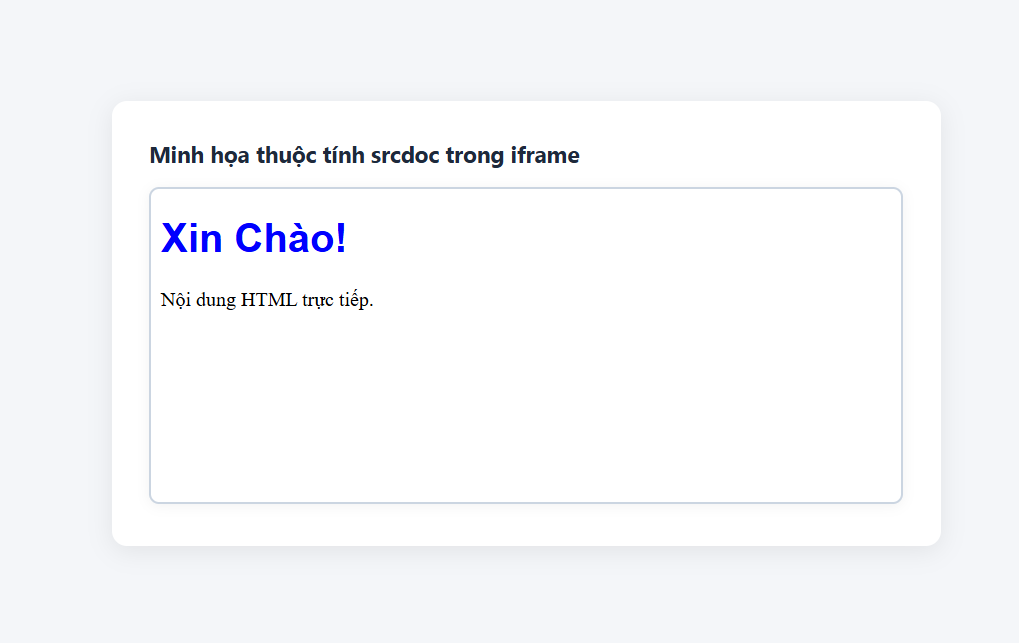
\includegraphics[width=0.7\linewidth]{figures/iframe_srcdoc_result.png}
\end{browserWindow}

% ------------------------------------------------------------------------------
\subsection{Bảng Tra Cứu Toàn Bộ Thuộc Tính Quan Trọng Của <iframe>}

\begin{prettyTableBox}[Bảng Tra Cứu Tất Cả Thuộc Tính Thẻ <iframe> Trong HTML5]
\rowcolors{2}{white}{primaryBlue!4}
\begin{tabularx}{\linewidth}{K{2.4cm} Z Z}
\rowcolor{primaryBlue}
\thd{Thuộc Tính} & \thd{Ý Nghĩa \& Chức Năng Cốt Lõi} & \thd{Ví dụ cú pháp Minh Họa} \\
\codeinline{src} & Đường dẫn URL trỏ tới tài liệu cần nhúng & \codeinline{<iframe src="https://example.com">} \\
\codeinline{srcdoc} & Nhúng trực tiếp chuỗi mã HTML (HTML5) & \codeinline{<iframe srcdoc="<h1>Hi</h1>">} \\
\codeinline{width} & Định nghĩa chiều rộng khung (pixel/percent) & \codeinline{<iframe width="600">} \\
\codeinline{height} & Định nghĩa chiều cao khung (pixel) & \codeinline{<iframe height="400">} \\
\codeinline{frameborder} & 0: Không viền, 1: Có viền (Khuyên dùng CSS) & \codeinline{<iframe frameborder="0">} \\
\codeinline{allowfullscreen} & Bật quyền mở chế độ xem toàn màn hình & \codeinline{<iframe allowfullscreen>} \\
\codeinline{sandbox} & Giới hạn quyền hạn và bảo mật nội dung & \codeinline{<iframe sandbox="allow-scripts">} \\
\codeinline{loading} & \codeinline{lazy} (tải khi cuộn), \codeinline{eager} (tải ngay) & \codeinline{<iframe loading="lazy">} \\
\codeinline{name} & Tên khung để liên kết với thuộc tính \codeinline{target} & \codeinline{<iframe name="myFrame">} \\
\end{tabularx}
\end{prettyTableBox}

% ------------------------------------------------------------------------------
\subsection{4 Trường Hợp Sử Dụng <iframe> Phổ Biến Trong Thực Tế Dự Án}

\paragraph{1. Nhúng một trang web mở (Ví dụ Wikipedia):}
\begin{codeWindow}[Mã Nguồn Nhúng Trang Web Wikipedia Vào Khung Iframe]
\begin{lstlisting}[language=HTML5]
<iframe src="https://www.wikipedia.org/" width="800" height="600"></iframe>
\end{lstlisting}
\end{codeWindow}

\begin{browserWindow}[https://www.wikipedia.org/]
\centering\vspace{2pt}
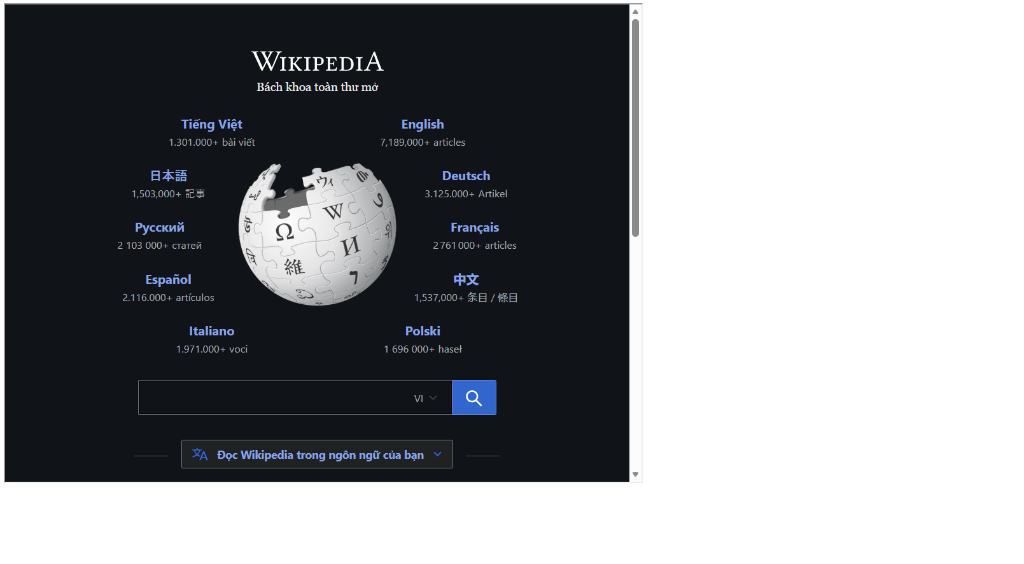
\includegraphics[width=0.7\linewidth]{figures/iframe_wikipedia_result.png}
\end{browserWindow}

\begin{noteBox}[Lưu Ý Quan Trọng Về Chính Sách X-Frame-Options]
Một số trang web lớn (như Google, Facebook) thiết lập Header bảo mật \codeinline{X-Frame-Options: DENY} hoặc \codeinline{SAMEORIGIN} nhằm ngăn chặn trang khác nhúng vào khung iframe để chống tấn công \term{Clickjacking}.
\end{noteBox}

\paragraph{2. Nhúng Video phát trực tuyến từ YouTube:}
YouTube cung cấp đường dẫn nhúng chuẩn qua định dạng \codeinline{/embed/VIDEO\_ID}:
\begin{codeWindow}[Mã Nguồn Nhúng Video YouTube Chuẩn Ngữ Nghĩa]
\begin{lstlisting}[language=HTML5]
<iframe width="560" height="315" 
        src="https://www.youtube.com/embed/dQw4w9WgXcQ" 
        allow="accelerometer; autoplay; clipboard-write; encrypted-media; gyroscope; picture-in-picture"
        allowfullscreen>
</iframe>
\end{lstlisting}
\end{codeWindow}

\begin{browserWindow}[https://www.youtube.com/embed/dQw4w9WgXcQ]
\centering\vspace{2pt}

\includegraphics[width=0.7\linewidth]{figures/iframe_youtube_thumbnail.png}
\end{browserWindow}

\paragraph{3. Nhúng Bản đồ tương tác Google Maps:}
\begin{codeWindow}[Mã Nguồn Nhúng Google Maps Vào Khung Web]
\begin{lstlisting}[language=HTML5]
<iframe width="600" height="450" 
        src="https://www.google.com/maps/embed?pb=!1m18!1m12!1m3!1d3151.835434509839!2d144.9630579153167!3d-37.81410797975171!2m3!1f0!2f0!3f0!3m2!1i1024!2i768!4f13.1!3m3!1m2!1s0x6ad642af0f11fd81%3A0xf5770f9af14bdf8d!2sFederation%20Square!5e0!3m2!1sen!2s!4v1589163966416!5m2!1sen!2s" 
        allowfullscreen>
</iframe>
\end{lstlisting}
\end{codeWindow}

\begin{browserWindow}[https://www.google.com/maps/embed]
\centering\vspace{2pt}
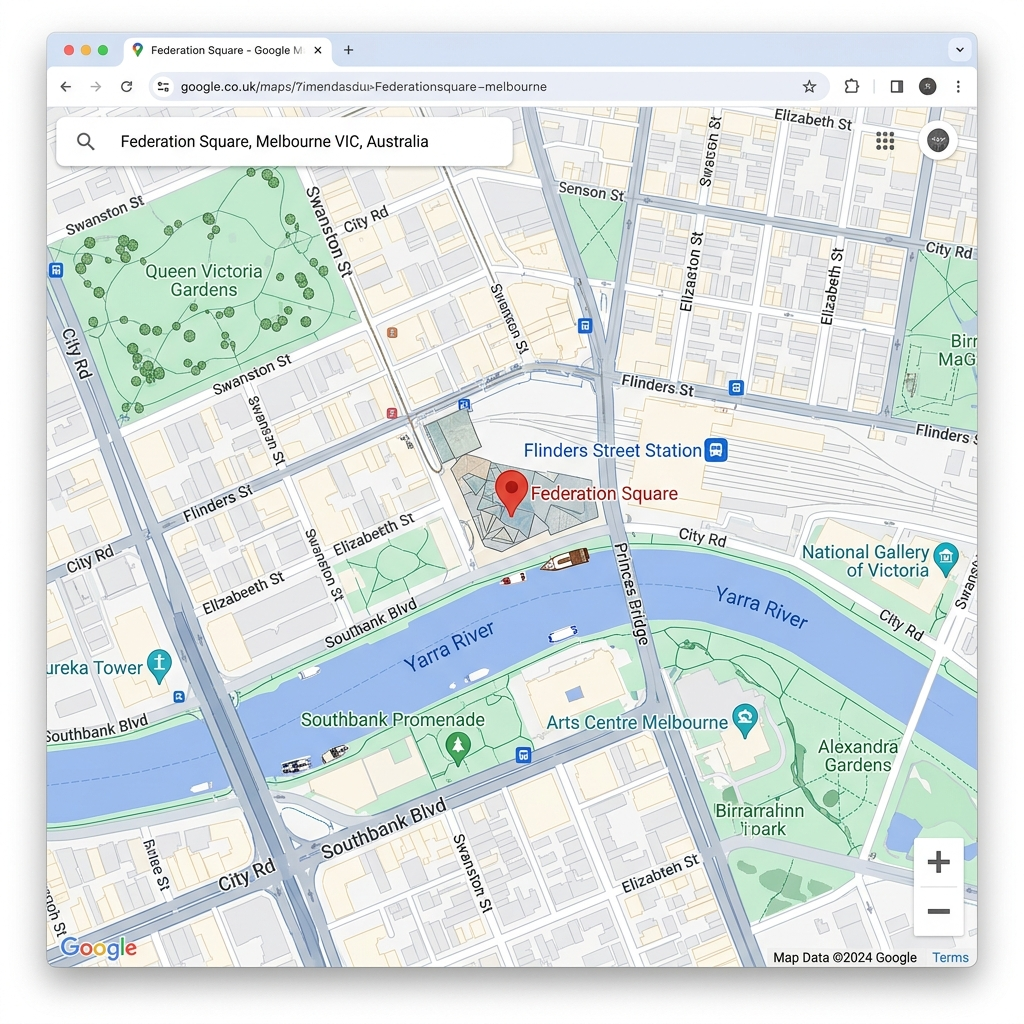
\includegraphics[width=0.7\linewidth]{figures/iframe_google_maps_thumbnail.png}
\end{browserWindow}

\paragraph{4. Nhúng Tài liệu báo cáo dạng tệp PDF:}
\begin{codeWindow}[Mã Nguồn Nhúng Trực Tiếp Tệp Tài Liệu PDF]
\begin{lstlisting}[language=HTML5]
<iframe src="document.pdf" width="800" height="600"></iframe>
\end{lstlisting}
\end{codeWindow}

\begin{browserWindow}[file:///project/document.pdf]
\centering\vspace{2pt}
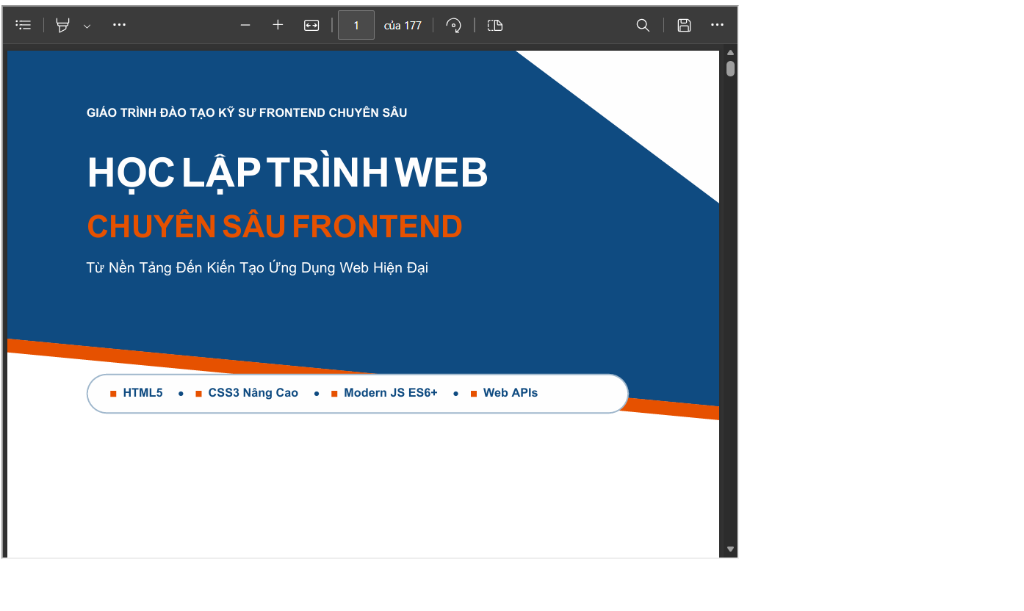
\includegraphics[width=0.7\linewidth]{figures/iframe_pdf_user_real.png}
\end{browserWindow}

% ------------------------------------------------------------------------------
\subsection{Hướng Dẫn Chi Tiết Quy Trình Lấy Đường Dẫn Nhúng (Embed Link)}

Một trong những sai lầm phổ biến nhất của lập trình viên mới bắt đầu là sao chép trực tiếp đường dẫn URL hiển thị trên thanh địa chỉ của trình duyệt để đưa vào thuộc tính \codeinline{src} của thẻ \codeinline{<iframe>}. Các nền tảng lớn như YouTube hay Google Maps đều sử dụng cơ chế bảo mật chống nhúng trực tiếp URL xem thông thường.

\begin{warnBox}[Cảnh Báo Bẫy Sai Lầm Thường Gặp Khi Lấy Link Nhúng]
\begin{itemize}[leftmargin=1.5em, itemsep=3pt, parsep=0pt]
    \item \textbf{SAI}: \codeinline{src="https://www.youtube.com/watch?v=VIDEO\_ID"} $\rightarrow$ Trình duyệt sẽ báo lỗi \term{Refused to display in a frame because it set 'X-Frame-Options' to 'sameorigin'}.
    \item \textbf{ĐÚNG}: \codeinline{src="https://www.youtube.com/embed/VIDEO\_ID"} $\rightarrow$ Sử dụng giao thức nhúng chuẩn do nền tảng cung cấp.
\end{itemize}
\end{warnBox}

\begin{tcolorbox}[enhanced, colback=codeBg, colframe=primaryBlue!30, arc=6pt, boxrule=0.8pt, top=10pt, bottom=10pt, left=12pt, right=12pt, title={\sffamily\bfseries\color{primaryBlue} Quy Trình 4 Bước Lấy Link Nhúng Video YouTube Chuẩn}, coltitle=primaryBlue, colbacktitle=primaryBlue!8, attach boxed title to top left={xshift=10pt, yshift=-10pt}, boxed title style={arc=4pt, boxrule=0.6pt, colframe=primaryBlue!40}]
\vspace{4pt}
\begin{description}[font=\sffamily\bfseries\color{primaryBlue}, leftmargin=4.8em, style=sameline, itemsep=6pt]
    \item[{\tcbox[colback=primaryBlue,coltext=white,boxsep=1pt,left=4pt,right=4pt,top=1pt,bottom=1pt,arc=3pt,fontupper=\sffamily\tiny\bfseries]{BƯỚC 1}}] Mở video cần nhúng trên trang web YouTube.
    \item[{\tcbox[colback=primaryBlue,coltext=white,boxsep=1pt,left=4pt,right=4pt,top=1pt,bottom=1pt,arc=3pt,fontupper=\sffamily\tiny\bfseries]{BƯỚC 2}}] Nhấp vào nút \textbf{Chia sẻ} (\textit{Share}) phía dưới khung phát video.
    \item[{\tcbox[colback=primaryBlue,coltext=white,boxsep=1pt,left=4pt,right=4pt,top=1pt,bottom=1pt,arc=3pt,fontupper=\sffamily\tiny\bfseries]{BƯỚC 3}}] Trong cửa sổ hiện ra, chọn biểu tượng \textbf{Nhúng} (\textit{Embed} - biểu tượng mã \codeinline{</>}).
    \item[{\tcbox[colback=primaryBlue,coltext=white,boxsep=1pt,left=4pt,right=4pt,top=1pt,bottom=1pt,arc=3pt,fontupper=\sffamily\tiny\bfseries]{BƯỚC 4}}] Nhấp nút \textbf{Sao chép} (\textit{Copy}) để lấy toàn bộ đoạn mã \codeinline{<iframe>} đã được tích hợp sẵn thuộc tính chuẩn.
\end{description}
\end{tcolorbox}

\begin{tipBox}[Mẹo Chuyển Đổi Nhanh URL YouTube Thành Embed Link]
Nếu chỉ có URL dạng xem thông thường: \codeinline{https://www.youtube.com/watch?v=dQw4w9WgXcQ}, bạn chỉ cần thay thế cụm \codeinline{watch?v=} bằng \codeinline{embed/} để tạo thành đường dẫn nhúng hợp lệ: \codeinline{https://www.youtube.com/embed/dQw4w9WgXcQ}.
\end{tipBox}

\begin{tcolorbox}[enhanced, colback=codeBg, colframe=secondaryTeal!40, arc=6pt, boxrule=0.8pt, top=10pt, bottom=10pt, left=12pt, right=12pt, title={\sffamily\bfseries\color{secondaryTeal} Quy Trình 4 Bước Lấy Link Nhúng Bản Đồ Google Maps}, coltitle=secondaryTeal, colbacktitle=secondaryTeal!8, attach boxed title to top left={xshift=10pt, yshift=-10pt}, boxed title style={arc=4pt, boxrule=0.6pt, colframe=secondaryTeal!40}]
\vspace{4pt}
\begin{description}[font=\sffamily\bfseries\color{secondaryTeal}, leftmargin=4.8em, style=sameline, itemsep=6pt]
    \item[{\tcbox[colback=secondaryTeal,coltext=white,boxsep=1pt,left=4pt,right=4pt,top=1pt,bottom=1pt,arc=3pt,fontupper=\sffamily\tiny\bfseries]{BƯỚC 1}}] Truy cập Google Maps (\codeinline{maps.google.com}) và tìm kiếm địa điểm/vị trí muốn hiển thị.
    \item[{\tcbox[colback=secondaryTeal,coltext=white,boxsep=1pt,left=4pt,right=4pt,top=1pt,bottom=1pt,arc=3pt,fontupper=\sffamily\tiny\bfseries]{BƯỚC 2}}] Tại bảng thông tin địa điểm ở góc trái, nhấp nút \textbf{Chia sẻ} (\textit{Share}).
    \item[{\tcbox[colback=secondaryTeal,coltext=white,boxsep=1pt,left=4pt,right=4pt,top=1pt,bottom=1pt,arc=3pt,fontupper=\sffamily\tiny\bfseries]{BƯỚC 3}}] Chuyển sang tab \textbf{Nhúng bản đồ} (\textit{Embed a map}).
    \item[{\tcbox[colback=secondaryTeal,coltext=white,boxsep=1pt,left=4pt,right=4pt,top=1pt,bottom=1pt,arc=3pt,fontupper=\sffamily\tiny\bfseries]{BƯỚC 4}}] Chọn kích thước mong muốn (Nhỏ, Vừa, Lớn) rồi nhấp nút \textbf{Sao chép thẻ HTML} (\textit{Copy HTML}).
\end{description}
\end{tcolorbox}

\paragraph{3. Cách nhúng tệp tài liệu PDF cục bộ hoặc trên máy chủ:}
Để nhúng tệp PDF vào trang web, chỉ cần đặt tệp PDF vào cùng thư mục dự án và khai báo đường dẫn tương đối trỏ trực tiếp tới tệp:
\begin{codeWindow}[Khai Báo Nguồn Tệp PDF Trong Cùng Thư Mục Dự Án]
\begin{lstlisting}[language=HTML5]
<!-- (*@Tệp document.pdf nằm cùng cấp thư mục với tệp index.html@*) -->
<iframe src="document.pdf" width="100%" height="600px"></iframe>

<!-- (*@Hoặc trỏ tới thư mục chứa tài liệu tĩnh@*) -->
<iframe src="./assets/pdf/bao-cao-2026.pdf" width="100%" height="600px"></iframe>
\end{lstlisting}
\end{codeWindow}

% ------------------------------------------------------------------------------

% ------------------------------------------------------------------------------
\subsection{Cơ Chế Bảo Mật Tấn Công Clickjacking \& Thuộc Tính sandbox}

\paragraph{Rủi ro bảo mật với Iframe:}
Nếu nhúng một trang web không rõ nguồn gốc, trang đó có thể chạy các kịch bản độc hại, đánh cắp Cookie hoặc đánh lừa người dùng nhấp vào các nút giả mạo (\term{Clickjacking Attack}).

\paragraph{Giải pháp thiết lập thuộc tính sandbox:}
Thuộc tính \codeinline{sandbox} tạo ra một môi trường cách ly (\term{Isolation Sandbox}) cực kỳ nghiêm ngặt. Khi khai báo \codeinline{sandbox}, mặc định trình duyệt sẽ vô hiệu hóa tất cả Script, Form submit, Popup và Same-origin access:
\begin{codeWindow}[Phân Quyền Chi Tiết Cho Iframe Bằng sandbox]
\begin{lstlisting}[language=HTML5]
<iframe src="https://example.com" 
        sandbox="allow-scripts allow-forms">
</iframe>
\end{lstlisting}
\end{codeWindow}

\begin{browserWindow}[https://example.com (sandbox="allow-scripts allow-forms")]
\centering\sffamily\vspace{4pt}
{\bfseries\color{accentOrange}\large Môi Trường Isolation Sandbox Active} \par\vspace{6pt}
\small\textbf{Quyền được cấp:} \codeinline{allow-scripts}, \codeinline{allow-forms} \par\vspace{4pt}
\small\textcolor{warnBorder}{\textbf{Bị khóa hoàn toàn:}} Bị cấm truy cập Cookie, LocalStorage và DOM của trang cha! \par\vspace{4pt}
\end{browserWindow}

% ------------------------------------------------------------------------------
\subsection{Kỹ Thuật Loại Bỏ Viền \& Định Kiểu CSS Hiện Đại}

Mặc định thẻ \codeinline{<iframe>} có đường viền 3D cổ điển. Trong thực tế dự án, lập trình viên sử dụng CSS để loại bỏ viền và làm mịn giao diện:

\begin{codeWindow}[Loại Bỏ Viền Iframe Bằng CSS3]
\begin{lstlisting}[language=HTML5]
<style>
  iframe {
      border: none;
      border-radius: 8px;
      box-shadow: 0 4px 12px rgba(0,0,0,0.1);
  }
</style>
\end{lstlisting}
\end{codeWindow}

\begin{browserWindow}[https://example.com (style="border: none; border-radius: 8px;")]
\centering\sffamily\vspace{4pt}
{\bfseries\color{tipBorder}\large Giao Diện Khung Iframe Đã Loại Bỏ Viền Bằng CSS} \par\vspace{6pt}
\small\color{darkText} Đường viền 3D thô cứng bị xóa hoàn toàn, thay bằng góc bo 8px và bóng mờ nhẹ sang trọng. \par\vspace{4pt}
\end{browserWindow}

% ------------------------------------------------------------------------------
\subsection{Bảng Đánh Giá Ưu Điểm \& Nhược Điểm Của <iframe>}

\begin{prettyTableBox}[Bảng Tổng Hợp Đánh Giá Ưu Điểm Và Nhược Điểm Của <iframe>]
\rowcolors{2}{white}{primaryBlue!4}
\begin{tabularx}{\linewidth}{Z Z}
\rowcolor{primaryBlue}
\thd{Ưu Điểm Nổi Bật} & \thd{Nhược Điểm \& Hạn Chế} \\
Nhúng dễ dàng nội dung độc lập từ website bên ngoài & Một số trang web chặn nhúng bằng Header \codeinline{X-Frame-Options} \\
Hỗ trợ trình chiếu Video YouTube, Bản đồ Maps, Tài liệu PDF & Làm tăng số lượng HTTP Requests, ảnh hưởng hiệu năng tải trang \\
Kiểm soát phân quyền bảo mật độc lập bằng \codeinline{sandbox} & Tiềm ẩn rủi ro tấn công Clickjacking nếu không kiểm soát \\
\end{tabularx}
\end{prettyTableBox}

% ------------------------------------------------------------------------------
\subsection{Chuyên Sâu Thuộc Tính name \& Kỹ Thuật Điều Hướng target}

\paragraph{1. Định nghĩa thuộc tính name trong <iframe>:}
Thuộc tính \codeinline{name} được sử dụng để đặt danh xưng cho khung iframe. Mục đích chính là làm điểm nhận kết quả (\term{Target Destination}) cho các thẻ liên kết \codeinline{<a target="...">} hoặc thẻ biểu mẫu \codeinline{<form target="...">}, giúp nạp nội dung mới vào trong iframe mà \textbf{KHÔNG CẦN TẢI LẠI TRANG CHÍNH}.

\paragraph{2. Ví dụ 1: Điều hướng nội dung tìm kiếm Cốc Cốc vào iframe Bing:}
\begin{codeWindow}[Mã Nguồn Liên Kết Thẻ <a> Với name Của <iframe>]
\begin{lstlisting}[language=HTML5]
<!-- (*@Khung Iframe hiển thị Bing mặc định, có tên@*) name="web_bing" -->
<iframe src="https://www.bing.com/" name="web_bing" width="1000" height="600"></iframe>

<!-- (*@Thẻ a trỏ target tới@*) name="web_bing" (*@của iframe@*) -->
<p>
  <a href="https://coccoc.com/search" target="web_bing">
    (*@Tìm kiếm trên Cốc Cốc@*)
  </a>
</p>
\end{lstlisting}
\end{codeWindow}

\begin{browserWindow}[https://www.bing.com (name="web\_bing")]
\centering\sffamily\vspace{4pt}
{\bfseries\color{primaryBlue}\large Khung Iframe nhận tín hiệu điều hướng: name="web\_bing"} \par\vspace{6pt}
\small Ban đầu hiển thị: \textcolor{primaryBlue}{\underline{https://www.bing.com/}} \par\vspace{4pt}
\small\textcolor{accentOrange}{$\rightarrow$ Khi nhấp liên kết bên dưới, nội dung tải Cốc Cốc trực tiếp vào khung này!} \par\vspace{8pt}
\textcolor{primaryBlue}{\underline{Tìm kiếm trên Cốc Cốc}} \quad \small\textcolor{codeComment}{(target="web\_bing")} \par\vspace{4pt}
\end{browserWindow}

\paragraph{Phân tích trình tự hoạt động chi tiết:}
\begin{description}[font=\sffamily\bfseries\color{primaryBlue}, leftmargin=4.8em, style=sameline, itemsep=4pt]
    \item[{\tcbox[colback=primaryBlue,coltext=white,boxsep=1pt,left=4pt,right=4pt,top=1pt,bottom=1pt,arc=3pt,fontupper=\sffamily\tiny\bfseries]{BƯỚC 1}}] Khi tải trang ban đầu, iframe nạp trang Bing (\codeinline{src="https://www.bing.com/"}).
    \item[{\tcbox[colback=primaryBlue,coltext=white,boxsep=1pt,left=4pt,right=4pt,top=1pt,bottom=1pt,arc=3pt,fontupper=\sffamily\tiny\bfseries]{BƯỚC 2}}] Người dùng nhấp vào đường link \textit{"Tìm kiếm trên Cốc Cốc"}.
    \item[{\tcbox[colback=primaryBlue,coltext=white,boxsep=1pt,left=4pt,right=4pt,top=1pt,bottom=1pt,arc=3pt,fontupper=\sffamily\tiny\bfseries]{BƯỚC 3}}] Do thẻ \codeinline{<a>} có thuộc tính \codeinline{target="web\_bing"}, trình duyệt tải trực tiếp nội dung Cốc Cốc vào khung iframe \codeinline{name="web\_bing"}.
\end{description}

\paragraph{Phân biệt thuộc tính target trong thẻ <a>:}
\begin{itemize}[leftmargin=1.8em, itemsep=3pt, parsep=0pt]
    \item \codeinline{target="\_blank"}: Mở liên kết trong một Tab / Cửa sổ mới.
    \item \codeinline{target="\_self"}: Mở liên kết ngay tại Tab hiện tại (Mặc định).
    \item \codeinline{target="tên\_iframe"}: Mở liên kết bên trong khung iframe có \codeinline{name="tên\_iframe"}.
\end{itemize}

\paragraph{3. Ví dụ 2: Điều hướng bài viết Wikipedia trong Iframe:}
\begin{codeWindow}[Mã Nguồn Liên Kết Bài Viết Wikipedia Vào Frame wiki\_frame]
\begin{lstlisting}[language=HTML5]
<iframe src="https://www.wikipedia.org/" name="wiki_frame" width="1000" height="600"></iframe>

<p>
  <a href="https://vi.wikipedia.org/wiki/Lap_trinh" target="wiki_frame">
    (*@Xem bài viết về Lập trình trên Wikipedia@*)
  </a>
</p>
\end{lstlisting}
\end{codeWindow}

\begin{browserWindow}[https://vi.wikipedia.org/wiki/Lap\_trinh (name="wiki\_frame")]
\centering\sffamily\vspace{4pt}
{\bfseries\color{primaryBlue}\large Nạp Bài Viết Lập Trình Vào Khung wiki\_frame} \par\vspace{6pt}
{\small\color{darkText} Nạp bài viết Lập trình trực tiếp vào khung mà không làm chuyển trang chính.} \par\vspace{4pt}
\textcolor{primaryBlue}{\underline{Xem bài viết về Lập trình trên Wikipedia}} \quad \small\textcolor{codeComment}{(target="wiki\_frame")} \par\vspace{4pt}
\end{browserWindow}

\paragraph{4. Ví dụ 3: Gửi dữ liệu Form kết quả vào khung Iframe:}
\begin{codeWindow}[Mã Nguồn Gửi Kết Quả Submit Form Trực Tiếp Vào Iframe]
\begin{lstlisting}[language=HTML5]
<iframe name="formResult" width="600" height="300"></iframe>

<form action="https://www.example.com/search" target="formResult">
    <input type="text" name="query" placeholder="(*@Nhập từ khóa...@*)">
    <button type="submit">(*@Tìm kiếm@*)</button>
</form>
\end{lstlisting}
\end{codeWindow}

\begin{browserWindow}[https://www.example.com/search?query=HTML5 (name="formResult")]
\centering\sffamily\vspace{4pt}
{\bfseries\color{secondaryTeal}\large Kết Quả Submit Form Hiển Thị Trong Khung formResult} \par\vspace{6pt}
{\small\color{darkText} Khi bấm Tìm kiếm, trang kết quả hiển thị trực tiếp ngay trong khung mà không làm nạp lại trang hiện tại.} \par\vspace{4pt}
\end{browserWindow}

% ------------------------------------------------------------------------------
\subsection{Phân Biệt Chi Tiết Thuộc Tính name Và id Trong <iframe>}

\begin{prettyTableBox}[Bảng So Sánh Chi Tiết Giữa Thuộc Tính name Và id Của <iframe>]
\rowcolors{2}{white}{primaryBlue!4}
\begin{tabularx}{\linewidth}{K{2.5cm} Z Z}
\rowcolor{primaryBlue}
\thd{Tiêu Chí So Sánh} & \thd{Thuộc Tính name} & \thd{Thuộc Tính id} \\
Mục đích chính & Định danh iframe để làm đích đến cho thuộc tính \codeinline{target} & Định danh duy nhất để thao tác với CSS hoặc JavaScript \\
Tính trùng lặp & Có thể lặp lại tên trên nhiều phần tử & \textbf{Tuyệt đối duy nhất} trên toàn trang \\
Tương tác \codeinline{target} & \textbf{Sử dụng trực tiếp} với \codeinline{<a target="...">} & Không thể dùng làm giá trị cho \codeinline{target} \\
Thao tác JavaScript & Ít phổ biến & \textbf{Rất phổ biến} (\codeinline{document.getElementById}) \\
\end{tabularx}
\end{prettyTableBox}

\begin{conceptBox}[Ma Trận Khi Nào Dùng name Và Khi Nào Dùng id Của Iframe]
\begin{itemize}[leftmargin=1.5em, itemsep=3pt, parsep=0pt]
    \item \textbf{Dùng name}: Khi muốn điều hướng liên kết \codeinline{<a target="name">} hoặc kết quả Form \codeinline{<form target="name">} vào bên trong iframe.
    \item \textbf{Dùng id}: Khi muốn áp dụng CSS (\codeinline{\#myFrame \{ border: none; \}}) hoặc lập trình JavaScript (\codeinline{document.getElementById("myFrame")}).
\end{itemize}
\end{conceptBox}

% ==============================================================================
% CHUYÊN ĐỀ CHUYÊN SÂU: THẺ SEMANTIC TRONG HTML5 (SEMANTIC HTML5 MASTERCLASS)
% ==============================================================================
\section{Chi Tiết Về Các Thẻ Semantic Trong HTML}
\label{sec:semantic_html5_masterclass}

\subsection{Thẻ Semantic Là Gì?}

\term{Thẻ Semantic (thẻ có ý nghĩa)} là các thẻ HTML mô tả ý nghĩa của nội dung bên trong nó thay vì chỉ đơn thuần là một khối (\codeinline{<div>}) hoặc một dòng (\codeinline{<span>}).

\begin{itemize}[leftmargin=1.8em, itemsep=4pt, parsep=0pt]
    \item \textbf{Bản chất kỹ thuật}: Cung cấp thông tin ngữ nghĩa rõ ràng cho cả máy tính (trình duyệt, công cụ tìm kiếm, trình đọc màn hình) và con người (lập trình viên).
    \item \textbf{Mục đích cốt lõi}: Giúp trình duyệt, công cụ tìm kiếm (SEO) và lập trình viên hiểu nội dung dễ dàng hơn.
\end{itemize}

\subsubsection{Ví Dụ So Sánh Trực Quan Giữa Thẻ Div Và Thẻ Semantic}

\begin{prettyTableBox}[So Sánh Cú Pháp: Non-Semantic (Div) vs. Semantic HTML5]
\rowcolors{2}{white}{primaryBlue!4}
\begin{tabularx}{\linewidth}{>{\sffamily\bfseries\color{primaryBlue}}C{3.0cm} Z Z}
\rowcolor{primaryBlue}
\thd{\sffamily Vùng Thành Phần} & \thd{\sffamily [Khó Bảo Trì] Cấu Trúc Div Soup} & \thd{\sffamily [Dễ Bảo Trì] Chuẩn Semantic HTML5} \\
Phần đầu trang & \codeinline{<div class="header">...</div>} & \codeinline{<header>...</header>} \\
Thanh điều hướng & \codeinline{<div class="nav">...</div>} & \codeinline{<nav>...</nav>} \\
Nội dung chính & \codeinline{<div class="content">...</div>} & \codeinline{<main>...</main>} \\
Chân trang & \codeinline{<div class="footer">...</div>} & \codeinline{<footer>...</footer>} \\
\end{tabularx}
\end{prettyTableBox}


\subsubsection{Sơ Đồ Minh Họa Bố Cục Trang Web: Div Soup vs Semantic Landmarks}

\begin{center}
\begin{tcolorbox}[
    enhanced,
    colback=codeBg!40!white,
    colframe=primaryBlue!30,
    arc=8pt,
    boxrule=0.8pt,
    drop shadow=black!4!white,
    top=14pt, bottom=14pt, left=10pt, right=10pt,
    title={\sffamily\bfseries\small\color{primaryBlue} SƠ ĐỒ SO SÁNH KIẾN TRÚC TRANG WEB: KHÔNG SEMANTIC VS SEMANTIC HTML5}
]
\centering
\begin{tikzpicture}[
    scale=0.85, transform shape,
    font=\sffamily\small,
    divNode/.style={fill=red!8, draw=red!50, rounded corners=3pt, inner sep=3pt, font=\fontsize{7pt}{9pt}\selectfont\ttfamily\bfseries\color{red!80!black}, align=center},
    semNode/.style={fill=primaryBlue!10, draw=primaryBlue!70, rounded corners=3pt, inner sep=3pt, font=\fontsize{7pt}{9pt}\selectfont\ttfamily\bfseries\color{primaryBlue}, align=center},
    arrowLine/.style={->, >=stealth, line width=1.5pt, color=accentOrange}
]

% Left Column: Non-semantic Div structure (x = 0 to 5.2cm, center at x = 2.6)
\node[divNode, minimum width=5.2cm] (dhead) at (2.6, 0) {<div class="header"> Header </div>};
\node[divNode, minimum width=5.2cm] (dnav) at (2.6, -0.75) {<div class="nav"> Navigation </div>};
\node[divNode, minimum width=3.3cm, minimum height=1.6cm] (dmain) at (1.65, -2.1) {<div class="content">\\Main Content\\</div>};
\node[divNode, minimum width=1.7cm, minimum height=1.6cm] (dside) at (4.35, -2.1) {<div class="side">\\Sidebar\\</div>};
\node[divNode, minimum width=5.2cm] (dfoot) at (2.6, -3.45) {<div class="footer"> Footer </div>};
\node[font=\sffamily\bfseries\small\color{red!80!black}] at (2.6, 0.65) {[Khó Bảo Trì] "Div Soup"};

% Middle Connecting Arrow (x = 5.2 to 7.8, arrow from 5.5 to 7.5)
\draw[arrowLine] (5.5, -2.1) -- (7.5, -2.1) 
    node[midway, above=3pt, font=\sffamily\bfseries\tiny\color{accentOrange}] {NÂNG CẤP}
    node[midway, below=3pt, font=\sffamily\tiny\color{darkText!70}] {Thẻ Ngữ Nghĩa};

% Right Column: Semantic HTML5 structure (x = 7.8 to 13.0cm, center at x = 10.4)
\node[semNode, minimum width=5.2cm] (shead) at (10.4, 0) {<header> Header </header>};
\node[semNode, minimum width=5.2cm] (snav) at (10.4, -0.75) {<nav> Navigation </nav>};
\node[semNode, minimum width=3.3cm, minimum height=1.6cm] (smain) at (9.45, -2.1) {<main>\\<article> Content </article>\\</main>};
\node[semNode, minimum width=1.7cm, minimum height=1.6cm] (sside) at (12.15, -2.1) {<aside>\\Sidebar\\</aside>};
\node[semNode, minimum width=5.2cm] (sfoot) at (10.4, -3.45) {<footer> Footer </footer>};
\node[font=\sffamily\bfseries\small\color{primaryBlue}] at (10.4, 0.65) {[Dễ Bảo Trì] Semantic HTML5};

\end{tikzpicture}
\end{tcolorbox}
\end{center}

% ==============================================================================
\subsection{Lợi Ích Của Thẻ Semantic}

Sử dụng thẻ Semantic mang lại 4 lợi ích lớn trong phát triển web chuyên nghiệp:

\begin{itemize}[leftmargin=1.8em, itemsep=6pt, parsep=0pt]
    \item \textbf{Tối ưu SEO}: Công cụ tìm kiếm dễ hiểu nội dung, giúp trang xếp hạng cao hơn trên kết quả tìm kiếm (Google, Bing).
    \item \textbf{Hỗ trợ truy cập (Accessibility - A11y)}: Người khiếm thị có thể sử dụng trình đọc màn hình (\textit{Screen Readers}) để điều hướng trang web dễ dàng hơn.
    \item \textbf{Dễ bảo trì \& nâng cấp}: Mã nguồn rõ ràng, dễ đọc, dễ hiểu cho lập trình viên khác khi tham gia vào dự án.
    \item \textbf{Giúp CSS dễ quản lý hơn}: Dùng đúng thẻ giúp giảm bớt class và ID không cần thiết trong tập tin CSS.
\end{itemize}

% ==============================================================================
\subsection{Danh Sách Các Thẻ Semantic Và Cách Sử Dụng}

Dưới đây là tổng hợp đầy đủ danh sách các thẻ Semantic phổ biến trong HTML5, chức năng kỹ thuật và ví dụ cú pháp đại diện:

\begin{prettyTableBox}[Danh Sách Các Thẻ Semantic HTML5 Và Ví Dụ Minh Họa]
\rowcolors{2}{white}{primaryBlue!4}
\begin{tabularx}{\linewidth}{>{\ttfamily\bfseries\color{primaryBlue}}K{2.2cm} Z Z}
\rowcolor{primaryBlue}
\thd{\sffamily Thẻ Semantic} & \thd{\sffamily Chức năng} & \thd{\sffamily Ví dụ minh họa cú pháp} \\

<header> & Phần đầu trang web (chứa logo, menu, tiêu đề). & \codeinline{<header><h1>Header</h1>}\newline\codeinline{</header>} \\

<nav> & Thanh điều hướng chứa menu liên kết. & \codeinline{<nav><a href="\#">Home</a></nav>} \\

<main> & Nội dung chính của trang web. & \codeinline{<main><h2>Nội dung</h2></main>} \\

<section> & Chia nội dung thành từng phần có chủ đề riêng. & \codeinline{<section><h2>Giới thiệu</h2></section>} \\

<article> & Bài viết độc lập như blog, tin tức. & \codeinline{<article><h2>Bài viết mới</h2></article>} \\

<aside> & Nội dung phụ như sidebar, quảng cáo. & \codeinline{<aside><h3>Tin liên quan</h3></aside>} \\

<footer> & Chân trang, chứa bản quyền, liên hệ. & \codeinline{<footer><p>\&copy; 2026</p></footer>} \\

<address> & Hiển thị thông tin liên hệ tác giả. & \codeinline{<address>info@example.com}\newline\codeinline{</address>} \\

<figure> & Nhóm hình ảnh hoặc biểu đồ minh họa. & \codeinline{<figure><img src="img.jpg"></figure>} \\

<figcaption> & Chú thích cho hình ảnh (dùng trong \codeinline{<figure>}). & \codeinline{<figcaption>Chú thích ảnh</figcaption>} \\

<mark> & Đánh dấu văn bản quan trọng (tô vàng). & \codeinline{<mark>Nội dung quan trọng</mark>} \\

<time> & Hiển thị ngày/giờ chuẩn máy đọc. & \codeinline{<time datetime="2026-07-26">}\newline\codeinline{  26/07/2026</time>} \\

<summary> & Tiêu đề cho nội dung thu gọn \codeinline{<details>}. & \codeinline{<summary>Xem chi tiết</summary>} \\

<details> & Hiển thị nội dung thu gọn/mở rộng khi click. & \codeinline{<details>}\newline\codeinline{  <summary>Mở</summary>}\newline\codeinline{</details>} \\

<dialog> & Hộp thoại pop-up trong HTML5. & \codeinline{<dialog open>Thông báo</dialog>} \\

<cite> & Trích dẫn nguồn tài liệu, bài báo. & \codeinline{<cite>HTML Mastery</cite>} \\

<code> & Hiển thị đoạn mã lập trình. & \codeinline{<code>console.log('Hi');</code>} \\
\end{tabularx}
\end{prettyTableBox}

% ==============================================================================
\subsection{Ví Dụ Sử Dụng Thực Tế Trong Một Trang Web}

Mã nguồn dưới đây minh họa cách kết hợp các thẻ Semantic để tạo dựng một cấu trúc trang web hoàn chỉnh tiêu chuẩn HTML5:

\begin{codeWindow}[Mã Nguồn Trang Web HTML5 Hoàn Chỉnh Sử Dụng Thẻ Semantic]
\begin{lstlisting}[language=HTML5]
<!DOCTYPE html>
<html lang="vi">
<head>
    <meta charset="UTF-8">
    <meta name="viewport" content="width=device-width, initial-scale=1.0">
    <title>(*@Website với Semantic HTML@*)</title>
</head>
<body>
    <header>
        <h1>(*@Website của tôi@*)</h1>
    </header>
    <nav>
        <a href="#">(*@Trang chủ@*)</a> | <a href="#">(*@Giới thiệu@*)</a> | <a href="#">(*@Liên hệ@*)</a>
    </nav>
    <main>
        <article>
            <h2>(*@Bài viết đầu tiên@*)</h2>
            <p>(*@Đây là nội dung bài viết.@*)</p>
        </article>
    </main>
    <aside>
        <h3>(*@Bài viết liên quan@*)</h3>
        <p>(*@Thêm nội dung hữu ích.@*)</p>
    </aside>
    <footer>
        <p>&copy; 2025 - (*@Bản quyền thuộc về tôi.@*)</p>
    </footer>
</body>
</html>
\end{lstlisting}
\end{codeWindow}

% ==============================================================================
\subsection{Tổng Kết: Vì Sao Nên Dùng Thẻ Semantic?}

\begin{prettyTableBox}[Tóm Tắt Lý Do Bắt Buộc Dùng Thẻ Semantic Trong Phát Triển Web]
\rowcolors{2}{white}{primaryBlue!4}
\begin{tabularx}{\linewidth}{>{\bfseries\color{primaryBlue}}C{4.5cm} Z}
\rowcolor{primaryBlue}
\thd{\sffamily Lợi ích} & \thd{\sffamily Lý do} \\
SEO tốt hơn & Công cụ tìm kiếm hiểu nội dung dễ dàng hơn. \\
Hỗ trợ người khuyết tật & Trình đọc màn hình đọc trang tốt hơn. \\
Dễ bảo trì code & Lập trình viên khác dễ hiểu cấu trúc trang web. \\
Dễ chỉnh sửa CSS & Nhắm đúng thẻ không cần nhiều class. \\
\end{tabularx}
\end{prettyTableBox}

\begin{conceptBox}[Tóm Lại]
Nên dùng thẻ Semantic thay vì \codeinline{<div>} nếu có thể, vì nó giúp trang web rõ ràng, dễ hiểu, thân thiện với SEO \& dễ bảo trì hơn!
\end{conceptBox}

% ==============================================================================
\subsection{Phân Tích Chi Tiết Danh Sách Một Số Thẻ Semantic Phổ Biến}

\subsubsection{1. Thẻ \codeinline{<header>} -- Phần Đầu Trang}
\textbf{Chức năng}: Chứa tiêu đề, logo, menu điều hướng, hoặc thông tin đầu trang.

\begin{codeWindow}[Mã Nguồn Mẫu Khai Báo Thẻ <header>]
\begin{lstlisting}[language=HTML5]
<header>
    <h1>(*@Chào mừng đến với Website@*)</h1>
    <nav>
        <ul>
            <li><a href="#">(*@Trang chủ@*)</a></li>
            <li><a href="#">(*@Giới thiệu@*)</a></li>
            <li><a href="#">(*@Liên hệ@*)</a></li>
        </ul>
    </nav>
</header>
\end{lstlisting}
\end{codeWindow}

\subsubsection{2. Thẻ \codeinline{<nav>} -- Thanh Điều Hướng}
\textbf{Chức năng}: Chứa danh sách liên kết để điều hướng trang web.

\begin{codeWindow}[Mã Nguồn Mẫu Khai Báo Thẻ <nav>]
\begin{lstlisting}[language=HTML5]
<nav>
    <ul>
        <li><a href="#">(*@Trang chủ@*)</a></li>
        <li><a href="#">(*@Sản phẩm@*)</a></li>
        <li><a href="#">(*@Liên hệ@*)</a></li>
    </ul>
</nav>
\end{lstlisting}
\end{codeWindow}

\begin{noteBox}[Lưu ý khi sử dụng thẻ <nav>]
Nên dùng \codeinline{<nav>} khi có nhóm liên kết chính, nếu chỉ có vài link nhỏ trong bài viết thì không cần.
\end{noteBox}

\subsubsection{3. Thẻ \codeinline{<section>} -- Phần Nội Dung}
\textbf{Chức năng}: Dùng để chia nội dung thành từng phần riêng biệt.

\begin{codeWindow}[Mã Nguồn Mẫu Khai Báo Thẻ <section>]
\begin{lstlisting}[language=HTML5]
<section>
    <h2>(*@Sản phẩm nổi bật@*)</h2>
    <p>(*@Danh sách các sản phẩm bán chạy nhất...@*)</p>
</section>
\end{lstlisting}
\end{codeWindow}

\begin{noteBox}[Lưu ý khi sử dụng thẻ <section>]
Dùng \codeinline{<section>} khi nội dung có chủ đề riêng và có tiêu đề (\codeinline{<h2>}, \codeinline{<h3>}...). Nếu không có tiêu đề, có thể dùng \codeinline{<div>} thay thế.
\end{noteBox}

\subsubsection{4. Thẻ \codeinline{<article>} -- Bài Viết Độc Lập}
\textbf{Chức năng}: Dùng cho nội dung tự tồn tại (bài báo, blog, tin tức).

\begin{codeWindow}[Mã Nguồn Mẫu Khai Báo Thẻ <article>]
\begin{lstlisting}[language=HTML5]
<article>
    <h2>(*@Học HTML5 cơ bản@*)</h2>
    <p>(*@HTML5 mang lại nhiều tính năng mới giúp lập trình viên...@*)</p>
</article>
\end{lstlisting}
\end{codeWindow}

\begin{conceptBox}[Phân biệt giữa <article> và <section>]
\begin{itemize}[leftmargin=1.5em, itemsep=2pt, parsep=0pt]
    \item \codeinline{<article>}: Nội dung có thể đọc độc lập (blog, tin tức).
    \item \codeinline{<section>}: Chỉ là phần trong trang web, thường có nhiều bài viết nhỏ.
\end{itemize}
\end{conceptBox}

\subsubsection{5. Thẻ \codeinline{<aside>} -- Nội Dung Bên Lề}
\textbf{Chức năng}: Dùng cho quảng cáo, danh sách liên quan, thanh bên (sidebar).

\begin{codeWindow}[Mã Nguồn Mẫu Khai Báo Thẻ <aside>]
\begin{lstlisting}[language=HTML5]
<aside>
    <h3>(*@Bài viết liên quan@*)</h3>
    <ul>
        <li><a href="#">(*@HTML cơ bản@*)</a></li>
        <li><a href="#">(*@CSS nâng cao@*)</a></li>
    </ul>
</aside>
\end{lstlisting}
\end{codeWindow}

\begin{noteBox}[Lưu ý khi sử dụng thẻ <aside>]
Nội dung không liên quan trực tiếp đến phần chính nhưng vẫn có ích.
\end{noteBox}

\subsubsection{6. Thẻ \codeinline{<footer>} -- Chân Trang}
\textbf{Chức năng}: Chứa thông tin bản quyền, liên hệ, link quan trọng.

\begin{codeWindow}[Mã Nguồn Mẫu Khai Báo Thẻ <footer>]
\begin{lstlisting}[language=HTML5]
<footer>
    <p>&copy; 2026 (*@Bản quyền thuộc về Website của tôi@*)</p>
    <p><a href="mailto:contact@example.com">(*@Liên hệ@*)</a></p>
</footer>
\end{lstlisting}
\end{codeWindow}

\begin{noteBox}[Lưu ý khi sử dụng thẻ <footer>]
Có thể có nhiều \codeinline{<footer>} trên trang, ví dụ trong mỗi \codeinline{<article>}.
\end{noteBox}

\subsubsection{7. Thẻ \codeinline{<figure>} Và \codeinline{<figcaption>} -- Ảnh Minh Họa}
\textbf{Chức năng}: Dùng để nhóm hình ảnh hoặc đồ họa với chú thích.


\begin{codeWindow}[Mã Nguồn Mẫu Khai Báo Thẻ <figure> và <figcaption>]
\begin{lstlisting}[language=HTML5]
<figure>
    <img src="image.jpg" alt="(*@Hình ảnh mô tả@*)">
    <figcaption>(*@Hình ảnh minh họa cho bài viết@*)</figcaption>
</figure>
\end{lstlisting}
\end{codeWindow}

\begin{noteBox}[Lưu ý khi sử dụng thẻ <figcaption>]
\codeinline{<figcaption>} là tùy chọn, giúp mô tả ảnh mà không cần thêm \codeinline{<p>}.
\end{noteBox}

% ==============================================================================
\subsection{Phân Tích Chuyên Sâu 4 Lý Do Vì Sao Nên Dùng Thẻ Semantic}

Thẻ Semantic giúp trang web có cấu trúc rõ ràng hơn so với việc chỉ sử dụng \codeinline{<div>}. Dưới đây là phân tích chi tiết 4 lý do chính:

\subsubsection{1. Giúp Trình Duyệt \& Công Cụ Tìm Kiếm (SEO) Hiểu Nội Dung Trang Web}
\begin{itemize}[leftmargin=1.8em, itemsep=3pt, parsep=0pt]
    \item Google, Bing, Cốc Cốc và các công cụ tìm kiếm khác có thể đọc hiểu trang web dễ dàng hơn nếu sử dụng các thẻ Semantic.
    \item Giúp xếp hạng SEO tốt hơn vì công cụ tìm kiếm có thể phân loại nội dung chính, nội dung phụ.
\end{itemize}

\begin{prettyTableBox}[So Sánh Giữa Khai Báo Không Rõ Ràng (Div) Và Khai Báo Semantic Rõ Ràng]
\rowcolors{2}{white}{primaryBlue!4}
\begin{tabularx}{\linewidth}{>{\sffamily\bfseries\color{primaryBlue}}C{3.0cm} Z Z}
\rowcolor{primaryBlue}
\thd{\sffamily Vùng Giao Diện} & \thd{\sffamily [Không Rõ Ràng] Dùng <div>} & \thd{\sffamily [Rõ Ràng] Dùng Thẻ Semantic} \\
Phần đầu trang & \codeinline{<div class="top">...</div>} & \codeinline{<header>...</header>} \\
Thanh menu & \codeinline{<div class="nav">...</div>} & \codeinline{<nav>...</nav>} \\
Nội dung chính & \codeinline{<div class="content">...</div>} & \codeinline{<main>...</main>} \\
Chân trang & \codeinline{<div class="bottom">...</div>} & \codeinline{<footer>...</footer>} \\
\end{tabularx}
\end{prettyTableBox}

\subsubsection{2. Cải Thiện Khả Năng Truy Cập (Accessibility - A11y) Cho Người Dùng Khuyết Tật}
\begin{itemize}[leftmargin=1.8em, itemsep=3pt, parsep=0pt]
    \item Trình đọc màn hình (\textit{screen readers}) có thể đọc hiểu nội dung dễ dàng hơn nếu dùng thẻ Semantic.
    \item Hỗ trợ người khiếm thị điều hướng trang web tốt hơn.
\end{itemize}

\begin{noteBox}[Minh Họa Tác Động Truy Cập (A11y)]
\begin{itemize}[leftmargin=1.5em, itemsep=2pt, parsep=0pt]
    \item Nếu có \codeinline{<nav>}, trình đọc màn hình biết đây là thanh menu thay vì chỉ là một \codeinline{<div>}.
    \item Nếu có \codeinline{<article>}, họ biết đây là nội dung chính thay vì phải đoán.
\end{itemize}
\end{noteBox}

\subsubsection{3. Dễ Bảo Trì \& Mở Rộng Code (Dễ Đọc Hiểu Hơn)}
\begin{itemize}[leftmargin=1.8em, itemsep=3pt, parsep=0pt]
    \item Nếu dùng thẻ Semantic, lập trình viên mới vào dự án dễ hiểu code hơn.
    \item Khi sửa hoặc cập nhật nội dung, dễ dàng tìm đúng vị trí cần chỉnh sửa.
\end{itemize}

\begin{prettyTableBox}[So Sánh Cấu Trúc Khó Bảo Trì Và Dễ Bảo Trì Trong Dự Án Web]
\rowcolors{2}{white}{primaryBlue!4}
\begin{tabularx}{\linewidth}{>{\sffamily\bfseries\color{primaryBlue}}C{3.0cm} Z Z}
\rowcolor{primaryBlue}
\thd{\sffamily Phần Tử Web} & \thd{\sffamily [Khó Bảo Trì] Dùng Div ID} & \thd{\sffamily [Dễ Bảo Trì] Dùng Thẻ Semantic} \\
Khối tiêu đề & \codeinline{<div id="header">...</div>} & \codeinline{<header>...</header>} \\
Khối menu & \codeinline{<div id="menu">...</div>} & \codeinline{<nav>...</nav>} \\
Khối nội dung & \codeinline{<div id="content">...</div>} & \codeinline{<main>...</main>} \\
Khối chân trang & \codeinline{<div id="footer">...</div>} & \codeinline{<footer>...</footer>} \\
\end{tabularx}
\end{prettyTableBox}
\begin{center}
$\rightarrow$ \textbf{Kết luận}: Dễ nhìn, dễ hiểu, dễ sửa đổi!
\end{center}

\subsubsection{4. Giúp CSS Dễ Quản Lý Hơn}
\begin{itemize}[leftmargin=1.8em, itemsep=3pt, parsep=0pt]
    \item CSS có thể target chính xác phần tử cần chỉnh sửa mà không cần đặt quá nhiều class hoặc ID.
\end{itemize}

\begin{prettyTableBox}[So Sánh Cách Chọn Phần Tử CSS Với Div Class Và Thẻ Semantic Direct Target]
\rowcolors{2}{white}{primaryBlue!4}
\begin{tabularx}{\linewidth}{>{\sffamily\bfseries\color{primaryBlue}}C{3.0cm} Z Z}
\rowcolor{primaryBlue}
\thd{\sffamily Quy Trình Viết CSS} & \thd{\sffamily [Phức Tạp] Dùng Class Cho Div} & \thd{\sffamily [Tối Ưu] Target Thẻ Semantic} \\
Khai báo CSS & \codeinline{.top { background: blue; }} & \codeinline{header { background: blue; }} \\
Cú pháp HTML & \codeinline{<div class="top">...</div>} & \codeinline{<header>...</header>} \\
\end{tabularx}
\end{prettyTableBox}

\begin{center}
$\rightarrow$ \textbf{Kết luận}: Giảm bớt code CSS dư thừa!
\end{center}

\begin{noteBox}[Tổng Kết Chung]
\begin{itemize}[leftmargin=1.5em, itemsep=3pt, parsep=0pt]
    \item \textbf{SEO tốt hơn}: Công cụ tìm kiếm hiểu nội dung dễ dàng hơn.
    \item \textbf{Hỗ trợ người khuyết tật}: Trình đọc màn hình đọc trang tốt hơn.
    \item \textbf{Dễ bảo trì code}: Lập trình viên khác dễ hiểu cấu trúc trang web.
    \item \textbf{Dễ chỉnh sửa CSS}: Nhắm đúng thẻ không cần nhiều class.
\end{itemize}
\textbf{Tóm lại}: Nên dùng thẻ Semantic thay vì \codeinline{<div>} nếu có thể, vì nó giúp trang web rõ ràng, dễ hiểu, thân thiện với SEO \& dễ bảo trì hơn!
\end{noteBox}

% ==============================================================================
% 13. MỤC "ĐỌC THÊM" (MỞ RỘNG KIẾN THỨC NÂNG CAO)
% ==============================================================================
\Needspace*{120pt}
\section{Đọc Thêm: Mở Rộng Kiến Thức Chuyên Sâu Về Semantic HTML5}
\label{sec:semantic_html5_advanced_readmore}

Phần đọc thêm cung cấp các góc nhìn chuyên sâu về nguyên lý hoạt động của trình duyệt, tương quan với chuẩn WAI-ARIA, thuật toán phân cấp cây tài liệu và các câu hỏi phỏng vấn tuyển dụng Frontend thực tế liên quan đến Semantic HTML.

\subsection{Sự Tương Quan Giữa Thẻ Semantic HTML5 Và WAI-ARIA Landmark Roles}

Trước khi HTML5 ra đời, W3C đã giới thiệu bộ tiêu chuẩn WAI-ARIA (\term{Web Accessibility Initiative - Accessible Rich Internet Applications}) để bổ sung thuộc tính \codeinline{role="..."} giúp trợ năng cho giao diện. Khi HTML5 chính thức được ban hành, các thẻ Semantic đã tự động tích hợp ngầm các ARIA Landmark Roles tương ứng:

\begin{prettyTableBox}[Ma Trận Tương Quan Giữa Thẻ Semantic HTML5 Và WAI-ARIA Landmark Roles]
\rowcolors{2}{white}{primaryBlue!4}
\begin{tabularx}{\linewidth}{>{\ttfamily\bfseries\color{primaryBlue}}K{2.5cm} >{\ttfamily\color{codeKeyword}}K{3.5cm} Z}
\rowcolor{primaryBlue}
\thd{\sffamily Thẻ Semantic HTML5} & \thd{\sffamily WAI-ARIA Role Tương Đương} & \thd{\sffamily Hành Vi Khả Năng Truy Cập (A11y Behavior)} \\

<header> & role="banner" & Xác định vùng tiêu đề hàng đầu của trang web hoặc bài viết. \\

<nav> & role="navigation" & Đánh dấu vùng điều hướng chính chứa danh sách liên kết. \\

<main> & role="main" & Đánh dấu trung tâm nội dung độc nhất của toàn trang. \\

<aside> & role="complementary" & Vùng bổ trợ thông tin, tách biệt khỏi luồng nội dung chính. \\

<footer> & role="contentinfo" & Chứa thông tin bản quyền, điều khoản dịch vụ và thông tin liên hệ. \\

<section> & role="region" & Vùng nội dung có chủ đề riêng (bắt buộc kết hợp thuộc tính aria-labelledby). \\

<form> & role="search" / role="form" & Đánh dấu vùng nhập liệu/tìm kiếm dữ liệu của người dùng. \\
\end{tabularx}
\end{prettyTableBox}

\begin{warnBox}[Cảnh Báo Kỹ Thuật: Tránh Khai Báo Thừa ARIA Roles]
Không nên khai báo trùng lặp như \codeinline{<nav role="navigation">} hay \codeinline{<main role="main">}. Đây là hành vi dư thừa mã (\textit{Redundant ARIA}) vì các trình duyệt hiện đại đã tự động gắn ngầm Landmark Role mặc định cho các thẻ Semantic HTML5 này.
\end{warnBox}

% ------------------------------------------------------------------------------
\subsection{Accessibility Tree (Cây Trợ Năng) Và Trình Đọc Màn Hình (Screen Readers)}

Khi trình duyệt tải tài liệu HTML, bên cạnh việc xây dựng cây \term{DOM (Document Object Model)}, trình duyệt còn song song tạo ra một cây phụ gọi là \term{Accessibility Tree (Cây Trợ Năng)}.

\begin{center}
\begin{tcolorbox}[
    enhanced, colback=codeBg!30!white, colframe=primaryBlue!25, arc=6pt, boxrule=0.8pt,
    top=10pt, bottom=10pt, left=12pt, right=12pt
]
\centering
\sffamily\small
\textbf{HTML Source Code} $\xrightarrow{\quad\text{Browser Parsing}\quad}$ \textbf{DOM Tree} (Render UI CSS) \\[4pt]
$\searrow\quad\text{Semantic Mapping}\quad$ \textbf{Accessibility Tree} (Screen Readers Voice API)
\end{tcolorbox}
\end{center}

Các phần mềm đọc màn hình phổ biến như \textbf{NVDA}, \textbf{JAWS} (trên Windows) hoặc \textbf{VoiceOver} (trên macOS/iOS) truy cập vào Cây Trợ Năng này để cung cấp phím tắt điều hướng nhanh cho người khiếm thị:
\begin{itemize}[leftmargin=1.8em, itemsep=3pt, parsep=0pt]
    \item Nhấn phím \codeinline{D} để nhảy nhanh qua các vùng Landmark (\codeinline{<header>}, \codeinline{<nav>}, \codeinline{<main>}, \codeinline{<footer>}).
    \item Nhấn phím \codeinline{H} để nhảy tuần tự qua các thẻ tiêu đề Heading (\codeinline{<h1>} đến \codeinline{<h6>}).
    \item Nhấn phím \codeinline{L} để nhảy đến danh sách liên kết (\codeinline{<nav>}).
\end{itemize}
Nếu trang web viết hoàn toàn bằng \codeinline{<div>}, Cây Trợ Năng sẽ hoàn toàn phẳng và người khuyết tật buộc phải đọc lướt từng từ một từ đầu đến cuối trang web.

% ------------------------------------------------------------------------------
\subsection{Thuật Toán Phân Mạch Nội Dung (HTML5 Outlining Algorithm)}

Trong đặc tả ban đầu của HTML5, W3C định nghĩa thuật toán \term{HTML5 Document Outlining Algorithm}. Theo đó, mỗi khi xuất hiện các phần tử bao bọc ngữ cảnh (\term{Sectioning Content}) như \codeinline{<article>}, \codeinline{<section>}, \codeinline{<aside>}, \codeinline{<nav>}, một phân cấp tiêu đề mới được thiết lập.

Tuy nhiên, các nhà phát triển trình duyệt (Chrome, Firefox, Safari) đã không triển khai đầy đủ thuật toán này. Vì vậy, \textbf{Best Practice hiện đại} được khuyến nghị bởi W3C và MDN là:
\begin{itemize}[leftmargin=1.8em, itemsep=3pt, parsep=0pt]
    \item Mỗi trang web chỉ nên có duy nhất một thẻ \codeinline{<h1>} dành cho tiêu đề chính đại diện trang.
    \item Tuân thủ chính xác thứ tự phân cấp tiêu đề giảm dần: \codeinline{<h1>} $\rightarrow$ \codeinline{<h2>} $\rightarrow$ \codeinline{<h3>} $\rightarrow$ \codeinline{<h4>}, tuyệt đối không nhảy cấp từ \codeinline{<h2>} xuống \codeinline{<h4>} chỉ vì lý do kích thước phông chữ CSS.
\end{itemize}

% ------------------------------------------------------------------------------
\subsection{Những Lỗi Phổ Biến Và Anti-Patterns Cần Tránh Khi Dùng Thẻ Semantic}

\begin{warnBox}[Top 4 Lỗi Sai Thường Gặp Của Lập Trình Viên Frontend Mới]
\begin{enumerate}[leftmargin=1.5em, itemsep=4pt, parsep=0pt]
    \item \textbf{Dùng thẻ <main> nhiều lần trên một trang}: Thẻ \codeinline{<main>} đại diện cho nội dung độc nhất của tài liệu. Chỉ được có duy nhất một thẻ \codeinline{<main>} hiển thị trên một trang web (trừ trường hợp các thẻ \codeinline{<main>} khác có thuộc tính \codeinline{hidden}).
    \item \textbf{Lạm dụng thẻ <section> để thay thế cho <div>}: \codeinline{<section>} dùng để nhóm nội dung có chung chủ đề và \textbf{phải có tiêu đề} (\codeinline{<h2>}-\codeinline{<h6>}). Nếu chỉ dùng để bọc khối nhằm mục đích căn chỉnh CSS layout hoặc style flexbox/grid, bắt buộc sử dụng thẻ \codeinline{<div>}.
    \item \textbf{Dùng thẻ <article> cho các khối giao diện nhỏ không độc lập}: Thẻ \codeinline{<article>} chỉ dùng khi nội dung đó có thể tách ra đứng độc lập và phân phối lại trên hệ thống khác (RSS Feed, mạng xã hội, tin tức).
    \item \textbf{Sử dụng sai thẻ <address>}: Thẻ \codeinline{<address>} chỉ dùng để cung cấp thông tin liên hệ của tác giả/chủ sở hữu bài viết hoặc website, không dùng để ghi địa chỉ bưu điện thông thường không liên quan đến tác giả.
\end{enumerate}
\end{warnBox}

% ------------------------------------------------------------------------------
\subsection{Góc Phỏng Vấn Frontend: Các Câu Hỏi Thường Gặp Về Semantic HTML}

\begin{conceptBox}[Bộ Câu Hỏi Phỏng Vấn Tuyển Dụng (Frontend Interview Q\&A)]
\begin{description}[font=\sffamily\bfseries\color{primaryBlue}, leftmargin=1.5em, itemsep=6pt]
    \item[Câu 1: Phân biệt sự khác nhau giữa <section> và <article>? Khi nào nên dùng thẻ nào?]
    \textit{Trả lời}: \codeinline{<article>} đại diện cho một khối nội dung độc lập, tự có nghĩa và có thể tái sử dụng độc lập ở nơi khác (ví dụ: bài viết blog, bình luận, thẻ sản phẩm). \codeinline{<section>} đại diện cho một phần nội dung gom nhóm theo chủ đề trong cùng một trang hoặc trong một article (ví dụ: phần giới thiệu, phần tính năng, phần liên hệ). Một \codeinline{<article>} có thể chứa nhiều \codeinline{<section>} và ngược lại một \codeinline{<section>} cũng có thể chứa nhiều \codeinline{<article>}.

    \item[Câu 2: Tại sao việc thay thế <div> bằng Semantic Tags lại cải thiện chỉ số SEO?]
    \textit{Trả lời}: Bot tìm kiếm của Google (Googlebot) sử dụng các thẻ Semantic để phân bổ trọng số từ khóa chính xác. Nội dung nằm trong \codeinline{<main>} và \codeinline{<article>} được đánh giá điểm ưu tiên cao nhất, trong khi nội dung trong \codeinline{<aside>} hay \codeinline{<footer>} được hạ trọng số. Việc sử dụng Semantic Tags giúp Bot hiểu chính xác cấu trúc cây dữ liệu mà không cần đoán dựa trên tên lớp CSS.

    \item[Câu 3: Thẻ <figure> và <figcaption> mang lại lợi ích gì hơn so với <img> đi kèm thẻ <p>?]
    \textit{Trả lời}: Thẻ \codeinline{<figure>} liên kết về mặt ngữ nghĩa giữa hình ảnh (hoặc sơ đồ, đoạn code) với phần văn bản chú thích \codeinline{<figcaption>}. Khi Trình đọc màn hình đọc đến phần tử này, nó sẽ thông báo cho người dùng biết đoạn văn bản chú thích đó thuộc về hình ảnh tương ứng, thay vì đọc rời rạc như hai phần tử độc lập.
\end{description}
\end{conceptBox}

\subsection{Nhóm Thẻ Semantic Mức Văn Bản (Text-Level / Inline Semantics)}

Bên cạnh nhóm thẻ Landmark quản lý bố cục khối, HTML5 cung cấp bộ thẻ ngữ nghĩa mức văn bản (\term{Text-level Semantics}) giúp đánh dấu chính xác ý nghĩa của từng từ, từng ký tự trong câu:

\begin{prettyTableBox}[Phân Tích Nhóm Thẻ Semantic Mức Văn Bản Chi Tiết]
\rowcolors{2}{white}{primaryBlue!4}
\begin{tabularx}{\linewidth}{>{\ttfamily\bfseries\color{primaryBlue}}K{2.2cm} Z Z}
\rowcolor{primaryBlue}
\thd{\sffamily Thẻ Semantic} & \thd{\sffamily Ý nghĩa ngữ nghĩa} & \thd{\sffamily Ví dụ cú pháp \& Chuẩn kỹ thuật} \\

<dfn> & Đánh dấu thuật ngữ lần đầu xuất hiện để định nghĩa. & \codeinline{Khái niệm <dfn>DOM</dfn> là...} \\

<abbr> & Từ viết tắt kèm giải thích đầy đủ qua \codeinline{title}. & \codeinline{<abbr title="HyperText}\newline\codeinline{  Markup Language">HTML</abbr>} \\

<kbd> & Tổ hợp phím nhập từ bàn phím người dùng. & \codeinline{Nhấn <kbd>Ctrl</kbd> + <kbd>S</kbd>} \\

<samp> & Kết quả đầu ra mẫu của chương trình/máy tính. & \codeinline{Hệ thống: <samp>500 Internal Error</samp>} \\

<var> & Tên biến số trong toán học hoặc mã lập trình. & \codeinline{Phương trình <var>y</var> = <var>f</var>(<var>x</var>)} \\

<data> & Gắn giá trị máy đọc được (\codeinline{value}) với chữ. & \codeinline{<data value="15000000">15 triệu</data>} \\

<time> & Thời gian máy đọc được (chuẩn ISO-8601). & \codeinline{<time datetime="2026-07-26">26/07/2026</time>} \\

<del> / <ins> & Văn bản bị xóa / Văn bản được chèn bổ sung. & \codeinline{<del>500k</del> <ins>400k</ins>} \\

<bdi> / <bdo> & Đảo chiều văn bản / Cách ly văn bản đa ngôn ngữ. & \codeinline{<bdo dir="rtl">Text</bdo>} \\
\end{tabularx}
\end{prettyTableBox}

\begin{codeWindow}[Mã Nguồn Mẫu Kết Hợp Các Thẻ Semantic Mức Văn Bản Nội Dòng]
\begin{lstlisting}[language=HTML5]
<p>
  Trong lap trinh Web, khai niem <dfn><abbr title="Document Object Model">DOM</abbr></dfn> la rat quan trong.
  Nguoi dung nhan to hop phim <kbd>Ctrl</kbd> + <kbd>Shift</kbd> + <kbd>I</kbd> de mo DevTools.
  Ket qua man hinh hien thi: <samp>200 OK</samp>.
  Thoi gian dang bai: <time datetime="2026-07-26T00:17:36+07:00">26/07/2026 00:17</time>.
  Khuyen mai tu <del datetime="2026-07-01">200.000d</del> (*@giảm xuống còn@*) <ins datetime="2026-07-26"><data value="150000">150.000(*@đ@*)</data></ins>.
</p>
\end{lstlisting}
\end{codeWindow}

% ------------------------------------------------------------------------------
\clearpage
\subsection{3 Mô Hình Kiến Trúc Bố Cụ Bằng Semantic Tags Trong Thực Tế}

\subsubsection{Mô Hình 1: Kiến Trúc Trang Bài Báo / Blog Công Nghệ (Article \& Comments)}

\begin{codeWindowBreakable}[Cấu Trúc Trang Bài Viết Công Nghệ Độc Lập Kèm Bình Luận Lồng Nhau]
\begin{lstlisting}[language=HTML5]
<main>
  <article>
    <header>
      <h1>Huong Dan Lam Chu Semantic HTML5 Tu A Den Z</h1>
      <p>Dang ngay: <time datetime="2026-07-26">26/07/2026</time></p>
      <address>Tac gia: <a href="mailto:admin@example.com">Nguyen Van A</a></address>
    </header>

    <section>
      <h2>1. Gioi thieu tong quan</h2>
      <p>Semantic HTML5 giup cau truc trang web mach lac...</p>
      <figure>
        <img src="semantic-diagram.png" alt="So do Semantic">
        <figcaption>Hinh 1: Kien truc Semantic HTML5 Landmarks</figcaption>
      </figure>
    </section>

    <footer>
      <p>Danh muc: <mark>Frontend Core</mark></p>
    </footer>

    <!-- Khu vuc binh luan (moi comment la mot article doc lap) -->
    <section>
      <h3>Binh luan tu doc gia</h3>
      <article>
        <header><b>Doc gia B</b> vao <time datetime="2026-07-26T09:00">09:00</time></header>
        <p>Bai viet rat chi tiet va de hieu!</p>
      </article>
    </section>
  </article>
</main>
\end{lstlisting}
\end{codeWindowBreakable}

\clearpage
\subsubsection{Mô Hình 2: Trang Chi Tiết Sản Phẩm Thương Mại Điện Tử (E-Commerce Product)}

\begin{codeWindowBreakable}[Cấu Trúc Trang Chi Tiết Sản Phẩm Thương Mại Điện Tử]
\begin{lstlisting}[language=HTML5]
<main>
  <article class="product-detail">
    <header>
      <h1>Laptop Macbook Pro M3 Max</h1>
      <p>Thuong hieu: <cite>Apple</cite></p>
    </header>

    <figure class="product-gallery">
      <img src="macbook-front.jpg" alt="Macbook Pro goc chinh dien">
      <figcaption>Hinh anh Macbook Pro M3 Max chinh hang</figcaption>
    </figure>

    <section class="pricing">
      <h2>Thong Tin Gia Ban</h2>
      <p>Gia goc: <del>55.000.000d</del></p>
      <p>Gia khuyen mai: <ins><data value="49990000">49.990.000d</data></ins></p>
      <p>Danh gia: <meter min="0" max="5" value="4.8">4.8 / 5 sao</meter></p>
    </section>

    <section class="specifications">
      <h2>Thong So Ky Thuat</h2>
      <ul>
        <li>Chipset: <var>Apple M3 Max</var></li>
        <li>RAM: <data value="36">36 GB Unified Memory</data></li>
      </ul>
    </section>
  </article>
</main>
\end{lstlisting}
\end{codeWindowBreakable}

\clearpage
\subsubsection{Mô Hình 3: Giao Diện Ứng Dụng Web / SaaS Dashboard Layout}

\begin{codeWindowBreakable}[Cấu Trúc Giao Diện Web Application / SaaS Dashboard]
\begin{lstlisting}[language=HTML5]
<!DOCTYPE html>
<html lang="vi">
<head><title>Admin SaaS Dashboard</title></head>
<body>
  <!-- Thanh App Header tren cung -->
  <header class="app-header">
    <h1>He Thong Quan Tri Enterprise</h1>
    <address>User Login: <a href="#">admin@company.com</a></address>
  </header>

  <div class="dashboard-wrapper">
    <!-- Thanh dieu huong Sidebar ben trai -->
    <nav class="app-sidebar">
      <ul>
        <li><a href="#analytics">Thong ke</a></li>
        <li><a href="#users">Nguoi dung</a></li>
        <li><a href="#settings">Cau hinh</a></li>
      </ul>
    </nav>

    <!-- Trung tam noi dung Dashboard -->
    <main class="app-content">
      <section id="analytics">
        <h2>Bao Cao Doanh Thu</h2>
        <p>Doanh thu thang nay: <data value="1200000000">1.2 Ty VND</data></p>
      </section>
    </main>

    <!-- Sidebar thong bao phu ben phai -->
    <aside class="notifications-panel">
      <h3>Thong Bao He Thong</h3>
      <p>Cap nhat phien ban <time datetime="2026-07-26">v2.4.0</time> thanh cong.</p>
    </aside>
  </div>

  <!-- Chan trang Status Bar -->
  <footer class="app-statusbar">
    <p>Trang thai he thong: <mark style="background-color: lightgreen;">ONLINE</mark></p>
  </footer>
</body>
</html>
\end{lstlisting}
\end{codeWindowBreakable}

% ------------------------------------------------------------------------------
\clearpage
\subsection{Tích Hợp Semantic HTML Với Dữ Liệu Có Cấu Trúc SEO (Schema.org \& Microdata)}

Để đạt điểm SEO tuyệt đối trên các công cụ tìm kiếm, trình duyệt không chỉ đọc thẻ Semantic mà còn giải mã bộ thuộc tính dữ liệu có cấu trúc (\term{Microdata Structured Data}) theo chuẩn \textbf{Schema.org}:

\begin{codeWindow}[Mã Nguồn Kết Hợp Thẻ Semantic Với Microdata Chuẩn Schema.org]
\begin{lstlisting}[language=HTML5]
<article itemscope itemtype="https://schema.org/TechArticle">
  <header>
    <h1 itemprop="headline">(*@Tổng Quan HTML5 Semantic Masterclass@*)</h1>
    <p>(*@Đăng bởi@*) <span itemprop="author" itemscope itemtype="https://schema.org/Person">
      <span itemprop="name">(*@Nguyễn Văn A@*)</span>
    </span></p>
    <time itemprop="datePublished" datetime="2026-07-26">26/07/2026</time>
  </header>

  <section itemprop="articleBody">
    <p>(*@Nội dung bài viết về Semantic HTML5...@*)</p>
  </section>
</article>
\end{lstlisting}
\end{codeWindow}

\begin{prettyTableBox}[Ma Trận Ánh Xạ Giữa Thẻ Semantic HTML5 Và Đối Tượng Dữ Liệu Schema.org]
\rowcolors{2}{white}{primaryBlue!4}
\begin{tabularx}{\linewidth}{>{\ttfamily\bfseries\color{primaryBlue}}K{2.8cm} >{\ttfamily\color{codeKeyword}}Z Z}
\rowcolor{primaryBlue}
\thd{\sffamily Thẻ Semantic HTML5} & \thd{\sffamily Schema.org Itemtype} & \thd{\sffamily Lợi Ích SEO Rich Snippets} \\

<article> & schema.org/Article & Hiển thị khung tin tức nổi bật trên Google SERP. \\

<figure> + <figcaption> & schema.org/ImageObject & Lập chỉ mục ảnh chuẩn trong Google Images Search. \\

<address> & schema.org/PostalAddress & Hiển thị Google Maps Local Business Knowledge Graph. \\

<main> & schema.org/MainContentPart & Giúp Googlebot xác định nội dung chính để xếp hạng SEO. \\
\end{tabularx}
\end{prettyTableBox}

% ------------------------------------------------------------------------------
\subsection{Hướng Dẫn Debug Cây Trợ Năng (Accessibility Panel Inspection)}

Để kiểm tra các thẻ Semantic HTML5 có hoạt động chuẩn xác trên trình duyệt Chrome hay không, kỹ sư Frontend thực hiện các bước sau:

\begin{center}
\begin{tcolorbox}[
    enhanced, colback=codeBg!40!white, colframe=primaryBlue!30, arc=8pt, boxrule=0.8pt,
    top=12pt, bottom=12pt, left=14pt, right=14pt,
    title={\sffamily\bfseries\small\color{primaryBlue} QUY TRÌNH 4 BƯỚC DEBUG ACCESSIBILITY TREE TRÊN CHROME DEVTOOLS}
]
\begin{enumerate}[leftmargin=1.5em, itemsep=4pt, parsep=0pt]
    \item \textbf{Bước 1}: Nhấp chuột phải vào phần tử trên trang web $\rightarrow$ chọn \codeinline{Inspect} (hoặc nhấn phím \codeinline{F12}).
    \item \textbf{Bước 2}: Chọn tab \codeinline{Elements} trên thanh công cụ Chrome DevTools.
    \item \textbf{Bước 3}: Tại khung bên phải, chọn tab phụ \codeinline{Accessibility}.
    \item \textbf{Bước 4}: Quan sát ô \textbf{Computed Properties} để xem các giá trị:
    \begin{itemize}[leftmargin=1.2em, itemsep=2pt, parsep=0pt]
        \item \codeinline{Role}: Vai trò ngữ nghĩa trình duyệt nhận diện (ví dụ: \codeinline{banner}, \codeinline{navigation}, \codeinline{main}).
        \item \codeinline{Name}: Tên phần tử đọc bởi Screen Reader (ví dụ: lấy từ thuộc tính \codeinline{aria-label} hoặc văn bản thẻ).
        \item \codeinline{Description}: Mô tả bổ sung chi tiết của phần tử.
    \end{itemize}
\end{enumerate}
\end{tcolorbox}
\end{center}
% ------------------------------------------------------------------------------
\Needspace*{120pt}
\subsection{Bộ Thẻ Semantic HTML5 Hiện Đại Mới Nhất (<search>, <hgroup>, <meter> vs <progress>)}

Đặc tả WHATWG và W3C liên tục cập nhật bộ thẻ Semantic để đáp ứng sự phát triển của các ứng dụng web hiện đại. Dưới đây là phân tích kỹ thuật 3 nhóm thẻ ngữ nghĩa nâng cao quan trọng:

\subsubsection{1. Thẻ \codeinline{<search>} -- Chuẩn Ngữ Nghĩa Cho Khung Tìm Kiếm (HTML Specification 2023)}

Trước năm 2023, để đánh dấu khu vực tìm kiếm chuẩn A11y, lập trình viên phải gắn thuộc tính \codeinline{role="search"} thủ công vào thẻ \codeinline{<form>} hoặc \codeinline{<div>}. Thẻ \codeinline{<search>} chính thức ra đời nhằm cung cấp một Landmark Element native đại diện cho chức năng tìm kiếm:

\begin{codeWindow}[Mã Nguồn Mẫu Khai Báo Thẻ <search> Chuẩn Modern HTML]
\begin{lstlisting}[language=HTML5]
<!-- (*@Bao bọc khu vực tìm kiếm chính của website hoặc ứng dụng@*) -->
<search>
  <form action="/search" method="get">
    <label for="query">(*@Tìm kiếm bài viết:@*)</label>
    <input type="search" id="query" name="q" placeholder="(*@Nhập từ khóa...@*)">
    <button type="submit">(*@Tìm kiếm@*)</button>
  </form>
</search>
\end{lstlisting}
\end{codeWindow}

\begin{noteBox}[Lợi Ích Của Thẻ <search>]
Trình duyệt tự động gán Landmark Role \codeinline{search} vào Accessibility Tree, giúp Screen Readers nhảy nhanh tới ô tìm kiếm khi người dùng nhấn phím tắt điều hướng mà không cần khai báo thuộc tính ARIA bổ sung.
\end{noteBox}

\subsubsection{2. Thẻ \codeinline{<hgroup>} -- Nhóm Tiêu Đề Và Tagline/Subtitle}

Khi một bài viết hoặc phần tử có tiêu đề chính (\codeinline{<h1>}) đi kèm tiêu đề phụ, khẩu hiệu hoặc tagline, việc đặt thẻ tiêu đề thứ hai (\codeinline{<h2>}) trực tiếp bên dưới có thể làm sai lệch thuật toán phân cấp tiêu đề (Outlining Algorithm). Thẻ \codeinline{<hgroup>} giải quyết triệt để vấn đề này bằng cách gom nhóm chúng lại:

\begin{codeWindow}[Mã Nguồn Mẫu Sử Dụng Thẻ <hgroup>]
\begin{lstlisting}[language=HTML5]
<hgroup>
  <h1>(*@Giáo Trình HTML5 Masterclass@*)</h1>
  <p>(*@Hướng Dẫn Biên Soạn Chuyên Sâu Từ Cơ Bản Đến Nâng Cao Cho Frontend Developer@*)</p>
</hgroup>
\end{lstlisting}
\end{codeWindow}

\subsubsection{3. Ma Trận Phân Biệt Giữa Thẻ <meter> Và <progress>}

Hai thẻ \codeinline{<meter>} và \codeinline{<progress>} thường bị nhầm lẫn do giao diện mặc định có dạng thanh ngang trên trình duyệt. Tuy nhiên, về mặt ngữ nghĩa kỹ thuật, chúng phục vụ hai mục đích hoàn toàn riêng biệt:

\begin{prettyTableBox}[Ma Trận So Sánh Kỹ Thuật Giữa Thẻ <meter> Và <progress>]
\rowcolors{2}{white}{primaryBlue!4}
\begin{tabularx}{\linewidth}{>{\ttfamily\bfseries\color{primaryBlue}}K{2.0cm} Z Z}
\rowcolor{primaryBlue}
\thd{\sffamily Thẻ Semantic} & \thd{\sffamily Ngữ Nghĩa Kỹ Thuật} & \thd{\sffamily Ngữ Cảnh Sử Dụng Thực Tế} \\

<progress> & Biểu thị tiến độ hoàn thành của một tác vụ đang diễn ra (Dynamic Progress). & Tiến trình tải tập tin, tiến độ hoàn tất khóa học, thanh hoàn thành các bước thanh toán checkout. \\

<meter> & Đo lường một giá trị định lượng nằm trong một khoảng cố định (Scalar Gauge). & Dung lượng đĩa cứng đã dùng (80GB/100GB), mức dung lượng pin (45\%), điểm đánh giá chất lượng (4.5/5 sao). \\
\end{tabularx}
\end{prettyTableBox}

% ------------------------------------------------------------------------------
\Needspace*{120pt}
\subsection{Kỹ Thuật Responsive Image Semantics Với Thẻ <picture>}

Song song với thẻ \codeinline{<figure>} và \codeinline{<figcaption>}, thẻ \codeinline{<picture>} đại diện cho ngữ nghĩa trình diễn hình ảnh đáp ứng (\term{Responsive Image Semantics}). Thẻ này cho phép các kỹ sư Web thực hiện kỹ thuật \term{Art Direction} và tự động thương lượng định dạng ảnh tối ưu (\term{Format Negotiation}):

\begin{codeWindow}[Mã Nguồn Mẫu Sử Dụng Thẻ <picture> Tối Ưu Định Dạng Ảnh Và Viewport]
\begin{lstlisting}[language=HTML5]
<figure>
  <picture>
    <!-- (*@Ưu tiên định dạng AVIF thế hệ mới cho màn hình lớn Desktop@*) -->
    <source srcset="hero-large.avif" type="image/avif" media="(min-width: 1024px)">
    <!-- (*@Fallback định dạng WebP cho màn hình Tablet@*) -->
    <source srcset="hero-medium.webp" type="image/webp" media="(min-width: 768px)">
    <!-- (*@Fallback mặc định cho trình duyệt cũ hoặc màn hình Mobile@*) -->
    <img src="hero-small.jpg" alt="(*@Hình ảnh minh họa giao diện ứng dụng@*)">
  </picture>
  <figcaption>(*@Hình ảnh mô tả hệ thống responsive tương thích đa thiết bị@*)</figcaption>
</figure>
\end{lstlisting}
\end{codeWindow}

% ------------------------------------------------------------------------------
\Needspace*{120pt}
\subsection{Cấu Trúc Hộp Thoại Modal Native Với Thẻ <dialog>}

Thẻ \codeinline{<dialog>} cung cấp giải pháp native cho các hộp thoại pop-up, alert hoặc modal mà không cần xây dựng custom modal bằng \codeinline{<div>} phức tạp:

\begin{codeWindow}[Mã Nguồn Mẫu Khai Báo Thẻ <dialog> Native]
\begin{lstlisting}[language=HTML5]
<!-- (*@Thẻ dialog đóng vai trò modal popup@*) -->
<dialog id="confirmModal">
  <form method="dialog">
    <h2>(*@Xác Nhận Thao Tác@*)</h2>
    <p>(*@Bạn có chắc chắn muốn xóa dữ liệu này không?@*)</p>
    <button value="cancel">(*@Hủy bỏ@*)</button>
    <button value="confirm" value="default">(*@Xác nhận@*)</button>
  </form>
</dialog>
\end{lstlisting}
\end{codeWindow}

\begin{conceptBox}[Điểm Cốt Lõi Về Trợ Năng (A11y) Của Thẻ <dialog>]
Khi kích hoạt modal bằng phương thức JavaScript \codeinline{dialog.showModal()}:
\begin{itemize}[leftmargin=1.5em, itemsep=3pt, parsep=0pt]
    \item Trình duyệt tự động đưa hộp thoại vào \term{Top-Layer Stack} (hiển thị trên cùng toàn bộ giao diện mà không bị ảnh hưởng bởi z-index).
    \item Tự động tạo phần tử giả \codeinline{::backdrop} làm tối nền xung quanh.
    \item Kích hoạt cơ chế \term{Native Focus Trap}: Con trỏ bàn phím (phím \codeinline{Tab}) bị giữ chặt bên trong modal, không thể thoát ra các phần tử nền dưới.
    \item Cho phép người dùng nhấn phím \codeinline{ESC} để đóng modal nhanh chóng.
\end{itemize}
\end{conceptBox}

% ==============================================================================
% 12. TÓM TẮT CHƯƠNG 3
% ==============================================================================
\Needspace*{80pt}
\section{Tóm Tắt Chương 3}

\begin{noteBox}[Tổng Kết Cốt Lõi Chương 3]
HTML là ngôn ngữ nền tảng cốt lõi trong phát triển web. Việc làm chủ cấu trúc tài liệu HTML5, bộ thẻ ngữ nghĩa (Semantic HTML5 Masterclass), thực thể HTML, định dạng Bảng (Table) chuẩn mực và kết hợp đúng đắn với bộ thẻ \codeinline{<meta>} (tối ưu mã hóa UTF-8, Responsive Viewport, mô tả SEO và thẻ Open Graph mạng xã hội) sẽ giúp website vận hành chuẩn mực, đạt thứ hạng cao trên các công cụ tìm kiếm và mang lại trải nghiệm xuất sắc cho người dùng.
\end{noteBox}


